\documentclass[]{book}
\usepackage{lmodern}
\usepackage{amssymb,amsmath}
\usepackage{ifxetex,ifluatex}
\usepackage{fixltx2e} % provides \textsubscript
\ifnum 0\ifxetex 1\fi\ifluatex 1\fi=0 % if pdftex
  \usepackage[T1]{fontenc}
  \usepackage[utf8]{inputenc}
\else % if luatex or xelatex
  \ifxetex
    \usepackage{mathspec}
  \else
    \usepackage{fontspec}
  \fi
  \defaultfontfeatures{Ligatures=TeX,Scale=MatchLowercase}
\fi
% use upquote if available, for straight quotes in verbatim environments
\IfFileExists{upquote.sty}{\usepackage{upquote}}{}
% use microtype if available
\IfFileExists{microtype.sty}{%
\usepackage{microtype}
\UseMicrotypeSet[protrusion]{basicmath} % disable protrusion for tt fonts
}{}
\usepackage[margin=1.5in]{geometry}
\usepackage{hyperref}
\hypersetup{unicode=true,
            pdftitle={Math Prefresher for Political Scientists},
            pdfborder={0 0 0},
            breaklinks=true}
\urlstyle{same}  % don't use monospace font for urls
\usepackage{natbib}
\bibliographystyle{apalike}
\usepackage{color}
\usepackage{fancyvrb}
\newcommand{\VerbBar}{|}
\newcommand{\VERB}{\Verb[commandchars=\\\{\}]}
\DefineVerbatimEnvironment{Highlighting}{Verbatim}{commandchars=\\\{\}}
% Add ',fontsize=\small' for more characters per line
\usepackage{framed}
\definecolor{shadecolor}{RGB}{248,248,248}
\newenvironment{Shaded}{\begin{snugshade}}{\end{snugshade}}
\newcommand{\AlertTok}[1]{\textcolor[rgb]{0.94,0.16,0.16}{#1}}
\newcommand{\AnnotationTok}[1]{\textcolor[rgb]{0.56,0.35,0.01}{\textbf{\textit{#1}}}}
\newcommand{\AttributeTok}[1]{\textcolor[rgb]{0.77,0.63,0.00}{#1}}
\newcommand{\BaseNTok}[1]{\textcolor[rgb]{0.00,0.00,0.81}{#1}}
\newcommand{\BuiltInTok}[1]{#1}
\newcommand{\CharTok}[1]{\textcolor[rgb]{0.31,0.60,0.02}{#1}}
\newcommand{\CommentTok}[1]{\textcolor[rgb]{0.56,0.35,0.01}{\textit{#1}}}
\newcommand{\CommentVarTok}[1]{\textcolor[rgb]{0.56,0.35,0.01}{\textbf{\textit{#1}}}}
\newcommand{\ConstantTok}[1]{\textcolor[rgb]{0.00,0.00,0.00}{#1}}
\newcommand{\ControlFlowTok}[1]{\textcolor[rgb]{0.13,0.29,0.53}{\textbf{#1}}}
\newcommand{\DataTypeTok}[1]{\textcolor[rgb]{0.13,0.29,0.53}{#1}}
\newcommand{\DecValTok}[1]{\textcolor[rgb]{0.00,0.00,0.81}{#1}}
\newcommand{\DocumentationTok}[1]{\textcolor[rgb]{0.56,0.35,0.01}{\textbf{\textit{#1}}}}
\newcommand{\ErrorTok}[1]{\textcolor[rgb]{0.64,0.00,0.00}{\textbf{#1}}}
\newcommand{\ExtensionTok}[1]{#1}
\newcommand{\FloatTok}[1]{\textcolor[rgb]{0.00,0.00,0.81}{#1}}
\newcommand{\FunctionTok}[1]{\textcolor[rgb]{0.00,0.00,0.00}{#1}}
\newcommand{\ImportTok}[1]{#1}
\newcommand{\InformationTok}[1]{\textcolor[rgb]{0.56,0.35,0.01}{\textbf{\textit{#1}}}}
\newcommand{\KeywordTok}[1]{\textcolor[rgb]{0.13,0.29,0.53}{\textbf{#1}}}
\newcommand{\NormalTok}[1]{#1}
\newcommand{\OperatorTok}[1]{\textcolor[rgb]{0.81,0.36,0.00}{\textbf{#1}}}
\newcommand{\OtherTok}[1]{\textcolor[rgb]{0.56,0.35,0.01}{#1}}
\newcommand{\PreprocessorTok}[1]{\textcolor[rgb]{0.56,0.35,0.01}{\textit{#1}}}
\newcommand{\RegionMarkerTok}[1]{#1}
\newcommand{\SpecialCharTok}[1]{\textcolor[rgb]{0.00,0.00,0.00}{#1}}
\newcommand{\SpecialStringTok}[1]{\textcolor[rgb]{0.31,0.60,0.02}{#1}}
\newcommand{\StringTok}[1]{\textcolor[rgb]{0.31,0.60,0.02}{#1}}
\newcommand{\VariableTok}[1]{\textcolor[rgb]{0.00,0.00,0.00}{#1}}
\newcommand{\VerbatimStringTok}[1]{\textcolor[rgb]{0.31,0.60,0.02}{#1}}
\newcommand{\WarningTok}[1]{\textcolor[rgb]{0.56,0.35,0.01}{\textbf{\textit{#1}}}}
\usepackage{longtable,booktabs}
\usepackage{graphicx,grffile}
\makeatletter
\def\maxwidth{\ifdim\Gin@nat@width>\linewidth\linewidth\else\Gin@nat@width\fi}
\def\maxheight{\ifdim\Gin@nat@height>\textheight\textheight\else\Gin@nat@height\fi}
\makeatother
% Scale images if necessary, so that they will not overflow the page
% margins by default, and it is still possible to overwrite the defaults
% using explicit options in \includegraphics[width, height, ...]{}
\setkeys{Gin}{width=\maxwidth,height=\maxheight,keepaspectratio}
\IfFileExists{parskip.sty}{%
\usepackage{parskip}
}{% else
\setlength{\parindent}{0pt}
\setlength{\parskip}{6pt plus 2pt minus 1pt}
}
\setlength{\emergencystretch}{3em}  % prevent overfull lines
\providecommand{\tightlist}{%
  \setlength{\itemsep}{0pt}\setlength{\parskip}{0pt}}
\setcounter{secnumdepth}{5}
% Redefines (sub)paragraphs to behave more like sections
\ifx\paragraph\undefined\else
\let\oldparagraph\paragraph
\renewcommand{\paragraph}[1]{\oldparagraph{#1}\mbox{}}
\fi
\ifx\subparagraph\undefined\else
\let\oldsubparagraph\subparagraph
\renewcommand{\subparagraph}[1]{\oldsubparagraph{#1}\mbox{}}
\fi

%%% Use protect on footnotes to avoid problems with footnotes in titles
\let\rmarkdownfootnote\footnote%
\def\footnote{\protect\rmarkdownfootnote}

%%% Change title format to be more compact
\usepackage{titling}

% Create subtitle command for use in maketitle
\newcommand{\subtitle}[1]{
  \posttitle{
    \begin{center}\large#1\end{center}
    }
}

\setlength{\droptitle}{-2em}

  \title{Math Prefresher for Political Scientists}
    \pretitle{\vspace{\droptitle}\centering\huge}
  \posttitle{\par}
    \author{}
    \preauthor{}\postauthor{}
      \predate{\centering\large\emph}
  \postdate{\par}
    \date{May 2019}

\usepackage{booktabs}

\usepackage{epsfig}
\usepackage{epstopdf}
\usepackage{rotate}
\usepackage{graphicx}
\usepackage{hyperref}
\usepackage{alphalph}
\usepackage{caption}
\usepackage[hang,flushmargin]{footmisc}
\usepackage{framed}
\usepackage{xcolor}
\usepackage{verbatim} 

\usepackage{bm}
\setcounter{MaxMatrixCols}{20}
\newcommand{\Var}{\mathrm{Var}}
\newcommand{\SD}{\mathrm{SD}}
\newcommand{\Cov}{\mathrm{Cov}}
\newcommand{\fx}{f({\bf x})}
\newcommand\R{{\textsf R~}}
\newcommand\Rst{\textsf{RStudio}}

% spacing between environments
\usepackage{amsthm}
\makeatletter
\def\thm@space@setup{%
  \thm@preskip=15pt plus 2pt minus 4pt
  \thm@postskip=\thm@preskip
}
\makeatother


% Title format
\usepackage{titling}
\pretitle{\Huge\sffamily}
\posttitle{\par\vskip 0.5em}
\predate{\LARGE\sffamily}
\postdate{\par}

\urlstyle{tt}

\usepackage{amsthm}
\newtheorem{theorem}{Theorem}[chapter]
\newtheorem{lemma}{Lemma}[chapter]
\newtheorem{corollary}{Corollary}[chapter]
\newtheorem{proposition}{Proposition}[chapter]
\newtheorem{conjecture}{Conjecture}[chapter]
\theoremstyle{definition}
\newtheorem{definition}{Definition}[chapter]
\theoremstyle{definition}
\newtheorem{example}{Example}[chapter]
\theoremstyle{definition}
\newtheorem{exercise}{Exercise}[chapter]
\theoremstyle{remark}
\newtheorem*{remark}{Remark}
\newtheorem*{solution}{Solution}
\let\BeginKnitrBlock\begin \let\EndKnitrBlock\end
\begin{document}
\maketitle

{
\setcounter{tocdepth}{1}
\tableofcontents
}
\hypertarget{about-this-booklet}{%
\chapter*{About this Booklet}\label{about-this-booklet}}
\addcontentsline{toc}{chapter}{About this Booklet}

The \href{https://projects.iq.harvard.edu/prefresher}{\textbf{Harvard Gov Prefresher}} is held each year in August. All relevant information is on our website, including the \href{https://projects.iq.harvard.edu/prefresher/schedule}{day-to-day schedule}. The 2018 Prefresher instructors were \href{https://www.shirokuriwaki.com}{Shiro Kuriwaki} and \href{https://scholar.harvard.edu/yonsoopark/home}{Yon Soo Park}, and the faculty sponsor is \href{https://gking.harvard.edu}{Gary King}.

This booklet servs as the text for the Prefresher. It is the product of generations of Prefresher Instructors. See below for a full list of instructors and contributors.

\hypertarget{authors-and-contributors}{%
\subsection*{Authors and Contributors}\label{authors-and-contributors}}
\addcontentsline{toc}{subsection}{Authors and Contributors}

\begin{itemize}
\tightlist
\item
  Authors and Instructors: Curt Signorino 1996-1997; Ken Scheve 1997-1998; Eric Dickson 1998-2000; Orit Kedar 1999; James Fowler 2000-2001; Kosuke Imai 2001-2002; Jacob Kline 2002; Dan Epstein 2003; Ben Ansell 2003-2004; Ryan Moore 2004-2005; Mike Kellermann 2005-2006; Ellie Powell 2006-2007; Jen Katkin 2007-2008; Patrick Lam 2008-2009; Viridiana Rios 2009-2010; Jennifer Pan 2010-2011; Konstantin Kashin 2011-2012; Soledad Prillaman 2013; Stephen Pettigrew 2013-2014; Anton Strezhnev 2014-2015; Mayya Komisarchik 2015-2016; Connor Jerzak 2016-2017; Shiro Kuriwaki 2017-2018; Yon Soo Park 2018-
\item
  Bookdown Creator: Shiro Kuriwaki
\item
  Repository Maintainer: Shiro Kuriwaki (\href{https://github.com/kuriwaki}{kuriwaki})
\item
  Contributors: Thanks to Juan Dodyk (\href{https://github.com/juandodyk}{juandodyk}), Hunter Rendleman (\href{https://github.com/hrendleman}{hrendleman}), and Tyler Simko (\href{https://github.com/tylersimko}{tylersimko}) for contributing to the booklet for corrections and improvements as students.
\end{itemize}

\hypertarget{contributing}{%
\subsection*{Contributing}\label{contributing}}
\addcontentsline{toc}{subsection}{Contributing}

We transitioned the booklet into a Rmarkdown (bookdown) document and into a \href{https://github.com/IQSS/prefresher}{github repository} in 2018. As we update this version, any bug reports or fixes would be greatly appreciated.

All changes should be made in the \texttt{.Rmd} files in the project root. If the changes are substantial, please verify that that the entire book compiles before submitting. Ideally, try to get the XeLaTeX settings on your computer aligned so that building produces a PDF as well as a HTML page. Some of the datasets used are currently not tracked on github but available upon request.

To contribute a change, please make a pull request and set the repository maintainer as the reviewer.

\hypertarget{pre-prefresher-exercises}{%
\chapter*{Pre-Prefresher Exercises}\label{pre-prefresher-exercises}}
\addcontentsline{toc}{chapter}{Pre-Prefresher Exercises}

Before our first meeting, please try solving these questions. They are a sample of the very beginning of each math section. We have provided links to the parts of the book you can read if the concepts are new to you.

The goal of this ``pre''-prefresher assignment is not to intimidate you but to set common expectations so you can make the most out of the actual Prefresher. Even if you do not understand some or all of these questions after skimming through the linked sections, your effort will pay off and you will be better prepared for the math prefresher. We are also open to adjusting these expectations based on feedback (this class is for \emph{you}), so please do not hesitate to write to the instructors for feedback.

\hypertarget{linear-algebra}{%
\section*{Linear Algebra}\label{linear-algebra}}
\addcontentsline{toc}{section}{Linear Algebra}

\hypertarget{vectors}{%
\subsection*{Vectors}\label{vectors}}
\addcontentsline{toc}{subsection}{Vectors}

Define the vectors \(u = \begin{pmatrix} 1 \\2 \\3 \end{pmatrix}\), \(v = \begin{pmatrix} 4\\5\\6 \end{pmatrix}\), and the scalar \(c = 2\). Calculate the following:

\begin{enumerate}
\def\labelenumi{\arabic{enumi}.}
\tightlist
\item
  \(u + v\)
\item
  \(cv\)
\item
  \(u \cdot v\)
\end{enumerate}

If you are having trouble with these problems, please review Section \ref{vector-def} ``Working with Vectors'' in Chapter \ref{linearalgebra}.

Are the following sets of vectors linearly independent?

\begin{enumerate}
\def\labelenumi{\arabic{enumi}.}
\item
  \(u = \begin{pmatrix} 1\\ 2\end{pmatrix}\), \(v = \begin{pmatrix} 2\\4\end{pmatrix}\)
\item
  \(u = \begin{pmatrix} 1\\ 2\\ 5 \end{pmatrix}\), \(v = \begin{pmatrix} 3\\ 7\\ 9 \end{pmatrix}\)
\item
  \(a = \begin{pmatrix} 2\\ -1\\ 1 \end{pmatrix}\), \(b = \begin{pmatrix} 3\\ -4\\ -2 \end{pmatrix}\), \(c = \begin{pmatrix} 5\\ -10\\ -8 \end{pmatrix}\) (this requires some guesswork)
\end{enumerate}

If you are having trouble with these problems, please review Section \ref{linearindependence}.

\hypertarget{matrices}{%
\subsection*{Matrices}\label{matrices}}
\addcontentsline{toc}{subsection}{Matrices}

\[{\bf A}=\begin{pmatrix}
            7 & 5 & 1 \\
            11 & 9 & 3 \\ 
            2 & 14 & 21 \\ 
            4 & 1 & 5
        \end{pmatrix}\]

What is the dimensionality of matrix \({\bf A}\)?

What is the element \(a_{23}\) of \({\bf A}\)?

Given that

\[{\bf B}=\begin{pmatrix}
            1 & 2 & 8 \\
            3 & 9 & 11 \\ 
            4 & 7 & 5 \\ 
            5 & 1 & 9
        \end{pmatrix}\]

What is \({\bf A}\) + \({\bf B}\)?

Given that

\[{\bf C}=\begin{pmatrix}
            1 & 2 & 8 \\
            3 & 9 & 11 \\ 
            4 & 7 & 5 \\ 
        \end{pmatrix}\]

What is \({\bf A}\) + \({\bf C}\)?

Given that

\[c = 2\]

What is \(c\)\({\bf A}\)?

If you are having trouble with these problems, please review Section \ref{matrixbasics}.

\hypertarget{operations}{%
\section*{Operations}\label{operations}}
\addcontentsline{toc}{section}{Operations}

\hypertarget{summation}{%
\subsection*{Summation}\label{summation}}
\addcontentsline{toc}{subsection}{Summation}

Simplify the following

\begin{enumerate}
\def\labelenumi{\arabic{enumi}.}
\item
  \(\sum\limits_{i = 1}^3 i\)
\item
  \(\sum\limits_{k = 1}^3(3k + 2)\)
\item
  \(\sum\limits_{i= 1}^4 (3k + i + 2)\)
\end{enumerate}

\hypertarget{products}{%
\subsection*{Products}\label{products}}
\addcontentsline{toc}{subsection}{Products}

\begin{enumerate}
\def\labelenumi{\arabic{enumi}.}
\item
  \(\prod\limits_{i= 1}^3 i\)
\item
  \(\prod\limits_{k=1}^3(3k + 2)\)
\end{enumerate}

To review this material, please see Section \ref{sum-notation}.

\hypertarget{logs-and-exponents}{%
\subsection*{Logs and exponents}\label{logs-and-exponents}}
\addcontentsline{toc}{subsection}{Logs and exponents}

Simplify the following

\begin{enumerate}
\def\labelenumi{\arabic{enumi}.}
\tightlist
\item
  \(4^2\)
\item
  \(4^2 2^3\)
\item
  \(\log_{10}100\)
\item
  \(\log_{2}4\)
\item
  \(\log e\), where \(\log\) is the natural log (also written as \(\ln\)) -- a log with base \(e\), and \(e\) is Euler's constant
\item
  \(e^a e^b e^c\), where \(a, b, c\) are each constants
\item
  \(\log 0\)
\item
  \(e^0\)
\item
  \(e^1\)
\item
  \(\log e^2\)
\end{enumerate}

To review this material, please see Section \ref{logexponents}

\hypertarget{limits}{%
\section*{Limits}\label{limits}}
\addcontentsline{toc}{section}{Limits}

Find the limit of the following.

\begin{enumerate}
\def\labelenumi{\arabic{enumi}.}
\tightlist
\item
  \(\lim\limits_{x \to 2} (x - 1)\)
\item
  \(\lim\limits_{x \to 2} \frac{(x - 2) (x - 1)}{(x - 2)}\)
\item
  \(\lim\limits_{x \to 2}\frac{x^2 - 3x + 2}{x- 2}\)
\end{enumerate}

To review this material please see Section \ref{limitsfun}

\hypertarget{calculus}{%
\section*{Calculus}\label{calculus}}
\addcontentsline{toc}{section}{Calculus}

For each of the following functions \(f(x)\), find the derivative \(f'(x)\) or \(\frac{d}{dx}f(x)\)

\begin{enumerate}
\def\labelenumi{\arabic{enumi}.}
\tightlist
\item
  \(f(x)=c\)
\item
  \(f(x)=x\)
\item
  \(f(x)=x^2\)
\item
  \(f(x)=x^3\)
\item
  \(f(x)=3x^2+2x^{1/3}\)
\item
  \(f(x)=(x^3)(2x^4)\)
\end{enumerate}

For a review, please see Section \ref{derivintro} - \ref{derivpoly}

\hypertarget{optimization}{%
\section*{Optimization}\label{optimization}}
\addcontentsline{toc}{section}{Optimization}

For each of the followng functions \(f(x)\), does a maximum and minimum exist in the domain \(x \in \mathbf{R}\)? If so, for what are those values and for which values of \(x\)?

\begin{enumerate}
\def\labelenumi{\arabic{enumi}.}
\tightlist
\item
  \(f(x) = x\)
\item
  \(f(x) = x^2\)
\item
  \(f(x) = -(x - 2)^2\)
\end{enumerate}

If you are stuck, please try sketching out a picture of each of the functions.

\hypertarget{probability}{%
\section*{Probability}\label{probability}}
\addcontentsline{toc}{section}{Probability}

\begin{enumerate}
\def\labelenumi{\arabic{enumi}.}
\tightlist
\item
  If there are 12 cards, numbered 1 to 12, and 4 cards are chosen, how many distinct possible choices are there? (unordered, without replacement)
\item
  Let \(A = \{1,3,5,7,8\}\) and \(B = \{2,4,7,8,12,13\}\). What is \(A \cup B\)? What is \(A \cap B\)? If \(A\) is a subset of the Sample Space \(S = \{1,2,3,4,5,6,7,8,9,10\}\), what is the complement \(A^C\)?
\item
  If we roll two fair dice, what is the probability that their sum would be 11?
\item
  If we roll two fair dice, what is the probability that their sum would be 12?
\end{enumerate}

For a review, please see Sections \ref{setoper} - \ref{probdef}.

\hypertarget{part-math}{%
\part{Math}\label{part-math}}

\hypertarget{linearalgebra}{%
\chapter{Linear Algebra}\label{linearalgebra}}

Topics:
\(\bullet\) Working with Vectors
\(\bullet\) Linear Independence
\(\bullet\) Basics of Matrix Algebra
\(\bullet\) Square Matrices
\(\bullet\) Linear Equations
\(\bullet\) Systems of Linear Equations
\(\bullet\) Systems of Equations as Matrices
\(\bullet\) Solving Augmented Matrices and Systems of Equations
\(\bullet\) Rank
\(\bullet\) The Inverse of a Matrix
\(\bullet\) Inverse of Larger Matrices

\hypertarget{vector-def}{%
\section{Working with Vectors}\label{vector-def}}

\textbf{Vector}: A vector in \(n\)-space is an ordered list of \(n\) numbers. These numbers can be represented as either a row vector or a column vector:
\[ {\bf v} \begin{pmatrix} v_1 & v_2 & \dots & v_n\end{pmatrix} , {\bf v} = \begin{pmatrix} v_1 \\ v_2 \\ \vdots \\ v_n \end{pmatrix}\]

We can also think of a vector as defining a point in \(n\)-dimensional space, usually \({\bf R}^n\); each element of the vector defines the coordinate of the point in a particular direction.

\textbf{Vector Addition and Subtraction}: If two vectors, \({\bf u}\) and \({\bf v}\), have the same length (i.e.~have the same number of elements), they can be added (subtracted) together:
\[ {\bf u} + {\bf v} = \begin{pmatrix} u_1 + v_1 & u_2 + v_2 & \cdots & u_k + v_n \end{pmatrix}\]
\[ {\bf u} - {\bf v} = \begin{pmatrix} u_1 - v_1 & u_2 - v_2 & \cdots & u_k - v_n \end{pmatrix}\]

\textbf{Scalar Multiplication}: The product of a scalar \(c\) (i.e.~a constant) and vector \({\bf v}\) is:\\
\[ c{\bf v} =  \begin{pmatrix} cv_1 & cv_2 & \dots & cv_n \end{pmatrix} \]

\textbf{Vector Inner Product}: The inner product (also called the dot product or scalar product) of two vectors \({\bf u}\) and \({\bf v}\) is again defined if and only if they have the same number of elements
\[ {\bf u} \cdot {\bf v} = u_1v_1 + u_2v_2 + \cdots + u_nv_n = \sum_{i = 1}^n u_iv_i\]
If \({\bf u} \cdot {\bf v} = 0\), the two vectors are orthogonal (or perpendicular).

\textbf{Vector Norm}: The norm of a vector is a measure of its length. There are many different ways to calculate the norm, but the most common is the Euclidean norm (which corresponds to our usual conception of distance in three-dimensional space):
\[ ||{\bf v}|| = \sqrt{{\bf v}\cdot{\bf v}} = \sqrt{ v_1v_1 + v_2v_2 + \cdots + v_nv_n}\]

\BeginKnitrBlock{example}[Vector Algebra]
\protect\hypertarget{exm:vectors}{}{\label{exm:vectors} \iffalse (Vector Algebra) \fi{} }
Let \(a = \begin{pmatrix} 2&1&2\end{pmatrix}\), \(b = \begin{pmatrix} 3&4&5 \end{pmatrix}\). Calculate the following:

\begin{enumerate}
\def\labelenumi{\arabic{enumi}.}
\item
  \(a - b\)
\item
  \(a \cdot b\)
\end{enumerate}
\EndKnitrBlock{example}

\BeginKnitrBlock{exercise}[Vector Algebra]
\protect\hypertarget{exr:vectors1}{}{\label{exr:vectors1} \iffalse (Vector Algebra) \fi{} }
Let \(u = \begin{pmatrix} 7&1&-5&3\end{pmatrix}\), \(v = \begin{pmatrix} 9&-3&2&8 \end{pmatrix}\), \(w = \begin{pmatrix} 1&13& -7&2 &15 \end{pmatrix}\), and \(c = 2\). Calculate the following:

\begin{enumerate}
\def\labelenumi{\arabic{enumi}.}
\item
  \(u-v\)
\item
  \(cw\)
\item
  \(u \cdot v\)
\item
  \(w \cdot v\)
\end{enumerate}
\EndKnitrBlock{exercise}

\hypertarget{linearindependence}{%
\section{Linear Independence}\label{linearindependence}}

\textbf{Linear combinations}: The vector \({\bf u}\) is a linear combination of the vectors \({\bf v}_1, {\bf v}_2, \cdots , {\bf v}_k\) if
\[{\bf u} = c_1{\bf v}_1 + c_2{\bf v}_2 +  \cdots + c_k{\bf v}_k\]

For example, \(\begin{pmatrix}9 & 13 & 17 \end{pmatrix}\) is a linear combination of the following three vectors: \(\begin{pmatrix}1 & 2 & 3 \end{pmatrix}\), \(\begin{pmatrix} 2 & 3& 4\end{pmatrix}\), and \(\begin{pmatrix} 3 & 4 & 5 \end{pmatrix}\). This is because \(\begin{pmatrix}9 & 13 & 17 \end{pmatrix}\) = \((2)\begin{pmatrix}1 & 2 & 3 \end{pmatrix}\) \(+ (-1)\begin{pmatrix} 2 & 3& 4\end{pmatrix}\) + \(3\begin{pmatrix} 3 & 4 & 5 \end{pmatrix}\)

\textbf{Linear independence}: A set of vectors \({\bf v}_1, {\bf v}_2, \cdots , {\bf v}_k\) is linearly independent if the only solution to the equation
\[c_1{\bf v}_1 + c_2{\bf v}_2 +  \cdots + c_k{\bf v}_k = 0\]
is \(c_1 = c_2 = \cdots = c_k = 0\). If another solution exists, the set of vectors is linearly dependent.

A set \(S\) of vectors is linearly dependent if and only if at least one of the vectors in \(S\) can be written as a linear combination of the other vectors in \(S\).

Linear independence is only defined for sets of vectors with the same number of elements; any linearly independent set of vectors in \(n\)-space contains at most \(n\) vectors.

Since \(\begin{pmatrix}9 & 13 & 17 \end{pmatrix}\) is a linear combination of \(\begin{pmatrix}1 & 2 & 3 \end{pmatrix}\), \(\begin{pmatrix} 2 & 3& 4\end{pmatrix}\), and \(\begin{pmatrix} 3 & 4 & 5 \end{pmatrix}\), these 4 vectors constitute a linearly dependent set.

\BeginKnitrBlock{example}[Linear Independence]
\protect\hypertarget{exm:linearindep}{}{\label{exm:linearindep} \iffalse (Linear Independence) \fi{} }
Are the following sets of vectors linearly independent?

\begin{enumerate}
\def\labelenumi{\arabic{enumi}.}
\tightlist
\item
  \(\begin{pmatrix}2 & 3 & 1 \end{pmatrix}\) and \(\begin{pmatrix}4 & 6 & 1 \end{pmatrix}\)
\item
  \(\begin{pmatrix}1 & 0 & 0 \end{pmatrix}\), \(\begin{pmatrix}0 & 5 & 0 \end{pmatrix}\), and \(\begin{pmatrix}10 & 10 & 0 \end{pmatrix}\)
\end{enumerate}
\EndKnitrBlock{example}

\BeginKnitrBlock{exercise}[Linear Independence]
\protect\hypertarget{exr:linearindep1}{}{\label{exr:linearindep1} \iffalse (Linear Independence) \fi{} }
Are the following sets of vectors linearly independent?

\begin{enumerate}
\def\labelenumi{\arabic{enumi}.}
\item
  \[{\bf v}_1 = \begin{pmatrix} 1 \\ 0 \\ 0 \end{pmatrix} , {\bf v}_2 = \begin{pmatrix} 1 \\ 0 \\ 1 \end{pmatrix} , {\bf v}_3 = \begin{pmatrix} 1 \\ 1 \\ 1 \end{pmatrix} \]
\item
  \[{\bf v}_1 = \begin{pmatrix} 2 \\ 2 \\ 1 \end{pmatrix} , {\bf v}_2 = \begin{pmatrix} -4 \\ 6 \\ 5 \end{pmatrix} , {\bf v}_3 = \begin{pmatrix} -2 \\ 8 \\ 6 \end{pmatrix} \]
\end{enumerate}
\EndKnitrBlock{exercise}

\hypertarget{matrixbasics}{%
\section{Basics of Matrix Algebra}\label{matrixbasics}}

\textbf{Matrix}: A matrix is an array of real numbers arranged in \(m\) rows by \(n\) columns. The dimensionality of the matrix is defined as the number of rows by the number of columns, \(m \times n\).

\[{\bf A}=\begin{pmatrix}
            a_{11} & a_{12} & \cdots & a_{1n} \\
            a_{21} & a_{22} & \cdots & a_{2n} \\
            \vdots & \vdots & \ddots & \vdots \\
            a_{m1} & a_{m2} & \cdots & a_{mn}
        \end{pmatrix}\]

Note that you can think of vectors as special cases of matrices; a column vector of length \(k\) is a \(k \times 1\) matrix, while a row vector of the same length is a \(1 \times k\) matrix.

It's also useful to think of matrices as being made up of a collection of row or column vectors. For example,
\[\bf A = \begin{pmatrix} {\bf a}_1 & {\bf a}_2 &  \cdots & {\bf a}_m \end{pmatrix}\]

\textbf{Matrix Addition}: Let \(\bf A\) and \(\bf B\) be two \(m\times n\) matrices.
\[{\bf A+B}=\begin{pmatrix}
            a_{11}+b_{11} & a_{12}+b_{12} & \cdots & a_{1n}+b_{1n} \\
            a_{21}+b_{21} & a_{22}+b_{22} & \cdots & a_{2n}+b_{2n} \\
            \vdots & \vdots  & \ddots & \vdots \\
            a_{m1}+b_{m1} & a_{m2}+b_{m2} & \cdots & a_{mn}+b_{mn}
        \end{pmatrix}\]

Note that matrices \({\bf A}\) and \({\bf B}\) must have the same dimensionality, in which case they are \textbf{conformable for addition}.

\BeginKnitrBlock{example}
\protect\hypertarget{exm:matrixaddition}{}{\label{exm:matrixaddition} }\[{\bf A}=\begin{pmatrix} 1 & 2 & 3 \\ 4 & 5 & 6 \end{pmatrix}, \qquad
            {\bf B}=\begin{pmatrix} 1 & 2 & 1 \\ 2 & 1 & 2 \end{pmatrix}\]
\({\bf A+B}=\)
\EndKnitrBlock{example}

\textbf{Scalar Multiplication}: Given the scalar \(s\), the scalar multiplication of \(s {\bf A}\) is
\[ s {\bf A}=  s \begin{pmatrix}
            a_{11} & a_{12} & \cdots & a_{1n} \\
            a_{21} & a_{22} & \cdots & a_{2n} \\
            \vdots & \vdots & \ddots & \vdots \\
            a_{m1} & a_{m2} & \cdots & a_{mn}
        \end{pmatrix}
        = \begin{pmatrix}
            s a_{11} & s a_{12} & \cdots & s a_{1n} \\
            s a_{21} & s a_{22} & \cdots & s a_{2n} \\
            \vdots & \vdots & \ddots & \vdots \\
            s a_{m1} & s a_{m2} & \cdots & s a_{mn}
        \end{pmatrix}\]

\BeginKnitrBlock{example}
\protect\hypertarget{exm:scalarmulti}{}{\label{exm:scalarmulti} }

\(s=2, \qquad {\bf A}=\begin{pmatrix} 1 & 2 & 3 \\ 4 & 5 & 6 \end{pmatrix}\)

\(s {\bf A} =\)
\EndKnitrBlock{example}

\textbf{Matrix Multiplication}: If \({\bf A}\) is an \(m\times k\) matrix and \(\bf B\) is a \(k\times n\) matrix, then their product \(\bf C = A B\) is the \(m\times n\) matrix where
\[c_{ij}=a_{i1}b_{1j}+a_{i2}b_{2j}+\cdots+a_{ik}b_{kj}\]

\BeginKnitrBlock{example}
\protect\hypertarget{exm:matrixmulti}{}{\label{exm:matrixmulti} }

\begin{enumerate}
\def\labelenumi{\arabic{enumi}.}
\item
  \(\begin{pmatrix} a&b\\c&d\\e&f \end{pmatrix} \begin{pmatrix} A&B\\C&D \end{pmatrix}  =\)
\item
  \(\begin{pmatrix} 1&2&-1\\3&1&4 \end{pmatrix} \begin{pmatrix} -2&5\\4&-3\\2&1\end{pmatrix} =\)
\end{enumerate}
\EndKnitrBlock{example}

Note that the number of columns of the first matrix must equal the number of rows of the second matrix, in which case they are \textbf{conformable for multiplication}. The sizes of the matrices (including the resulting product) must be \[(m\times k)(k\times n)=(m\times n)\]

Also note that if \textbf{AB} exists, \textbf{BA} exists only if \(\dim({\bf A}) = m \times n\) and \(\dim({\bf B}) = n \times m\).

This does not mean that \textbf{AB} = \textbf{BA}. \textbf{AB} = \textbf{BA} is true only in special circumstances, like when \({\bf A}\) or \({\bf B}\) is an identity matrix or \({\bf A} = {\bf B}^{-1}\).

\textbf{Laws of Matrix Algebra}:

\begin{enumerate}
        \item \parbox[t]{1.5in}{Associative:} $\bf (A+B)+C = A+(B+C)$\\
            \parbox[t]{1.5in}{\quad}  $\bf (AB)C = A(BC)$
        \item \parbox[t]{1.5in}{Commutative:} $\bf A+B=B+A$
        \item \parbox[t]{1.5in}{Distributive:} $\bf A(B+C)=AB+AC$\\
            \parbox[t]{1.5in}{\quad}   $\bf (A+B)C=AC+BC$
\end{enumerate}

Commutative law for multiplication does not hold -- the order of multiplication matters:
\[\bf AB\ne BA\]

For example,
\[{\bf A}=\begin{pmatrix} 1&2\\-1&3\end{pmatrix}, \qquad {\bf B}=\begin{pmatrix} 2&1\\0&1\end{pmatrix}\]
\[{\bf AB}=\begin{pmatrix} 2&3\\-2&2\end{pmatrix}, \qquad {\bf BA}=\begin{pmatrix} 1&7\\-1&3\end{pmatrix}\]

\textbf{Transpose}: The transpose of the \(m\times n\) matrix \(\bf A\) is the \(n\times m\) matrix \({\bf A}^T\) (also written \({\bf A}'\)) obtained by interchanging the rows and columns of \(\bf A\).

For example,

\({\bf A}=\begin{pmatrix} 4&-2&3\\0&5&-1\end{pmatrix}, \qquad {\bf A}^T=\begin{pmatrix} 4&0\\-2&5\\3&-1 \end{pmatrix}\)

\({\bf B}=\begin{pmatrix} 2\\-1\\3 \end{pmatrix}, \qquad {\bf B}^T=\begin{pmatrix} 2&-1&3\end{pmatrix}\)

The following rules apply for transposed matrices:

\begin{enumerate}
        \item $({\bf A+B})^T = {\bf A}^T+{\bf B}^T$
        \item $({\bf A}^T)^T={\bf A}$
        \item $(s{\bf A})^T = s{\bf A}^T$
        \item $({\bf AB})^T = {\bf B}^T{\bf A}^T$; and by induction $({\bf ABC})^T = {\bf C}^T{\bf B}^T{\bf A}^T$
\end{enumerate}

Example of \(({\bf AB})^T = {\bf B}^T{\bf A}^T\):
\[{\bf A}=\begin{pmatrix} 1&3&2\\2&-1&3\end{pmatrix}, \qquad {\bf B}=\begin{pmatrix} 0&1\\2&2\\3&-1\end{pmatrix}\]
\[ ({\bf AB})^T = \left[ \begin{pmatrix} 1&3&2\\2&-1&3\end{pmatrix} \begin{pmatrix} 0&1\\2&2\\3&-1\end{pmatrix} \right]^T = \begin{pmatrix} 12&7\\5&-3 \end{pmatrix}\]
\[ {\bf B}^T{\bf A}^T= \begin{pmatrix} 0&2&3\\1&2&-1 \end{pmatrix}  \begin{pmatrix} 1&2\\3&-1\\2&3 \end{pmatrix} = \begin{pmatrix} 12&7\\5&-3 \end{pmatrix}\]

\BeginKnitrBlock{exercise}[Matrix Multiplication]
\protect\hypertarget{exr:matrixmulti1}{}{\label{exr:matrixmulti1} \iffalse (Matrix Multiplication) \fi{} }

Let \[A =  \begin{pmatrix} 2&0&-1&1\\1&2&0&1 \end{pmatrix}\]

\[B = \begin{pmatrix} 1&5&-7\\1&1&0\\0&-1&1\\2&0&0\end{pmatrix} \]

\[C =  \begin{pmatrix} 3&2&-1\\0&4&6 \end{pmatrix}\]

Calculate the following:

\begin{enumerate}
\def\labelenumi{\arabic{enumi}.}
\tightlist
\item
  \[AB\]
\item
  \[BA\]
\item
  \[(BC)^T\]
\item
  \[BC^T\]
\end{enumerate}
\EndKnitrBlock{exercise}

\hypertarget{systems-of-linear-equations}{%
\section{Systems of Linear Equations}\label{systems-of-linear-equations}}

\textbf{Linear Equation}: \(a_1 x_1 + a_2 x_2 + \cdots + a_n x_n = b\)

\(a_i\) are parameters or coefficients. \(x_i\) are variables or unknowns.

Linear because only one variable per term and degree is at most 1.

We are often interested in solving linear systems like

\[\begin{matrix}
            x  & - & 3y & = & -3\\
            2x & + &  y & = &  8
            \end{matrix}\]

\begin{comment}
        \parbox[t]{1in}{\includegraphics[angle=270, width = 1in]{linsys.eps}}
\end{comment}

More generally, we might have a system of \(m\) equations in \(n\) unknowns

\[\begin{matrix}
            a_{11}x_1  & + & a_{12}x_2 & + & \cdots & + & a_{1n}x_n & = & b_1\\
            a_{21}x_1  & + & a_{22}x_2 & + & \cdots & + & a_{2n}x_n & = & b_2\\
            \vdots     &   &     &   & \vdots &   &     & \vdots & \\
            a_{m1}x_1  & + & a_{m2}x_2 & + & \cdots & + & a_{mn}x_n & = & b_m
            \end{matrix}\]

A \textbf{solution} to a linear system of \(m\) equations in \(n\) unknowns is a set of \(n\) numbers \(x_1, x_2, \cdots, x_n\) that satisfy each of the \(m\) equations.

Example: \(x=3\) and \(y=2\) is the solution to the above \(2\times 2\) linear system. If you graph the two lines, you will find that they intersect at \((3,2)\).

Does a linear system have one, no, or multiple solutions? For a system of 2 equations with 2 unknowns (i.e., two lines):
\_\\
\textbf{One solution:} The lines intersect at exactly one point.

\textbf{No solution:} The lines are parallel.

\textbf{Infinite solutions:} The lines coincide.

Methods to solve linear systems:

\begin{enumerate}
\def\labelenumi{\arabic{enumi}.}
\tightlist
\item
  Substitution
\item
  Elimination of variables
\item
  Matrix methods
\end{enumerate}

\BeginKnitrBlock{exercise}[Linear Equations]
\protect\hypertarget{exr:lineareq}{}{\label{exr:lineareq} \iffalse (Linear Equations) \fi{} }

Provide a system of 2 equations with 2 unknowns that has

\begin{enumerate}
\def\labelenumi{\arabic{enumi}.}
\item
  one solution
\item
  no solution
\item
  infinite solutions
\end{enumerate}
\EndKnitrBlock{exercise}

\hypertarget{systems-of-equations-as-matrices}{%
\section{Systems of Equations as Matrices}\label{systems-of-equations-as-matrices}}

Matrices provide an easy and efficient way to represent linear systems such as
\[\begin{matrix}
        a_{11}x_1  & + & a_{12}x_2 & + & \cdots & + & a_{1n}x_n & = & b_1\\
        a_{21}x_1  & + & a_{22}x_2 & + & \cdots & + & a_{2n}x_n & = & b_2\\
        \vdots     &   &     &   & \vdots &   &     & \vdots & \\
        a_{m1}x_1  & + & a_{m2}x_2 & + & \cdots & + & a_{mn}x_n & = & b_m
        \end{matrix}\]

as \[{\bf A x = b}\] where

The \(m \times n\) \textbf{coefficient matrix} \({\bf A}\) is an array of \(m n\) real numbers arranged in \(m\) rows by \(n\) columns:
\[{\bf A}=\begin{pmatrix}
            a_{11} & a_{12} & \cdots & a_{1n} \\
            a_{21} & a_{22} & \cdots & a_{2n} \\
            \vdots &  & \ddots & \vdots \\
            a_{m1} & a_{m2} & \cdots & a_{mn}
            \end{pmatrix}\]

The unknown quantities are represented by the vector \({\bf x}=\begin{pmatrix} x_1\\x_2\\\vdots\\x_n \end{pmatrix}\).

The right hand side of the linear system is represented by the vector \({\bf b}=\begin{pmatrix} b_1\\b_2\\\vdots\\b_m \end{pmatrix}\).

\textbf{Augmented Matrix}: When we append \(\bf b\) to the coefficient matrix \(\bf A\), we get the augmented matrix \(\widehat{\bf A}=[\bf A | b]\)
\[\begin{pmatrix}
            a_{11} & a_{12} & \cdots & a_{1n} & | & b_1\\
            a_{21} & a_{22} & \cdots & a_{2n} & | & b_2\\
            \vdots &  & \ddots & \vdots & | & \vdots\\
            a_{m1} & a_{m2} & \cdots & a_{mn} & | & b_m
            \end{pmatrix}\]

\BeginKnitrBlock{exercise}[Augmented Matrix]
\protect\hypertarget{exr:augmatrix}{}{\label{exr:augmatrix} \iffalse (Augmented Matrix) \fi{} }

Create an augmented matrix that represent the following system of equations:

\[2x_1 -7x_2 + 9x_3 -4x_4 = 8\]
\[41x_2 + 9x_3 -5x_6 = 11\]
\[x_1 -15x_2 -11x_5 = 9\]
\EndKnitrBlock{exercise}

\hypertarget{finding-solutions-to-augmented-matrices-and-systems-of-equations}{%
\section{Finding Solutions to Augmented Matrices and Systems of Equations}\label{finding-solutions-to-augmented-matrices-and-systems-of-equations}}

\textbf{Row Echelon Form}: Our goal is to translate our augmented matrix or system of equations into row echelon form. This will provide us with the values of the vector \textbf{x} which solve the system. We use the row operations to change coefficients in the lower triangle of the augmented matrix to 0. An augmented matrix of the form

\[\begin{pmatrix}
            \fbox{$a'_{11}$}& a'_{12} & a'_{13}& \cdots & a'_{1n} & | & b'_1\\
            0 & \fbox{$a'_{22}$} & a'_{23}& \cdots & a'_{2n} & | & b'_2\\
            0 & 0 & \fbox{$a'_{33}$}& \cdots & a'_{3n} & | & b'_3\\
            0 & 0 &0 & \ddots & \vdots  & | & \vdots \\
            0 & 0 &0 &0 & \fbox{$a'_{mn}$} & | & b'_m
            \end{pmatrix}\]

is said to be in row echelon form --- each row has more leading zeros than the row preceding it.

\textbf{Reduced Row Echelon Form}: We can go one step further and put the matrix into reduced row echelon form. Reduced row echelon form makes the value of \textbf{x} which solves the system very obvious. For a system of \(m\) equations in \(m\) unknowns, with no all-zero rows, the reduced row echelon form would be

\[\begin{pmatrix}
            \fbox{$1$}  &  0 &   0 &    0  &   0 & | & b^*_1\\
            0  &  \fbox{$1$} &   0 &    0  &   0 & | & b^*_2\\
            0  &  0 &   \fbox{$1$} &    0  &   0 & | & b^*_3\\
            0  &  0 &   0 &\ddots &   0 & | &\vdots\\
            0  &  0 &   0 &    0  &   \fbox{$1$} & | & b^*_m
            \end{pmatrix}\]

\textbf{Gaussian and Gauss-Jordan elimination}: We can conduct elementary row operations to get our augmented matrix into row echelon or reduced row echelon form. The methods of transforming a matrix or system into row echelon and reduced row echelon form are referred to as Gaussian elimination and Gauss-Jordan elimination, respectively.

\textbf{Elementary Row Operations}: To do Gaussian and Gauss-Jordan elimination, we use three basic operations to transform the augmented matrix into another augmented matrix that represents an equivalent linear system -- equivalent in the sense that the same values of \(x_j\) solve both the original and transformed matrix/system:

\textbf{Interchanging Rows}: Suppose we have the augmented matrix
\[{\widehat{\bf A}}=\begin{pmatrix} a_{11} & a_{12} & | & b_1\\
            a_{21} & a_{22} & | & b_2 
            \end{pmatrix}\]
If we interchange the two rows, we get the augmented matrix
\[\begin{pmatrix}
            a_{21} & a_{22} & | & b_2\\
            a_{11} & a_{12} & | & b_1
            \end{pmatrix}\]
which represents a linear system equivalent to that represented by matrix \(\widehat{\bf A}\).

\textbf{Multiplying by a Constant}: If we multiply the second row of matrix \(\widehat{\bf A}\) by a constant \(c\), we get the augmented matrix
\[\begin{pmatrix}
            a_{11} & a_{12} & | & b_1\\
            c a_{21} & c a_{22} & | & c b_2
            \end{pmatrix}\]
which represents a linear system equivalent to that represented by matrix \(\widehat{\bf A}\).

\textbf{Adding (subtracting) Rows}: If we add (subtract) the first row of matrix \(\widehat{\bf A}\) to the second, we obtain the augmented matrix
\[\begin{pmatrix}
            a_{11} & a_{12} & | & b_1\\
            a_{11}+a_{21} & a_{12}+a_{22} & | & b_1+b_2
            \end{pmatrix}\]
which represents a linear system equivalent to that represented by matrix \(\widehat{\bf A}\).

\BeginKnitrBlock{example}
\protect\hypertarget{exm:solvesys}{}{\label{exm:solvesys} }

Solve the following system of equations by using elementary row operations:

\(\begin{matrix}  x & - & 3y & = & -3\\  2x & + & y & = & 8  \end{matrix}\)
\EndKnitrBlock{example}

\BeginKnitrBlock{exercise}[Solving Systems of Equations]
\protect\hypertarget{exr:solvesys1}{}{\label{exr:solvesys1} \iffalse (Solving Systems of Equations) \fi{} }

Put the following system of equations into augmented matrix form. Then, using Gaussian or Gauss-Jordan elimination, solve the system of equations by putting the matrix into row echelon or reduced row echelon form.

\[
  1. \begin{cases}
               x + y + 2z = 2\\
               3x - 2y + z = 1\\
               y - z = 3
            \end{cases}
               \]

\[
  2. \begin{cases}
               2x + 3y - z = -8\\
               x + 2y - z = 12\\
             -x -4y + z = -6
            \end{cases}
               \]
\EndKnitrBlock{exercise}

\hypertarget{rank-and-whether-a-system-has-one-infinite-or-no-solutions}{%
\section{Rank --- and Whether a System Has One, Infinite, or No Solutions}\label{rank-and-whether-a-system-has-one-infinite-or-no-solutions}}

To determine how many solutions exist, we can use information about (1) the number of equations \(m\), (2) the number of unknowns \(n\), and (3) the \textbf{rank} of the matrix representing the linear system.

\textbf{Rank}: The maximum number of linearly independent row or column vectors in the matrix. This is equivalent to the number of nonzero rows of a matrix in row echelon form. For any matrix \textbf{A}, the row rank always equals column rank, and we refer to this number as the rank of \textbf{A}.

For example

\(\begin{pmatrix} 1 & 2 & 3 \\  0 & 4 & 5 \\  0 & 0 & 6 \end{pmatrix}\)

Rank = 3

\(\begin{pmatrix} 1 & 2 & 3 \\ 0 & 4 & 5 \\ 0 & 0 & 0 \end{pmatrix}\)

Rank = 2

\BeginKnitrBlock{exercise}[Rank of Matrices]
\protect\hypertarget{exr:rank}{}{\label{exr:rank} \iffalse (Rank of Matrices) \fi{} }

Find the rank of each matrix below:

(Hint: transform the matrices into row echelon form. Remember that the number of nonzero rows of a matrix in row echelon form is the rank of that matrix)

1.\(\begin{pmatrix} 1 & 1 & 2 \\ 2 & 1 & 3 \\ 1 & 2 & 3 \end{pmatrix}\)

\bigskip

2.\(\begin{pmatrix} 1 & 3 & 3 & -3 & 3\\ 1 & 3 & 1 & 1 & 3 \\ 1 & 3 & 2 & -1 & -2 \\ 1 & 3 & 0 & 3 & -2 \end{pmatrix}\)
\EndKnitrBlock{exercise}

Answer to Exercise \ref{exr:rank}:

\begin{enumerate}
\def\labelenumi{\arabic{enumi}.}
\item
  rank is 2
\item
  rank is 3
\end{enumerate}

\hypertarget{the-inverse-of-a-matrix}{%
\section{The Inverse of a Matrix}\label{the-inverse-of-a-matrix}}

\textbf{Identity Matrix}: The \(n\times n\) identity matrix \({\bf I}_n\) is the matrix whose diagonal elements are 1 and all off-diagonal elements are 0. Examples:
\[ {\bf I}_2=\begin{pmatrix} 1&0\\0&1 \end{pmatrix}, \qquad {\bf I}_3=\begin{pmatrix} 1&0&0\\ 0&1&0\\ 
            0&0&1 \end{pmatrix}\]

\textbf{Inverse Matrix}: An \(n\times n\) matrix \({\bf A}\) is \textbf{nonsingular} or \textbf{invertible} if there exists an \(n\times n\) matrix \({\bf A}^{-1}\) such that \[{\bf A} {\bf A}^{-1} = {\bf A}^{-1} {\bf A} = {\bf I}_n\] where \({\bf A}^{-1}\) is the inverse of \({\bf A}\). If there is no such \({\bf A}^{-1}\), then \({\bf A}\) is singular or not invertible.

Example: Let
\[{\bf A} = \begin{pmatrix} 2&3\\2&2 \end{pmatrix}, \qquad {\bf B}=\begin{pmatrix} -1&\frac{3}{2}\\ 1&-1
        \end{pmatrix}\]
Since \[{\bf A} {\bf B} = {\bf B} {\bf A} = {\bf I}_n\] we conclude that \({\bf B}\) is the inverse, \({\bf A}^{-1}\), of \({\bf A}\) and that \({\bf A}\) is nonsingular.

\textbf{Properties of the Inverse}:

\begin{itemize}
\item
  If the inverse exists, it is unique.
\item
  If \({\bf A}\) is nonsingular, then \({\bf A}^{-1}\) is nonsingular.
\item
  \(({\bf A}^{-1})^{-1} = {\bf A}\)
\item
  If \({\bf A}\) and \({\bf B}\) are nonsingular, then \({\bf A}{\bf B}\) is nonsingular
\item
  \(({\bf A}{\bf B})^{-1} = {\bf B}^{-1}{\bf A}^{-1}\)
\item
  If \({\bf A}\) is nonsingular, then \(({\bf A}^T)^{-1}=({\bf A}^{-1})^T\)
\end{itemize}

\textbf{Procedure to Find} \({\bf A}^{-1}\): We know that if \({\bf B}\) is the inverse of \({\bf A}\), then \[{\bf A} {\bf B} = {\bf B} {\bf A} = {\bf I}_n\] Looking only at the first and last parts of this \[{\bf A} {\bf B} = {\bf I}_n\] Solving for \({\bf B}\) is equivalent to solving for \(n\) linear systems, where each column of \({\bf B}\) is solved for the corresponding column in \({\bf I}_n\). We can solve the systems simultaneously by augmenting \({\bf A}\) with \({\bf I}_n\) and performing Gauss-Jordan elimination on \({\bf A}\). If Gauss-Jordan elimination on \([{\bf A} | {\bf I}_n]\) results in \([{\bf I}_n | {\bf B} ]\), then \({\bf B}\) is the inverse of \({\bf A}\). Otherwise, \({\bf A}\) is singular.

To summarize: To calculate the inverse of \({\bf A}\)

\begin{enumerate}
\def\labelenumi{\arabic{enumi}.}
\item
  Form the augmented matrix \([ {\bf A} | {\bf I}_n]\)
\item
  Using elementary row operations, transform the augmented matrix to reduced row echelon form.
\item
  The result of step 2 is an augmented matrix \([ {\bf C} | {\bf B} ]\).

  \begin{enumerate}
  \def\labelenumii{\alph{enumii}.}
  \item
    If \({\bf C}={\bf I}_n\), then \({\bf B}={\bf A}^{-1}\).
  \item
    If \({\bf C}\ne{\bf I}_n\), then \(\bf C\) has a row of zeros. This means \({\bf A}\) is singular and \({\bf A}^{-1}\) does not exist.
  \end{enumerate}
\end{enumerate}

\BeginKnitrBlock{example}
\protect\hypertarget{exm:inverse}{}{\label{exm:inverse} }
Find the inverse of the following matricies:

\begin{enumerate}
\def\labelenumi{\arabic{enumi}.}
\tightlist
\item
  \({\bf A}=\begin{pmatrix} 1&1&1\\0&2&3\\5&5&1 \end{pmatrix}\)
\end{enumerate}
\EndKnitrBlock{example}

\BeginKnitrBlock{exercise}[Finding the inverse of matrices]
\protect\hypertarget{exr:inverse1}{}{\label{exr:inverse1} \iffalse (Finding the inverse of matrices) \fi{} }

Find the inverse of the following matrix:

\begin{enumerate}
\def\labelenumi{\arabic{enumi}.}
\tightlist
\item
  \({\bf A}=\begin{pmatrix} 1&0&4\\0&2&0\\0&0&1 \end{pmatrix}\)
\end{enumerate}
\EndKnitrBlock{exercise}

\hypertarget{linear-systems-and-inverses}{%
\section{Linear Systems and Inverses}\label{linear-systems-and-inverses}}

Let's return to the matrix representation of a linear system

\[\bf{Ax} = \bf{b}\]

If \(\bf{A}\) is an \(n\times n\) matrix,then \(\bf{Ax}=\bf{b}\) is a system of \(n\) equations in \(n\) unknowns. Suppose \(\bf{A}\) is nonsingular. Then \(\bf{A}^{-1}\) exists. To solve this system, we can multiply each side by \(\bf{A}^{-1}\) and reduce it as follows:

\begin{eqnarray*} 
\bf{A}^{-1} (\bf{A} \bf{x}) & = & \bf{A}^{-1} \bf{b} \\
(\bf{A}^{-1} \bf{A})\bf{x} & = & \bf{A}^{-1} \bf{b}\\
\bf{I}_n \bf{x}     & = & \bf{A}^{-1} \bf{b}\\
\bf{x} & = & \bf{A}^{-1} \bf{b}
\end{eqnarray*}

Hence, given \(\bf{A}\) and \(\bf{b}\) and given that \(\bf{A}\) is nonsingular, then \(\bf{x} = \bf{A}^{-1} \bf{b}\) is a unique solution to this system.

\BeginKnitrBlock{exercise}[Solve linear system using inverses]
\protect\hypertarget{exr:invlinsys}{}{\label{exr:invlinsys} \iffalse (Solve linear system using inverses) \fi{} }
Use the inverse matrix to solve the following linear system:

\begin{align*} 
-3x + 4y &= 5 \\
2x - y &= -10
\end{align*}

\textbf{\emph{Hint: the linear system above can be written in the matrix form}}

\(\textbf{A}\textbf{z} = \textbf{b}\)

given \[\textbf{A} = \begin{pmatrix} -3&4\\2&-1 \end{pmatrix},\]

\[\textbf{z} = \begin{pmatrix} x\\y \end{pmatrix},\]
and
\[\textbf{b} = \begin{pmatrix} 5\\-10 \end{pmatrix}\]
\EndKnitrBlock{exercise}

\hypertarget{determinants}{%
\section{Determinants}\label{determinants}}

\textbf{Singularity}: Determinants can be used to determine whether a square matrix is nonsingular.

A square matrix is nonsingular if and only if its determinant is not zero.

Determinant of a \(1 \times 1\) matrix, \textbf{A}, equals \(a_{11}\)

Determinant of a \(2 \times 2\) matrix, \textbf{A},
\(\begin{vmatrix} a_{11}&a_{12}\\  a_{21}&a_{22} \end{vmatrix}\):

\begin{eqnarray*}
\det({\bf A}) &=& |{\bf A}|\\
            &=& a_{11}|a_{22}| - a_{12}|a_{21}|\\
            &=& a_{11}a_{22} - a_{12}a_{21}
\end{eqnarray*}

We can extend the second to last equation above to get the definition of the determinant of a \(3 \times 3\) matrix:

\begin{eqnarray*}
            \begin{vmatrix} a_{11}&a_{12}&a_{13}\\  a_{21} & a_{22}&a_{23}\\ a_{31}&a_{32}&a_{33} \end{vmatrix} 
                &=& 
                a_{11} \begin{vmatrix} a_{22}&a_{23}\\ a_{32}&a_{33} \end{vmatrix}
                - a_{12} \begin{vmatrix} a_{21}&a_{23}\\ a_{31}&a_{33} \end{vmatrix}
                + a_{13} \begin{vmatrix} a_{21}&a_{22}\\ a_{31}&a_{32} 
                \end{vmatrix}\\
                &=& a_{11}(a_{22}a_{33} - a_{23}a_{32}) - a_{12}(a_{21}a_{33} - a_{23}a_{31}) + a_{13}(a_{21}a_{32} - a_{22}a_{31})
\end{eqnarray*}

Let's extend this now to any \(n\times n\) matrix. Let's define \({\bf A}_{ij}\) as the \((n-1)\times (n-1)\) submatrix of \({\bf A}\) obtained by deleting row \(i\) and column \(j\). Let the \((i,j)\)th \textbf{minor} of \({\bf A}\) be the determinant of \({\bf A}_{ij}\):
\[M_{ij}=|{\bf A}_{ij}|\]
Then for any \(n\times n\) matrix \({\bf A}\)
\[|{\bf A}|= a_{11}M_{11} - a_{12}M_{12} + \cdots + (-1)^{n+1} a_{1n} M_{1n}\]

For example, in figuring out whether the following matrix has an inverse?
\[{\bf A}=\begin{pmatrix} 1&1&1\\0&2&3\\5&5&1 \end{pmatrix}\]
1. Calculate its determinant.
\begin{eqnarray}
                &=& 1(2-15) - 1(0-15) + 1(0-10) \nonumber\\
                &=& -13+15-10 \nonumber\\
                &=& -8\nonumber
\end{eqnarray}
2. Since \(|{\bf A}|\ne 0\), we conclude that \({\bf A}\) has an inverse.

\BeginKnitrBlock{exercise}[Determinants and Inverses]
\protect\hypertarget{exr:determinants}{}{\label{exr:determinants} \iffalse (Determinants and Inverses) \fi{} }

Determine whether the following matrices are nonsingular:

\[1. \begin{pmatrix}
            1 & 0 & 1\\
            2 & 1 & 2\\
            1 & 0 & -1
        \end{pmatrix}\]

\[2. \begin{pmatrix}
            2 & 1 & 2\\
            1 & 0 & 1\\
            4 & 1 & 4
        \end{pmatrix}\]
\EndKnitrBlock{exercise}

\hypertarget{getting-inverse-of-a-matrix-using-its-determinant}{%
\section{Getting Inverse of a Matrix using its Determinant}\label{getting-inverse-of-a-matrix-using-its-determinant}}

Thus far, we have a number of algorithms to

\begin{enumerate}
\def\labelenumi{\arabic{enumi}.}
\tightlist
\item
  Find the solution of a linear system,
\item
  Find the inverse of a matrix
\end{enumerate}

but these remain just that --- algorithms. At this point, we have no way of telling how the solutions \(x_j\) change as the parameters \(a_{ij}\) and \(b_i\) change, except by changing the values and ``rerunning'' the algorithms.

With determinants, we can provide an explicit formula for the inverse and
therefore provide an explicit formula for the solution of an \(n\times n\) linear system.

Hence, we can examine how changes in the parameters and \(b_i\) affect the solutions \(x_j\).

\textbf{Determinant Formula for the Inverse of a \(2 \times 2\)}:

The determinant of a \(2 \times 2\) matrix \textbf{A} \(\begin{pmatrix} a & b\\ c & d\\ \end{pmatrix}\) is defined as:
\[\frac{1}{\det({\bf A})} \begin{pmatrix}
            d & -b\\
            -c & a\\
        \end{pmatrix}\]

For example, Let's calculate the inverse of matrix A from Exercise \ref{exr:invlinsys} using the determinant formula.

Recall,

\[A = \begin{pmatrix}
            -3 & 4\\
            2 & -1\\
        \end{pmatrix}\]

\[\det({\bf A}) = (-3)(-1) - (4)(2) = 3 - 8  = -5\]

\[\frac{1}{\det({\bf A})} \begin{pmatrix}
            -1 & -4\\
            -2 & -3\\
        \end{pmatrix}\]

\[\frac{1}{-5} \begin{pmatrix}
            -1 & -4\\
            -2 & -3\\
        \end{pmatrix}\]

\[ \begin{pmatrix}
            \frac{1}{5} & \frac{4}{5}\\
            \frac{2}{5} & \frac{3}{5}\\
        \end{pmatrix}\]

\BeginKnitrBlock{exercise}[Calculate Inverse using Determinant Formula]
\protect\hypertarget{exr:calcinverse}{}{\label{exr:calcinverse} \iffalse (Calculate Inverse using Determinant Formula) \fi{} }

Caculate the inverse of A

\[A = \begin{pmatrix}
            3 & 5\\
            -7 & 2\\
        \end{pmatrix}\]
\EndKnitrBlock{exercise}

\hypertarget{answers-to-examples-and-exercises}{%
\section*{Answers to Examples and Exercises}\label{answers-to-examples-and-exercises}}
\addcontentsline{toc}{section}{Answers to Examples and Exercises}

Answer to Example \ref{exm:vectors}:

\begin{enumerate}
\def\labelenumi{\arabic{enumi}.}
\tightlist
\item
  \(\begin{pmatrix} -1 &-3&-3 \end{pmatrix}\)
\item
  6 + 4 + 10 = 20
\end{enumerate}

Answer to Exercise \ref{exr:vectors1}:

\begin{enumerate}
\def\labelenumi{\arabic{enumi}.}
\tightlist
\item
  \(\begin{pmatrix} -2 &4&-7&-5 \end{pmatrix}\)
\item
  \(\begin{pmatrix} 2 &26&-14&4&30 \end{pmatrix}\)
\item
  63 -3 -10 + 24 = 74
\item
  undefined
\end{enumerate}

Answer to Example \ref{exm:linearindep}:

\begin{enumerate}
\def\labelenumi{\arabic{enumi}.}
\tightlist
\item
  yes
\item
  no
\end{enumerate}

Answer to Exercise \ref{exr:linearindep1}:

\begin{enumerate}
\def\labelenumi{\arabic{enumi}.}
\tightlist
\item
  yes
\item
  no (\(-v_1 -v_2 + v_3 = 0\))
\end{enumerate}

Answer to Example \ref{exm:matrixaddition}:

\({\bf A+B}=\begin{pmatrix} 2 & 4 & 4 \\ 6 & 6 & 8 \end{pmatrix}\)

Answer to Example \ref{exm:scalarmulti}:

\(s {\bf A} = \begin{pmatrix} 2 & 4 & 6 \\ 8 & 10 & 12 \end{pmatrix}\)

Answer to Example \ref{exm:matrixmulti}:

\begin{enumerate}
\def\labelenumi{\arabic{enumi}.}
\item
  \(\begin{pmatrix} aA+bC&aB+bD\\cA+dC&cB+dD\\eA+fC&eB+fD \end{pmatrix}\)
\item
  \(\begin{pmatrix} 1(-2)+2(4)-1(2)&1(5)+2(-3)-1(1)\\  3(-2)+1(4)+4(2)&3(5)+1(-3)+4(1)\end{pmatrix} =  \begin{pmatrix} 4&-2\\6&16\end{pmatrix}\)
\end{enumerate}

Answer to Exercise \ref{exr:matrixmulti1}:

\begin{enumerate}
\def\labelenumi{\arabic{enumi}.}
\item
  \(AB = \begin{pmatrix} 4 & 11 & -15 \\ 5 & 7 & -7 \end{pmatrix}\)
\item
  \(BA =\) undefined
\item
  \((BC)^T =\) undefined
\item
  \(BC^T = \begin{pmatrix} 1&5&-7\\1&1&0\\0&-1&1\\2&0&0\end{pmatrix}\begin{pmatrix} 3&0\\2&4\\-1&6 \end{pmatrix} =\begin{pmatrix}20 & -22 \\ 5 & 4 \\ -3 &2 \\6 & 0\end{pmatrix}\)
\end{enumerate}

Answer to Exercise \ref{exr:lineareq}:

There are many answers to this. Some possible simple ones are as follows:

\begin{enumerate}
\def\labelenumi{\arabic{enumi}.}
\item
  One solution: \[\begin{matrix}
           -x  & + & y & = & 0\\
           x & + &  y & = &  2
           \end{matrix}\]
\item
  No solution: \[\begin{matrix}
          -x  & + & y & = & 0\\
          x & - &  y & = &  2
          \end{matrix}\]
\item
  Infinite solutions: \[\begin{matrix}
           -x  & + & y & = & 0\\
           2x & - &  2y & = &  0
           \end{matrix}\]
\end{enumerate}

Answer to Exercise \ref{exr:augmatrix}:

\(\begin{pmatrix}  2 & -7 & 9 & -4 & 0 & 0| & 8\\  0 & 41 & 9 & 0 & 0 & 5 | & 11\\  1 & -15 & 0 & 0 & -11 & 0 | & 9  \end{pmatrix}\)

Answer to Example \ref{exm:solvesys}:

\[\begin{matrix}
            x  & - & 3y & = & -3\\
            2x & + &  y & = &  8
            \end{matrix}\]

\[\begin{matrix}
            x  & - & 3y & = & -3\\
               &   & 7y & = & 14\\          
            \end{matrix}\]

\[\begin{matrix}
            x  & - & 3y & = & -3\\
               &   & y & = & 2\\            
            \end{matrix}\]

\[\begin{matrix}
            x & = & 3\\
            y & = & 2\\         
            \end{matrix}\]

Answer to Exercise \ref{exr:solvesys1}:

\begin{enumerate}
\def\labelenumi{\arabic{enumi}.}
\item
  x = 2, y = 2, z = -1
\item
  x = -17, y = -3, z = -35
\end{enumerate}

Answer to Exercise \ref{exr:rank}:

\begin{enumerate}
\def\labelenumi{\arabic{enumi}.}
\item
  rank is 2
\item
  rank is 3
\end{enumerate}

Answer to Example \ref{exm:inverse}:

\(\left(\begin{array}{ccc|ccc}  1&1&1&1&0&0\\  0&2&3&0&1&0\\  5&5&1&0&0&1 \end{array} \right)\)

\(\left(\begin{array}{ccc|ccc}  1&1&1 &1 &0&0\\  0&2&3 &0 &1&0\\  0&0&-4&-5&0&1 \end{array} \right)\)

\(\left(\begin{array}{ccc|ccc}  1&1&1&1 &0&0\\  0&2&3&0 &1&0\\  0&0&1&5/4&0&-1/4 \end{array} \right)\)

\(\left(\begin{array}{ccc|ccc}  1&1&0&-1/4 &0&1/4\\  0&2&0&-15/4&1&3/4\\  0&0&1&5/4 &0&-1/4 \end{array} \right)\)

\(\left(\begin{array}{ccc|ccc}  1&1&0&-1/4 &0 &1/4\\  0&1&0&-15/8&1/2&3/8\\  0&0&1&5/4 &0 &-1/4 \end{array} \right)\)

\(\left(\begin{array}{ccc|ccc}  1&0&0&13/8 &-1/2&-1/8\\  0&1&0&-15/8&1/2 &3/8\\  0&0&1&5/4 &0 &-1/4 \end{array} \right)\)

\({\bf A}^{-1} = \left(\begin{array}{ccc}  13/8 &-1/2&-1/8\\  -15/8&1/2 &3/8\\  5/4 &0 &-1/4 \end{array} \right)\)

Answer to Exercise \ref{exr:inverse1}:

\begin{enumerate}
\def\labelenumi{\arabic{enumi}.}
\tightlist
\item
  \({\bf A}^{-1}=\begin{pmatrix} 1&0&-4\\0&\frac{1}{2}&0\\0&0&1 \end{pmatrix}\)
\end{enumerate}

Answer to Exercise \ref{exr:invlinsys}:

\(\textbf{z} = \bf{A}^{-1} \bf{b} = \begin{pmatrix}  1/5 &4/5\\  2/5&3/5 \end{pmatrix} \begin{pmatrix}  5 \\  -10 \end{pmatrix}= \begin{pmatrix}  -7 \\  -4 \end{pmatrix} = \begin{pmatrix}  x \\  y \end{pmatrix}\)

Answer to Exercise \ref{exr:determinants}:

\begin{enumerate}
\def\labelenumi{\arabic{enumi}.}
\item
  nonsingular
\item
  singular
\end{enumerate}

Answer to Exercise \ref{exr:calcinverse}:

\(\begin{pmatrix}  \frac{2}{41} & \frac{-5}{41}\\  \frac{7}{41} & \frac{3}{41}\\  \end{pmatrix}\)

\hypertarget{functions-and-operations}{%
\chapter{Functions and Operations}\label{functions-and-operations}}

\textbf{Topics}
Dimensionality;
Interval Notation for \({\bf R}^1\);
Neighborhoods: Intervals, Disks, and Balls; Introduction to Functions;
Domain and Range;
Some General Types of Functions;
\(\log\), \(\ln\), and \(\exp\);
Other Useful Functions;
Graphing Functions;
Solving for Variables;
Finding Roots;
Limit of a Function;
Continuity; Sets, Sets, and More Sets.

\hypertarget{sum-notation}{%
\section{\texorpdfstring{Summation Operators \(\sum\) and \(\prod\)}{Summation Operators \textbackslash{}sum and \textbackslash{}prod}}\label{sum-notation}}

Addition (+), Subtraction (-), multiplication and division are basic operations of arithmetic -- combining numbers. In statistics and calculus, we want to add a \emph{sequence} of numbers that can be expressed as a pattern without needing to write down all its components. For example, how would we express the sum of all numbers from 1 to 100 without writing a hundred numbers?

For this we use the summation operator \(\sum\) and the product operator \(\prod\).

\textbf{Summation:}

\[\sum\limits_{i=1}^{100} x_i = x_1+x_2+x_3+\cdots+x_{100}\]

The bottom of the \(\sum\) symbol indicates an index (here, \(i\)), and its start value \(1\). At the top is where the index ends. The notion of ``addition'' is part of the \(\sum\) symbol. The content to the right of the summation is the meat of what we add. While you can pick your favorite index, start, and end values, the content must also have the index.

\begin{itemize}
\tightlist
\item
  \(\sum\limits_{i=1}^n c x_i = c \sum\limits_{i=1}^n x_i\)
\item
  \(\sum\limits_{i=1}^n (x_i + y_i) = \sum\limits_{i=1}^n x_i + \sum\limits_{i=1}^n y_i\)
\item
  \(\sum\limits_{i=1}^n c = n c\)
\end{itemize}

\textbf{Product:}

\[\prod\limits_{i=1}^n x_i = x_1 x_2 x_3 \cdots x_n\]

Properties:

\begin{itemize}
\tightlist
\item
  \(\prod\limits_{i=1}^n c x_i = c^n \prod\limits_{i=1}^n x_i\)
\item
  \(\prod\limits_{i=k}^n c x_k = c^{n-k} \prod\limits_{i=k}^n x_i\)
\item
  \(\prod\limits_{i=1}^n (x_i + y_i) =\) a total mess
\item
  \(\prod\limits_{i=1}^n c = c^n\)
\end{itemize}

Other Useful Functions

\textbf{Factorials!:}

\[x! = x\cdot (x-1) \cdot (x-2) \cdots (1)\]

\textbf{Modulo:} Tells you the remainder when you divide the first number by the second.

\begin{itemize}
\tightlist
\item
  \(17 \mod 3 = 2\)
\item
  \(100 \ \% \ 30 = 10\)
\end{itemize}

\BeginKnitrBlock{example}[Operators]
\protect\hypertarget{exm:operators}{}{\label{exm:operators} \iffalse (Operators) \fi{} }

\begin{enumerate}
\def\labelenumi{\arabic{enumi}.}
\item
  \(\sum\limits_{i=1}^{5} i =\)
\item
  \(\prod\limits_{i=1}^{5} i =\)
\item
  \(14 \mod 4 =\)
\item
  \(4! =\)
\end{enumerate}
\EndKnitrBlock{example}

\BeginKnitrBlock{exercise}[Operators]
\protect\hypertarget{exr:operators1}{}{\label{exr:operators1} \iffalse (Operators) \fi{} }Let \(x_1 = 4, x_2 = 3, x_3 = 7, x_4 = 11, x_5 = 2\)

\begin{enumerate}
\def\labelenumi{\arabic{enumi}.}
\item
  \(\sum\limits_{i=1}^{3} (7)x_i\)
\item
  \(\sum\limits_{i=1}^{5} 2\)
\item
  \(\prod\limits_{i=3}^{5} (2)x_i\)
\end{enumerate}
\EndKnitrBlock{exercise}

\hypertarget{introduction-to-functions}{%
\section{Introduction to Functions}\label{introduction-to-functions}}

A \textbf{function} (in \({\bf R}^1\)) is a mapping, or transformation, that relates members of one set to members of another set. For instance, if you have two sets: set \(A\) and set \(B\), a function from \(A\) to \(B\) maps every value \(a\) in set \(A\) such that \(f(a) \in B\). Functions can be ``many-to-one'', where many values or combinations of values from set \(A\) produce a single output in set \(B\), or they can be ``one-to-one'', where each value in set \(A\) corresponds to a single value in set \(B\). A function by definition has a single function value for each element of its domain. This means, there cannot be ``one-to-many'' mapping.

\textbf{Dimensionality}: \({\bf R}^1\) is the set of all real numbers extending from \(-\infty\) to \(+\infty\) --- i.e., the real number line. \({\bf R}^n\) is an \(n\)-dimensional space, where each of the \(n\) axes extends from \(-\infty\) to \(+\infty\).

\begin{itemize}
\tightlist
\item
  \({\bf R}^1\) is a one dimensional line.
\item
  \({\bf R}^2\) is a two dimensional plane.
\item
  \({\bf R}^3\) is a three dimensional space.
\end{itemize}

Points in \({\bf R}^n\) are ordered \(n\)-tuples (just means an combination of \(n\) elements where order matters), where each element of the \(n\)-tuple represents the coordinate along that dimension.

For example:

\begin{itemize}
\tightlist
\item
  \({\bf R}^1\): (3)
\item
  \({\bf R}^2\): (-15, 5)
\item
  \({\bf R}^3\): (86, 4, 0)
\end{itemize}

Examples of mapping notation:

Function of one variable: \(f:{\bf R}^1\to{\bf R}^1\)

\begin{itemize}
\tightlist
\item
  \(f(x)=x+1\). For each \(x\) in \({\bf R}^1\), \(f(x)\) assigns the number \(x+1\).
\end{itemize}

Function of two variables: \(f: {\bf R}^2\to{\bf R}^1\).

\begin{itemize}
\tightlist
\item
  \(f(x,y)=x^2+y^2\). For each ordered pair \((x,y)\) in \({\bf R}^2\), \(f(x,y)\) assigns the number \(x^2+y^2\).
\end{itemize}

We often use variable \(x\) as input and another \(y\) as output, e.g. \(y=x+1\)

\BeginKnitrBlock{example}[Functions]
\protect\hypertarget{exm:functions}{}{\label{exm:functions} \iffalse (Functions) \fi{} }
For each of the following, state whether they are one-to-one or many-to-one functions.

\begin{enumerate}
\def\labelenumi{\arabic{enumi}.}
\item
  For \(x \in [0,\infty]\), \(f : x \rightarrow x^2\) (this could also be written as \(f(x) = x^2\)).
\item
  For \(x \in [-\infty, \infty]\), \(f: x \rightarrow x^2\).
\end{enumerate}
\EndKnitrBlock{example}

\BeginKnitrBlock{exercise}[Functions]
\protect\hypertarget{exr:functions1}{}{\label{exr:functions1} \iffalse (Functions) \fi{} }
For each of the following, state whether they are one-to-one or many-to-one functions.

\begin{enumerate}
\def\labelenumi{\arabic{enumi}.}
\item
  For \(x \in [-3, \infty]\), \(f: x \rightarrow x^2\).
\item
  For \(x \in [0, \infty]\), \(f: x \rightarrow \sqrt{x}\)
\end{enumerate}
\EndKnitrBlock{exercise}

Some functions are defined only on proper subsets of \({\bf R}^n\).

\begin{itemize}
\tightlist
\item
  \textbf{Domain}: the set of numbers in \(X\) at which \(f(x)\) is defined.
\item
  \textbf{Range}: elements of \(Y\) assigned by \(f(x)\) to elements of \(X\), or \[f(X)=\{ y : y=f(x), x\in X\}\]
  Most often used when talking about a function \(f:{\bf R}^1\to{\bf R}^1\).
\item
  \textbf{Image}: same as range, but more often used when talking about a function \(f:{\bf R}^n\to{\bf R}^1\).
\end{itemize}

Some General Types of Functions

\textbf{Monomials}: \(f(x)=a x^k\)

\(a\) is the coefficient. \(k\) is the degree.

Examples: \(y=x^2\), \(y=-\frac{1}{2}x^3\)

\textbf{Polynomials}: sum of monomials.

Examples: \(y=-\frac{1}{2}x^3+x^2\), \(y=3x+5\)

The degree of a polynomial is the highest degree of its monomial terms. Also, it's often a good idea to write polynomials with terms in decreasing degree.

\textbf{Exponential Functions}: Example: \(y=2^x\)

\hypertarget{logexponents}{%
\section{\texorpdfstring{\(\log\) and \(\exp\)}{\textbackslash{}log and \textbackslash{}exp}}\label{logexponents}}

\textbf{Relationship of logarithmic and exponential functions}:
\[y=\log_a(x) \iff a^y=x\]

The log function can be thought of as an inverse for exponential functions. \(a\) is referred to as the ``base'' of the logarithm.

\textbf{Common Bases}: The two most common logarithms are base 10 and base \(e\).

\begin{enumerate}
\def\labelenumi{\arabic{enumi}.}
\tightlist
\item
  Base 10: \(\quad y=\log_{10}(x) \iff 10^y=x\). The base 10 logarithm is often simply written as ``\(\log(x)\)'' with no base denoted.
\item
  Base \(e\): \(\quad y=\log_e(x) \iff e^y=x\). The base \(e\) logarithm is referred to as the ``natural'' logarithm and is written as ``\(\ln(x)\)".
\end{enumerate}

\begin{comment}
            {\includegraphics[width=1in, angle = 270]{ln.eps}} \,  {\includegraphics[width=1in, angle = 270]{exp.eps}}
            \end{comment}

\textbf{Properties of exponential functions:}

\begin{itemize}
\tightlist
\item
  \(a^x a^y = a^{x+y}\)
\item
  \(a^{-x} = 1/a^x\)
\item
  \(a^x/a^y = a^{x-y}\)
\item
  \((a^x)^y = a^{x y}\)
\item
  \(a^0 = 1\)
\end{itemize}

\textbf{Properties of logarithmic functions} (any base):

Generally, when statisticians or social scientists write \(\log(x)\) they mean \(\log_e(x)\). In other words: \(\log_e(x) \equiv \ln(x) \equiv \log(x)\)

\[\log_a(a^x)=x\] and
\[a^{\log_a(x)}=x\]

\begin{itemize}
\tightlist
\item
  \(\log(x y)=\log(x)+\log(y)\)
\item
  \(\log(x^y)=y\log(x)\)
\item
  \(\log(1/x)=\log(x^{-1})=-\log(x)\)
\item
  \(\log(x/y)=\log(x\cdot y^{-1})=\log(x)+\log(y^{-1})=\log(x)-\log(y)\)
\item
  \(\log(1)=\log(e^0)=0\)
\end{itemize}

\textbf{Change of Base Formula}: Use the change of base formula to switch bases as necessary:
\[\log_b(x) = \frac{\log_a(x)}{\log_a(b)}\]

Example: \[\log_{10}(x) = \frac{\ln(x)}{\ln(10)}\]

You can use logs to go between sum and product notation. This will be particularly important when you're learning maximum likelihood estimation.

\begin{eqnarray*}
            \log \bigg(\prod\limits_{i=1}^n x_i \bigg) &=& \log(x_1 \cdot x_2 \cdot x_3 \cdots \cdot x_n)\\
            &=& \log(x_1) + \log(x_2) + \log(x_3) + \cdots + \log(x_n)\\
            &=& \sum\limits_{i=1}^n \log (x_i)
\end{eqnarray*}

Therefore, you can see that the log of a product is equal to the sum of the logs. We can write this more generally by adding in a constant, \(c\):

\begin{eqnarray*}
            \log \bigg(\prod\limits_{i=1}^n c x_i\bigg) &=& \log(cx_1 \cdot cx_2 \cdots cx_n)\\
            &=& \log(c^n \cdot x_1 \cdot x_2 \cdots x_n)\\
            &=& \log(c^n) + \log(x_1) + \log(x_2) + \cdots + \log(x_n)\\\\
            &=& n \log(c) +  \sum\limits_{i=1}^n \log (x_i)\\
\end{eqnarray*}

\BeginKnitrBlock{example}[Logarithmic Functions]
\protect\hypertarget{exm:log}{}{\label{exm:log} \iffalse (Logarithmic Functions) \fi{} }
Evaluate each of the following logarithms

\begin{enumerate}
\def\labelenumi{\arabic{enumi}.}
\item
  \(\log_4(16)\)
\item
  \(\log_2(16)\)
\end{enumerate}

Simplify the following logarithm. By ``simplify'', we actually really mean - use as many of the logarithmic properties as you can.

\begin{enumerate}
\def\labelenumi{\arabic{enumi}.}
\setcounter{enumi}{2}
\tightlist
\item
  \(\log_4(x^3y^5)\)
\end{enumerate}
\EndKnitrBlock{example}

\BeginKnitrBlock{exercise}[Logarithmic Functions]
\protect\hypertarget{exr:log1}{}{\label{exr:log1} \iffalse (Logarithmic Functions) \fi{} }

Evaluate each of the following logarithms

\begin{enumerate}
\def\labelenumi{\arabic{enumi}.}
\tightlist
\item
  \(\log_\frac{3}{2}(\frac{27}{8})\)
\end{enumerate}

Simplify each of the following logarithms. By ``simplify'', we actually really mean - use as many of the logarithmic properties as you can.

\begin{enumerate}
\def\labelenumi{\arabic{enumi}.}
\setcounter{enumi}{1}
\item
  \(\log(\frac{x^9y^5}{z^3})\)
\item
  \(\ln{\sqrt{xy}}\)
\end{enumerate}
\EndKnitrBlock{exercise}

\hypertarget{graphing-functions}{%
\section{Graphing Functions}\label{graphing-functions}}

What can a graph tell you about a function?

\begin{itemize}
\tightlist
\item
  Is the function increasing or decreasing? Over what part of the domain?
\item
  How ``fast" does it increase or decrease?
\item
  Are there global or local maxima and minima? Where?
\item
  Are there inflection points?
\item
  Is the function continuous?
\item
  Is the function differentiable?
\item
  Does the function tend to some limit?
\item
  Other questions related to the substance of the problem at hand.
\end{itemize}

\hypertarget{solving-for-variables-and-finding-roots}{%
\section{Solving for Variables and Finding Roots}\label{solving-for-variables-and-finding-roots}}

Sometimes we're given a function \(y=f(x)\) and we want to find how \(x\) varies as a function of \(y\). Use algebra to move \(x\) to the left hand side (LHS) of the equation and so that the right hand side (RHS) is only a function of \(y\).

\BeginKnitrBlock{example}[Solving for Variables]
\protect\hypertarget{exm:solvevar}{}{\label{exm:solvevar} \iffalse (Solving for Variables) \fi{} }

Solve for x:

\begin{enumerate}
\def\labelenumi{\arabic{enumi}.}
\item
  \(y=3x+2\)
\item
  \(y=e^x\)
\end{enumerate}
\EndKnitrBlock{example}

Solving for variables is especially important when we want to find the \textbf{roots} of an equation: those values of variables that cause an equation to equal zero. Especially important in finding equilibria and in doing maximum likelihood estimation.

Procedure: Given \(y=f(x)\), set \(f(x)=0\). Solve for \(x\).

Multiple Roots:
\[f(x)=x^2 - 9 \quad\Longrightarrow\quad 0=x^2 - 9 \quad\Longrightarrow\quad 9=x^2 \quad\Longrightarrow\quad \pm \sqrt{9}=\sqrt{x^2} \quad\Longrightarrow\quad \pm 3=x\]

\textbf{Quadratic Formula:} For quadratic equations \(ax^2+bx+c=0\), use the quadratic formula: \[x=\frac{-b\pm\sqrt{b^2-4ac}}{2a}\]

\BeginKnitrBlock{exercise}[Finding Roots]
\protect\hypertarget{exr:solvevar1}{}{\label{exr:solvevar1} \iffalse (Finding Roots) \fi{} }
Solve for x:

\begin{enumerate}
\def\labelenumi{\arabic{enumi}.}
\item
  \(f(x)=3x+2 = 0\)
\item
  \(f(x)=x^2+3x-4=0\)
\item
  \(f(x)=e^{-x}-10 = 0\)
\end{enumerate}
\EndKnitrBlock{exercise}

\hypertarget{sets}{%
\section{Sets}\label{sets}}

\textbf{Interior Point}: The point \(\bf x\) is an interior point of the set \(S\) if \(\bf x\) is in \(S\) and if there is some \(\epsilon\)-ball around \(\bf x\) that contains only points in \(S\). The \textbf{interior} of \(S\) is the collection of all interior points in \(S\). The interior can also be defined as the union of all open sets in \(S\).

\begin{itemize}
\tightlist
\item
  If the set \(S\) is circular, the interior points are everything inside of the circle, but not on the circle's rim.
\item
  Example: The interior of the set \(\{ (x,y) : x^2+y^2\le 4 \}\) is \(\{ (x,y) : x^2+y^2< 4 \}\) .
\end{itemize}

\textbf{Boundary Point}: The point \(\bf x\) is a boundary point of the set \(S\) if every \(\epsilon\)-ball around \(\bf x\) contains both points that are in \(S\) and points that are outside \(S\). The \textbf{boundary} is the collection of all boundary points.

\begin{itemize}
\tightlist
\item
  If the set \(S\) is circular, the boundary points are everything on the circle's rim.
\item
  Example: The boundary of \(\{ (x,y) : x^2+y^2\le 4 \}\) is \(\{ (x,y) : x^2+y^2 = 4 \}\).
\end{itemize}

\textbf{Open}: A set \(S\) is open if for each point \(\bf x\) in \(S\), there exists an open \(\epsilon\)-ball around \(\bf x\) completely contained in \(S\).

\begin{itemize}
\tightlist
\item
  If the set \(S\) is circular and open, the points contained within the set get infinitely close to the circle's rim, but do not touch it.
\item
  Example: \(\{ (x,y) : x^2+y^2<4 \}\)
\end{itemize}

\textbf{Closed}: A set \(S\) is closed if it contains all of its boundary points.

\begin{itemize}
\tightlist
\item
  Alternatively: A set is closed if its complement is open.
\item
  If the set \(S\) is circular and closed, the set contains all points within the rim as well as the rim itself.
\item
  Example: \(\{ (x,y) : x^2+y^2\le 4 \}\)
\item
  Note: a set may be neither open nor closed. Example: \(\{ (x,y) : 2 < x^2+y^2\le 4 \}\)
\end{itemize}

\textbf{Complement}: The complement of set \(S\) is everything outside of \(S\).

\begin{itemize}
\tightlist
\item
  If the set \(S\) is circular, the complement of \(S\) is everything outside of the circle.
\item
  Example: The complement of \(\{ (x,y) : x^2+y^2\le 4 \}\) is \(\{ (x,y) : x^2+y^2 > 4 \}\).
\end{itemize}

\textbf{Empty}: The empty (or null) set is a unique set that has no elements, denoted by \{\} or \(\emptyset\).

\begin{itemize}
\tightlist
\item
  The empty set is an example of a set that is open and closed, or a ``clopen'' set.
\item
  Examples: The set of squares with 5 sides; the set of countries south of the South Pole.
\end{itemize}

\hypertarget{answers-to-examples-and-exercises-1}{%
\section*{Answers to Examples and Exercises}\label{answers-to-examples-and-exercises-1}}
\addcontentsline{toc}{section}{Answers to Examples and Exercises}

Answer to Example \ref{exm:operators}:

\begin{enumerate}
\def\labelenumi{\arabic{enumi}.}
\item
  1 + 2 + 3 + 4 + 5 = 15
\item
  1 * 2 * 3 * 4 * 5 = 120
\item
  2
\item
  4 * 3 * 2 * 1 = 24
\end{enumerate}

Answer to Exercise \ref{exr:operators1}:

\begin{enumerate}
\def\labelenumi{\arabic{enumi}.}
\item
  7(4 + 3 + 7) = 98
\item
  2 + 2 + 2 + 2 + 2 = 10
\item
  \(2^3(7)(11)(2)\) = 1232
\end{enumerate}

Answer to Example \ref{exm:functions}:

\begin{enumerate}
\def\labelenumi{\arabic{enumi}.}
\item
  one-to-one
\item
  many-to-one
\end{enumerate}

Answer to Exercise \ref{exr:functions1}:

\begin{enumerate}
\def\labelenumi{\arabic{enumi}.}
\item
  many-to-one
\item
  one-to-one
\end{enumerate}

Answer to Example \ref{exm:log}:

\begin{enumerate}
\def\labelenumi{\arabic{enumi}.}
\item
  2
\item
  4
\item
  \(3\log_4(x) + 5\log_4(y)\)
\end{enumerate}

Answer to Exercise \ref{exr:log1}:

\begin{enumerate}
\def\labelenumi{\arabic{enumi}.}
\item
  3
\item
  \(9\log(x) + 5\log(y) - 3\log(z)\)
\item
  \(\frac{1}{2}(\ln{x} + \ln{y})\)
\end{enumerate}

Answer to Example \ref{exm:solvevar}:

\begin{enumerate}
\def\labelenumi{\arabic{enumi}.}
\item
  \(y=3x+2 \quad\Longrightarrow\quad -3x=2-y \quad\Longrightarrow\quad 3x=y-2 \quad\Longrightarrow\quad x=\frac{1}{3}(y-2)\)
\item
  \(x = \ln{y}\)
\end{enumerate}

Answer to Exercise \ref{exr:solvevar1}:

\begin{enumerate}
\def\labelenumi{\arabic{enumi}.}
\item
  \(\frac{-2}{3}\)
\item
  x = \{1, -4\}
\item
  x = - \(\ln10\)
\end{enumerate}

\hypertarget{limits-precalc}{%
\chapter{Limits}\label{limits-precalc}}

Solving limits, i.e.~finding out the value of functions as its input moves closer to some value, is important for the social scientist's mathematical toolkit for two related tasks. The first is for the study of calculus, which will be in turn useful to show where certain functions are maximized or minimized. The second is for the study of statistical inference, which is the study of inferring things about things you cannot see by using things you can see.

\hypertarget{example-the-central-limit-theorem}{%
\section*{Example: The Central Limit Theorem}\label{example-the-central-limit-theorem}}
\addcontentsline{toc}{section}{Example: The Central Limit Theorem}

Perhaps the most important theorem in statistics is the Central Limit Theorem,

\BeginKnitrBlock{theorem}[Central Limit Theorem (i.i.d. case)]
\protect\hypertarget{thm:clt-lim}{}{\label{thm:clt-lim} \iffalse (Central Limit Theorem (i.i.d. case)) \fi{} }For any series of independent and identically distributed random variables \(X_1, X_2, \cdots\), we know the distribution of its sum even if we do not know the distribution of \(X\). The distribution of the sum is a Normal distribution.

\[\frac{\bar{X}_n - \mu}{\sigma / \sqrt{n}} \xrightarrow{d} \text{Normal}(0, 1),\]

where \(\mu\) is the mean of \(X\) and \(\sigma\) is the standard deviation of \(X\). The arrow is read as ``converges in distribution to''. \(\text{Normal}(0, 1)\) indicates a Normal Distribution with mean 0 and variance 1.

That is, the limit of the distribution of the lefthand side is the distribution of the righthand side.
\EndKnitrBlock{theorem}

The sign of a limit is the arrow ``\(\rightarrow\)''. Although we have not yet covered probability (in Section \ref{probability-theory}) so we have not described what distributions and random variables are, it is worth foreshadowing the Central Limit Theorem. The Central Limit Theorem is powerful because it gives us a \emph{guarantee} of what would happen if \(n \rightarrow \infty\), which in this case means we collected more data.

\hypertarget{example-the-law-of-large-numbers}{%
\section*{Example: The Law of Large Numbers}\label{example-the-law-of-large-numbers}}
\addcontentsline{toc}{section}{Example: The Law of Large Numbers}

A finding that perhaps rivals the Central Limit Theorem is the Law of Large Numbers:

\BeginKnitrBlock{theorem}[(Weak) Law of Large Numbers]
\protect\hypertarget{thm:lln-lim}{}{\label{thm:lln-lim} \iffalse ((Weak) Law of Large Numbers) \fi{} }For any draw of identically distributed independent variables with mean \(\mu\), the sample average after \(n\) draws, \(\bar{X}_n\), converges in probability to the true mean as \(n \rightarrow \infty\):

\[\lim\limits_{n\to \infty} P(|\bar{X}_n - \mu | > \varepsilon) = 0\]

A shorthand of which is \(\bar{X}_n \xrightarrow{p} \mu\), where the arrow is read as ``converges in probability to''.
\EndKnitrBlock{theorem}

Intuitively, the more data, the more accurate is your guess. For example, the Figure \ref{fig:llnsim} shows how the sample average from many coin tosses converges to the true value : 0.5.

\begin{figure}
\centering
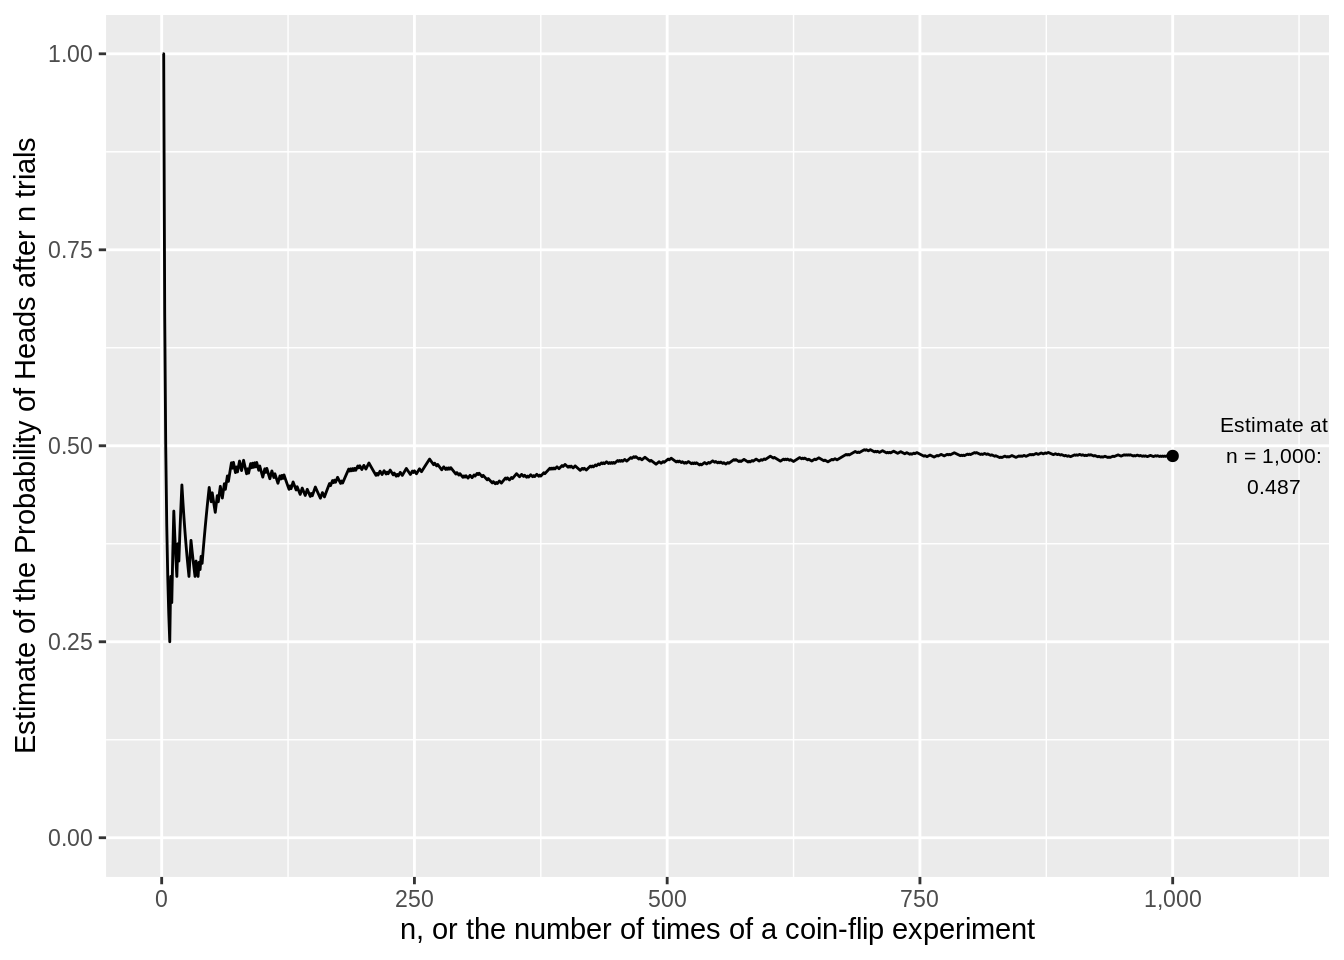
\includegraphics{prefresher_files/figure-latex/llnsim-1.pdf}
\caption{\label{fig:llnsim}As the number of coin tosses goes to infinity, the average probabiity of heads converges to 0.5}
\end{figure}

\hypertarget{sequences}{%
\section{Sequences}\label{sequences}}

We need a couple of steps until we get to limit theorems in probability. First we will introduce a ``sequence'', then we will think about the limit of a sequence, then we will think about the limit of a \emph{function}.

A \textbf{sequence} \[\{x_n\}=\{x_1, x_2, x_3, \ldots, x_n\}\] is an ordered set of real numbers, where \(x_1\) is the first term in the sequence and \(y_n\) is the \(n\)th term. Generally, a sequence is infinite, that is it extends to \(n=\infty\). We can also write the sequence as \[\{x_n\}^\infty_{n=1}\]

where the subscript and superscript are read together as ``from 1 to infinity.''

\BeginKnitrBlock{example}[Sequences]
\protect\hypertarget{exm:seqbehav}{}{\label{exm:seqbehav} \iffalse (Sequences) \fi{} }
How does these sequence behave?

\begin{enumerate}
\def\labelenumi{\arabic{enumi}.}
\tightlist
\item
  \(\{A_n\}=\left\{ 2-\frac{1}{n^2} \right\}\)
\item
  \(\{B_n\}=\left\{\frac{n^2+1}{n} \right\}\)
\item
  \(\{C_n\}=\left\{(-1)^n \left(1-\frac{1}{n}\right) \right\}\)
\end{enumerate}
\EndKnitrBlock{example}

We find the sequence by simply ``plugging in'' the integers into each \(n\). The important thing is to get a sense of how these numbers are going to change. Example 1's numbers seem to come closer and closer to 2, but will it ever surpass 2? Example 2's numbers are also increasing each time, but will it hit a limit? What is the pattern in Example 3? Graphing helps you make this point more clearly. See the sequence of \(n = 1, ...20\) for each of the three examples in Figure \ref{fig:seqabc}.

\begin{figure}
\centering
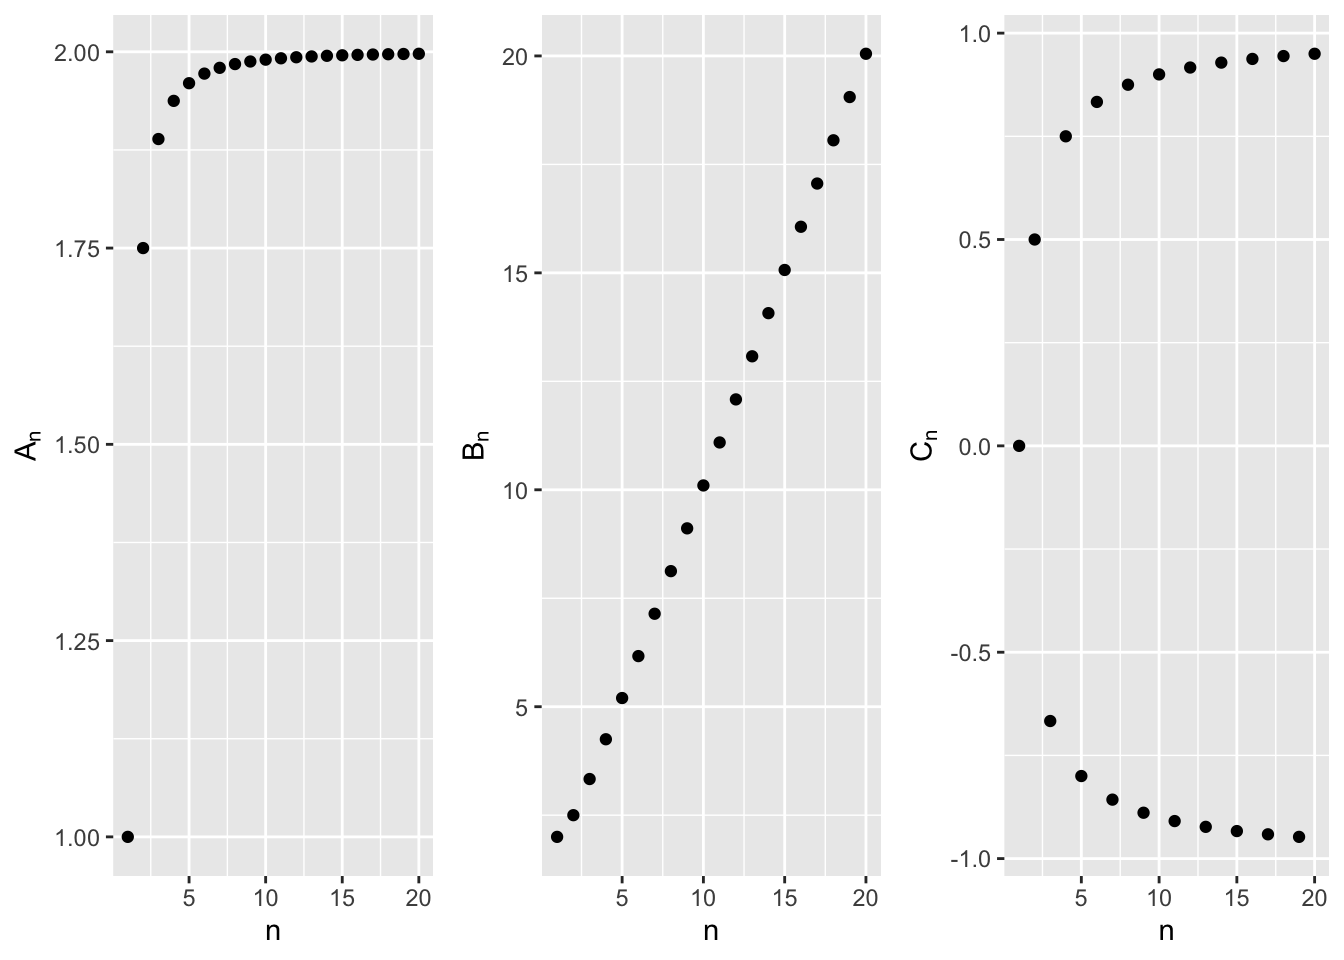
\includegraphics{prefresher_files/figure-latex/seqabc-1.pdf}
\caption{\label{fig:seqabc}Behavior of Some Sequences}
\end{figure}

\hypertarget{the-limit-of-a-sequence}{%
\section{The Limit of a Sequence}\label{the-limit-of-a-sequence}}

The notion of ``converging to a limit'' is the behavior of the points in Example \ref{exm:seqbehav}. In some sense, that's the counterfactual we want to know. What happens as \(n\rightarrow \infty\)?

\begin{enumerate}
\def\labelenumi{\arabic{enumi}.}
\tightlist
\item
  Sequences like 1 above that converge to a limit.
\item
  Sequences like 2 above that increase without bound.
\item
  Sequences like 3 above that neither converge nor increase without bound --- alternating over the number line.
\end{enumerate}

\BeginKnitrBlock{definition}
\protect\hypertarget{def:unnamed-chunk-2}{}{\label{def:unnamed-chunk-2} }The sequence \(\{y_n\}\) has the limit \(L\), which we write as \[\lim\limits_{n \to \infty} y_n =L\], if for any \(\epsilon>0\) there is an integer \(N\) (which depends on \(\epsilon\)) with the property that \(|y_n -L|<\epsilon\) for each \(n>N\). \(\{y_n\}\) is said to converge to \(L\). If the above does not hold, then \(\{y_n\}\) diverges.
\EndKnitrBlock{definition}

We can also express the behavior of a sequence as bounded or not:

\begin{enumerate}
\def\labelenumi{\arabic{enumi}.}
\tightlist
\item
  Bounded: if \(|y_n|\le K\) for all \(n\)
\item
  Monotonically Increasing: \(y_{n+1}>y_n\) for all \(n\)
\item
  Monotonically Decreasing: \(y_{n+1}<y_n\) for all \(n\)
\end{enumerate}

A limit is \emph{unique}: If \(\{y_n\}\) converges, then the limit \(L\) is unique.

If a sequence converges, then the sum of such sequences also converges. Let \(\lim\limits_{n \to \infty} y_n = y\) and \(\lim\limits_{n \to \infty} z_n =z\). Then

\begin{enumerate}
\def\labelenumi{\arabic{enumi}.}
\tightlist
\item
  \(\lim\limits_{n \to \infty} [k y_n + \ell z_n]= k y + \ell z\)
\item
  \(\lim\limits_{n \to \infty} y_n z_n = yz\)
\item
  \(\lim\limits_{n \to \infty} \frac{y_n}{z_n} = \frac{y}{z}\), provided \(z\neq 0\)
\end{enumerate}

This looks reasonable enough. The harder question, obviously is when the parts of the fraction \emph{don't} converge. If \(\lim_{n\to\infty} y_n = \infty\) and \(\lim_{n\to\infty} z_n = \infty\), What is \(\lim_{n\to\infty} y_n - z_n\)? What is \(\lim_{n\to\infty} \frac{y_n}{z_n}\)?

It is nice for a sequence to converge in limit. We want to know if complex-looking sequences converge or not. The name of the game here is to break that complex sequence up into sums of simple fractions where \(n\) only appears in the denominator: \(\frac{1}{n}, \frac{1}{n^2}\), and so on. Each of these will converge to 0, because the denominator gets larger and larger. Then, because of the properties above, we can then find the final sequence.

\BeginKnitrBlock{example}[Simplifying a Fraction into Sums]
\protect\hypertarget{exm:unnamed-chunk-3}{}{\label{exm:unnamed-chunk-3} \iffalse (Simplifying a Fraction into Sums) \fi{} }Find the limit of
\[\lim_{n\to \infty} \frac{n + 3}{n},\]
\EndKnitrBlock{example}

\BeginKnitrBlock{solution}
\iffalse{} {Solution. } \fi{}At first glance, \(n + 3\) and \(n\) both grow to \(\infty\), so it looks like we need to divide infinity by infinity. However, we can express this fraction as a sum, then the limits apply separately:

\[\lim_{n\to \infty} \frac{n + 3}{n} = \lim_{n\to \infty} \left(1 + \frac{3}{n}\right) =  \underbrace{\lim_{n\to \infty}1}_{1} +  \underbrace{\lim_{n\to \infty}\left(\frac{3}{n}\right)}_{0}\]

so, the limit is actually 1.
\EndKnitrBlock{solution}

After some practice, the key to intuition is whether one part of the fraction grows ``faster'' than another. If the denominator grows faster to infinity than the numerator, then the fraction will converge to 0, even if the numerator will also increase to infinity. In a sense, limits show how not all infinities are the same.

\BeginKnitrBlock{exercise}
\protect\hypertarget{exr:limseq2}{}{\label{exr:limseq2} }Find the following limits of sequences, then explain in English the intuition for why that is the case.

\begin{enumerate}
\def\labelenumi{\arabic{enumi}.}
\tightlist
\item
  \(\lim\limits_{n\to\infty} \frac{2n}{n^2 + 1}\)
\item
  \(\lim\limits_{n\to\infty} (n^3 - 100n^2)\)
\end{enumerate}
\EndKnitrBlock{exercise}

\hypertarget{limitsfun}{%
\section{Limits of a Function}\label{limitsfun}}

We've now covered functions and just covered limits of sequences, so now is the time to combine the two.

A function \(f\) is a compact representation of some behavior we care about. Like for sequences, we often want to know if \(f(x)\) approaches some number \(L\) as its independent variable \(x\) moves to some number \(c\) (which is usually 0 or \(\pm\infty\)). If it does, we say that the limit of \(f(x)\), as \(x\) approaches \(c\), is \(L\): \(\lim\limits_{x \to c} f(x)=L\). Unlike a sequence, \(x\) is a continuous number, and we can move in decreasing order as well as increasing.

For a limit \(L\) to exist, the function \(f(x)\) must approach \(L\) from both the left (increasing) and the right (decreasing).

\BeginKnitrBlock{definition}[Limit of a function]
\protect\hypertarget{def:unnamed-chunk-5}{}{\label{def:unnamed-chunk-5} \iffalse (Limit of a function) \fi{} }Let \(f(x)\) be defined at each point in some open interval containing the point \(c\). Then \(L\) equals \(\lim\limits_{x \to c} f(x)\) if for any (small positive) number \(\epsilon\), there exists a corresponding number \(\delta>0\) such that if \(0<|x-c|<\delta\), then \(|f(x)-L|<\epsilon\).
\EndKnitrBlock{definition}

A neat, if subtle result is that \(f(x)\) does not necessarily have to be defined at \(c\) for \(\lim\limits_{x \to c}\) to exist.

Properties: Let \(f\) and \(g\) be functions with \(\lim\limits_{x \to c} f(x)=k\) and \(\lim\limits_{x \to c} g(x)=\ell\).

\begin{enumerate}
\def\labelenumi{\arabic{enumi}.}
\tightlist
\item
  \(\lim\limits_{x \to c}[f(x)+g(x)]=\lim\limits_{x \to c} f(x)+ \lim\limits_{x \to c} g(x)\)
\item
  \(\lim\limits_{x \to c} kf(x) = k\lim\limits_{x \to c} f(x)\)
\item
  \(\lim\limits_{x \to c} f(x) g(x) = \left[\lim\limits_{x \to c} f(x)\right]\cdot \left[\lim\limits_{x \to c} g(x)\right]\)
\item
  \(\lim\limits_{x \to c} \frac{f(x)}{g(x)} = \frac{\lim\limits_{x \to c} f(x)}{\lim\limits_{x \to c} g(x)}\), provided \(\lim\limits_{x \to c} g(x)\ne 0\).
\end{enumerate}

Simple limits of functions can be solved as we did limits of sequences. Just be careful which part of the function is changing.

\BeginKnitrBlock{example}[Limits of Functions]
\protect\hypertarget{exm:limfun1}{}{\label{exm:limfun1} \iffalse (Limits of Functions) \fi{} }Find the limit of the following functions.

\begin{enumerate}
\def\labelenumi{\arabic{enumi}.}
\tightlist
\item
  \(\lim_{x \to c} k\)
\item
  \(\lim_{x \to c} x\)
\item
  \(\lim_{x\to 2} (2x-3)\)
\item
  \(\lim_{x \to c} x^n\)
\end{enumerate}
\EndKnitrBlock{example}

Limits can get more complex in roughly two ways. First, the functions may become large polynomials with many moving pieces. Second,the functions may become discontinuous.

The function can be thought of as a more general or ``smooth'' version of sequences. For example,

\BeginKnitrBlock{exercise}[Limits of a Fraction of Functions]
\protect\hypertarget{exr:limfunmax}{}{\label{exr:limfunmax} \iffalse (Limits of a Fraction of Functions) \fi{} }
Find the limit of

\[\lim_{x\to\infty} \frac{(x^4 +3x−99)(2−x^5)}{(18x^7 +9x^6 −3x^2 −1)(x+1)}\]
\EndKnitrBlock{exercise}

Now, the functions will become a bit more complex:

\BeginKnitrBlock{exercise}
\protect\hypertarget{exr:discontlim}{}{\label{exr:discontlim} }Solve the following limits of functions

\begin{enumerate}
\def\labelenumi{\arabic{enumi}.}
\tightlist
\item
  \(\lim\limits_{x\to 0} |x|\)
\item
  \(\lim\limits_{x\to 0} \left(1+\frac{1}{x^2}\right)\)
\end{enumerate}
\EndKnitrBlock{exercise}

So there are a few more alternatives about what a limit of a function could be:

\begin{enumerate}
\def\labelenumi{\arabic{enumi}.}
\tightlist
\item
  Right-hand limit: The value approached by \(f(x)\) when you move from right to left.
\item
  Left-hand limit: The value approached by \(f(x)\) when you move from left to right.
\item
  Infinity: The value approached by \(f(x)\) as x grows infinitely large. Sometimes this may be a number; sometimes it might be \(\infty\) or \(-\infty\).
\item
  Negative infinity: The value approached by \(f(x)\) as x grows infinitely negative. Sometimes this may be a number; sometimes it might be \(\infty\) or \(-\infty\).
\end{enumerate}

The distinction between left and right becomes important when the function is not determined for some values of \(x\). What are those cases in the examples below?

\begin{figure}
\centering
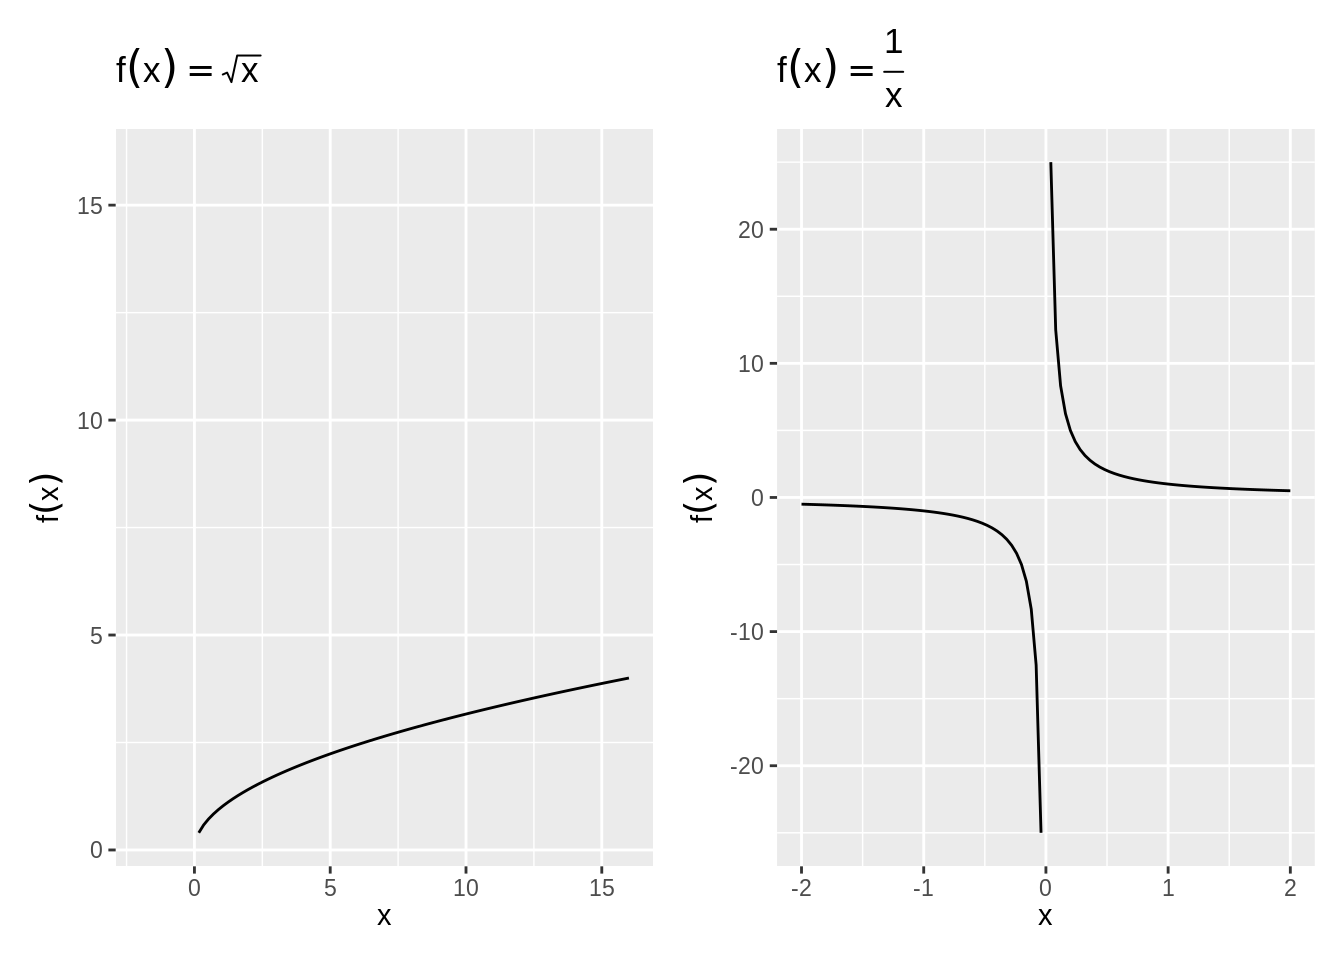
\includegraphics{prefresher_files/figure-latex/unnamed-chunk-6-1.pdf}
\caption{\label{fig:unnamed-chunk-6}Functions which are not defined in some areas}
\end{figure}

\hypertarget{continuity}{%
\section{Continuity}\label{continuity}}

To repeat a finding from the limits of functions: \(f(x)\) does not necessarily have to be defined at \(c\) for \(\lim\limits_{x \to c}\) to exist. Functions that have breaks in their lines are called discontinuous. Functions that have no breaks are called continuous. Continuity is a concept that is more fundamental to, but related to that of ``differentiability'', which we will cover next in calculus.

\BeginKnitrBlock{definition}[Continuity]
\protect\hypertarget{def:unnamed-chunk-7}{}{\label{def:unnamed-chunk-7} \iffalse (Continuity) \fi{} }Suppose that the domain of the function \(f\) includes an open interval containing the point \(c\). Then \(f\) is continuous at \(c\) if \(\lim\limits_{x \to c} f(x)\) exists and if \(\lim\limits_{x \to c} f(x)=f(c)\). Further, \(f\) is continuous on an open interval \((a,b)\) if it is continuous at each point in the interval.
\EndKnitrBlock{definition}

To prove that a function is continuous for all points is beyond this practical introduction to math, but the general intuition can be grasped by graphing.

\BeginKnitrBlock{example}[Continuous and Discontinuous Functions]
\protect\hypertarget{exm:contdiscont}{}{\label{exm:contdiscont} \iffalse (Continuous and Discontinuous Functions) \fi{} }
For each function, determine if it is continuous or discontinuous.

\begin{enumerate}
\def\labelenumi{\arabic{enumi}.}
\tightlist
\item
  \(f(x) = \sqrt{x}\)
\item
  \(f(x) = e^x\)
\item
  \(f(x) = 1 + \frac{1}{x^2}\)
\item
  \(f(x) = \text{floor}(x)\).
\end{enumerate}

The floor is the smaller of the two integers bounding a number. So \(\text{floor}(x = 2.999) = 2\), \(\text{floor}(x = 2.0001) = 2\), and \(\text{floor}(x = 2) = 2.\)
\EndKnitrBlock{example}

\BeginKnitrBlock{solution}
\iffalse{} {Solution. } \fi{}In Figure \ref{fig:fig-contdiscont}, we can see that the first two functions are continuous, and the next two are discontinuous. \(f(x) = 1 + \frac{1}{x^2}\) is discontinuous at \(x= 0\), and \(f(x) = \text{floor}(x)\) is discontinuous at each whole number.
\EndKnitrBlock{solution}

\begin{figure}
\centering
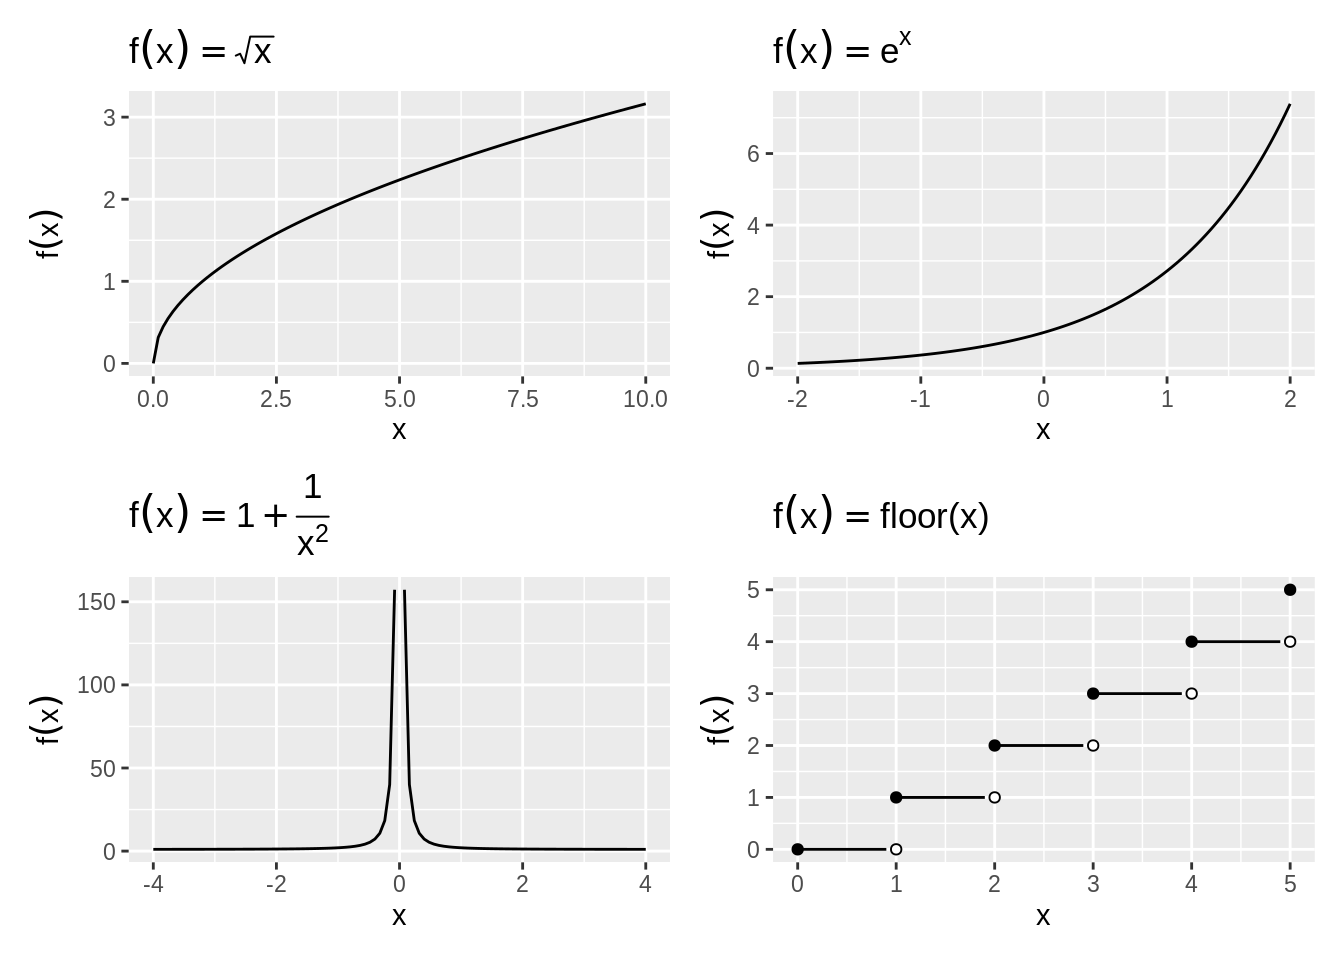
\includegraphics{prefresher_files/figure-latex/fig-contdiscont-1.pdf}
\caption{\label{fig:fig-contdiscont}Continuous and Discontinuous Functions}
\end{figure}

Some properties of continuous functions:

\begin{enumerate}
\def\labelenumi{\arabic{enumi}.}
\tightlist
\item
  If \(f\) and \(g\) are continuous at point \(c\), then \(f+g\), \(f-g\), \(f \cdot g\), \(|f|\), and \(\alpha f\) are continuous at point \(c\) also. \(f/g\) is continuous, provided \(g(c)\ne 0\).
\item
  Boundedness: If \(f\) is continuous on the closed bounded interval \([a,b]\), then there is a number \(K\) such that \(|f(x)|\le K\) for each \(x\) in \([a,b]\).
\item
  Max/Min: If \(f\) is continuous on the closed bounded interval \([a,b]\), then \(f\) has a maximum and a minimum on \([a,b]\). They may be located at the end points.
\end{enumerate}

\BeginKnitrBlock{exercise}[Limit when Denominator converges to 0]
\protect\hypertarget{exr:discontdraw}{}{\label{exr:discontdraw} \iffalse (Limit when Denominator converges to 0) \fi{} }
Let \[f(x) = \frac{x^2 + 2x}{x}.\]

\begin{enumerate}
\def\labelenumi{\arabic{enumi}.}
\tightlist
\item
  Graph the function. Is it defined everywhere?
\item
  What is the functions limit at \(x \rightarrow 0\)?
\end{enumerate}
\EndKnitrBlock{exercise}

\hypertarget{answers-to-examples}{%
\section*{Answers to Examples}\label{answers-to-examples}}
\addcontentsline{toc}{section}{Answers to Examples}

Example \ref{exm:seqbehav}

\BeginKnitrBlock{solution}
\iffalse{} {Solution. } \fi{}

\begin{enumerate}
\def\labelenumi{\arabic{enumi}.}
\tightlist
\item
  \(\{A_n\}=\left\{ 2-\frac{1}{n^2} \right\} = \left\{1, \frac{7}{4}, \frac{17}{9}, \frac{31}{16}, \frac{49}{25}, \ldots\right\} = 2\)
\item
  \(\{B_n\}=\left\{\frac{n^2+1}{n} \right\} = \left\{2, \frac{5}{2}, \frac{10}{3}, \frac{17}{4}..., \right\}\)
\item
  \(\{C_n\}=\left\{(-1)^n \left(1-\frac{1}{n}\right) \right\} = \left\{0, \frac{1}{2}, -\frac{2}{3}, \frac{3}{4}, -\frac{4}{5}\right\}\)
\end{enumerate}
\EndKnitrBlock{solution}

Exercise \ref{exr:limseq2}

Example \ref{exm:limfun1}

\BeginKnitrBlock{solution}
\iffalse{} {Solution. } \fi{}

\begin{enumerate}
\def\labelenumi{\arabic{enumi}.}
\tightlist
\item
  \(k\)
\item
  \(c\)
\item
  \(\lim_{x\to 2} (2x-3) = 2\lim\limits_{x\to 2} x - 3\lim\limits_{x\to 2} 1 = 1\)
\item
  \(\lim_{x \to c} x^n = \lim\limits_{x \to c} x \cdots[\lim\limits_{x \to c} x] = c\cdots c =c^n\)
\end{enumerate}
\EndKnitrBlock{solution}

Exercise \ref{exr:limfunmax}

\BeginKnitrBlock{solution}
\iffalse{} {Solution. } \fi{}Although this function seems large, the thing our eyes should focus on is where the highest order polynomial remains. That will grow the fastest, so if the highest order term is on the denominator, the fraction will converge to 0, if it is on the numerator it will converge to negative infinity. Previewing the multiplication by hand, we can see that the \(-x^9\) on the numerator will be the largest power. So the answer will be \(-\infty\). We can also confirm this by writing out fractions:

\begin{align*}  
& \lim_{x\to\infty}\frac{\left(1 + \frac{3}{x^3} - \frac{99}{4x^4}\right)\left(-\frac{2}{x^5} + 1\right)}{\left(1 + \frac{9}{18x} - \frac{3}{18x^5} - \frac{1}{18x^7} \right)\left(1 + \frac{1}{x}\right)} \\
&\times \frac{x^4}{1} \times -\frac{x^5}{1} \times \frac{1}{18x^7}\times \frac{1}{x}\\
=& 1 \times \lim_{-x\to\infty} \frac{x}{18}
\end{align*}
\EndKnitrBlock{solution}

Exercise \ref{exr:discontdraw}

\BeginKnitrBlock{solution}
\iffalse{} {Solution. } \fi{}
See Figure \ref{fig:fig-hole-0}.

Divide each part by \(x\), and we get \(x + \frac{2}{x}\) on the numerator, \(1\) on the denominator. So, without worrying about a function being not defined, we can say \(\lim_{x\to 0}f(x) = 0\).
\EndKnitrBlock{solution}

\begin{figure}
\centering
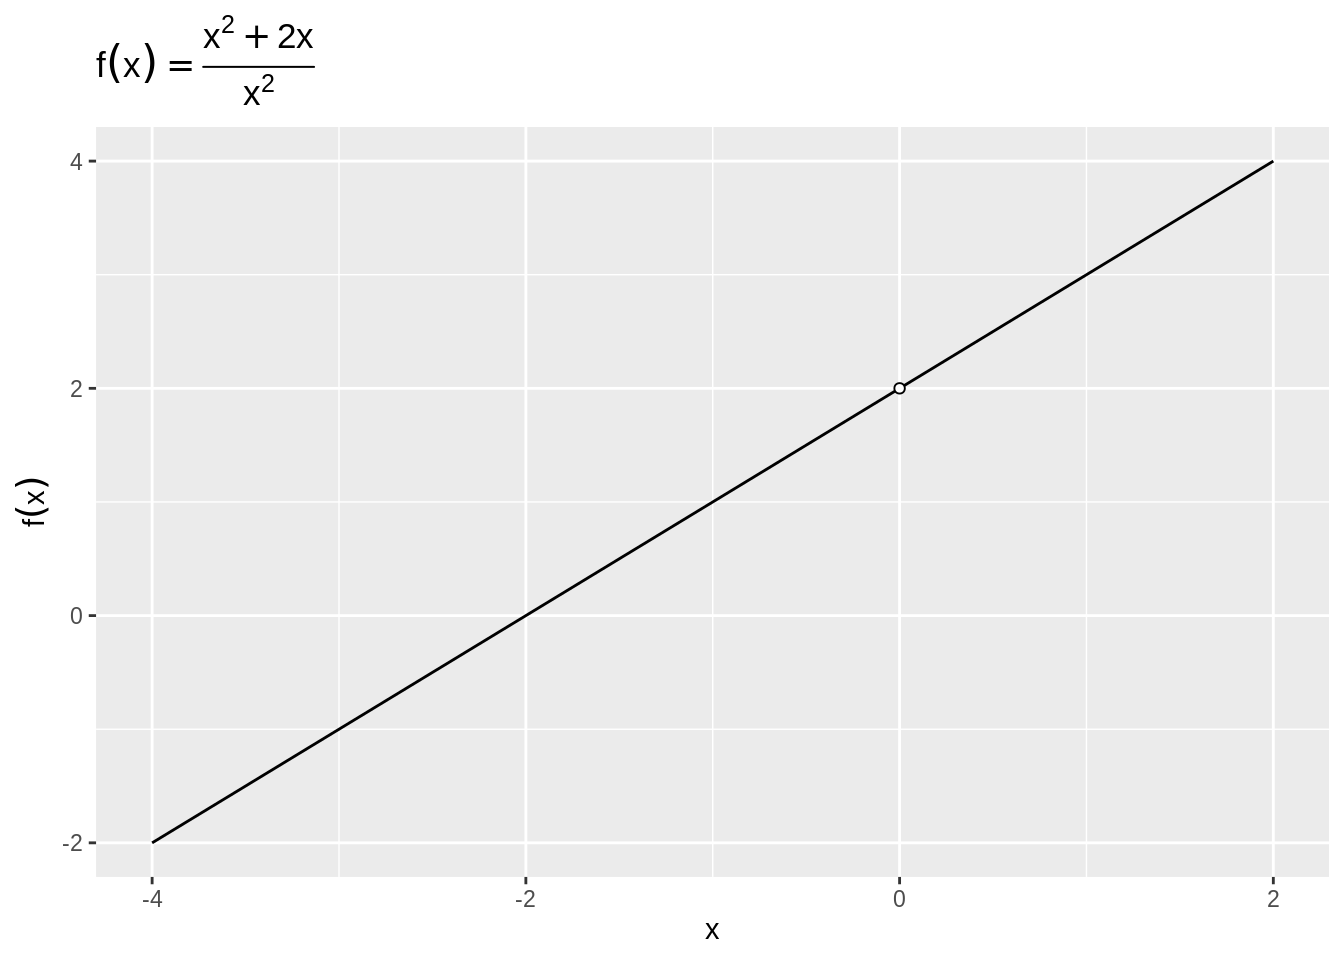
\includegraphics{prefresher_files/figure-latex/fig-hole-0-1.pdf}
\caption{\label{fig:fig-hole-0}A function undedefined at x = 0}
\end{figure}

\hypertarget{derivatives}{%
\chapter{Calculus}\label{derivatives}}

Calculus is a fundamental part of any type of statistics exercise. Although you may not be taking derivatives and integral in your daily work as an analyst, calculus undergirds many concepts we use: maximization, expectation, and cumulative probability.

\hypertarget{example-the-mean-is-a-type-of-integral}{%
\section*{Example: The Mean is a Type of Integral}\label{example-the-mean-is-a-type-of-integral}}
\addcontentsline{toc}{section}{Example: The Mean is a Type of Integral}

The average of a quantity is a type of weighted mean, where the potential values are weighted by their likelihood, loosely speaking. The integral is actually a general way to describe this weighted average when there are conceptually an infinite number of potential values.

If \(X\) is a continuous random variable, its expected value \(E(X)\) -- the center of mass -- is given by

\[E(X) = \int^{\infty}_{-\infty}x f(x) dx\]

where \(f(x)\) is the probability density function of \(X\).

This is a continuous version of the case where \(X\) is discrete, in which case

\[E(X) = \sum^\infty_{j=1} x_j P(X = x_j)\]

even more concretely, if the potential values of \(X\) are finite, then we can write out the expected value as a weighted mean, where the weights is the probability that the value occurs.

\[E(X) = \large \sum_{x} \quad\left( \underbrace{x}_{\text{value}}\cdot \underbrace{P(X = x)}_{\text{weight, or PMF}}\right)\]

\hypertarget{derivintro}{%
\section{Derivatives}\label{derivintro}}

The derivative of \(f\) at \(x\) is its rate of change at \(x\): how much \(f(x)\) changes with a change in \(x\). The rate of change is a fraction --- rise over run --- but because not all lines are straight and the rise over run formula will give us different values depending on the range we examine, we need to take a limit (Section \ref{limits-precalc}).

\BeginKnitrBlock{definition}[Derivative]
\protect\hypertarget{def:unnamed-chunk-15}{}{\label{def:unnamed-chunk-15} \iffalse (Derivative) \fi{} }Let \(f\) be a function whose domain includes an open interval containing the point \(x\). The derivative of \(f\) at \(x\) is given by

\[\frac{d}{dx}f(x) =\lim\limits_{h\to 0} \frac{f(x+h)-f(x)}{(x+h)-x} = \lim\limits_{h\to 0} \frac{f(x+h)-f(x)}{h}
\]

There are a two main ways to denote a derivate:

\begin{itemize}
\tightlist
\item
  Leibniz Notation: \(\frac{d}{dx}(f(x))\)
\item
  Prime or Lagrange Notation: \(f'(x)\)
\end{itemize}
\EndKnitrBlock{definition}

If \(f(x)\) is a straight line, the derivative is the slope. For a curve, the slope changes by the values of \(x\), so the derivative is the slope of the line tangent to the curve at \(x\). See, For example, Figure \ref{fig:derivsimple}.

\begin{figure}
\centering
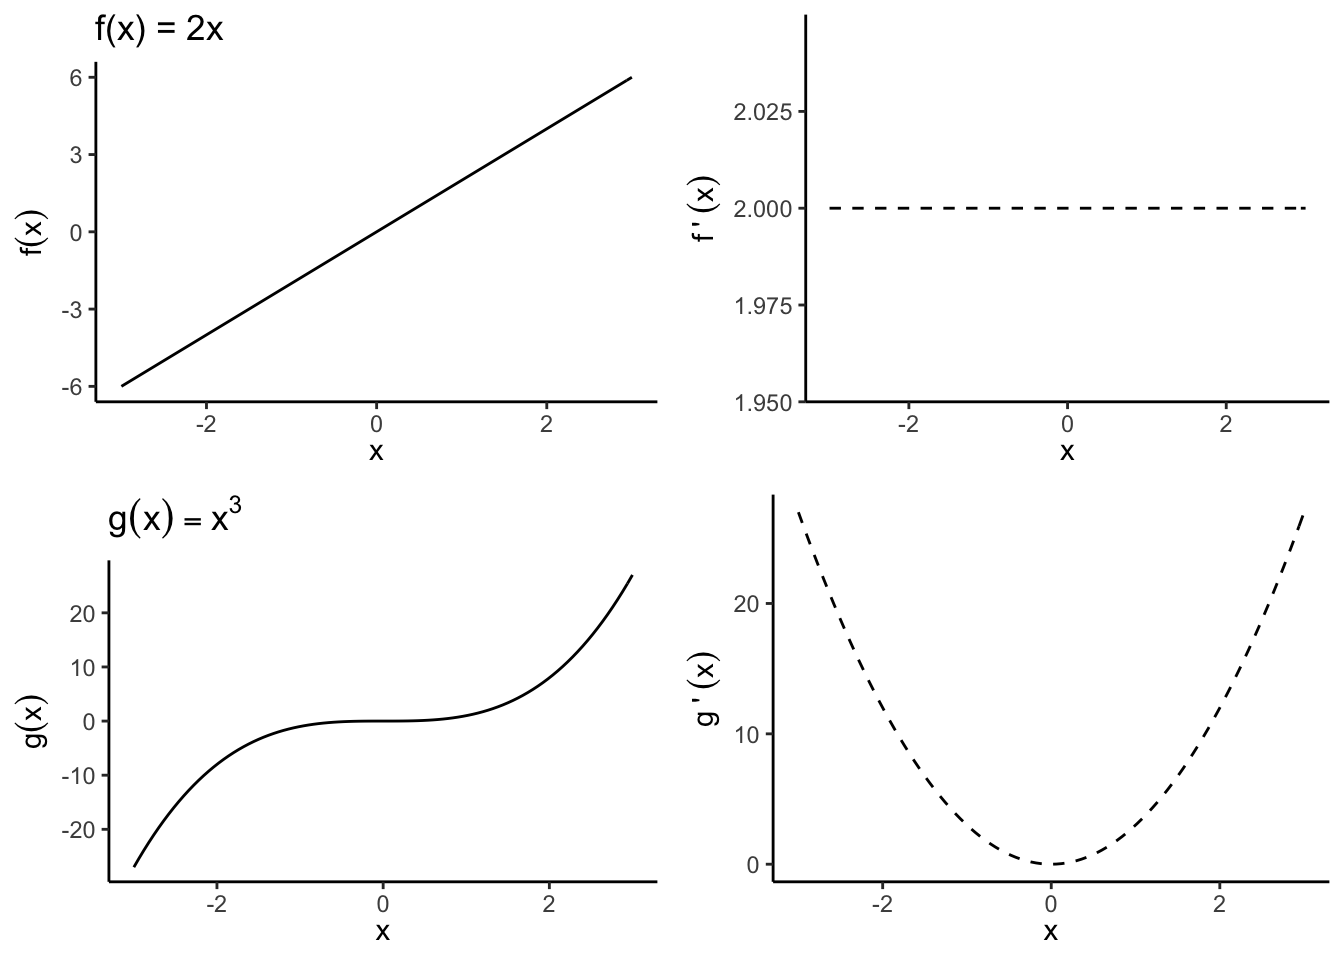
\includegraphics{prefresher_files/figure-latex/derivsimple-1.pdf}
\caption{\label{fig:derivsimple}The Derivative as a Slope}
\end{figure}

If \(f'(x)\) exists at a point \(x_0\), then \(f\) is said to be \textbf{differentiable} at \(x_0\). That also implies that \(f(x)\) is continuous at \(x_0\).

\hypertarget{properties-of-derivatives}{%
\subsection*{Properties of derivatives}\label{properties-of-derivatives}}
\addcontentsline{toc}{subsection}{Properties of derivatives}

Suppose that \(f\) and \(g\) are differentiable at \(x\) and that \(\alpha\) is a constant. Then the functions \(f\pm g\), \(\alpha f\), \(f g\), and \(f/g\) (provided \(g(x)\ne 0\)) are also differentiable at \(x\). Additionally,

\textbf{Constant rule:} \[\left[k f(x)\right]' = k f'(x)\]

\textbf{Sum rule:} \[\left[f(x)\pm g(x)\right]' = f'(x)\pm g'(x)\]

With a bit more algebra, we can apply the definition of derivatives to get a formula for of the derivative of a product and a derivative of a quotient.

\textbf{Product rule:} \[\left[f(x)g(x)\right]^\prime = f^\prime(x)g(x)+f(x)g^\prime(x)\]

\textbf{Quotient rule:} \[\left[f(x)/g(x)\right]^\prime = \frac{f^\prime(x)g(x) - f(x)g^\prime(x)}{[g(x)]^2}, ~g(x)\neq 0\]

Finally, one way to think of the power of derivatives is that it takes a function a notch down in complexity. The power rule applies to any higher-order function:

\textbf{Power rule:} \[\left[x^k\right]^\prime = k x^{k-1}\]

For any real number \(k\) (that is, both whole numbers and fractions). The power rule is proved \textbf{by induction}, a neat method of proof used in many fundamental applications to prove that a general statement holds for every possible case, even if there are countably infinite cases. We'll show a simple case where \(k\) is an integer here.

\BeginKnitrBlock{proof}[Proof of Power Rule by Induction]
\iffalse{} {Proof (Proof of Power Rule by Induction). } \fi{}
We would like to prove that

\[\left[x^k\right]^\prime = k x^{k-1}\]
for any integer \(k\).

First, consider the first case (the base case) of \(k = 1\). We can show by the definition of derivatives (setting \(f(x) = x^1 = 1\)) that

\[[x^1]^\prime = \lim_{h \rightarrow 0}\frac{(x + h) - x}{(x + h) - x}= 1.\]

Because \(1\) is also expressed as \(1 x^{1- 1}\), the statement we want to prove holds for the case \(k =1\).

Now, \emph{assume} that the statement holds for some integer \(m\). That is, assume
\[\left[x^m\right]^\prime = m x^{m-1}\]

Then, for the case \(m + 1\), using the product rule above, we can simplify

\begin{align*}
\left[x^{m + 1}\right]^\prime &= [x^{m}\cdot x]^\prime\\
&= (x^m)^\prime\cdot x + (x^m)\cdot (x)^\prime\\
&= m x^{m - 1}\cdot x + x^m ~~\because \text{by previous assumption}\\
&= mx^m + x^m\\
&= (m + 1)x^m\\
&= (m + 1)x^{(m + 1) - 1}
\end{align*}

Therefore, the rule holds for the case \(k = m + 1\) once we have assumed it holds for \(k = m\). Combined with the first case, this completes proof by induction -- we have now proved that the statement holds for all integers \(k = 1, 2, 3, \cdots\).

To show that it holds for real fractions as well, we can prove expressing that exponent by a fraction of two integers.
\EndKnitrBlock{proof}

These ``rules'' become apparent by applying the definition of the derivative above to each of the things to be ``derived'', but these come up so frequently that it is best to repeat until it is muscle memory.

\BeginKnitrBlock{exercise}[Derivative of Polynomials]
\protect\hypertarget{exr:introderivatives}{}{\label{exr:introderivatives} \iffalse (Derivative of Polynomials) \fi{} }
For each of the following functions, find the first-order derivative \(f^\prime(x)\).

\begin{enumerate}
\def\labelenumi{\arabic{enumi}.}
\tightlist
\item
  \(f(x)=c\)
\item
  \(f(x)=x\)
\item
  \(f(x)=x^2\)
\item
  \(f(x)=x^3\)
\item
  \(f(x)=\frac{1}{x^2}\)
\item
  \(f(x)=(x^3)(2x^4)\)
\item
  \(f(x) = x^4 - x^3 + x^2 - x + 1\)
\item
  \(f(x) = (x^2 + 1)(x^3 - 1)\)
\item
  \(f(x) = 3x^2 + 2x^{1/3}\)
\item
  \(f(x)=\frac{x^2+1}{x^2-1}\)
\end{enumerate}
\EndKnitrBlock{exercise}

\hypertarget{derivpoly}{%
\section{Higher-Order Derivatives (Derivatives of Derivatives of Derivatives)}\label{derivpoly}}

The first derivative is applying the definition of derivatives on the function, and it can be expressed as

\[f'(x),  ~~ y',  ~~ \frac{d}{dx}f(x), ~~ \frac{dy}{dx}\]

We can keep applying the differentiation process to functions that are themselves derivatives. The derivative of \(f'(x)\) with respect to \(x\), would then be \[f''(x)=\lim\limits_{h\to 0}\frac{f'(x+h)-f'(x)}{h}\] and we can therefore call it the \textbf{Second derivative:}

\[f''(x), ~~ y'', ~~ \frac{d^2}{dx^2}f(x), ~~ \frac{d^2y}{dx^2}\]

Similarly, the derivative of \(f''(x)\) would be called the third derivative and is denoted \(f'''(x)\). And by extension, the \textbf{nth derivative} is expressed as \(\frac{d^n}{dx^n}f(x)\), \(\frac{d^ny}{dx^n}\).

\BeginKnitrBlock{example}[Succession of Derivatives]
\protect\hypertarget{exm:unnamed-chunk-16}{}{\label{exm:unnamed-chunk-16} \iffalse (Succession of Derivatives) \fi{} }\begin{align*}
f(x) &=x^3\\
f^{\prime}(x) &=3x^2\\
f^{\prime\prime}(x) &=6x \\
f^{\prime\prime\prime}(x) &=6\\
f^{\prime\prime\prime\prime}(x) &=0\\
\end{align*}
\EndKnitrBlock{example}

Earlier, in Section \ref{derivintro}, we said that if a function differentiable at a given point, then it must be continuous. Further, if \(f'(x)\) is itself continuous, then \(f(x)\) is called continuously differentiable. All of this matters because many of our findings about optimization (Section \ref{optim}) rely on differentiation, and so we want our function to be differentiable in as many layers. A function that is continuously differentiable infinitly is called ``smooth''. Some examples: \(f(x) = x^2\), \(f(x) = e^x\).

\hypertarget{composite-functions-and-the-chain-rule}{%
\section{Composite Functions and the Chain Rule}\label{composite-functions-and-the-chain-rule}}

As useful as the above rules are, many functions you'll see won't fit neatly in each case immediately. Instead, they will be functions of functions. For example, the difference between \(x^2 + 1^2\) and \((x^2 + 1)^2\) may look trivial, but the sum rule can be easily applied to the former, while it's actually not obvious what do with the latter.

\textbf{Composite functions} are formed by substituting one function into another and are denoted by \[(f\circ g)(x)=f[g(x)].\] To form \(f[g(x)]\), the range of \(g\) must be contained (at least in part) within the domain of \(f\). The domain of \(f\circ g\) consists of all the points in the domain of \(g\) for which \(g(x)\) is in the domain of \(f\).

\BeginKnitrBlock{example}
\protect\hypertarget{exm:unnamed-chunk-17}{}{\label{exm:unnamed-chunk-17} }Let \(f(x)=\log x\) for \(0<x<\infty\) and \(g(x)=x^2\) for \(-\infty<x<\infty\).

Then
\[(f\circ g)(x)=\log x^2, -\infty<x<\infty - \{0\}\]

Also
\[(g\circ f)(x)=[\log x]^2, 0<x<\infty\]

Notice that \(f\circ g\) and \(g\circ f\) are not the same functions.
\EndKnitrBlock{example}

With the notation of composite functions in place, now we can introduce a helpful additional rule that will deal with a derivative of composite functions as a chain of concentric derivatives.

\textbf{Chain Rule}:

Let \(y=(f\circ g)(x)= f[g(x)]\). The derivative of \(y\) with respect to \(x\) is \[\frac{d}{dx} \{ f[g(x)] \} = f'[g(x)] g'(x)\]

We can read this as: ``the derivative of the composite function \(y\) is the derivative of \(f\) evaluated at \(g(x)\), times the derivative of \(g\).''

The chain rule can be thought of as the derivative of the ``outside'' times the derivative of the ``inside'', remembering that the derivative of the outside function is evaluated at the value of the inside function.

\begin{itemize}
\tightlist
\item
  The chain rule can also be written as \[\frac{dy}{dx}=\frac{dy}{dg(x)} \frac{dg(x)}{dx}\] This expression does not imply that the \(dg(x)\)'s cancel out, as in fractions. They are part of the derivative notation and you can't separate them out or cancel them.)
\end{itemize}

\BeginKnitrBlock{example}[Composite Exponent]
\protect\hypertarget{exm:tothesix}{}{\label{exm:tothesix} \iffalse (Composite Exponent) \fi{} }Find \(f^\prime(x)\) for \(f(x) = (3x^2+5x-7)^6\).
\EndKnitrBlock{example}

The direct use of a chain rule is when the exponent of is itself a function, so the power rule could not have applied generaly:

\textbf{Generalized Power Rule}:

If \(f(x)=[g(x)]^p\) for any rational number \(p\), \[f^\prime(x) =p[g(x)]^{p-1}g^\prime(x)\]

\hypertarget{derivatives-of-natural-logs-and-the-exponent}{%
\section{Derivatives of natural logs and the exponent}\label{derivatives-of-natural-logs-and-the-exponent}}

Natural logs and exponents (they are inverses of each other; see Section \ref{logexponents}) crop up everywhere in statistics. Their derivative is a special case from the above, but quite elegant.

\BeginKnitrBlock{theorem}
\protect\hypertarget{thm:derivexplog}{}{\label{thm:derivexplog} }
The functions \(e^x\) and the natural logarithm \(\log(x)\) are continuous and differentiable in their domains, and their first derivate is
\[(e^x)^\prime = e^x\]
\[\log(x)^\prime = \frac{1}{x}\]

Also, when these are composite functions, it follows by the generalized power rule that

\[\left(e^{g(x)}\right)^\prime = e^{g(x)} \cdot g^\prime(x)\]
\[\left(\log g(x)\right)^\prime = \frac{g^\prime(x)}{g(x)}, ~~\text{if}~~ g(x) > 0\]
\EndKnitrBlock{theorem}

We will relegate the proofs to small excerpts.

\hypertarget{derivatives-of-natural-exponential-function-e}{%
\subsection*{\texorpdfstring{Derivatives of natural exponential function (\(e\))}{Derivatives of natural exponential function (e)}}\label{derivatives-of-natural-exponential-function-e}}
\addcontentsline{toc}{subsection}{Derivatives of natural exponential function (\(e\))}

To repeat the main rule in Theorem \ref{thm:derivexplog}, the intuition is that

\begin{enumerate}
\def\labelenumi{\arabic{enumi}.}
\tightlist
\item
  Derivative of \(e^x\) is itself: \(\frac{d}{dx}e^x = e^x\) (See Figure \ref{fig:fig-derivexponent})
\item
  Same thing if there were a constant in front: \(\frac{d}{dx}\alpha e^x = \alpha e^x\)
\item
  Same thing no matter how many derivatives there are in front: \(\frac{d^n}{dx^n} \alpha e^x = \alpha e^x\)
\item
  Chain Rule: When the exponent is a function of \(x\), remember to take derivative of that function and add to product. \(\frac{d}{dx}e^{g(x)}= e^{g(x)} g^\prime(x)\)
\end{enumerate}

\begin{figure}
\centering
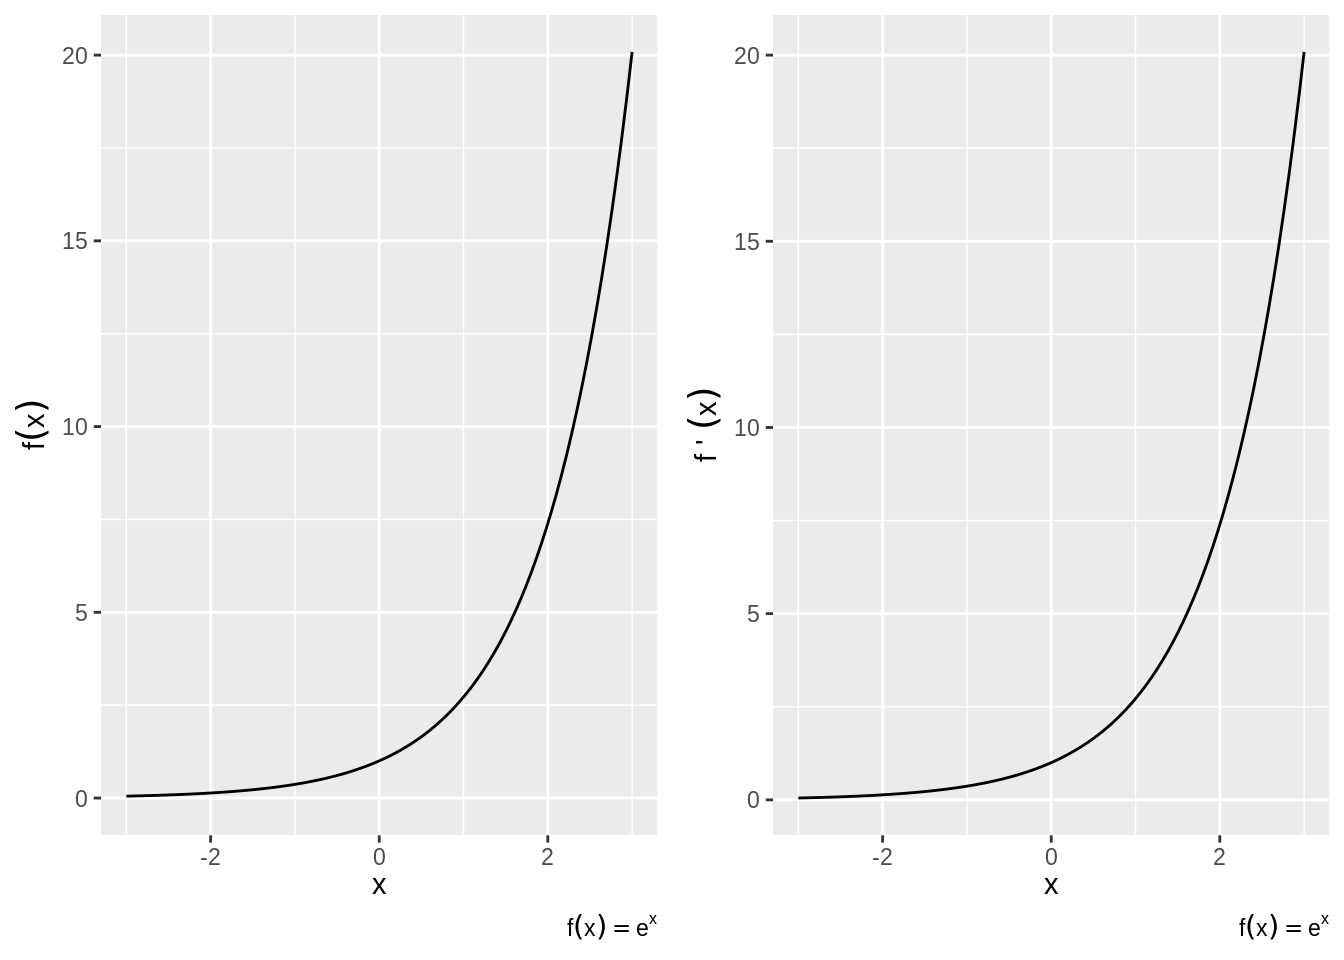
\includegraphics{prefresher_files/figure-latex/fig-derivexponent-1.pdf}
\caption{\label{fig:fig-derivexponent}Derivative of the Exponential Function}
\end{figure}

\BeginKnitrBlock{example}[Derivative of exponents]
\protect\hypertarget{exm:exmderivexp}{}{\label{exm:exmderivexp} \iffalse (Derivative of exponents) \fi{} }Find the derivative for the following.

\begin{enumerate}
\def\labelenumi{\arabic{enumi}.}
\tightlist
\item
  \(f(x)=e^{-3x}\)
\item
  \(f(x)=e^{x^2}\)
\item
  \(f(x)=(x-1)e^x\)
\end{enumerate}
\EndKnitrBlock{example}

\hypertarget{derivatives-of-log}{%
\subsection*{\texorpdfstring{Derivatives of \(\log\)}{Derivatives of \textbackslash{}log}}\label{derivatives-of-log}}
\addcontentsline{toc}{subsection}{Derivatives of \(\log\)}

The natural log is the mirror image of the natural exponent and has mirroring properties, again, to repeat the theorem,

\begin{enumerate}
\def\labelenumi{\arabic{enumi}.}
\tightlist
\item
  log prime x is one over x: \(\frac{d}{dx} \log x = \frac{1}{x}\) (Figure \ref{fig:fig-derivlog})
\item
  Exponents become multiplicative constants: \(\frac{d}{dx} \log x^k = \frac{d}{dx} k \log x = \frac{k}{x}\)
\item
  Chain rule again: \(\frac{d}{dx} \log u(x) = \frac{u'(x)}{u(x)}\quad\)
\item
  For any positive base \(b\), \(\frac{d}{dx} b^x = (\log b)\left(b^x\right)\).
\end{enumerate}

\begin{figure}
\centering
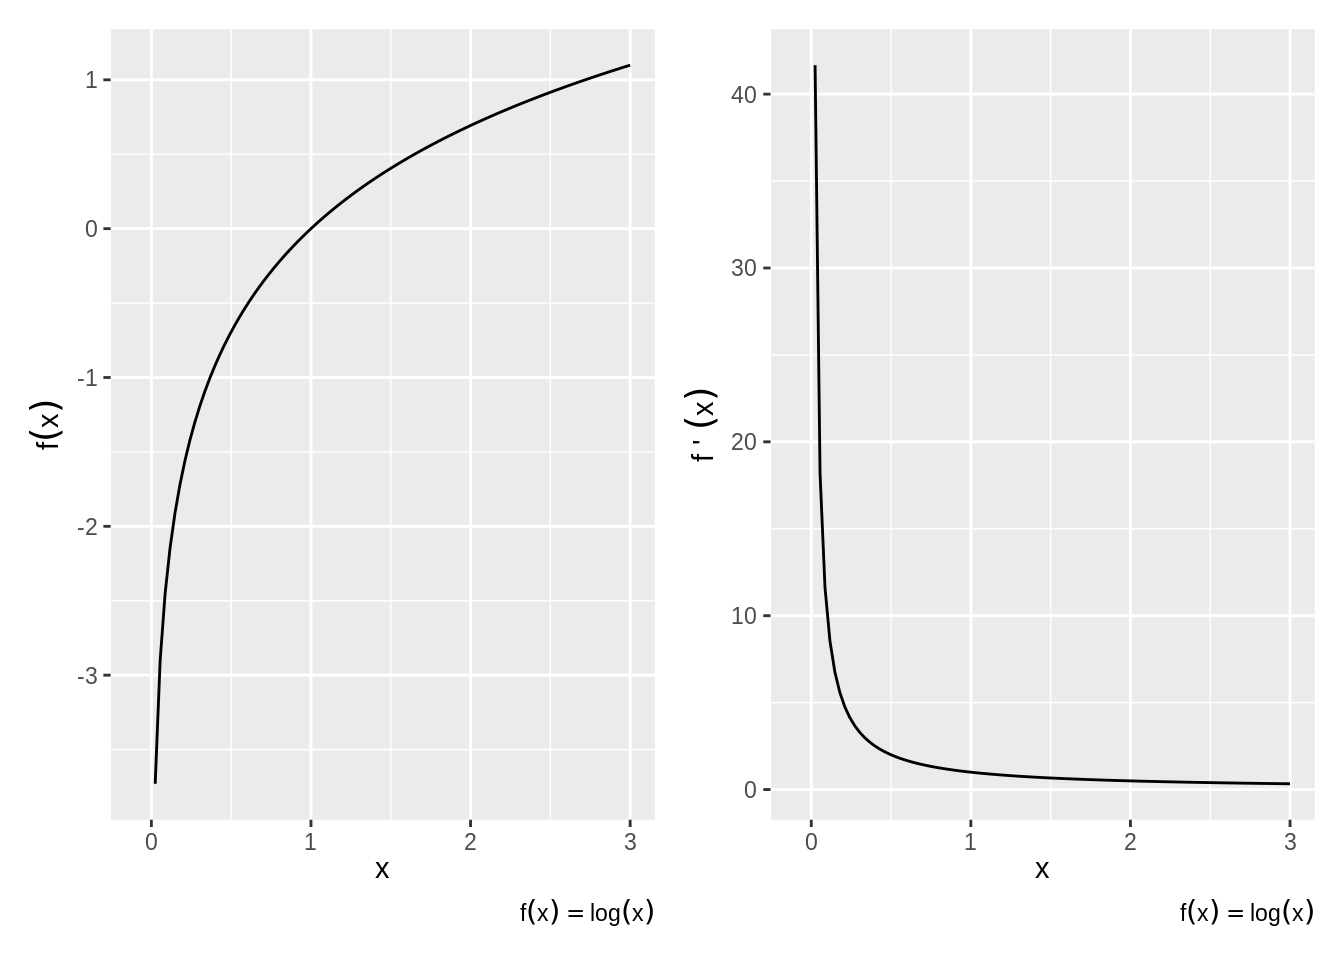
\includegraphics{prefresher_files/figure-latex/fig-derivlog-1.pdf}
\caption{\label{fig:fig-derivlog}Derivative of the Natural Log}
\end{figure}

\BeginKnitrBlock{example}[Derivative of logs]
\protect\hypertarget{exm:exmderivlog}{}{\label{exm:exmderivlog} \iffalse (Derivative of logs) \fi{} }Find \(dy/dx\) for the following.

\begin{enumerate}
\def\labelenumi{\arabic{enumi}.}
\tightlist
\item
  \(f(x)=\log(x^2+9)\)
\item
  \(f(x)=\log(\log x)\)
\item
  \(f(x)=(\log x)^2\)
\item
  \(f(x)=\log e^x\)
\end{enumerate}
\EndKnitrBlock{example}

\hypertarget{outline-of-proof}{%
\subsection*{Outline of Proof}\label{outline-of-proof}}
\addcontentsline{toc}{subsection}{Outline of Proof}

We actually show the derivative of the log first, and then the derivative of the exponential naturally follows.

The general derivative of the log at any base \(a\) is solvable by the definition of derivatives.

\begin{align*}
(\log_a x)^\prime = \lim\limits_{h\to 0} \frac{1}{h}\log_{a}\left(1 + \frac{h}{x}\right)
\end{align*}

Re-express \(g = \frac{h}{x}\) and get
\begin{align*}
(\log_a x)^\prime &= \frac{1}{x}\lim_{g\to 0}\log_{a} (1 + g)^{\frac{1}{g}}\\
&= \frac{1}{x}\log_a e
\end{align*}

By definition of \(e\). As a special case, when \(a = e\), then \((\log x)^\prime = \frac{1}{x}\).

Now let's think about the inverse, taking the derivative of \(y = a^x\).

\begin{align*}
y &= a^x \\
\Rightarrow \log y &= x \log a\\
\Rightarrow \frac{y^\prime}{y} &= \log a\\
\Rightarrow  y^\prime = y \log a\\
\end{align*}

Then in the special case where \(a = e\),

\[(e^x)^\prime = (e^x)\]

\hypertarget{partial-derivatives}{%
\section{Partial Derivatives}\label{partial-derivatives}}

What happens when there's more than variable that is changing?

\begin{quote}
If you can do ordinary derivatives, you can do partial derivatives: just hold all the other input variables constant except for the one you're differentiating with respect to. (Joe Blitzstein's Math Notes)
\end{quote}

Suppose we have a function \(f\) now of two (or more) variables and we want to determine the rate of change relative to one of the variables. To do so, we would find its partial derivative, which is defined similar to the derivative of a function of one variable.

\textbf{Partial Derivative}: Let \(f\) be a function of the variables \((x_1,\ldots,x_n)\). The partial derivative of \(f\) with respect to \(x_i\) is

\[\frac{\partial f}{\partial x_i} (x_1,\ldots,x_n) = \lim\limits_{h\to 0} \frac{f(x_1,\ldots,x_i+h,\ldots,x_n)-f(x_1,\ldots,x_i,\ldots,x_n)}{h}\]

Only the \(i\)th variable changes --- the others are treated as constants.

We can take higher-order partial derivatives, like we did with functions of a single variable, except now the higher-order partials can be with respect to multiple variables.

\BeginKnitrBlock{example}[More than one type of partial]
\protect\hypertarget{exm:unnamed-chunk-18}{}{\label{exm:unnamed-chunk-18} \iffalse (More than one type of partial) \fi{} }Notice that you can take partials with regard to different variables.

Suppose \(f(x,y)=x^2+y^2\). Then

\begin{align*}
\frac{\partial f}{\partial x}(x,y) &=\\
\frac{\partial f}{\partial y}(x,y) &=\\
\frac{\partial^2 f}{\partial x^2}(x,y) &=\\
\frac{\partial^2 f}{\partial x \partial y}(x,y) &=
\end{align*}
\EndKnitrBlock{example}

\BeginKnitrBlock{exercise}
\protect\hypertarget{exr:unnamed-chunk-19}{}{\label{exr:unnamed-chunk-19} }Let \(f(x,y)=x^3 y^4 +e^x -\log y\). What are the following partial derivaitves?

\begin{align*}
\frac{\partial f}{\partial x}(x,y) &=\\
\frac{\partial f}{\partial y}(x,y) &=\\
\frac{\partial^2 f}{\partial x^2}(x,y) &=\\
\frac{\partial^2 f}{\partial x \partial y}(x,y) &= 
\end{align*}
\EndKnitrBlock{exercise}

\hypertarget{taylorapprox}{%
\section{Taylor Series Approximation}\label{taylorapprox}}

A common form of approximation used in statistics involves derivatives. A Taylor series is a way to represent common functions as infinite series (a sum of infinite elements) of the function's derivatives at some point \(a\).

For example, Taylor series are very helpful in representing nonlinear (read: difficult) functions as linear (read: manageable) functions. One can thus \textbf{approximate} functions by using lower-order, finite series known as \textbf{Taylor polynomials}. If \(a=0\), the series is called a Maclaurin series.

Specifically, a Taylor series of a real or complex function \(f(x)\) that is infinitely differentiable in the neighborhood of point \(a\) is:

\begin{align*}
    f(x) &= f(a) + \frac{f'(a)}{1!} (x-a) +  \frac{f''(a)}{2!} (x-a)^2 + \cdots\\
     &= \sum_{n=0}^\infty \frac{f^{(n)} (a)}{n!} (x-a)^n
\end{align*}

\textbf{Taylor Approximation}: We can often approximate the curvature of a function \(f(x)\) at point \(a\) using a 2nd order Taylor polynomial around point \(a\):

\[f(x) = f(a) + \frac{f'(a)}{1!} (x-a) +  \frac{f''(a)}{2!} (x-a)^2
+ R_2\]

\(R_2\) is the remainder (R for remainder, 2 for the fact that we took two derivatives) and often treated as negligible,
giving us:

\[f(x) \approx f(a) + f'(a)(x-a) +  \dfrac{f''(a)}{2} (x-a)^2\]

The more derivatives that are added, the smaller the remainder \(R\) and the more accurate the approximation. Proofs involving limits guarantee that the remainder converges to 0 as the order of derivation increases.

\hypertarget{the-indefinite-integration}{%
\section{The Indefinite Integration}\label{the-indefinite-integration}}

So far, we've been interested in finding the derivative \(f=F'\) of a function \(F\). However, sometimes we're interested in exactly the reverse: finding the function \(F\) for which \(f\) is its derivative. We refer to \(F\) as the antiderivative of \(f\).

\BeginKnitrBlock{definition}[Antiderivative]
\protect\hypertarget{def:unnamed-chunk-20}{}{\label{def:unnamed-chunk-20} \iffalse (Antiderivative) \fi{} }The antiverivative of a function \(f(x)\) is a differentiable function \(F\) whose derivative is \(f\).

\[F^\prime = f.\]
\EndKnitrBlock{definition}

Another way to describe is through the inverse formula. Let \(DF\) be the derivative of \(F\). And let \(DF(x)\) be the derivative of \(F\) evaluated at \(x\). Then the antiderivative is denoted by \(D^{-1}\) (i.e., the inverse derivative). If \(DF=f\), then \(F=D^{-1}f\).

This definition bolsters the main takeaway about integrals and derivatives: They are inverses of each other.

\BeginKnitrBlock{exercise}[Antiderivative]
\protect\hypertarget{exr:unnamed-chunk-21}{}{\label{exr:unnamed-chunk-21} \iffalse (Antiderivative) \fi{} }Find the antiderivative of the following:

\begin{enumerate}
\def\labelenumi{\arabic{enumi}.}
\tightlist
\item
  \(f(x) = \frac{1}{x^2}\)
\item
  \(f(x) = 3e^{3x}\)
\end{enumerate}
\EndKnitrBlock{exercise}

We know from derivatives how to manipulate \(F\) to get \(f\). But how do you express the procedure to manipulate \(f\) to get \(F\)? For that, we need a new symbol, which we will call indefinite integration.

\BeginKnitrBlock{definition}[Indefinite Integral]
\protect\hypertarget{def:unnamed-chunk-22}{}{\label{def:unnamed-chunk-22} \iffalse (Indefinite Integral) \fi{} }The indefinite integral of \(f(x)\) is written

\[\int f(x) dx \]

and is equal to the antiderivative of \(f\).
\EndKnitrBlock{definition}

\BeginKnitrBlock{example}
\protect\hypertarget{exm:unnamed-chunk-23}{}{\label{exm:unnamed-chunk-23} }Draw the function \(f(x)\) and its indefinite integral, \(\int\limits f(x) dx\)

\[f(x) = (x^2-4)\]
\EndKnitrBlock{example}

\BeginKnitrBlock{solution}
\iffalse{} {Solution. } \fi{}The Indefinite Integral of the function \(f(x) = (x^2-4)\) can, for example, be \(F(x) = \frac{1}{3}x^3 - 4x.\) But it can also be \(F(x) = \frac{1}{3}x^3 - 4x + 1\), because the constant 1 disappears when taking the derivative.
\EndKnitrBlock{solution}

Some of these functions are plotted in the right panel of Figure \ref{fig:integralc} as dotted lines.

\begin{figure}
\centering
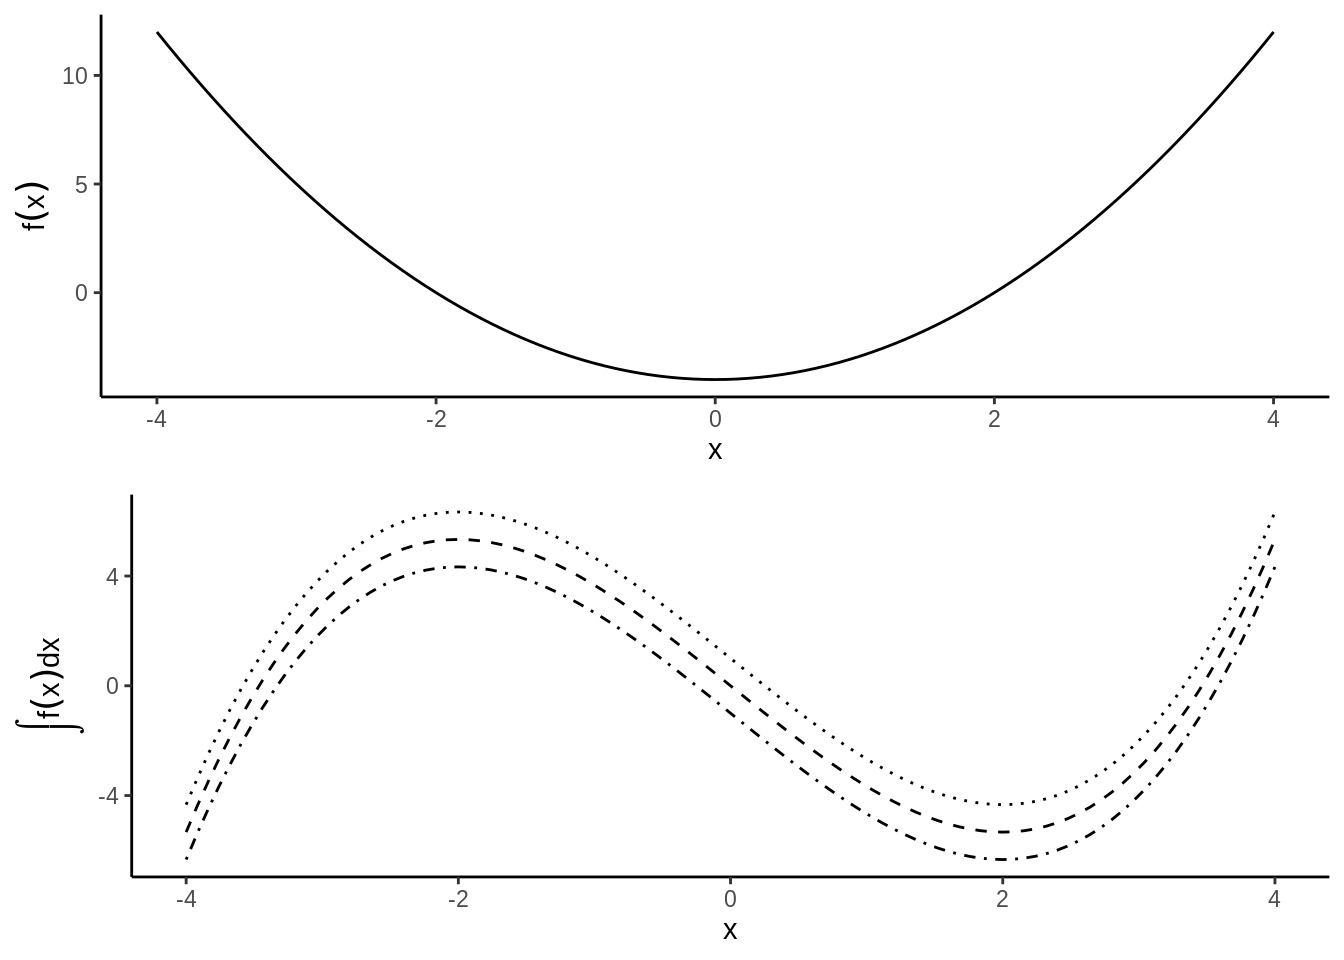
\includegraphics{prefresher_files/figure-latex/integralc-1.pdf}
\caption{\label{fig:integralc}The Many Indefinite Integrals of a Function}
\end{figure}

Notice from these examples that while there is only a single derivative for any function, there are multiple antiderivatives: one for any arbitrary constant \(c\). \(c\) just shifts the curve up or down on the \(y\)-axis. If more information is present about the antiderivative --- e.g., that it passes through a particular point --- then we can solve for a specific value of \(c\).

\hypertarget{common-rules-of-integration}{%
\subsection*{Common Rules of Integration}\label{common-rules-of-integration}}
\addcontentsline{toc}{subsection}{Common Rules of Integration}

Some common rules of integrals follow by virtue of being the inverse of a derivative.

\begin{enumerate}
\def\labelenumi{\arabic{enumi}.}
\tightlist
\item
  Constants are allowed to slip out: \(\int a f(x)dx = a\int f(x)dx\)
\item
  Integration of the sum is sum of integrations: \(\int [f(x)+g(x)]dx=\int f(x)dx + \int g(x)dx\)
\item
  Reverse Power-rule: \(\int x^n dx = \frac{1}{n+1} x^{n+1} + c\)
\item
  Exponents are still exponents: \(\int e^x dx = e^x +c\)
\item
  Recall the derivative of \(\log(x)\) is one over \(x\), and so: \(\int \frac{1}{x} dx = \log x + c\)
\item
  Reverse chain-rule: \(\int e^{f(x)}f^\prime(x)dx = e^{f(x)}+c\)
\item
  More generally: \(\int [f(x)]^n f'(x)dx = \frac{1}{n+1}[f(x)]^{n+1}+c\)
\item
  Remember the derivative of a log of a function: \(\int \frac{f^\prime(x)}{f(x)}dx=\log f(x) + c\)
\end{enumerate}

\BeginKnitrBlock{example}[Common Integration]
\protect\hypertarget{exm:unnamed-chunk-25}{}{\label{exm:unnamed-chunk-25} \iffalse (Common Integration) \fi{} }Simplify the following indefinite integrals:

\begin{itemize}
\tightlist
\item
  \(\int 3x^2 dx\)
\item
  \(\int (2x+1)dx\)
\item
  \(\int e^x e^{e^x} dx\)
\end{itemize}
\EndKnitrBlock{example}

\hypertarget{the-definite-integral-the-area-under-the-curve}{%
\section{The Definite Integral: The Area under the Curve}\label{the-definite-integral-the-area-under-the-curve}}

If there is a indefinite integral, there \emph{must} be a definite integral. Indeed there is, but the notion of definite integrals comes from a different objective: finding the are a under a function. We will find, perhaps remarkably, that the formula we find to get the sum turns out to be expressible by the anti-derivative.

Suppose we want to determine the area \(A(R)\) of a region \(R\) defined by a curve \(f(x)\) and some interval \(a\le x \le b\).

\begin{figure}
\centering
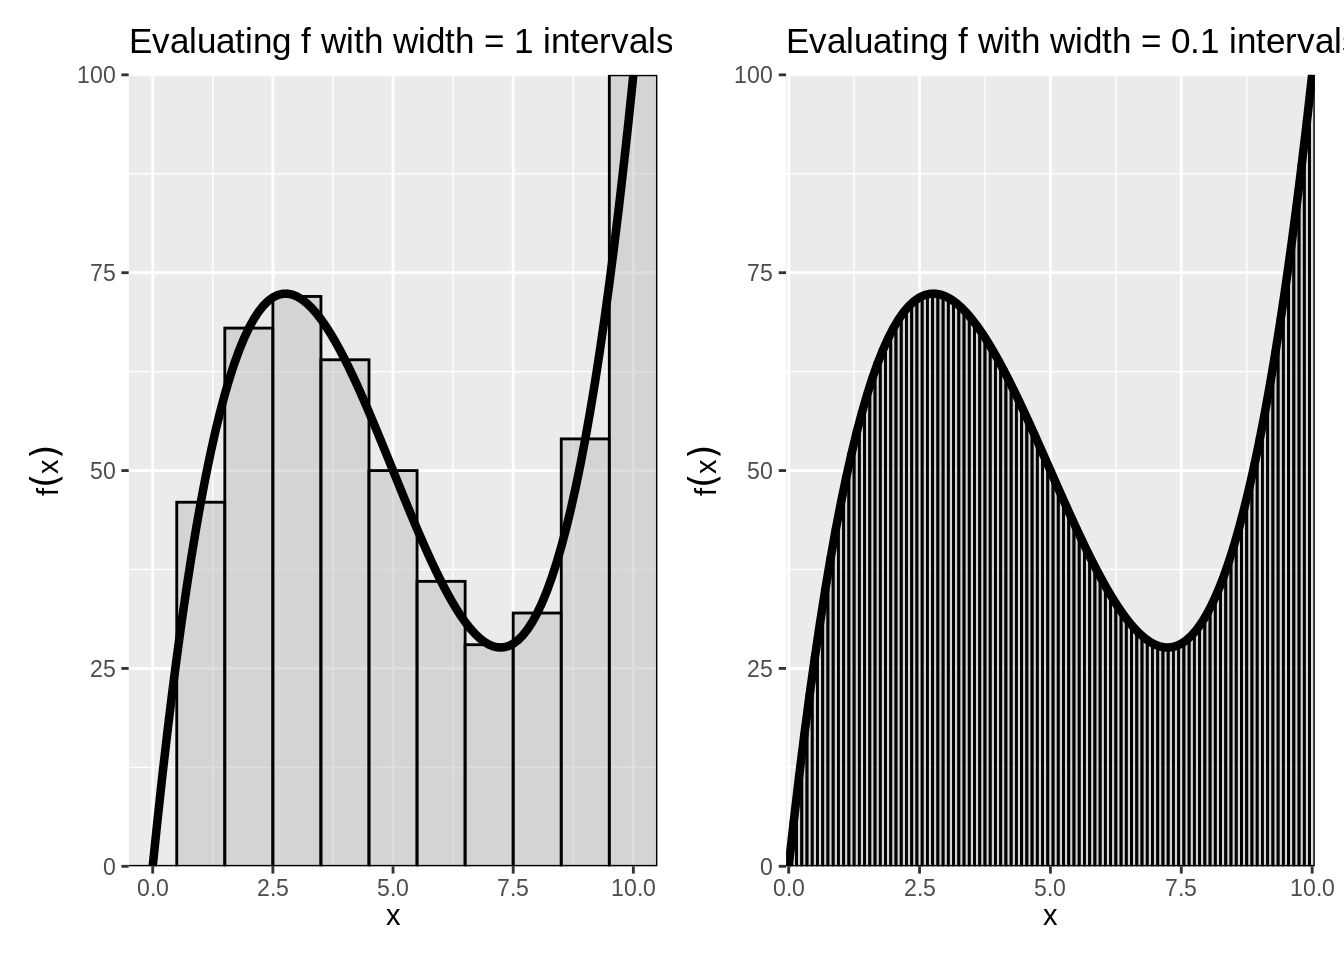
\includegraphics{prefresher_files/figure-latex/defintfig-1.pdf}
\caption{\label{fig:defintfig}The Riemann Integral as a Sum of Evaluations}
\end{figure}

One way to calculate the area would be to divide the interval \(a\le x\le b\) into \(n\) subintervals of length \(\Delta x\) and then approximate the region with a series of rectangles, where the base of each rectangle is \(\Delta x\) and the height is \(f(x)\) at the midpoint of that interval. \(A(R)\) would then be approximated by the area of the union of the rectangles, which is given by \[S(f,\Delta x)=\sum\limits_{i=1}^n f(x_i)\Delta x\] and is called a \textbf{Riemann sum}.

As we decrease the size of the subintervals \(\Delta x\), making the rectangles ``thinner,'' we would expect our approximation of the area of the region to become closer to the true area. This allows us to express the area as a limit of a series:
\[A(R)=\lim\limits_{\Delta x\to 0}\sum\limits_{i=1}^n f(x_i)\Delta x\]

Figure \ref{fig:defintfig} shows that illustration. The curve depicted is \(f(x) = -15(x - 5) + (x - 5)^3 + 50.\) We want approximate the area under the curve between the \(x\) values of 0 and 10. We can do this in blocks of arbitrary width, where the sum of rectangles (the area of which is width times \(f(x)\) evaluated at the midpoint of the bar) shows the Riemann Sum. As the width of the bars \(\Delta x\) becomes smaller, the better the estimate of \(A(R)\).

This is how we define the ``Definite'' Integral:

\BeginKnitrBlock{definition}[The Definite Integral (Riemann)]
\protect\hypertarget{def:unnamed-chunk-26}{}{\label{def:unnamed-chunk-26} \iffalse (The Definite Integral (Riemann)) \fi{} }If for a given function \(f\) the Riemann sum approaches a limit as \(\Delta x \to 0\), then that limit is called the Riemann integral of \(f\) from \(a\) to \(b\). We express this with the \(\int\), symbol, and write \[\int\limits_a^b f(x) dx= \lim\limits_{\Delta x\to 0} \sum\limits_{i=1}^n f(x_i)\Delta x\]

The most straightforward of a definite integral is the definite integral. That is, we read
\[\int\limits_a^b f(x) dx\] as the definite integral of \(f\) from \(a\) to \(b\) and we defined as the area under the ``curve'' \(f(x)\) from point \(x=a\) to \(x=b\).
\EndKnitrBlock{definition}

The fundamental theorem of calculus shows us that this sum is, in fact, the antiderivative.

\BeginKnitrBlock{theorem}[First Fundamental Theorem of Calculus]
\protect\hypertarget{thm:unnamed-chunk-27}{}{\label{thm:unnamed-chunk-27} \iffalse (First Fundamental Theorem of Calculus) \fi{} }Let the function \(f\) be bounded on \([a,b]\) and continuous on \((a,b)\). Then, suggestively, use the symbol \(F(x)\) to denote the definite integral from \(a\) to \(x\):
\[F(x)=\int\limits_a^x f(t)dt, \quad a\le x\le b\]

Then \(F(x)\) has a derivative at each point in \((a,b)\) and \[F^\prime(x)=f(x), \quad a<x<b\]
That is, the definite integral function of \(f\) \emph{is} the one of the antiderivatives of some \(f\).
\EndKnitrBlock{theorem}

This is again a long way of saying that that differentiation is the inverse of integration. But now, we've covered definite integrals.

The second theorem gives us a simple way of computing a definite integral as a function of indefinite integrals.

\BeginKnitrBlock{theorem}[Second Fundamental Theorem of Calculus]
\protect\hypertarget{thm:unnamed-chunk-28}{}{\label{thm:unnamed-chunk-28} \iffalse (Second Fundamental Theorem of Calculus) \fi{} }Let the function \(f\) be bounded on \([a,b]\) and continuous on \((a,b)\). Let \(F\) be any function that is continuous on \([a,b]\) such that \(F^\prime(x)=f(x)\) on \((a,b)\). Then \[\int\limits_a^bf(x)dx = F(b)-F(a)\]
\EndKnitrBlock{theorem}

So the procedure to calculate a simple definite integral \(\int\limits_a^b f(x)dx\) is then

\begin{enumerate}
\def\labelenumi{\arabic{enumi}.}
\tightlist
\item
  Find the indefinite integral \(F(x)\).
\item
  Evaluate \(F(b)-F(a)\).
\end{enumerate}

\BeginKnitrBlock{example}[Definite Integral of a monomial]
\protect\hypertarget{exm:defintmon}{}{\label{exm:defintmon} \iffalse (Definite Integral of a monomial) \fi{} }Solve \(\int\limits_1^3 3x^2 dx.\)

Let \(f(x) = 3x^2\).
\EndKnitrBlock{example}

\BeginKnitrBlock{exercise}
\protect\hypertarget{exr:unnamed-chunk-29}{}{\label{exr:unnamed-chunk-29} }What is the value of \(\int\limits_{-2}^2 e^x e^{e^x} dx\)?
\EndKnitrBlock{exercise}

\hypertarget{common-rules-for-definite-integrals}{%
\subsection*{Common Rules for Definite Integrals}\label{common-rules-for-definite-integrals}}
\addcontentsline{toc}{subsection}{Common Rules for Definite Integrals}

The area-interpretation of the definite integral provides some rules for simplification.

\begin{enumerate}
\def\labelenumi{\arabic{enumi}.}
\tightlist
\item
  There is no area below a point: \[\int\limits_a^a f(x)dx=0\]
\item
  Reversing the limits changes the sign of the integral: \[\int\limits_a^b f(x)dx=-\int\limits_b^a f(x)dx\]
\item
  Sums can be separated into their own integrals: \[\int\limits_a^b [\alpha f(x)+\beta g(x)]dx = \alpha \int\limits_a^b f(x)dx + \beta \int\limits_a^b g(x)dx\]
\item
  Areas can be combined as long as limits are linked: \[\int\limits_a^b f(x) dx +\int\limits_b^c f(x)dx = \int\limits_a^c f(x)dx\]
\end{enumerate}

\BeginKnitrBlock{exercise}[Definite integral shortcuts]
\protect\hypertarget{exr:unnamed-chunk-30}{}{\label{exr:unnamed-chunk-30} \iffalse (Definite integral shortcuts) \fi{} }Simplify the following definite intergrals.

\begin{enumerate}
\def\labelenumi{\arabic{enumi}.}
\tightlist
\item
  \(\int\limits_1^1 3x^2 dx =\)
\item
  \(\int\limits_0^4 (2x+1)dx=\)
\item
  \(\int\limits_{-2}^0 e^x e^{e^x} dx + \int\limits_0^2 e^x e^{e^x} dx =\)
\end{enumerate}
\EndKnitrBlock{exercise}

\hypertarget{integration-by-substitution}{%
\section{Integration by Substitution}\label{integration-by-substitution}}

From the second fundamental theorem of calculus, we now that a quick way to get a definite integral is to first find the indefinite integral, and then just plug in the bounds.

Sometimes the integrand (the thing that we are trying to take an integral of) doesn't appear integrable using common rules and antiderivatives. A method one might try is \textbf{integration by substitution}, which is related to the Chain Rule.

Suppose we want to find the indefinite integral \[\int g(x)dx\] but \(g(x)\) is complex and none of the formulas we have seen so far seem to apply immediately. The trick is to come up with a \emph{new} function \(u(x)\) such that \[g(x)=f[u(x)]u'(x).\]

Why does an introduction of yet another function end of simplifying things? Let's refer to the antiderivative of \(f\) as \(F\). Then the chain rule tells us that \[\frac{d}{dx} F[u(x)]=f[u(x)]u'(x)\]. So, \(F[u(x)]\) is the antiderivative of \(g\). We can then write \[\int g(x) dx= \int f[u(x)]u'(x)dx = \int \frac{d}{dx} F[u(x)]dx = F[u(x)]+c\]

To summarize, the procedure to determine the indefinite integral \(\int g(x)dx\) by the method of substitution:

\begin{enumerate}
\def\labelenumi{\arabic{enumi}.}
\tightlist
\item
  Identify some part of \(g(x)\) that might be simplified by substituting in a single variable \(u\) (which will then be a function of \(x\)).
\item
  Determine if \(g(x)dx\) can be reformulated in terms of \(u\) and \(du\).
\item
  Solve the indefinite integral.
\item
  Substitute back in for \(x\)
\end{enumerate}

Substitution can also be used to calculate a definite integral. Using the same procedure as above, \[\int\limits_a^b g(x)dx=\int\limits_c^d f(u)du = F(d)-F(c)\]
where \(c=u(a)\) and \(d=u(b)\).

\BeginKnitrBlock{example}[Integration by Substitution I]
\protect\hypertarget{exm:intsub1}{}{\label{exm:intsub1} \iffalse (Integration by Substitution I) \fi{} }
Solve the indefinite integral \[\int x^2 \sqrt{x+1}dx.\]
\EndKnitrBlock{example}

For the above problem, we could have also used the substitution \(u=\sqrt{x+1}\). Then \(x=u^2-1\) and \(dx=2u du\). Substituting these in, we get \[\int x^2\sqrt{x+1}dx=\int (u^2-1)^2 u 2u du\] which when expanded is again a polynomial and gives the same result as above.

Another case in which integration by substitution is is useful is with a fraction.

\BeginKnitrBlock{example}[Integration by Substitutiton II]
\protect\hypertarget{exm:intsub2}{}{\label{exm:intsub2} \iffalse (Integration by Substitutiton II) \fi{} }Simplify \[\int\limits_0^1 \frac{5e^{2x}}{(1+e^{2x})^{1/3}}dx.\]
\EndKnitrBlock{example}

\hypertarget{integration-by-parts}{%
\section{Integration by Parts}\label{integration-by-parts}}

Another useful integration technique is \textbf{integration by parts}, which is related to the Product Rule of differentiation. The product rule states that \[\frac{d}{dx}(uv)=u\frac{dv}{dx}+v\frac{du}{dx}\] Integrating this and rearranging, we get \[\int u\frac{dv}{dx}dx= u v - \int v \frac{du}{dx}dx\] or \[\int u(x) v'(x)dx=u(x)v(x) - \int v(x)u'(x)dx\]

More easily remembered with the mnemonic ``Ultraviolet Voodoo'': \[\int u dv = u v - \int v du\] where \(du=u'(x)dx\) and \(dv=v'(x)dx\).

For definite integrals, this is simply
\[\int\limits_a^b u\frac{dv}{dx}dx = \left. u v \right|_a^b - \int\limits_a^b v \frac{du}{dx}dx\]

Our goal here is to find expressions for \(u\) and \(dv\) that, when substituted into the above equation, yield an expression that's more easily evaluated.

\BeginKnitrBlock{example}[Integration by Parts]
\protect\hypertarget{exm:unnamed-chunk-31}{}{\label{exm:unnamed-chunk-31} \iffalse (Integration by Parts) \fi{} }Simplify the following integrals. These seemingly obscure forms of integrals come up often when integrating distributions.

\[\int x e^{ax} dx\]
\EndKnitrBlock{example}

\BeginKnitrBlock{solution}
\iffalse{} {Solution. } \fi{}
Let \(u=x\) and \(\frac{dv}{dx} = e^{ax}\). Then \(du=dx\) and \(v=(1/a)e^{ax}\). Substituting this into the integration by parts formula, we obtain\\
\begin{eqnarray}
\int x e^{ax} dx &=& u v - \int v du\nonumber\\
                &=&x\left( \frac{1}{a}e^{ax}\right) -\int\frac{1}{a}e^{ax}dx\nonumber\\
                &=&\frac{1}{a}xe^{ax}-\frac{1}{a^2}e^{ax}+c\nonumber
\end{eqnarray}
\EndKnitrBlock{solution}

\BeginKnitrBlock{exercise}[Integration by Parts II]
\protect\hypertarget{exr:intparts-adv}{}{\label{exr:intparts-adv} \iffalse (Integration by Parts II) \fi{} }
1. Integrate
\[\int x^n e^{ax} dx\]

\begin{enumerate}
\def\labelenumi{\arabic{enumi}.}
\setcounter{enumi}{1}
\tightlist
\item
  Integrate
  \[\int x^3 e^{-x^2} dx\]
\end{enumerate}
\EndKnitrBlock{exercise}

\hypertarget{answers-to-examples-and-exercises-2}{%
\section*{Answers to Examples and Exercises}\label{answers-to-examples-and-exercises-2}}
\addcontentsline{toc}{section}{Answers to Examples and Exercises}

Exercise \ref{exr:introderivatives}

\BeginKnitrBlock{solution}
\iffalse{} {Solution. } \fi{}

\begin{enumerate}
\def\labelenumi{\arabic{enumi}.}
\tightlist
\item
  \(f^\prime(x)= 0\)
\item
  \(f^\prime(x)= 1\)
\item
  \(f^\prime(x)= 2x^3\)
\item
  \(f\prime(x)= 3x^2\)
\item
  \(f\prime(x)= -2x^{-3}\)
\item
  \(f\prime(x)= 14x^6\)
\item
  \(f\prime(x) = 4x^3 - 3x^2 + 2x -1\)
\item
  \(f\prime(x) = 5x^4 + 3x^2 - 2x\)
\item
  \(f\prime(x) = 6x + \frac{2}{3}x^{\frac{-2}{3}}\)
\item
  \(f\prime(x)= \frac{-4x}{x^4 - 2x^2 + 1}\)
\end{enumerate}
\EndKnitrBlock{solution}

Example \ref{exm:tothesix}

\BeginKnitrBlock{solution}
\iffalse{} {Solution. } \fi{}For convenience, define \(f(z) = z^6\) and \(z = g(x) = 3x^2+5x-7\). Then, \(y=f[g(x)]\) and

\begin{align*}
\frac{d}{dx}y&= f^\prime(z) g^\prime(x) \\
&= 6(3x^2+5x-7)^5 (6x + 5)
\end{align*}
\EndKnitrBlock{solution}

Example \ref{exm:exmderivexp}

\BeginKnitrBlock{solution}
\iffalse{} {Solution. } \fi{}

\begin{enumerate}
\def\labelenumi{\arabic{enumi}.}
\tightlist
\item
  Let \(u(x)=-3x\). Then \(u^\prime(x)=-3\) and \(f^\prime(x)=-3e^{-3x}\).
\item
  Let \(u(x)=x^2\). Then \(u^\prime(x)=2x\) and \(f^\prime(x)=2xe^{x^2}\).
\end{enumerate}
\EndKnitrBlock{solution}

Example \ref{exm:exmderivlog}

\BeginKnitrBlock{solution}
\iffalse{} {Solution. } \fi{}

\begin{enumerate}
\def\labelenumi{\arabic{enumi}.}
\tightlist
\item
  Let \(u(x)=x^2+9\). Then \(u^\prime(x)=2x\) and \[\frac{dy}{dx}= \frac{u^\prime(x)}{u(x)} = \frac{2x}{(x^2+9)}\]
\item
  Let \(u(x)=\log x\). Then \(u^\prime(x)=1/x\) and \(\frac{dy}{dx} = \frac{1}{(x\log x)}\).
\item
  Use the generalized power rule. \[\frac{dy}{dx} = \frac{(2 \log x)}{x}\]
\item
  We know that \(\log e^x=x\) and that \(dx/dx=1\), but we can double check. Let \(u(x)=e^x\). Then \(u^\prime(x)=e^x\) and \(\frac{dy}{dx} = \frac{u^\prime(x)}{u(x)} = \frac{e^x}{e^x} = 1.\)
\end{enumerate}
\EndKnitrBlock{solution}

Example \ref{exm:defintmon}

\BeginKnitrBlock{solution}
\iffalse{} {Solution. } \fi{}What is \(F(x)\)? From the power rule, recognize \(\frac{d}{dx}x^3 = 3x^2\) so

\begin{align*}
F(x) &= x^3\\
\int\limits_1^3 f(x) dx &= F(x = 3) - F(x  - 1)\\
&= 3^3 - 1^3\\
&=26
\end{align*}
\EndKnitrBlock{solution}

Example \ref{exm:intsub1}
\BeginKnitrBlock{solution}
\iffalse{} {Solution. } \fi{}The problem here is the \(\sqrt{x+1}\) term. However, if the integrand had \(\sqrt{x}\) times some polynomial, then we'd be in business. Let's try \(u=x+1\). Then \(x=u-1\) and \(dx=du\). Substituting these into the above equation, we get

\begin{align*}
            \int x^2\sqrt{x+1}dx&= \int (u-1)^2\sqrt{u}du\\
            &= \int (u^2-2u+1)u^{1/2}du\\
            &= \int (u^{5/2}-2u^{3/2}+u^{1/2})du
\end{align*}

We can easily integrate this, since it is just a polynomial. Doing so and substituting \(u=x+1\) back in, we get \[\int x^2\sqrt{x+1}dx=2(x+1)^{3/2}\left[\frac{1}{7}(x+1)^2 -
\frac{2}{5}(x+1)+\frac{1}{3}\right]+c\]
\EndKnitrBlock{solution}

Example \ref{exm:intsub2}
\BeginKnitrBlock{solution}
\iffalse{} {Solution. } \fi{}When an expression is raised to a power, it is often helpful to use this expression as the basis for a substitution. So, let \(u=1+e^{2x}\). Then \(du=2e^{2x}dx\) and we can set \(5e^{2x}dx=5du/2\). Additionally, \(u=2\) when \(x=0\) and \(u=1+e^2\) when \(x=1\). Substituting all of this in, we get

\begin{align*}
\int\limits_0^1 \frac{5e^{2x}}{(1+e^{2x})^{1/3}}dx
            &= \frac{5}{2}\int\limits_2^{1+e^2}\frac{du}{u^{1/3}}\\
            &= \frac{5}{2}\int\limits_2^{1+e^2} u^{-1/3}du\\
            &= \left. \frac{15}{4} u^{2/3} \right|_2^{1+e^2}\\
            &= 9.53
\end{align*}
\EndKnitrBlock{solution}

Exercise \ref{exr:intparts-adv}

1. \[\int x^n e^{ax} dx\]
\BeginKnitrBlock{solution}
\iffalse{} {Solution. } \fi{}
As in the first problem, let
\[u=x^n, dv=e^{ax}dx\]
Then \(du=n x^{n-1}dx\) and \(v=(1/a)e^{ax}\).

Substituting these into the integration by parts formula gives
\begin{eqnarray}
            \int x^n e^{ax} dx &=& u v - \int v du\nonumber\\
            &=&x^n\left( \frac{1}{a}e^{ax}\right) - \int\frac{1}{a}e^{ax} n x^{n-1} dx\nonumber\\
            &=&\frac{1}{a}x^n e^{ax} - \frac{n}{a}\int x^{n-1}e^{ax}dx\nonumber
\end{eqnarray}

Notice that we now have an integral similar to the previous one, but with \(x^{n-1}\) instead of \(x^n\).

For a given \(n\), we would repeat the integration by parts procedure until the integrand was directly integratable --- e.g., when the integral became \(\int e^{ax}dx\).
\EndKnitrBlock{solution}

2. \[\int x^3 e^{-x^2} dx\]

\BeginKnitrBlock{solution}
\iffalse{} {Solution. } \fi{}We could, as before, choose \(u=x^3\) and \(dv=e^{-x^2}dx\). But we can't then find \(v\) --- i.e., integrating \(e^{-x^2}dx\) isn't possible. Instead, notice that \[\frac{d}{dx}e^{-x^2} = -2xe^{-x^2},\] which can be factored out of the original integrand \[\int x^3 e^{-x^2} dx = \int x^2 (xe^{-x^2})dx.\]

We can then let \(u=x^2\) and \(dv=x e^{-x^2}dx\). The\(du=2x dx\) and \(v=-\frac{1}{2}e^{-x^2}\). Substituting these in, we have
\begin{eqnarray}
                \int x^3 e^{-x^2} dx &=& u v - \int v du\nonumber\\
                &=& x^2 \left( -\frac{1}{2}e^{-x^2}\right) -\int \left(-\frac{1}{2}e^{-x^2}\right)2x dx\nonumber\\
                &=& -\frac{1}{2}x^2 e^{-x^2}+\int x e^{-x^2}dx\nonumber\\
                &=& -\frac{1}{2}x^2 e^{-x^2}-\frac{1}{2}e^{-x^2}+c\nonumber
\end{eqnarray}
\EndKnitrBlock{solution}

\hypertarget{optim}{%
\chapter{Optimization}\label{optim}}

To optimize, we use derivatives and calculus. Optimization is to find the maximum or minimum of a functon, and to find what value of an input gives that extremum. This has obvious uses in engineering. Many tools in the statistical toolkit use optimization. One of the most common ways of estimating a model is through ``Maximum Likelihood Estimation'', done via optimizing a function (the likelihood).

Optimization also comes up in Economics, Formal Theory, and Political Economy all the time. A go-to model of human behavior is that they optimize a certain utility function. Humans are not pure utility maximizers, of course, but nuanced models of optimization -- for example, adding constraints and adding uncertainty -- will prove to be quite useful.

\hypertarget{example-meltzer-richard}{%
\section*{Example: Meltzer-Richard}\label{example-meltzer-richard}}
\addcontentsline{toc}{section}{Example: Meltzer-Richard}

A standard backdrop in comparative political economy, the Meltzer-Richard (1981) model states that redistribution of wealth should be higher in societies where the median income is much smaller than the average income. More to the point, typically income distributions wher ethe median is very different from the average is one of high inequality. In other words, the Meltzer-Richard model says that highly unequal economies will have more re-distribution of wealth. Why is that the case? Here is a simplified example that is not the exact model by Meltzer and Richard\footnote{Allan H. Meltzer and Scott F. Richard. \href{https://www.jstor.org/stable/1830813}{``A Rational Theory of the Size of Government''}. \emph{Journal of Political Economy}
  89:5 (1981), p.~914-927}, but adapted from Persson and Tabellini\footnote{Adapted from Torsten Persson and Guido Tabellini, \emph{Political Economics: Explaining Economic Policy}. MIT Press. }

We will set the following things about our model human and model democracy.

\begin{itemize}
\tightlist
\item
  Individuals are indexed by \(i\), and the total population is normalized to unity (``1'') without loss of generality.
\item
  \(U(\cdot)\), u for ``utility'', is a function that is concave and increasing, and expresses the utility gained from public goods. This tells us that its first derivative is \emph{positive}, and its second derivative is \textbf{negative}.
\item
  \(y_i\) is the income of person \(i\)
\item
  \(W_i\), w for ``welfare'', is the welfare of person \(i\)
\item
  \(c_i\), c for ``consumption'', is the consumption utility of person \(i\)
\end{itemize}

Also, the government is democratically elected and sets the following redistribution output:

\begin{itemize}
\tightlist
\item
  \(\tau\), t for ``tax'', is a flat tax rate between 0 and 1 that is applied to everyone's income.
\item
  \(g\), ``g'' for ``goods'', is the amount of public goods that the government provides.
\end{itemize}

Suppose an individual's welfare is given by:
\[W_i = c_i + U(g)\]

The consumption good is the person's post-tax income.

\[c_i = (1 - \tau) y_i\]

Income varies by person (In the next section we will cover probability, by then we will know that we can express this by saying that \(y\) is a random variable with the cumulative distribution function \(F\), i.e. \(y \sim F\).). Every distribution has a mean and an median.

\begin{itemize}
\tightlist
\item
  \(E(y)\) is the average income of the society.
\item
  \(\text{med}(y)\) is the \textbf{median income} of the society.
\end{itemize}

What will happen in this economy? What will the tax rate be set too? How much public goods will be provided?

We've skipped ahead of some formal theory results of demoracy, but hopefully these are conceptually intuitive. First, if a democracy is competitive, there is no slack in the government's goods, and all tax revenue becomes a public good. So we can go ahead and set the constraint:

\[g = \sum_{i} \tau y_i P(y_i) = \tau E(y)\]

We can do this trick because of the ``normalizes to unity'' setting, but this is a general property of the average.

Now given this constraint we can re-write an individual's welfare as

\begin{align*}
W_i &= \left(1 - \frac{g}{E(y)}\right)y_i + U(g)\\
&= \left(E(y) - g\right) \frac{1}{E(y)} y_i + U(g)\\
&= \left(E(y) - g\right) \frac{y_i}{E(y)} + U(g)\\
\end{align*}

When is the individual's welfare maximized, \textbf{as a function of the public good}?
\begin{align*}
\frac{d}{dg}W_i &=  - \frac{y_i}{E(y)} + \frac{d}{dg}U(g)\\
\end{align*}

\(\frac{d}{dg}W_i = 0\) when \(\frac{d}{dg}U(g) = \frac{y_i}{E(y)}\), and so after expressing the derivative as \(U_g = \frac{d}{dg}U(g)\) for simplicity,

\[g_i^\star = {U_g}^{-1}\left(\frac{y_i}{E(y)}\right)\]

Now recall that because we assumed concavity, \(U_g\) is a negative sloping function whose value is positive. It can be shown that the inverse of such a function is also decreasing. Thus an individual's preferred level of government is determined by a single continuum, the person's income divided by the average income, and the function is \textbf{decreasing} in \(y_i\). This is consistent with our intuition that richer people prefer less redistribution.

That was the amount for any given person. The government has to set one value of \(g\), however. So what will that be? Now we will use another result, the median voter theorem. This says that under certain general electoral conditions (single-peaked preferences, two parties, majority rule), the policy winner will be that preferred by the median person in the population. Because the only thing that determines a person's preferred level of government is \(y_i / E(y)\), we can presume that the median voter, whose income is \(\text{med}(y)\) will prevail in their preferred choice of government. Therefore, we wil see

\[g^\star = {U_g}^{-1}\left(\frac{\text{med}(y)}{E(y)}\right)\]

What does this say about the level of redistribution we observe in an economy? The higher the average income is than the median income, which often (but not always) means \emph{more} inequality, there should be \emph{more} redistribution.

\hypertarget{maxima-and-minima}{%
\section{Maxima and Minima}\label{maxima-and-minima}}

The first derivative, \(f'(x)\), quantifies the slope of a function. Therefore, it can be used to check whether the function \(f(x)\) at the point \(x\) is increasing or decreasing at \(x\).

\begin{enumerate}
\def\labelenumi{\arabic{enumi}.}
\tightlist
\item
  \textbf{Increasing:} \(f'(x)>0\)
\item
  \textbf{Decreasing:} \(f'(x)<0\)
\item
  \textbf{Neither increasing nor decreasing}: \(f'(x)=0\)
  i.e.~a maximum, minimum, or saddle point
\end{enumerate}

So for example, \(f(x) = x^2 + 2\) and \(f^\prime(x) = 2x\)

\begin{figure}
\centering
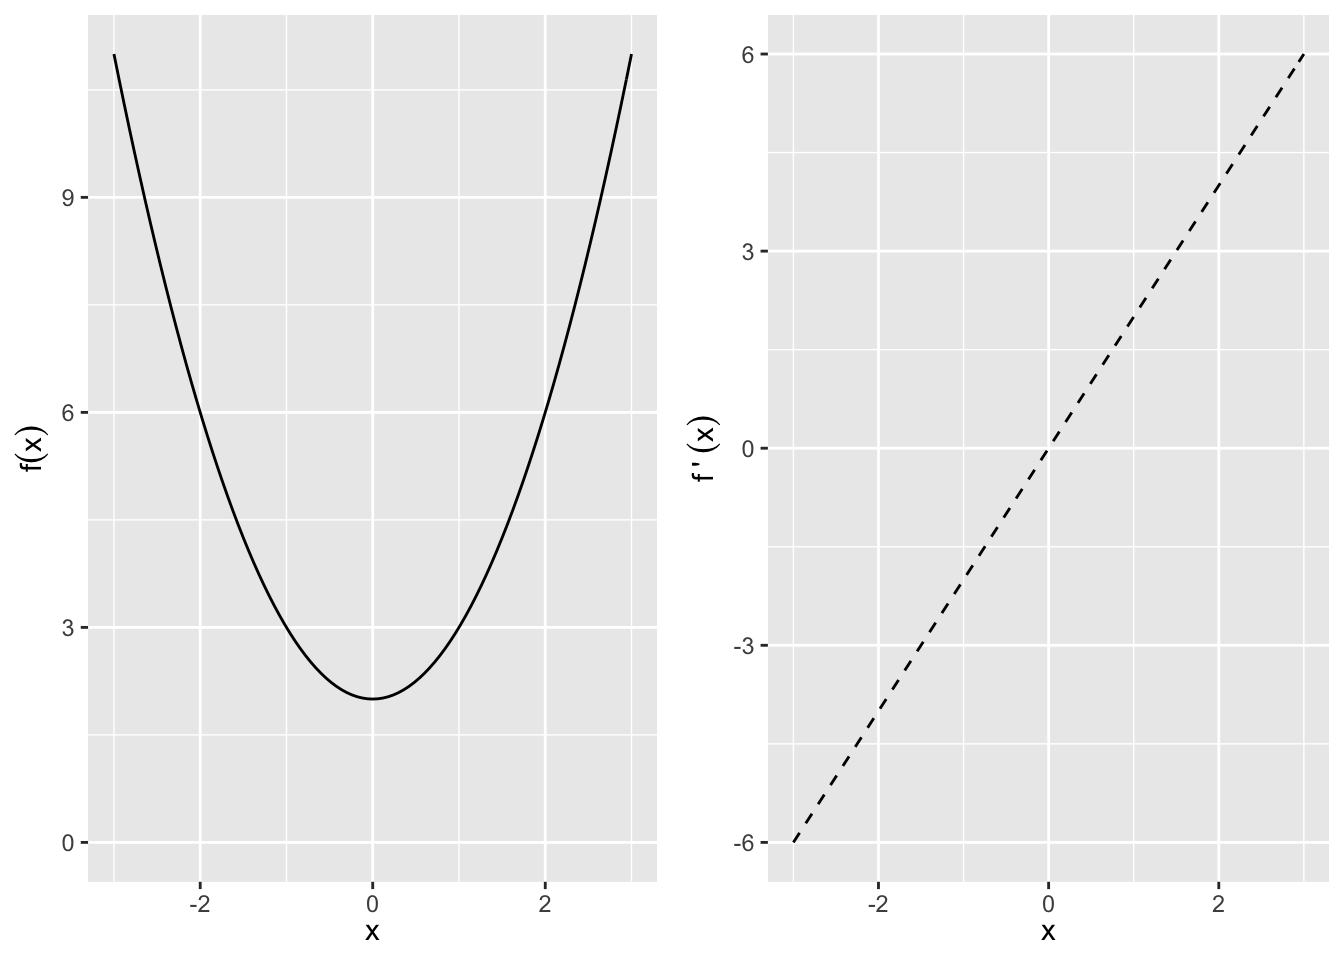
\includegraphics{prefresher_files/figure-latex/unnamed-chunk-43-1.pdf}
\caption{\label{fig:unnamed-chunk-43}Maxima and Minima}
\end{figure}

\BeginKnitrBlock{exercise}[Plotting a mazimum and minimum]
\protect\hypertarget{exr:unnamed-chunk-44}{}{\label{exr:unnamed-chunk-44} \iffalse (Plotting a mazimum and minimum) \fi{} }Plot \(f(x)=x^3+ x^2 + 2\), plot its derivative, and identifiy where the derivative is zero. Is there a maximum or minimum?
\EndKnitrBlock{exercise}

The second derivative \(f''(x)\) identifies whether the function \(f(x)\) at the point \(x\) is

\begin{enumerate}
\def\labelenumi{\arabic{enumi}.}
\tightlist
\item
  Concave down: \(f''(x)<0\)
\item
  Concave up: \(f''(x)>0\)
\end{enumerate}

\textbf{Maximum (Minimum)}: \(x_0\) is a \textbf{local maximum (minimum)} if \(f(x_0)>f(x)\) (\(f(x_0)<f(x))\) for all \(x\) within some open interval containing \(x_0\). \(x_0\) is a \textbf{global maximum (minimum)} if \(f(x_0)>f(x)\) (\(f(x_0)<f(x))\) for all \(x\) in the domain of \(f\).

Given the function \(f\) defined over domain \(D\), all of the following are defined as \textbf{critical points}:

\begin{enumerate}
\def\labelenumi{\arabic{enumi}.}
\tightlist
\item
  Any interior point of \(D\) where \(f'(x)=0\).
\item
  Any interior point of \(D\) where \(f'(x)\) does not exist.
\item
  Any endpoint that is in \(D\).
\end{enumerate}

The maxima and minima will be a subset of the critical points.

\textbf{Second Derivative Test of Maxima/Minima}: We can use the second derivative to tell us whether a point is a maximum or minimum of \(f(x)\).

\begin{enumerate}
\def\labelenumi{\arabic{enumi}.}
\tightlist
\item
  Local Maximum: \(f'(x)=0\) and \(f''(x)<0\)
\item
  Local Minimum: \(f'(x)=0\) and \(f''(x)>0\)
\item
  Need more info: \(f'(x)=0\) and \(f''(x)=0\)
\end{enumerate}

\textbf{Global Maxima and Minima} Sometimes no global max or min exists --- e.g., \(f(x)\) not bounded above or below. However, there are three situations where we can fairly easily identify global max or min.

\begin{enumerate}
\def\labelenumi{\arabic{enumi}.}
\tightlist
\item
  \textbf{Functions with only one critical point.} If \(x_0\) is a local max or min of \(f\) and it is the only critical point, then it is the global max or min.
\item
  \textbf{Globally concave up or concave down functions.} If \(f''(x)\) is never zero, then there is at most one critical point. That critical point is a global maximum if \(f''<0\) and a global minimum if \(f''>0\).
\item
  \textbf{Functions over closed and bounded intervals} must have both a global maximum and a global minimum.
\end{enumerate}

\BeginKnitrBlock{example}[Maxima and Minima by drawing]
\protect\hypertarget{exm:unnamed-chunk-46}{}{\label{exm:unnamed-chunk-46} \iffalse (Maxima and Minima by drawing) \fi{} }
Find any critical points and identify whether they are a max, min, or saddle point:

\begin{enumerate}
\def\labelenumi{\arabic{enumi}.}
\tightlist
\item
  \(f(x)=x^2+2\)
\item
  \(f(x)=x^3+2\)
\item
  \(f(x)=|x^2-1|\), \(x\in [-2,2]\)
\end{enumerate}
\EndKnitrBlock{example}

\hypertarget{concavity-of-a-function}{%
\section{Concavity of a Function}\label{concavity-of-a-function}}

Concavity helps identify the curvature of a function, \(f(x)\), in 2 dimensional space.

\BeginKnitrBlock{definition}[Concave Function]
\protect\hypertarget{def:unnamed-chunk-47}{}{\label{def:unnamed-chunk-47} \iffalse (Concave Function) \fi{} }A function \(f\) is strictly concave over the set S \underline{if} \(\forall x_1,x_2 \in S\) and \(\forall a \in (0,1)\), \[f(ax_1 + (1-a)x_2) > af(x_1) + (1-a)f(x_2)\]
\textit{Any} line connecting two points on a concave function will lie \textit{below} the function.
\EndKnitrBlock{definition}

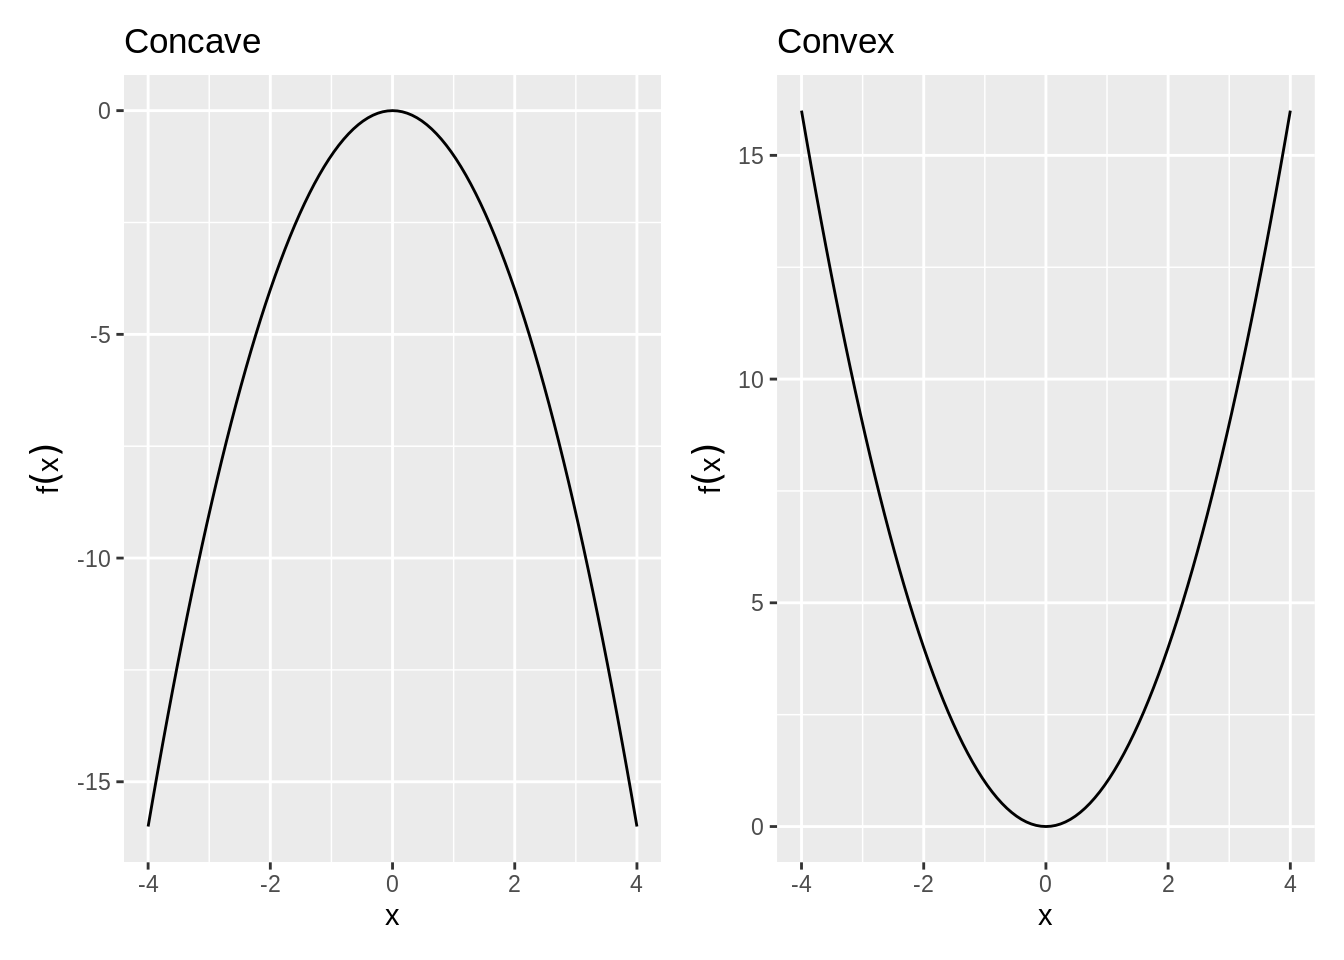
\includegraphics{prefresher_files/figure-latex/unnamed-chunk-48-1.pdf}

\BeginKnitrBlock{definition}[Convex Function]
\protect\hypertarget{def:unnamed-chunk-49}{}{\label{def:unnamed-chunk-49} \iffalse (Convex Function) \fi{} }Convex: A function f is strictly convex over the set S \underline{if} \(\forall x_1,x_2 \in S\) and \(\forall a \in (0,1)\), \[f(ax_1 + (1-a)x_2) < af(x_1) + (1-a)f(x_2)\]

Any line connecting two points on a convex function will lie above the function.
\EndKnitrBlock{definition}

\begin{comment}
  \parbox{2in}{\includegraphics[scale=.4]{Convex.pdf}}
\end{comment}

Sometimes, concavity and convexity are strict of a requirement. For most purposes of getting solutions, what we call quasi-concavity is enough.

\BeginKnitrBlock{definition}[Quasiconcave Function]
\protect\hypertarget{def:unnamed-chunk-50}{}{\label{def:unnamed-chunk-50} \iffalse (Quasiconcave Function) \fi{} }A function f is quasiconcave over the set S if \(\forall x_1,x_2 \in S\) and \(\forall a \in (0,1)\), \[f(ax_1 + (1-a)x_2) \ge \min(f(x_1),f(x_2))\]

No matter what two points you select, the \textit{lowest} valued point will always be an end point.
\EndKnitrBlock{definition}

\begin{comment}
  \parbox{2in}{\includegraphics[scale=.4]{Quasiconcave.pdf}}
\end{comment}

\BeginKnitrBlock{definition}[Quasiconvex]
\protect\hypertarget{def:unnamed-chunk-51}{}{\label{def:unnamed-chunk-51} \iffalse (Quasiconvex) \fi{} }A function f is quasiconvex over the set \(S\) if \(\forall x_1,x_2 \in S\) and \(\forall a \in (0,1)\), \[f(ax_1 + (1-a)x_2) \le \max(f(x_1),f(x_2))\]
No matter what two points you select, the \textit{highest} valued point will always be an end point.
\EndKnitrBlock{definition}

\begin{comment}
  \parbox{1.8in}{\includegraphics[scale=.4]{Quasiconvex.pdf}}
\end{comment}

\textbf{Second Derivative Test of Concavity}: The second derivative can be used to understand concavity.

If
\[\begin{array}{lll}
f''(x) < 0 & \Rightarrow & \text{Concave}\\
f''(x) > 0 & \Rightarrow & \text{Convex}
\end{array}\]

\hypertarget{quadratic-forms}{%
\subsection*{Quadratic Forms}\label{quadratic-forms}}
\addcontentsline{toc}{subsection}{Quadratic Forms}

Quadratic forms is shorthand for a way to summarize a function. This is important for finding concavity because

\begin{enumerate}
\def\labelenumi{\arabic{enumi}.}
\tightlist
\item
  Approximates local curvature around a point --- e.g., used to
  identify max vs min vs saddle point.
\item
  They are simple to express even in \(n\) dimensions:
\item
  Have a matrix representation.
\end{enumerate}

\textbf{Quadratic Form}: A polynomial where each term is a monomial
of degree 2 in any number of variables:

\begin{align*}
\text{One variable: }& Q(x_1) = a_{11}x_1^2\\
\text{Two variables: }& Q(x_1,x_2) = a_{11}x_1^2 + a_{12}x_1x_2 + a_{22}x_2^2\\
\text{N variables: }& Q(x_1,\cdots,x_n)=\sum\limits_{i\le j} a_{ij}x_i x_j
\end{align*}

which can be written in matrix terms:

One variable

\[Q(\mathbf{x}) = x_1^\top a_{11} x_1\]

N variables:
\begin{align*}
Q(\mathbf{x}) &=\begin{pmatrix} x_1 & x_2 & \cdots & x_n \end{pmatrix}\begin{pmatrix}
a_{11}&\frac{1}{2}a_{12}&\cdots&\frac{1}{2}a_{1n}\\
\frac{1}{2}a_{12}&a_{22}&\cdots&\frac{1}{2}a_{2n}\\
\vdots&\vdots&\ddots&\vdots\\
\frac{1}{2}a_{1n}&\frac{1}{2}a_{2n}&\cdots&a_{nn}
\end{pmatrix}
\begin{pmatrix} x_1\\x_2\\\vdots\\x_n\end{pmatrix}\\
&= \mathbf{x}^\top\mathbf{Ax}
\end{align*}

For example, the Quadratic on \(\mathbf{R}^2\):
\begin{align*}
  Q(x_1,x_2)&=\begin{pmatrix} x_1& x_2 \end{pmatrix} \begin{pmatrix} a_{11}&\frac{1}{2} a_{12}\\
  \frac{1}{2}a_{12}&a_{22}\end{pmatrix} \begin{pmatrix} x_1\\x_2 \end{pmatrix} \\
  &= a_{11}x_1^2 + a_{12}x_1x_2 + a_{22}x_2^2
\end{align*}

\hypertarget{definiteness-of-quadratic-forms}{%
\subsection*{Definiteness of Quadratic Forms}\label{definiteness-of-quadratic-forms}}
\addcontentsline{toc}{subsection}{Definiteness of Quadratic Forms}

When the function \(f(\mathbf{x})\) has more than two inputs, determining whether it has a maxima and minima (remember, functions may have many inputs but they have only one output) is a bit more tedious. Definiteness helps identify the curvature of a function, \(Q(\textbf{x})\), in n dimensional space.

\textbf{Definiteness}: By definition, a quadratic form always takes on the value of zero when \(x = 0\), \(Q(\textbf{x})=0\) at \(\textbf{x}=0\). The definiteness of the matrix \(\textbf{A}\) is determined by whether the
quadratic form \(Q(\textbf{x})=\textbf{x}^\top\textbf{A}\textbf{x}\) is greater than zero, less than
zero, or sometimes both over all \(\mathbf{x}\ne 0\).

\hypertarget{foc-and-soc}{%
\section{FOC and SOC}\label{foc-and-soc}}

We can see from a graphical representation that if a point is a local maxima or minima, it must meet certain conditions regarding its derivative. These are so commonly used that we refer these to ``First Order Conditions'' (FOCs) and ``Second Order Conditions'' (SOCs) in the economic tradition.

\hypertarget{first-order-conditions}{%
\subsection*{First Order Conditions}\label{first-order-conditions}}
\addcontentsline{toc}{subsection}{First Order Conditions}

When we examined functions of one variable \(x\), we found critical points by taking the first derivative, setting it to zero, and solving for \(x\). For functions of \(n\) variables, the critical points are found in much the same way, except now we set the partial derivatives equal to zero. Note: We will only consider critical points on the interior of a function's domain.

In a derivative, we only took the derivative with respect to one variable at a time. When we take the derivative separately with respect to all variables in the elements of \(\mathbf{x}\) and then express the result as a vector, we use the term Gradient and Hessian.

\BeginKnitrBlock{definition}[Gradient]
\protect\hypertarget{def:unnamed-chunk-52}{}{\label{def:unnamed-chunk-52} \iffalse (Gradient) \fi{} }
Given a function \(f(\textbf{x})\) in \(n\) variables, the gradient \(\nabla f(\mathbf{x})\) (the greek letter nabla ) is a column vector, where the \(i\)th element is the partial derivative of \(f(\textbf{x})\) with respect to \(x_i\):

\[\nabla f(\mathbf{x}) = \begin{pmatrix}
\frac{\partial f(\mathbf{x})}{\partial x_1}\\ \frac{\partial f(\mathbf{x})}{\partial x_2}\\
  \vdots \\ \frac{\partial f(\mathbf{x})}{\partial x_n} \end{pmatrix}\]
\EndKnitrBlock{definition}

Before we know whether a point is a maxima or minima, if it meets the FOC it is a ``Critical Point''.

\BeginKnitrBlock{definition}[Critical Point]
\protect\hypertarget{def:unnamed-chunk-53}{}{\label{def:unnamed-chunk-53} \iffalse (Critical Point) \fi{} }
\(\mathbf{x}^*\) is a critical point if and only if \(\nabla f(\mathbf{x}^*)=0\). If the partial derivative of f(x) with respect to \(x^*\) is 0, then \(\mathbf{x}^*\) is a critical point. To solve for \(\mathbf{x}^*\), find the gradient, set each element equal to 0, and solve the system of equations. \[\mathbf{x}^* = \begin{pmatrix} x_1^*\\x_2^*\\ \vdots \\ x_n^*\end{pmatrix}\]
\EndKnitrBlock{definition}

\BeginKnitrBlock{example}
\protect\hypertarget{exm:unnamed-chunk-54}{}{\label{exm:unnamed-chunk-54} }
Example: Given a function \(f(\mathbf{x})=(x_1-1)^2+x_2^2+1\), find the (1) Gradient and (2) Critical point of \(f(\mathbf{x})\).
\EndKnitrBlock{example}

\BeginKnitrBlock{solution}
\iffalse{} {Solution. } \fi{}Gradient

\begin{align*}
\nabla f(\mathbf{x}) &= \begin{pmatrix}\frac{\partial f(\mathbf{x})}{\partial x_1}\\ \frac{\partial f(\mathbf{x})}{\partial x_2} \end{pmatrix}\\
&= \begin{pmatrix} 2(x_1-1)\\ 2x_2 \end{pmatrix}
\end{align*}

Critical Point \(\mathbf{x}^* =\)

\begin{align*}
&\frac{\partial f(\mathbf{x})}{\partial x_1} = 2(x_1-1) = 0\\
&\Rightarrow x_1^* = 1\\
&\frac{\partial f(\mathbf{x})}{\partial x_2} = 2x_2 = 0\\
&\Rightarrow   x_2^* = 0\\
\end{align*}

So \[\mathbf{x}^* = (1,0)\]
\EndKnitrBlock{solution}

\hypertarget{second-order-conditions}{%
\subsection*{Second Order Conditions}\label{second-order-conditions}}
\addcontentsline{toc}{subsection}{Second Order Conditions}

When we found a critical point for a function of one variable, we used the second derivative as a indicator of the curvature at the point in order to determine whether the point was a min, max, or saddle (second derivative test of concavity). For functions of \(n\) variables, we use \emph{second order partial derivatives} as an indicator of curvature.

\BeginKnitrBlock{definition}[Hessian]
\protect\hypertarget{def:unnamed-chunk-56}{}{\label{def:unnamed-chunk-56} \iffalse (Hessian) \fi{} }
Given a function \(f(\mathbf{x})\) in \(n\) variables, the hessian \(\mathbf{H(x)}\) is
an \(n\times n\) matrix, where the \((i,j)\)th element is the second order
partial derivative of \(f(\mathbf{x})\) with respect to \(x_i\) and \(x_j\):

\[\mathbf{H(x)}=\begin{pmatrix}
\frac{\partial^2 f(\mathbf{x})}{\partial x_1^2}&\frac{\partial^2f(\mathbf{x})}{\partial x_1 \partial x_2}&
\cdots & \frac{\partial^2 f(\mathbf{x})}{\partial x_1 \partial x_n}\\[9pt]
\frac{\partial^2 f(\mathbf{x})}{\partial x_2 \partial x_1}&\frac{\partial^2f(\mathbf{x})}{\partial x_2^2}&
\cdots & \frac{\partial^2 f(\mathbf{x})}{\partial x_2 \partial x_n}\\
\vdots & \vdots & \ddots & \vdots \\[3pt]
\frac{\partial^2 f(\mathbf{x})}{\partial x_n \partial x_1}&\frac{\partial^2f(\mathbf{x})}{\partial x_n \partial x_2}&
\cdots & \frac{\partial^2 f(\mathbf{x})}{\partial x_n^2}\end{pmatrix}\]
\EndKnitrBlock{definition}

Note that the hessian will be a symmetric matrix because \(\frac{\partial f(\mathbf{x})}{\partial x_1\partial x_2} = \frac{\partial f(\mathbf{x})}{\partial x_2\partial x_1}\).

Also note that given that \(f(\mathbf{x})\) is of quadratic form, each element of the hessian will be a constant.

These definitions will be employed when we determine the \textbf{Second Order Conditions} of a function:

Given a function \(f(\mathbf{x})\) and a point \(\mathbf{x}^*\) such that \(\nabla f(\mathbf{x}^*)=0\),

\begin{enumerate}
\def\labelenumi{\arabic{enumi}.}
\tightlist
\item
  Hessian is Positive Definite \(\quad \Longrightarrow \quad\) Strict Local Min
\item
  Hessian is Positive Semidefinite \(\forall \mathbf{x}\in B(\mathbf{x}^*,\epsilon)\)\} \(\quad \Longrightarrow \quad\) Local Min
\item
  Hessian is Negative Definite \(\quad \Longrightarrow \quad\) Strict Local Max
\item
  Hessian is Negative Semidefinite \(\forall \mathbf{x}\in B(\mathbf{x}^*,\epsilon)\)\} \(\quad \Longrightarrow \quad\) Local Max
\item
  Hessian is Indefinite \(\quad \Longrightarrow \quad\) Saddle Point
\end{enumerate}

\BeginKnitrBlock{example}[Max and min with two dimensions]
\protect\hypertarget{exm:unnamed-chunk-57}{}{\label{exm:unnamed-chunk-57} \iffalse (Max and min with two dimensions) \fi{} }
We found that the only critical point of
\(f(\mathbf{x})=(x_1-1)^2+x_2^2+1\) is at \(\mathbf{x}^*=(1,0)\). Is it a min, max, or
saddle point?
\EndKnitrBlock{example}

\BeginKnitrBlock{solution}
\iffalse{} {Solution. } \fi{}
The Hessian is
\begin{align*}
\mathbf{H(x)} &= \begin{pmatrix} 2&0\\0&2 \end{pmatrix}
\end{align*}
The Leading principal minors of the Hessian are \(M_1=2; M_2=4\). Now we consider Definiteness. Since both leading principal minors are positive, the Hessian is positive definite.

Maxima, Minima, or Saddle Point? Since the Hessian is positive definite and the gradient equals 0, \(x^\star = (1,0)\) is a strict local minimum.

Note: Alternate check of definiteness. Is \(\mathbf{H(x^*)} \geq \leq 0 \quad \forall \quad \mathbf{x}\ne 0\)

\begin{align*}
\mathbf{x}^\top H(\mathbf{x}^*) \mathbf{x} &= \begin{pmatrix} x_1 & x_2 \end{pmatrix}\\
&= \begin{pmatrix} 2&0\\0&2 \end{pmatrix}\\
\begin{pmatrix} x_1\\x_2\end{pmatrix} &= 2x_1^2+2x_2^2
\end{align*}

For any \(\mathbf{x}\ne 0\), \(2(x_1^2+x_2^2)>0\), so the Hessian is positive definite and \(\mathbf{x}^*\) is a strict local minimum.
\EndKnitrBlock{solution}

\hypertarget{definiteness-and-concavity}{%
\subsection*{Definiteness and Concavity}\label{definiteness-and-concavity}}
\addcontentsline{toc}{subsection}{Definiteness and Concavity}

Although definiteness helps us to understand the curvature of an n-dimensional function, it does not necessarily tell us whether the function is globally concave or convex.

We need to know whether a function is globally concave or convex to determine whether a critical point is a global min or max. We can use the definiteness of the Hessian to determine whether a function is globally concave or convex:

\begin{enumerate}
\def\labelenumi{\arabic{enumi}.}
\tightlist
\item
  Hessian is Positive Semidefinite \(\forall \mathbf{x}\)\} \(\quad \Longrightarrow \quad\) Globally Convex
\item
  Hessian is Negative Semidefinite \(\forall \mathbf{x}\)\} \(\quad \Longrightarrow \quad\) Globally Concave
\end{enumerate}

Notice that the definiteness conditions must be satisfied over the entire domain.

\hypertarget{global-maxima-and-minima}{%
\section{Global Maxima and Minima}\label{global-maxima-and-minima}}

\textbf{Global Max/Min Conditions}: Given a function \(f(\mathbf{x})\) and a point \(\mathbf{x}^*\) such that \(\nabla f(\mathbf{x}^*)=0\),

\begin{enumerate}
  \item \parbox[t]{2in}{$f(\mathbf{x})$ Globally Convex} $\quad
\Longrightarrow \quad$ Global Min
  \item \parbox[t]{2in}{$f(\mathbf{x})$ Globally Concave} $\quad
\Longrightarrow \quad$ Global Max
\end{enumerate}

Note that showing that \(\mathbf{H(x^*)}\) is negative semidefinite is
not enough to guarantee \(\mathbf{x}^*\) is a local max. However, showing that
\(\mathbf{H(x)}\) is negative semidefinite for all \(\mathbf{x}\) guarantees that \(x^*\)
is a global max. (The same goes for positive semidefinite and minima.)\textbackslash{}

Example: Take \(f_1(x)=x^4\) and \(f_2(x)=-x^4\). Both have \(x=0\) as
a critical point. Unfortunately, \(f''_1(0)=0\) and \(f''_2(0)=0\), so we
can't tell whether \(x=0\) is a min or max for either. However,
\(f''_1(x)=12x^2\) and \(f''_2(x)=-12x^2\). For all \(x\), \(f''_1(x)\ge 0\)
and \(f''_2(x)\le 0\) --- i.e., \(f_1(x)\) is globally convex and \(f_2(x)\)
is globally concave. So \(x=0\) is a global min of \(f_1(x)\) and a
global max of \(f_2(x)\).

\BeginKnitrBlock{exercise}
\protect\hypertarget{exr:unnamed-chunk-59}{}{\label{exr:unnamed-chunk-59} }Given \(f(\mathbf{x})=x_1^3-x_2^3+9x_1x_2\), find any maxima or minima.
\EndKnitrBlock{exercise}

\begin{enumerate}
  \item First order conditions.  
    \begin{enumerate}
    \item Gradient $\nabla f(\mathbf{x}) = $
        $$\phantom{\begin{pmatrix} \frac{\partial f}{\partial x_1} \\ 
        \frac{\partial f}{\partial x_2}\end{pmatrix} =
        \begin{pmatrix} 3x_1^2+9x_2 \\ -3x_2^2+9x_1 \end{pmatrix}}$$
    \item Critical Points $\mathbf{x^*} =$\\
        \phantom{Set the gradient equal to zero and solve for $x_1$ and 
        $x_2$.We have two equations and two unknowns.  Solving for $x_1$ 
        and $x_2$, we get two critical points:  $\mathbf{x}_1^*=(0,0)$ and
        $\mathbf{x}_2^*=(3,-3)$.}
        $$\phantom{3x_1^2 + 9x_2 = 0 \quad \Rightarrow \quad  9x_2 = 
        -3x_1^2 \quad \Rightarrow \quad  x_2 = -\frac{1}{3}x_1^2}$$
        $$\phantom{-3x_2^2 + 9x_1 = 0 \quad \Rightarrow \quad 
        -3(-\frac{1} {3}x_1^2)^2 + 9x_1 = 0}$$ 
        $$\phantom{\Rightarrow \quad -\frac{1}{3}x_1^4 
        + 9x_1 = 0 \quad \Rightarrow \quad x_1^3 = 27x_1 \quad 
        \Rightarrow \quad x_1 = 3}$$
        $$\phantom{3(3)^2 + 9x_2 = 0 \quad \Rightarrow \quad x_2 = -3}$$    
    \end{enumerate}       
 
  \item Second order conditions.  
    \begin{enumerate}
    \item Hessian $\mathbf{H(x)} = $
        $$\phantom{\begin{pmatrix} 6x_1&9\\9&-6x_2 \end{pmatrix}}$$
    \item Hessian $\mathbf{H(x_1^*)} = $
        $$\phantom{\begin{pmatrix} 0&9\\9&0\end{pmatrix}}$$
    \item Leading principal minors of $\mathbf{H(x_1^*)} = $
        $$\phantom{M_1=0; M_2=-81}$$\\
    \item Definiteness of $\mathbf{H(x_1^*)}$?\\
        \phantom{$\mathbf{H(x_1^*)}$ is indefinite}\\
    \item Maxima, Minima, or Saddle Point for $\mathbf{x_1^*}$?\\
        \phantom{Since $\mathbf{H(x_1^*)}$ is indefinite, $\mathbf{x}_1^*=(0,0)$ 
        is a saddle point.}\\
    \item Hessian $\mathbf{H(x_2^*)} = $
        $$\phantom{\begin{pmatrix} 18&9\\9&18\end{pmatrix}}$$
    \item Leading principal minors of $\mathbf{H(x_2^*)} = $
        $$\phantom{M_1=18; M_2=243}$$\\
    \item Definiteness of $\mathbf{H(x_2^*)}$?\\
        \phantom{$\mathbf{H(x_2^*)}$ is positive definite}\\
    \item Maxima, Minima, or Saddle Point for $\mathbf{x}_2^*$?\\
        \phantom{Since $\mathbf{H(x_2^*)}$ is positive definite, $\mathbf{x}_1^*=(3,-3)$ is a strict local minimum}\\
    \end{enumerate}   
    
  \item Global concavity/convexity.  
    \begin{enumerate}
    \item Is f(x) globally concave/convex?\\
        \phantom{No.    In evaluating the Hessians for $\mathbf{x}_1^*$ 
        and $\mathbf{x}_2^*$ we saw that the Hessian is not positive 
        semidefinite at x $=$ (0,0).}\\
    \item Are any $\mathbf{x^*}$ global minima or maxima?\\
        \phantom{No. Since the function is not globally concave/convex, 
        we can't infer that $\mathbf{x}_2^*=(3,-3)$ is a global minimum.  
        In fact, if we set $x_1=0$, the $f(\mathbf{x})=-x_2^3$, which will 
        go to $-\infty$ as $x_2\to \infty$.}\\
    \end{enumerate}       
\end{enumerate}

\hypertarget{constrained-optimization}{%
\section{Constrained Optimization}\label{constrained-optimization}}

We have already looked at optimizing a function in one or more dimensions over the whole domain of the function. Often, however, we want to find the maximum or minimum of a function over some restricted part of its domain.

ex: Maximizing utility subject to a budget constraint

\begin{figure}
\centering
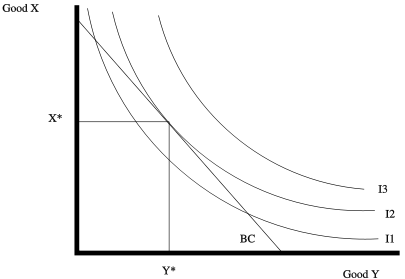
\includegraphics{images/constraint.png}
\caption{A typical Utility Function with a Budget Constraint}
\end{figure}

\textbf{Types of Constraints}: For a function \(f(x_1, \dots, x_n)\), there are two types of constraints that can be imposed:

\begin{enumerate}
\item \textbf{Equality constraints:} constraints of the form $c(x_1,\dots, x_n) = r$.
Budget constraints are the classic example of equality constraints in social science.
\item \textbf{Inequality constraints:} constraints of the form $c(x_1, \dots, x_n) \leq r$.  These might arise from non-negativity constraints or other threshold effects.
\end{enumerate}

In any constrained optimization problem, the constrained maximum will always be less than or equal to the unconstrained maximum. If the constrained maximum is less than the unconstrained maximum, then the constraint is binding. Essentially, this means that you can treat your constraint as an equality constraint rather than an inequality constraint.

For example, the budget constraint binds when you spend your entire budget. This generally happens because we believe that utility is strictly increasing in consumption, i.e.~you always want more so you spend everything you have.

Any number of constraints can be placed on an optimization problem. When working with multiple constraints, always make sure that the set of constraints are not pathological; it must be possible for all of the constraints to be satisfied simultaneously.

\textbf{Set-up for Constrained Optimization:}
\[\max_{x_1,x_2} f(x_1,x_2) \text{ s.t. } c(x_1,x_2)\]
\[\min_{x_1,x_2} f(x_1,x_2) \text{ s.t. } c(x_1,x_2)\]
This tells us to maximize/minimize our function, \(f(x_1,x_2)\), with respect to the choice variables, \(x_1,x_2\), subject to the constraint.

Example:
\[\max_{x_1,x_2} f(x_1, x_2) = -(x_1^2 + 2x_2^2) \text{ s.t. }x_1 + x_2 = 4\]
It is easy to see that the \textit{unconstrained} maximum occurs at \((x_1, x_2) = (0,0)\), but that does not satisfy the constraint. How should we proceed?

\hypertarget{equality-constraints}{%
\subsection*{Equality Constraints}\label{equality-constraints}}
\addcontentsline{toc}{subsection}{Equality Constraints}

Equality constraints are the easiest to deal with because we know that the maximum or minimum has to lie on the (intersection of the) constraint(s).

The trick is to change the problem from a constrained optimization problem in \(n\) variables to an unconstrained optimization problem in \(n + k\) variables, adding \emph{one} variable for \emph{each} equality constraint. We do this using a lagrangian multiplier.

\textbf{Lagrangian function}: The Lagrangian function allows us to combine the function we want to optimize and the constraint function into a single function. Once we have this single function, we can proceed as if this were an \emph{unconstrained} optimization problem.

For each constraint, we must include a \textbf{Lagrange multiplier} (\(\lambda_i\)) as an additional variable in the analysis. These terms are the link between the constraint and the Lagrangian function.

Given a \emph{two dimensional} set-up:
\[\max_{x_1,x_2}/\min_{x_1,x_2} f(x_1,x_2) \text{ s.t. } c(x_1,x_2) = a\]

We define the Lagrangian function \(L(x_1,x_2,\lambda_1)\) as follows:
\[L(x_1,x_2,\lambda_1) = f(x_1,x_2) - \lambda_1 (c(x_1,x_2) - a)\]

More generally, in \emph{n dimensions}:
\[ L(x_1, \dots, x_n, \lambda_1, \dots, \lambda_k) = f(x_1, \dots, x_n) - \sum_{i=1}^k\lambda_i(c_i(x_1,\dots, x_n) - r_i)\]

\textbf{Getting the sign right:} Note that above we subtract the lagrangian term \emph{and} we subtract the constraint constant from the constraint function. Occasionally, you may see the following alternative form of the Lagrangian, which is \emph{equivalent}:
\[ L(x_1, \dots, x_n, \lambda_1, \dots, \lambda_k) = f(x_1, \dots, x_n) + \sum_{i=1}^k\lambda_i(r_i - c_i(x_1,\dots, x_n))\]
Here we add the lagrangian term \emph{and} we subtract the constraining function from the constraint constant.

\textbf{Using the Lagrangian to Find the Critical Points}: To find the critical points, we take the partial derivatives of lagrangian function, \(L(x_1, \dots, x_n, \lambda_1, \dots, \lambda_k)\), with respect to each of its variables (all choice variables \(\mathbf{x}\) \emph{and} all lagrangian multipliers \(\mathbf{\lambda}\)). At a critical point, each of these partial derivatives must be equal to zero, so we obtain a system of \(n + k\) equations in \(n + k\) unknowns:

\begin{align*}
\frac{\partial L}{\partial x_1} &= \frac{\partial f}{\partial x_1} - \sum_{i = 1}^k\lambda_i\frac{\partial c_i}{\partial x_1} = 0\\
 \vdots &= \vdots \nonumber \\ 
\frac{\partial L}{\partial x_n}  &= \frac{\partial f}{\partial x_n} - \sum_{i = 1}^k\lambda_i\frac{\partial c_i}{\partial x_n} = 0\\
\frac{\partial L}{\partial \lambda_1} &= c_1(x_i, \dots, x_n) - r_1 =  0\\
 \vdots &= \vdots \nonumber \\
\frac{\partial L}{\partial \lambda_k} &= c_k(x_i, \dots, x_n) - r_k = 0
\end{align*}

We can then solve this system of equations, because there are \(n+k\) equations and \(n+k\) unknowns, to calculate the critical point \((x_1^*,\dots,x_n^*,\lambda_1^*,\dots,\lambda_k^*)\).

\textbf{Second-order Conditions and Unconstrained Optimization:} There may be more than one critical point, i.e.~we need to verify that the critical point we find is a maximum/minimum. Similar to unconstrained optimization, we can do this by checking the second-order conditions.

\BeginKnitrBlock{example}[Constrained optimization with two goods and a budget constraint]
\protect\hypertarget{exm:unnamed-chunk-60}{}{\label{exm:unnamed-chunk-60} \iffalse (Constrained optimization with two goods and a budget constraint) \fi{} }
Find the constrained optimization of
\[\max_{x_1,x_2} f(x) = -(x_1^2 + 2x_2^2) \text{ s.t. } x_1 + x_2 = 4\]
\EndKnitrBlock{example}

\BeginKnitrBlock{solution}
\iffalse{} {Solution. } \fi{}
1. Begin by writing the Lagrangian:
\[L(x_1, x_2, \lambda) =  -(x_1^2 + 2x_2^2) - \lambda(x_1 + x_2 - 4)\]
2. Take the partial derivatives and set equal to zero:

\begin{align*}
\frac{\partial L}{\partial x_1} = -2x_1 - \lambda \quad \quad \quad &= 0\\
\frac{\partial L}{\partial x_2}  = -4x_2 - \lambda \quad \quad \quad &= 0\\
\frac{\partial L}{\partial \lambda} = -(x_1 + x_2 - 4) \quad & = & 0\\
\end{align*}

\begin{enumerate}
\def\labelenumi{\arabic{enumi}.}
\setcounter{enumi}{2}
\item
  Solve the system of equations: Using the first two partials, we see that \(\lambda = -2x_1\) and \(\lambda = -4x_2\)
  Set these equal to see that \(x_1 = 2x_2\).
  Using the third partial and the above equality, \(4 = 2x_2 + x_2\) from which we get \[x_2^* = 4/3, x_1^* = 8/3, \lambda = -16/3\]
\item
  Therefore, the only critical point is \(x_1^* = \frac{8}{3}\) and \(x_2^* = \frac{4}{3}\)
\item
  This gives \(f(\frac{8}{3}, \frac{4}{3}) = -\frac{96}{9}\), which is less than the unconstrained optimum \(f(0,0) = 0\)
\end{enumerate}
\EndKnitrBlock{solution}

Notice that when we take the partial derivative of L with respect to the Lagrangian multiplier and set it equal to 0, we return exactly our constraint! This is why signs matter.

\hypertarget{inequality-constraints}{%
\section{Inequality Constraints}\label{inequality-constraints}}

Inequality constraints define the boundary of a region over which we seek to optimize the function. This makes inequality constraints more challenging because we do not know if the maximum/minimum lies along one of the constraints (the constraint binds) or in the interior of the region.

We must introduce more variables in order to turn the problem into an unconstrained optimization.

\textbf{Slack:} For each inequality constraint \(c_i(x_1, \dots, x_n) \leq a_i\), we define a slack variable \(s_i^2\) for which the expression \(c_i(x_1, \dots, x_n) \leq a_i - s_i^2\) would hold with equality. These slack variables capture how close the constraint comes to binding. We use \(s^2\) rather than \(s\) to ensure that the slack is positive.

Slack is just a way to transform our constraints.

Given a two-dimensional set-up and these edited constraints:
\[\max_{x_1,x_2}/\min_{x_1,x_2} f(x_1,x_2) \text{ s.t. } c(x_1,x_2) \le a_1\]

Adding in Slack:
\[\max_{x_1,x_2}/\min_{x_1,x_2} f(x_1,x_2) \text{ s.t. } c(x_1,x_2) \le a_1 - s_1^2\]

We define the Lagrangian function \(L(x_1,x_2,\lambda_1,s_1)\) as follows:
\[L(x_1,x_2,\lambda_1,s_1) = f(x_1,x_2) - \lambda_1 ( c(x_1,x_2) + s_1^2 - a_1)\]

More generally, in n dimensions:
\[ L(x_1, \dots, x_n, \lambda_1, \dots, \lambda_k, s_1, \dots, s_k) = f(x_1, \dots, x_n) - \sum_{i = 1}^k \lambda_i(c_i(x_1,\dots, x_n) + s_i^2 - a_i)\]

\textbf{Finding the Critical Points}: To find the critical points, we take the partial derivatives of the lagrangian function, \(L(x_1,\dots,x_n,\lambda_1,\dots,\lambda_k,s_1,\dots,s_k)\), with respect to each of its variables (all choice variables \(x\), all lagrangian multipliers \(\lambda\), and all slack variables \(s\)). At a critical point, \emph{each} of these partial derivatives must be equal to zero, so we obtain a system of \(n + 2k\) equations in \(n + 2k\) unknowns:

\begin{align*}
\frac{\partial L}{\partial x_1} &= \frac{\partial f}{\partial x_1} - \sum_{i = 1}^k\lambda_i\frac{\partial c_i}{\partial x_1} = 0\\
 \vdots & =  \vdots  \\
\frac{\partial L}{\partial x_n}  &= \frac{\partial f}{\partial x_n} - \sum_{i = 1}^k\lambda_i\frac{\partial c_i}{\partial x_n} = 0\\
\frac{\partial L}{\partial \lambda_1} &= c_1(x_i, \dots, x_n) + s_1^2 - b_1 = 0\\
 \vdots & = \vdots \\
\frac{\partial L}{\partial \lambda_k} &= c_k(x_i, \dots, x_n) + s_k^2 - b_k = 0\\
\frac{\partial L}{\partial s_1} &= 2s_1\lambda_1 = 0\\
 \vdots =\vdots \\
\frac{\partial L}{\partial s_k} &= 2s_k\lambda_k = 0
\end{align*}

\textbf{Complementary slackness conditions}: The last set of first order conditions of the form \(2s_i\lambda_i = 0\) (the partials taken with respect to the slack variables) are known as complementary slackness conditions. These conditions can be satisfied one of three ways:

\begin{enumerate}
\def\labelenumi{\arabic{enumi}.}
\tightlist
\item
  \(\lambda_i = 0\) and \(s_i \neq 0\): This implies that the slack is positive and thus \emph{the constraint does not bind}.
\item
  \(\lambda_i \neq 0\) and \(s_i = 0\): This implies that there is no slack in the constraint and \emph{the constraint does bind}.
\item
  \(\lambda_i = 0\) and \(s_i = 0\): In this case, there is no slack but the \emph{constraint binds trivially}, without changing the optimum.
\end{enumerate}

Example: Find the critical points for the following constrained optimization:
\[\max_{x_1,x_2} f(x) = -(x_1^2 + 2x_2^2) \text{ s.t. } x_1 + x_2 \le 4\]

\begin{enumerate}
\def\labelenumi{\arabic{enumi}.}
\item
  Rewrite with the slack variables:
  \[\max_{x_1,x_2} f(x) = -(x_1^2 + 2x_2^2) \text{ s.t. } x_1 + x_2 \le 4 - s_1^2\]
\item
  Write the Lagrangian:
  \[L(x_1,x_2,\lambda_1,s_1) = -(x_1^2 + 2x_2^2) - \lambda_1 (x_1 + x_2 + s_1^2 - 4)\]
\item
  Take the partial derivatives and set equal to 0:
\end{enumerate}

\begin{align*}
\frac{\partial L}{\partial x_1} = -2x_1 - \lambda_1  &= 0\\
\frac{\partial L}{\partial x_2}  = -4x_2 - \lambda_1 &=  0\\
\frac{\partial L}{\partial \lambda_1} = -(x_1 + x_2 + s_1^2 - 4)&= 0\\
\frac{\partial L}{\partial s_1} = -2s_1\lambda_1 &= 0\\
\end{align*}

\begin{enumerate}
\def\labelenumi{\arabic{enumi}.}
\setcounter{enumi}{3}
\tightlist
\item
  Consider all ways that the complementary slackness conditions are solved:

  \begin{center}
  \begin{tabular}{|l|cccc|c|}
  \hline
  Hypothesis & $s_1$ & $\lambda_1$ & $x_1$ & $x_2$ & $f(x_1, x_2)$\\
  \hline
  $s_1 = 0$ $\lambda_1 = 0$ & \multicolumn{4}{l|}{No solution} & \\
  $s_1 \neq 0$ $\lambda_1 = 0$ & 2 & 0 & 0 & 0  & 0\\
  $s_1 = 0$ $\lambda_1 \neq 0$ & 0 & $\frac{-16}{3}$ & $\frac{8}{3}$ & $\frac{4}{3}$ & $-\frac{32}{3}$\\
  $s_1 \neq 0$ $\lambda_1 \neq 0$ & \multicolumn{4}{l|}{No solution} &\\
  \hline
  \end{tabular}
  \end{center}
\end{enumerate}

This shows that there are two critical points: \((0,0)\) and \((\frac{8}{3},\frac{4}{3})\).

\begin{enumerate}
\def\labelenumi{\arabic{enumi}.}
\setcounter{enumi}{4}
\tightlist
\item
  Find maximum:
  Looking at the values of \(f(x_1,x_2)\) at the critical points, we see that \(f(x_1,x_2)\) is maximized at \(x_1^* = 0\) and \(x_2^*=0\).
\end{enumerate}

\BeginKnitrBlock{exercise}
\protect\hypertarget{exr:unnamed-chunk-62}{}{\label{exr:unnamed-chunk-62} }Example: Find the critical points for the following constrained optimization:
\[\max_{x_1,x_2} f(x) = -(x_1^2 + 2x_2^2) \text{ s.t. } 
\begin{array}{l}
x_1 + x_2 \le 4\\
x_1 \ge 0\\
x_2 \ge 0
\end{array}\]
\EndKnitrBlock{exercise}

\begin{enumerate}
\def\labelenumi{\arabic{enumi}.}
\item
  Rewrite with the slack variables:
  \[\phantom{max_{x_1,x_2} f(x) = -(x_1^2 + 2x_2^2) \text{ s.t. } 
  \begin{array}{l}
  x_1 + x_2 \le 4 - s_1^2\\
  -x_1 \le 0 - s_2^2\\
  -x_2 \le 0 - s_3^2
  \end{array}}\]
\item
  Write the Lagrangian:
  \[\phantom{L(x_1, x_2, \lambda_1, \lambda_2, \lambda_3, s_1, s_2, s_3) =  -(x_1^2 + 2x_2^2) - \lambda_1(x_1 + x_2 + s_1^2  - 4) - \lambda_2(-x_1 + s_2^2) - \lambda_3(-x_2 + s_3^2)}\]
\item
  Take the partial derivatives and set equal to zero:
\end{enumerate}

\phantom{
$\frac{\partial L}{\partial x_1} = -2x_1 - \lambda_1 + \lambda_2  =  0$\\
$\frac{\partial L}{\partial x_2}  = -4x_2 - \lambda_1 + \lambda_3  =   0$\\
$\frac{\partial L}{\partial \lambda_1} = -(x_1 + x_2 + s_1^2 - 4) =  0$\\
$\frac{\partial L}{\partial \lambda_2} = -(-x_1 + s_2^2)  =  0$\\
$\frac{\partial L}{\partial \lambda_3} = -(-x_2 + s_3^2)  =  0$\\
$\frac{\partial L}{\partial s_1} = 2s_1\lambda_1  =  0$\\
$\frac{\partial L}{\partial s_2} = 2s_2\lambda_2  =  0$\\
$\frac{\partial L}{\partial s_3} = 2s_3\lambda_3  =  0$}

\begin{enumerate}
\def\labelenumi{\arabic{enumi}.}
\setcounter{enumi}{3}
\tightlist
\item
  Consider all ways that the complementary slackness conditions are solved:

  \begin{center}
  \begin{tabular}{|l|cccccccc|c|}
  \hline
  Hypothesis & $s_1$ & $s_2$ & $s_3$ & $\lambda_1$ & $\lambda_2$ & $\lambda_3$ & $x_1$ & $x_2$ & $f(x_1, x_2)$\\
  \hline
  $s_1 = s_2 = s_3 = 0$ & \multicolumn{8}{l|}{\phantom{No solution}} & \\
  $s_1 \neq 0, s_2 = s_3 = 0$ & \phantom{2} & \phantom{0} & \phantom{0} & \phantom{0} & \phantom{0} & \phantom{0} & \phantom{0} & \phantom{0} & \phantom{0}\\
  $s_2 \neq 0, s_1 = s_3 = 0$ & \phantom{0} & \phantom{2} & \phantom{0} & \phantom{-8} & \phantom{0} & \phantom{-8} & \phantom{4} & \phantom{0} & \phantom{-16}\\
  $s_3 \neq 0, s_1 = s_2 = 0$ & \phantom{0} & \phantom{0} & \phantom{2} & \phantom{-16} & \phantom{-16} & \phantom{0} & \phantom{0} & \phantom{4} & \phantom{-32}\\
  $s_1 \neq 0, s_2 \neq 0, s_3 = 0$ &\multicolumn{8}{l|}{\phantom{No solution}} & \\
  $s_1 \neq 0, s_3 \neq 0, s_2 = 0$ &\multicolumn{8}{l|}{\phantom{No solution}} & \\
  $s_2 \neq 0, s_3 \neq 0, s_1 = 0$ &\phantom{0} & \phantom{$\sqrt{\frac{8}{3}}$} & \phantom{$\sqrt{\frac{4}{3}}$} & \phantom{$-\frac{16}{3}$} & \phantom{0} & \phantom{0} & \phantom{$\frac{8}{3}$}& \phantom{$\frac{4}{3}$} & \phantom{$-\frac{32}{3}$}\\
  $s_1 \neq 0, s_2 \neq 0, s_3 \neq 0$ &\multicolumn{8}{l|}{\phantom{No solution}}& \\
  \hline
  \end{tabular}
  \end{center}
\end{enumerate}

\phantom{This shows that there are four critical points: $(0,0)$, $(4,0)$, $(0,4)$, and $(\frac{8}{3},\frac{4}{3})$}

\begin{enumerate}
\def\labelenumi{\arabic{enumi}.}
\setcounter{enumi}{4}
\tightlist
\item
  Find maximum: \phantom{Looking at the values of $f(x_1,x_2)$ at the critical points, we see that the constrained maximum is located at $(x_1, x_2) = (0,0)$, which is the same as the unconstrained max.  The constrained minimum is located at $(x_1, x_2) = (0,4)$, while there is no unconstrained minimum for this problem.}
\end{enumerate}

\hypertarget{kuhn-tucker-conditions}{%
\section{Kuhn-Tucker Conditions}\label{kuhn-tucker-conditions}}

As you can see, this can be a pain. When dealing explicitly with \emph{non-negativity constraints}, this process is simplified by using the Kuhn-Tucker method.

Because the problem of maximizing a function subject to inequality and non-negativity constraints arises frequently in economics, the \textbf{Kuhn-Tucker conditions} provides a method that often makes it easier to both calculate the critical points and identify points that are (local) maxima.

Given a \emph{two-dimensional set-up}:
\[\max_{x_1,x_2}/\min_{x_1,x_2} f(x_1,x_2) \text{ s.t. }
\begin{array}{l}
c(x_1,x_2) \le a_1\\
x_1 \ge 0 \\
gx_2 \ge 0
\end{array}\]

We define the Lagrangian function \(L(x_1,x_2,\lambda_1)\) the same as if we did not have the non-negativity constraints:
\[L(x_1,x_2,\lambda_2) = f(x_1,x_2) - \lambda_1(c(x_1,x_2) - a_1)\]

More generally, in n dimensions:
\[ L(x_1, \dots, x_n, \lambda_1, \dots, \lambda_k) = f(x_1, \dots, x_n) - \sum_{i=1}^k\lambda_i(c_i(x_1,\dots, x_n) - a_i)\]

\textbf{Kuhn-Tucker and Complementary Slackness Conditions}: To find the critical points, we first calculate the Kuhn-Tucker conditions by taking the partial derivatives of the lagrangian function, \(L(x_1,\dots,x_n,\lambda_1,\dots,\lambda_k)\), with respect to each of its variables (all choice variable s\(x\) and all lagrangian multipliers \(\lambda\)) and we calculate the \emph{complementary slackness conditions} by multiplying each partial derivative by its respective variable \emph{and} include non-negativity conditions for all variables (choice variables \(x\) and lagrangian multipliers \(\lambda\)).

\textbf{Kuhn-Tucker Conditions}

\begin{align*}
\frac{\partial L}{\partial x_1} \leq 0, & \dots, \frac{\partial L}{\partial x_n} \leq 0\\
\frac{\partial L}{\partial \lambda_1} \geq 0, & \dots, \frac{\partial L}{\partial \lambda_m} \geq 0
\end{align*}

\textbf{Complementary Slackness Conditions}

\begin{align*}
x_1\frac{\partial L}{\partial x_1} = 0, & \dots, x_n\frac{\partial L}{\partial x_n} = 0\\
\lambda_1\frac{\partial L}{\partial \lambda_1} = 0, & \dots, \lambda_m \frac{\partial L}{\partial \lambda_m} = 0
\end{align*}

\textbf{Non-negativity Conditions}
\begin{eqnarray*}
x_1 \geq 0 & \dots & x_n \geq 0\\
\lambda_1 \geq 0 & \dots & \lambda_m \geq 0
\end{eqnarray*}

Note that some of these conditions are set equal to 0, while others are set as inequalities!

Note also that to minimize the function \(f(x_1, \dots, x_n)\), the simplest thing to do is maximize the function \(-f(x_1, \dots, x_n)\); all of the conditions remain the same after reformulating as a maximization problem.

There are additional assumptions (notably, f(x) is quasi-concave and the constraints are convex) that are sufficient to ensure that a point satisfying the Kuhn-Tucker conditions is a global max; if these assumptions do not hold, you may have to check more than one point.

\textbf{Finding the Critical Points with Kuhn-Tucker Conditions}: Given the above conditions, to find the critical points we solve the above system of equations. To do so, we must check \textit{all} border and interior solutions to see if they satisfy the above conditions.

In a two-dimensional set-up, this means we must check the following cases:

\begin{enumerate}
\def\labelenumi{\arabic{enumi}.}
\tightlist
\item
  \(x_1 = 0, x_2 = 0\) Border Solution
\item
  \(x_1 = 0, x_2 \neq 0\) Border Solution
\item
  \(x_1 \neq 0, x_2 = 0\) Border Solution
\item
  \(x_1 \neq 0, x_2 \neq 0\) Interior Solution
\end{enumerate}

\BeginKnitrBlock{example}[Kuhn-Tucker with two variables]
\protect\hypertarget{exm:unnamed-chunk-63}{}{\label{exm:unnamed-chunk-63} \iffalse (Kuhn-Tucker with two variables) \fi{} }Solve the following optimization problem with inequality constraints
\[\max_{x_1,x_2} f(x) = -(x_1^2 + 2x_2^2)\]

\begin{align*}
\text{ s.t. } 
\begin{cases}
&x_1 + x_2 *\le 4\\
&x_1 *\ge 0\\
&x_2 *\ge 0
\end{cases}
\end{align*}
\EndKnitrBlock{example}

\begin{enumerate}
\def\labelenumi{\arabic{enumi}.}
\item
  Write the Lagrangian:
  \[L(x_1, x_2, \lambda) =  -(x_1^2 + 2x_2^2) - \lambda(x_1 + x_2 - 4)\]
\item
  Find the First Order Conditions:
\end{enumerate}

Kuhn-Tucker Conditions
\begin{align*}
\frac{\partial L}{\partial x_1} = -2x_1 - \lambda  &\leq 0\\
\frac{\partial L}{\partial x_2}  = -4x_2 - \lambda & \leq  0\\
\frac{\partial L}{\partial \lambda} = -(x_1 + x_2 - 4)& \geq 0
\end{align*}

Complementary Slackness Conditions
\begin{align*}
x_1\frac{\partial L}{\partial x_2} = x_1(-2x_1 - \lambda)  &= 0\\
x_2\frac{\partial L}{\partial x_2} = x_2(-4x_2 - \lambda)  &= 0\\
\lambda\frac{\partial L}{\partial \lambda} = -\lambda(x_1 + x_2 - 4)&= 0
\end{align*}

Non-negativity Conditions
\begin{align*}
x_1 & \geq  0\\
x_2 & \geq 0\\
\lambda & \geq 0
\end{align*}

\begin{enumerate}
\def\labelenumi{\arabic{enumi}.}
\setcounter{enumi}{2}
\tightlist
\item
  Consider all border and interior cases:

  \begin{center}
  \begin{tabular}{|l|ccc|c|}
  \hline
  Hypothesis  & $\lambda$& $x_1$ & $x_2$ & $f(x_1, x_2)$\\
  \hline
  $x_1 = 0, x_2 = 0$  &0 & 0 & 0 & 0\\
  $x_1 = 0, x_2 \neq 0$  &-16 & 0 & 4 & -32\\
  $x_1 \neq 0, x_2 = 0$  &-8 & 4 & 0 & -16\\
  $x_1 \neq 0, x_2 \neq 0$ & $-\frac{16}{3}$ & $\frac{8}{3}$ & $\frac{4}{3}$ & $-\frac{32}{3}$\\
  \hline
  \end{tabular}
  \end{center}
\item
  Find Maximum:
  Three of the critical points violate the requirement that \(\lambda \geq 0\), so the point \((0,0,0)\) is the maximum.
\end{enumerate}

\BeginKnitrBlock{exercise}[Kuhn-Tucker with logs]
\protect\hypertarget{exr:unnamed-chunk-64}{}{\label{exr:unnamed-chunk-64} \iffalse (Kuhn-Tucker with logs) \fi{} }Solve the constrained optimization problem,

\[\max_{x_1,x_2} f(x) = \frac{1}{3}\log (x_1 + 1) + \frac{2}{3}\log (x_2 + 1) \text{ s.t. }  
\begin{array}{l}
x_1 + 2x_2 \leq 4\\
     x_1 \geq 0\\
    x_2 \geq 0
\end{array}\]
\EndKnitrBlock{exercise}

\begin{enumerate}
\item Write the Lagrangian:
$$\phantom{L(x_1, x_2, \lambda) =  \frac{1}{3}\log(x_1+1) + \frac{2}{3}\log(x_2+1) - \lambda(x_1 + 2x_2 - 4)}$$

\item Find the First Order Conditions:\\
Kuhn-Tucker Conditions\\
\phantom{$\frac{\partial L}{\partial x_1} = \frac{1}{3(x_1+1)} - \lambda   \leq  0$\\
$\frac{\partial L}{\partial x_2}  = \frac{2}{3(x_2+1)} - \lambda  \leq   0$\\
$\frac{\partial L}{\partial \lambda} = -(x_1 + 2x_2 - 4) \geq  0$}\\
\item[]
\item[]
\item[]
\item[]
\item[]
\item[]
\item[]
\item[]
 
Complementary Slackness Conditions\\
\phantom{$x_1\frac{\partial L}{\partial x_2} = x_1(\frac{1}{3(x_1+1)} - \lambda)  =  0$\\
$x_2\frac{\partial L}{\partial x_2} = x_2(\frac{2}{3(x_2+1)} - \lambda)   =  0$\\
$\lambda\frac{\partial L}{\partial \lambda} = -\lambda(x_1 + 2x_2 - 4) =  0$}\\
\item[]
\item[]
\item[]
\item[]
\item[]
\item[]
\item[]
\item[]
\item[]

Non-negativity Conditions\\
\phantom{$x_1  \geq  0$\\
$x_2  \geq  0$\\
$\lambda  \geq  $0}\\
\item[]
\item[]
\item[]

\item Consider all border and interior cases:
\begin{center}
\begin{tabular}{|l|ccc|c|}
\hline
Hypothesis  & $\lambda$& $x_1$ & $x_2$ & $f(x_1, x_2)$\\
\hline
$x_1 = 0, x_2 = 0$  &\multicolumn{3}{l|}{\phantom{No Solution}}& \\
$x_1 = 0, x_2 \neq 0$  &\multicolumn{3}{l|}{\phantom{No Solution}}& \\
$x_1 \neq 0, x_2 = 0$  & \multicolumn{3}{l|}{\phantom{No Solution}}& \\
$x_1 \neq 0, x_2 \neq 0$ &  & \phantom{$\frac{4}{3}$} & \phantom{$\frac{4}{3}$} & \phantom{$\log\frac{7}{3}$}\\
\hline
\end{tabular}
\end{center}

\item[]
\item[]
\item[]
\item[]

\item  Find Maximum:\\
\phantom{Three of the critical points violate the constraints, so the point $(\frac{4}{3},\frac{4}{3})$ is the maximum.}\\
\end{enumerate}

\hypertarget{applications-of-quadratic-forms}{%
\section{Applications of Quadratic Forms}\label{applications-of-quadratic-forms}}

\textbf{Curvature and The Taylor Polynomial as a Quadratic Form}:
The Hessian is used in a Taylor polynomial approximation to \(f(\mathbf{x})\) and provides information about the curvature of \(f({\bf x})\) at \(\mathbf{x}\) --- e.g., which tells us whether a critical point \(\mathbf{x}^*\) is a min, max, or saddle point.

\begin{enumerate}
\def\labelenumi{\arabic{enumi}.}
\tightlist
\item
  The second order Taylor polynomial about the critical point
  \({\bf x}^*\) is
  \[f({\bf x}^*+\bf h)=f({\bf x}^*)+\nabla f({\bf x}^*) \bf h +\frac{1}{2} \bf h^\top
  {\bf H(x^*)} \bf h + R(\bf h)\]
\item
  Since we're looking at a critical point, \(\nabla f({\bf x}^*)=0\);
  and for small \(\bf h\), \(R(\bf h)\) is negligible. Rearranging, we get
  \[f({\bf x}^*+\bf h)-f({\bf x}^*)\approx \frac{1}{2} \bf h^\top {\bf H(x^*)}
  \bf h \]
\item
  The Righthand side here is a quadratic form and we can determine the definiteness of \(\bf H(x^*)\).
\end{enumerate}

\hypertarget{probability-theory}{%
\chapter{Probability Theory}\label{probability-theory}}

Probability and Inferences are mirror images of each other, and both are integral to social science. Probability quantifies uncertainty, which is important because many things in the social world are at first uncertain. Inference is then the study of how to learn about facts you don't observe from facts you do observe.

\hypertarget{counting-rules}{%
\section{Counting rules}\label{counting-rules}}

\textbf{Fundamental Theorem of Counting}: If an object has \(j\) different characteristics that are independent of each other, and each characteristic \(i\) has \(n_i\) ways of being expressed, then there are \(\prod_{i = 1}^j n_i\) possible unique objects.

Example: Cards can be either red or black and can take on any of 13 values.

\(j =\)

\(n_{\text{color}} =\)

\(n_{\text{number}} =\)

Number of Outcomes \(=\)

We often need to count the number of ways to choose a subset from some set of possibilities. The number of outcomes depends on two characteristics of the process: does the order matter and is replacement allowed?

\textbf{Sampling Table}: If there are \(n\) objects which are numbered 1 to \(n\) and we select \(k < n\) of them, how many different outcomes are possible?

If the order in which a given object is selected matters, selecting 4 numbered objects in the following order (1, 3, 7, 2) and selecting the same four objects but in a different order such as (7, 2, 1, 3) will be counted as different outcomes.

If replacement is allowed, there are always the same \(n\) objects to select from. However, if replacement is not allowed, there is always one less option than the previous round when making a selection. For example, if replacement is not allowed and I am selecting 3 elements from the following set \{1, 2, 3, 4, 5, 6\}, I will have 6 options at first, 5 options as I make my second selection, and 4 options as I make my third.

So in counting how many different outcomes are possible, if \textbf{\emph{order matters}} AND we are sampling \textbf{\emph{with replacement}}, the number of different outcomes is \(n^k\).

If \textbf{\emph{order matters}} AND we are sampling \textbf{\emph{without replacement}}, the number of different outcomes is \(n(n-1)(n-2)...(n-k+1)=\frac{n!}{(n-k)!}\).

If \textbf{\emph{order doesn't matter}} AND we are sampling \textbf{\emph{without replacement}}, the number of different outcomes is \(\binom{n}{k} = \frac{n!}{(n-k)!k!}\).

Expression \(\binom{n}{k}\) is read as ``n choose k'' and denotes \(\frac{n!}{(n-k)!k!}\). Also, note that \(0! = 1\).

\BeginKnitrBlock{example}[Counting]
\protect\hypertarget{exm:counting}{}{\label{exm:counting} \iffalse (Counting) \fi{} }
There are five balls numbered from 1 through 5 in a jar. Three balls are chosen. How many possible choices are there?

\begin{enumerate}
\def\labelenumi{\arabic{enumi}.}
\item
  Ordered, with replacement \(=\)
\item
  Ordered, without replacement \(=\)
\item
  Unordered, without replacement \(=\)
\end{enumerate}
\EndKnitrBlock{example}

\BeginKnitrBlock{exercise}[Counting]
\protect\hypertarget{exr:counting1}{}{\label{exr:counting1} \iffalse (Counting) \fi{} }
Four cards are selected from a deck of 52 cards. Once a card has been drawn, it is not reshuffled back into the deck. Moreover, we care only about the complete hand that we get (i.e.~we care about the set of selected cards, not the sequence in which it was drawn). How many possible outcomes are there?
\EndKnitrBlock{exercise}

\hypertarget{setoper}{%
\section{Sets}\label{setoper}}

\textbf{Set} : A set is any well defined collection of elements. If \(x\) is an element of \(S\), \(x \in S\).

\textbf{Sample Space (S)}: A set or collection of all possible outcomes from some process. Outcomes in the set can be discrete elements (countable) or points along a continuous interval (uncountable).

Examples:

\begin{enumerate}
\def\labelenumi{\arabic{enumi}.}
\tightlist
\item
  Discrete: the numbers on a die, whether a vote cast is republican or democrat.
\item
  Continuous: GNP, arms spending, age.
\end{enumerate}

\textbf{Event}: Any collection of possible outcomes of an experiment. Any subset of the full set of possibilities, including the full set itself. Event A \(\subset\) S.

\textbf{Empty Set}: a set with no elements. \(S = \{\}\). It is denoted by the symbol \(\emptyset\).

Set operations:

\begin{enumerate}
\def\labelenumi{\arabic{enumi}.}
\tightlist
\item
  \textbf{Union}: The union of two sets \(A\) and \(B\), \(A \cup B\), is the set containing all of the elements in \(A\) or \(B\). \[A_1 \cup A_2  \cup \cdots \cup A_n = \bigcup_{i=1}^n A_i\]
\item
  \textbf{Intersection}: The intersection of sets \(A\) and \(B\), \(A \cap B\), is the set containing all of the elements in both \(A\) and \(B\). \[A_1 \cap A_2  \cap \cdots \cap A_n = \bigcap_{i=1}^n A_i\]
\item
  \textbf{Complement}: If set \(A\) is a subset of \(S\), then the complement of \(A\), denoted \(A^C\), is the set containing all of the elements in \(S\) that are not in \(A\).
\end{enumerate}

Properties of set operations:

\begin{itemize}
\tightlist
\item
  \textbf{Commutative}: \(A \cup B = B \cup A\); \(A \cap B = B \cap A\)
\item
  \textbf{Associative}: \(A \cup (B \cup C) = (A \cup B) \cup C\); \(A \cap (B \cap C) = (A \cap B) \cap C\)
\item
  \textbf{Distributive}: \(A \cap (B \cup C) = (A \cap B) \cup (A \cap C)\); \(A \cup (B \cap C) = (A \cup B) \cap (A \cup C)\)
\item
  \textbf{de Morgan's laws}: \((A \cup B)^C = A^C \cap B^C\); \((A \cap B)^C = A^C \cup B^C\)
\item
  \textbf{Disjointness}: Sets are disjoint when they do not intersect, such that \(A \cap B = \emptyset\). A collection of sets is pairwise disjoint (\textbf{mutually exclusive}) if, for all \(i \neq j\), \(A_i \cap A_j = \emptyset\). A collection of sets form a partition of set \(S\) if they are pairwise disjoint and they cover set \(S\), such that \(\bigcup_{i = 1}^k A_i = S\).
\end{itemize}

\BeginKnitrBlock{example}[Sets]
\protect\hypertarget{exm:sets}{}{\label{exm:sets} \iffalse (Sets) \fi{} }
Let set \(A\) be \{1, 2, 3, 4\}, \(B\) be \{3, 4, 5, 6\}, and \(C\) be \{5, 6, 7, 8\}. Sets \(A\), \(B\), and \(C\) are all subsets of the sample space \(S\) which is \{1, 2, 3, 4, 5, 6, 7, 8, 9, 10\}

Write out the following sets:

\begin{enumerate}
\def\labelenumi{\arabic{enumi}.}
\tightlist
\item
  \(A \cup B\)
\item
  \(C \cap B\)
\item
  \(B^c\)
\item
  \(A \cap (B \cup C)\)
\end{enumerate}
\EndKnitrBlock{example}

\BeginKnitrBlock{exercise}[Sets]
\protect\hypertarget{exr:sets1}{}{\label{exr:sets1} \iffalse (Sets) \fi{} }

Suppose you had a pair of four-sided dice. You sum the results from a single toss.

What is the set of possible outcomes (i.e.~the sample space)?

Consider subsets A \{2, 8\} and B \{2,3,7\} of the sample space you found. What is

\begin{enumerate}
\def\labelenumi{\arabic{enumi}.}
\tightlist
\item
  \(A^c\)
\item
  \((A \cup B)^c\)
\end{enumerate}
\EndKnitrBlock{exercise}

\hypertarget{probdef}{%
\section{Probability}\label{probdef}}

\begin{figure}
\centering
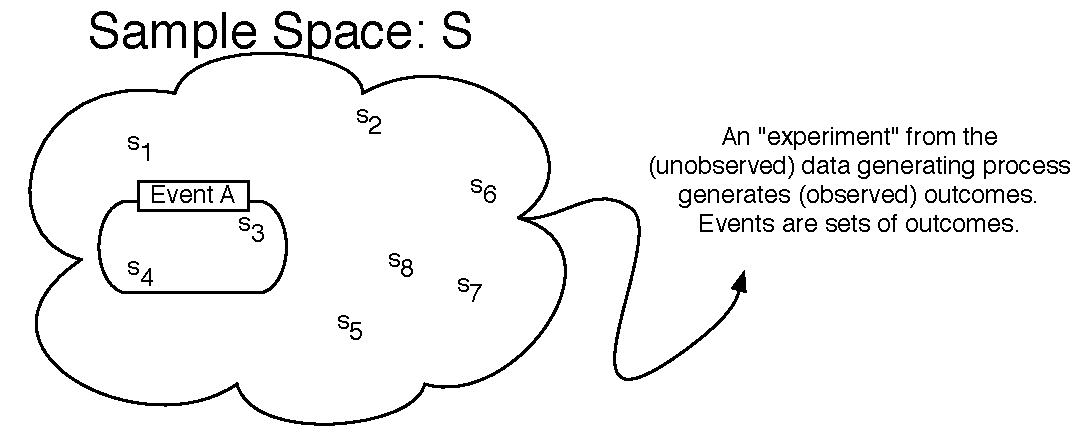
\includegraphics{images/probability.pdf}
\caption[\label{fig:prob-image}Probablity as a Measure]{\label{fig:prob-image}Probablity as a Measure\footnotemark{}}
\end{figure}
\footnotetext{Images of Probability and Random Variables drawn by Shiro Kuriwaki and inspired by Blitzstein and Morris}

\hypertarget{probability-definitions-formal-and-informal}{%
\subsection*{Probability Definitions: Formal and Informal}\label{probability-definitions-formal-and-informal}}
\addcontentsline{toc}{subsection}{Probability Definitions: Formal and Informal}

Many things in the world are uncertain. In everyday speech, we say that we are \emph{uncertain} about the outcome of random events. Probability is a formal model of uncertainty which provides a measure of uncertainty governed by a particular set of rules (Figure \ref{fig:prob-image}). A different model of uncertainty would, of course, have a set of rules different from anything we discuss here. Our focus on probability is justified because it has proven to be a particularly useful model of uncertainty.

\textbf{Probability Distribution Function}: a mapping of each event in the sample space \(S\) to the real numbers that satisfy the following three axioms (also called Kolmogorov's Axioms).

Formally,

\BeginKnitrBlock{definition}[Probability]
\protect\hypertarget{def:unnamed-chunk-66}{}{\label{def:unnamed-chunk-66} \iffalse (Probability) \fi{} }
Probability is a function that maps events to a real number, obeying the axioms of probability.
\EndKnitrBlock{definition}

The axioms of probability make sure that the separate events add up in terms of probability, and -- for standardization purposes -- that they add up to 1.

\BeginKnitrBlock{definition}[Axioms of Probability]
\protect\hypertarget{def:unnamed-chunk-67}{}{\label{def:unnamed-chunk-67} \iffalse (Axioms of Probability) \fi{} }

\begin{enumerate}
\def\labelenumi{\arabic{enumi}.}
\tightlist
\item
  For any event \(A\), \(P(A)\ge 0\).
\item
  \(P(S)=1\)
\item
  The Countable Additivity Axiom: For any sequence of \emph{disjoint} (mutually exclusive) events \(A_1,A_2,\ldots\) (of which there may be infinitely many), \[P\left( \bigcup\limits_{i=1}^k
  A_i\right)=\sum\limits_{i=1}^k P(A_i)\]
\end{enumerate}

The last axiom is an extension of a union to infinite sets. When there are only two events in the space, it boils down to:

\begin{align*}
P(A_1 \cup A_2) = P(A_1) + P(A_2) \quad\text{for disjoint } A_1, A_2
\end{align*}
\EndKnitrBlock{definition}

\hypertarget{probability-operations}{%
\subsection*{Probability Operations}\label{probability-operations}}
\addcontentsline{toc}{subsection}{Probability Operations}

Using these three axioms, we can define all of the common rules of probability.

\begin{enumerate}
\def\labelenumi{\arabic{enumi}.}
\tightlist
\item
  \(P(\emptyset)=0\)
\item
  For any event \(A\), \(0\le P(A) \le 1\).
\item
  \(P({A}^C)=1-P(A)\)
\item
  If \(A\subset B\) (\(A\) is a subset of \(B\)), then \(P(A)\le P(B)\).
\item
  For \emph{any} two events \(A\) and \(B\), \(P(A\cup B)=P(A)+P(B)-P(A\cap B)\)
\item
  Boole's Inequality: For any sequence of \(n\) events (which need not be disjoint) \(A_1,A_2,\ldots,A_n\), then \(P\left( \bigcup\limits_{i=1}^n A_i\right) \leq \sum\limits_{i=1}^n P(A_i)\).
\end{enumerate}

\BeginKnitrBlock{example}[Probability]
\protect\hypertarget{exm:prob}{}{\label{exm:prob} \iffalse (Probability) \fi{} }
Assume we have an evenly-balanced, six-sided die.

Then,

\begin{enumerate}
\def\labelenumi{\arabic{enumi}.}
\tightlist
\item
  Sample space S =
\item
  \(P(1)=\cdots=P(6)=\)
\item
  \(P(\emptyset)=P(7)=\)
\item
  \(P\left( \{ 1, 3, 5 \} \right)=\)
\item
  \(P\left( \{ 1, 2 \}^C \right)= P\left( \{ 3, 4, 5, 6 \}\right)=\)
\item
  Let \(A=\{ 1,2,3,4,5 \}\subset S\). Then \(P(A)=5/6<P(S)=\)
\item
  Let \(A=\{ 1, 2, 3 \}\) and \(B=\{ 2, 4, 6 \}\). Then \(A\cup B\)? \(A\cap B\)? \(P(A \cup B)\)?
\end{enumerate}
\EndKnitrBlock{example}

\BeginKnitrBlock{exercise}[Probability]
\protect\hypertarget{exr:prob1}{}{\label{exr:prob1} \iffalse (Probability) \fi{} }
Suppose you had a pair of four-sided dice. You sum the results from a single toss. Let us call this sum, or the outcome, X.

\begin{enumerate}
\def\labelenumi{\arabic{enumi}.}
\item
  What is \(P(X = 5)\), \(P(X = 3)\), \(P(X = 6)\)?
\item
  What is \(P(X=5 \cup X = 3)^C\)?
\end{enumerate}
\EndKnitrBlock{exercise}

\hypertarget{conditional-probability-and-bayes-rule}{%
\section{Conditional Probability and Bayes Rule}\label{conditional-probability-and-bayes-rule}}

\textbf{Conditional Probability}: The conditional probability \(P(A|B)\) of an event \(A\) is the probability of \(A\), given that another event \(B\) has occurred. Conditional probability allows for the inclusion of other information into the calculation of the probability of an event. It is calculated as

\[P(A|B)=\frac{P(A\cap B)}{P(B)}\]

Note that conditional probabilities are probabilities and must also follow the Kolmagorov axioms of probability.

\BeginKnitrBlock{example}[Conditional Probability 1]
\protect\hypertarget{exm:condprobexm1}{}{\label{exm:condprobexm1} \iffalse (Conditional Probability 1) \fi{} }
Assume \(A\) and \(B\) occur with the following frequencies: \(\quad\)

\begin{longtable}[]{@{}lcc@{}}
\toprule
& \(A\) & \(A^c\)\tabularnewline
\midrule
\endhead
\(B\) & \(n_{ab}\) & \(n_{a^cb}\)\tabularnewline
\(B^C\) & \(n_{ab^c}\) & \(n_{(ab)^c}\)\tabularnewline
\bottomrule
\end{longtable}

and let \(n_{ab}+n_{a^Cb}+n_{ab^C}+n_{(ab)^C}=N\). Then

\begin{enumerate}
\def\labelenumi{\arabic{enumi}.}
\tightlist
\item
  \(P(A)=\)
\item
  \(P(B)=\)
\item
  \(P(A\cap B)=\)
\item
  \(P(A|B)= \frac{P(A\cap B)}{P(B)}=\)
\item
  \(P(B|A)= \frac{P(A\cap B)}{P(A)}=\)
\end{enumerate}
\EndKnitrBlock{example}

\BeginKnitrBlock{example}[Conditional Probability 2]
\protect\hypertarget{exm:condprobexm2}{}{\label{exm:condprobexm2} \iffalse (Conditional Probability 2) \fi{} }
A six-sided die is rolled. What is the probability of a 1, given the outcome is an odd number?
\EndKnitrBlock{example}

You could rearrange the fraction to highlight how a joint probability could be expressed as the product of a conditional probability.

\BeginKnitrBlock{definition}[Multiplicative Law of Probability]
\protect\hypertarget{def:unnamed-chunk-68}{}{\label{def:unnamed-chunk-68} \iffalse (Multiplicative Law of Probability) \fi{} }
The probability of the intersection of two events \(A\) and \(B\) is \(P(A\cap B)=P(A)P(B|A)=P(B)P(A|B)\) which follows directly from the definition of conditional probability. More generally,

\[P(A_1\cap \cdots\cap A_k) = P(A_k| A_{k-1}\cap \cdots \cap A_1)\times P(A_{k-1}|A_{k-2}\cap \cdots A_1) \times \ldots \times P(A_2|A_1)\times P(A_1)\]

Sometimes it is easier to calculate these conditional probabilities and sum them than it is to calculate \(P(A)\) directly.
\EndKnitrBlock{definition}

\BeginKnitrBlock{definition}[Law of Total Probability]
\protect\hypertarget{def:unnamed-chunk-69}{}{\label{def:unnamed-chunk-69} \iffalse (Law of Total Probability) \fi{} }Let \(S\) be the sample space of some experiment and let the disjoint \(k\) events \(B_1,\ldots,B_k\) partition \(S\), such that \(P(B_1\cup ... \cup B_k) = P(S) = 1\). If \(A\) is some other event in \(S\), then the events \(A\cap B_1, A\cap B_2, \ldots, A\cap B_k\) will form a partition of \(A\) and we can write \(A\) as \[A=(A\cap B_1)\cup\cdots\cup (A\cap B_k)\].

Since the \(k\) events are disjoint,

\begin{eqnarray*}
P(A)&=&\sum\limits_{i=1}^k P(A \cap B_i)\\
      &=&\sum\limits_{i=1}^k P(B_i)P(A|B_i)
\end{eqnarray*}
\EndKnitrBlock{definition}

\textbf{Bayes Rule}: Assume that events \(B_1,\ldots,B_k\) form a partition of the space \(S\). Then by the Law of Total Probability

\[P(B_j|A)= \frac{P(A \cap B_j)} {P(A)} = \frac{P(B_j) P(A|B_j)}{\sum\limits_{i=1}^k P(B_i)P(A|B_i)}\]

If there are only two states of \(B\), then this is just
\[P(B_1|A)=\frac{P(B_1)P(A|B_1)} {P(B_1)P(A|B_1)+P(B_2)P(A|B_2)}\]

Bayes' rule determines the posterior probability of a state \(P(B_j|A)\) by calculating the probability \(P(A \cap B_j)\) that both the event \(A\) and the state \(B_j\) will occur and dividing it by the probability that the event will occur regardless of the state (by summing across all \(B_i\)). The states could be something like Normal/Defective, Healthy/Diseased, Republican/Democrat/Independent, etc. The event on which one conditions could be something like a sampling from a batch of components, a test for a disease, or a question about a policy position.

\textbf{Prior and Posterior Probabilities}: Above, \(P(B_1)\) is often called the prior probability, since it's the probability of \(B_1\) before anything else is known. \(P(B_1|A)\) is called the posterior probability, since it's the probability after other information is taken into account.

\BeginKnitrBlock{example}[Bayes' Rule]
\protect\hypertarget{exm:bayesrule}{}{\label{exm:bayesrule} \iffalse (Bayes' Rule) \fi{} }
In a given town, 40\% of the voters are Democrat and 60\% are Republican. The president's budget is supported by 50\% of the Democrats and 90\% of the Republicans. If a randomly (equally likely) selected voter is found to support the president's budget, what is the probability that they are a Democrat?
\EndKnitrBlock{example}

\BeginKnitrBlock{exercise}[Conditional Probability]
\protect\hypertarget{exr:condprobexr}{}{\label{exr:condprobexr} \iffalse (Conditional Probability) \fi{} }

Assume that 2\% of the population of the U.S. are members of some extremist militia group. We develop a survey that positively classifies someone as being a member of a militia group given that they are a member 95\% of the time and negatively classifies someone as not being a member of a militia group given that they are not a member 97\% of the time. What is the probability that someone positively classified as being a member of a militia group is actually a militia member?
\EndKnitrBlock{exercise}

\hypertarget{independence}{%
\section{Independence}\label{independence}}

\BeginKnitrBlock{definition}[Independence]
\protect\hypertarget{def:unnamed-chunk-70}{}{\label{def:unnamed-chunk-70} \iffalse (Independence) \fi{} } If the occurrence or nonoccurrence of either events \(A\) and \(B\) have no effect on the occurrence or nonoccurrence of the other, then \(A\) and \(B\) are independent.
\EndKnitrBlock{definition}

If \(A\) and \(B\) are independent, then

\begin{enumerate}
\def\labelenumi{\arabic{enumi}.}
\tightlist
\item
  \(P(A|B)=P(A)\)
\item
  \(P(B|A)=P(B)\)
\item
  \(P(A\cap B)=P(A)P(B)\)
\item
  More generally than the above, \(P(\bigcap_{i=1}^k A_i) = \prod_{i = 1}^K P(A_i)\)
\end{enumerate}

Are mutually exclusive events independent of each other?

No.~If A and B are mutually exclusive, then they cannot happen simultaneously. If we know that A occurred, then we know that B couldn't have occurred. Because of this, A and B aren't independent.

\textbf{Pairwise Independence}: A set of more than two events \(A_1, A_2, \dots, A_k\) is pairwise independent if \(P(A_i\cap A_j)=P(A_i)P(A_j)\), \(\forall i\neq j\). Note that this does \textbf{not} necessarily imply joint independence.

\textbf{Conditional Independence}: If \(A\) and \(B\) are independent once you know the occurrence of a third event \(C\), then \(A\) and \(B\) are conditionally independent (conditional on \(C\)):

\begin{enumerate}
\def\labelenumi{\arabic{enumi}.}
\tightlist
\item
  \(P(A|B \cap C)=P(A|C)\)
\item
  \(P(B|A \cap C)=P(B|C)\)
\item
  \(P(A\cap B|C)=P(A|C)P(B|C)\)
\end{enumerate}

Just because two events are conditionally independent does not mean that they are independent. Actually it is hard to think of real-world things that are ``unconditionally'' independent. That's why it's always important to ask about a finding: What was it conditioned on? For example, suppose that a graduate school admission decisions are done by only one professor, who picks a group of 50 bright students and flips a coin for each student to generate a class of about 25 students. Then the the probability that two students get accepted are conditionally independent, because they are determined by two separate coin tosses. However, this does not mean that their admittance is not completely independent. Knowing that student \(A\) got in gives us information about whether student \(B\) got in, if we think that the professor originally picked her pool of 50 students by merit.

Perhaps more counter-intuitively: If two events are already independent, then it might seem that no amount of ``conditioning'' will make them dependent. But this is not always so. For example\footnote{Example taken from Blitzstein and Hwang, Example 2.5.10}, suppose I only get a call from two people, Alice and Bob. Let \(A\) be the event that Alice calls, and \(B\) be the event that Bob calls. Alice and Bob do not communicate, so \(P(A \mid B) = P(A).\) But now let \(C\) be the event that your phone rings. For conditional independence to hold here, then \(P(A \mid C)\) must be equal to \(P(A \mid B \cap C).\) But this is not true -- \(A \mid C\) may or may not be true, but \(P(A \mid B \cap C)\) certainly is true.

\hypertarget{random-variables}{%
\section{Random Variables}\label{random-variables}}

Most questions in the social sciences involve events, rather than numbers per se. To analyze and reason about events quantitatively, we need a way of mapping events to numbers. A random variable does exactly that.

\begin{figure}
\centering
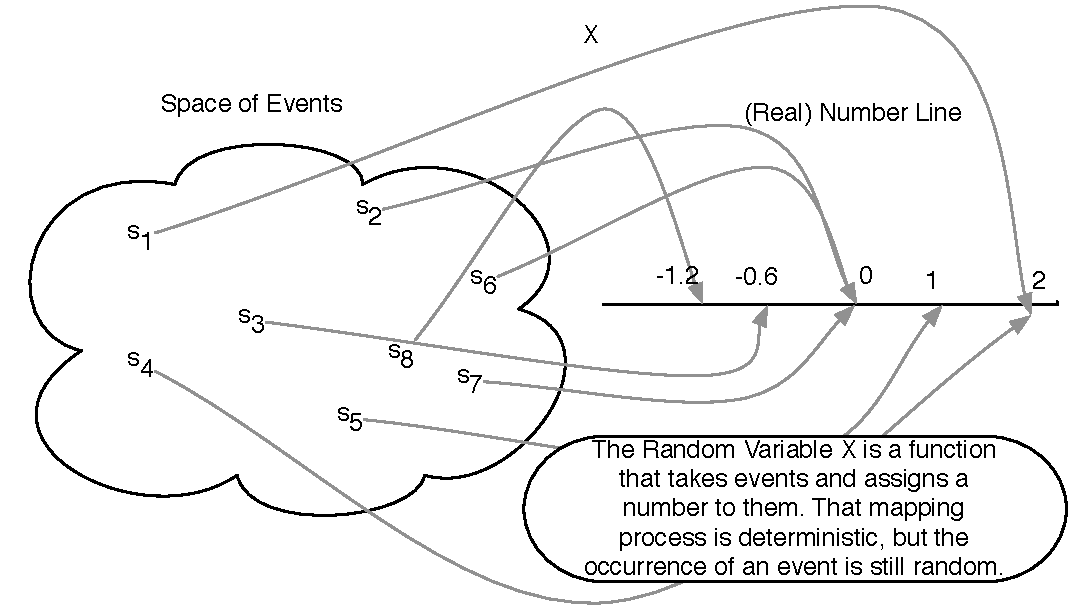
\includegraphics{images/rv.pdf}
\caption{\label{fig:rv-image}The Random Variable as a Real-Valued Function}
\end{figure}

\BeginKnitrBlock{definition}[Random Variable]
\protect\hypertarget{def:unnamed-chunk-71}{}{\label{def:unnamed-chunk-71} \iffalse (Random Variable) \fi{} }
A random variable is a measurable function \(X\) that maps from the sample space \(S\) to the set of real numbers \(R.\) It assigns a real number to every outcome \(s \in S\).
\EndKnitrBlock{definition}

Figure \ref{fig:rv-image} shows a image of the function. It might seem strange to define a random variable as a function -- which is neither random nor variable. The randomness comes from the realization of an event from the sample space \(s\).

\textbf{Randomness} means that the outcome of some experiment is not deterministic, i.e.~there is some probability (\(0 < P(A) < 1\)) that the event will occur.

The support of a random variable is all values for which there is a positive probability of occurrence.

Example: Flip a fair coin two times. What is the sample space?

A random variable must map events to the real line. For example, let a random variable \(X\) be the number of heads. The event \((H, H)\) gets mapped to 2 \(X(s) = 2\), and the events \(\{(H, T), (T, H)\}\) gets mapped to 1 \((X(s) = 1)\), the event \((T, T)\) gets mapped to 0 \((X(s) = 0)\).

What are other possible random variables?

\hypertarget{distributions}{%
\section{Distributions}\label{distributions}}

We now have two main concepts in this section -- probability and random variables. Given a sample space \(S\) and the same experiment, both probability and random variables take events as their inputs. But they output different things (probabilities measure the ``size'' of events, random variables give a number in a way that the analyst chose to define the random variable). How do the two concepts relate?

The concept of distributions is the natural bridge between these two concepts.

\BeginKnitrBlock{definition}[Distribution of a random variable]
\protect\hypertarget{def:unnamed-chunk-72}{}{\label{def:unnamed-chunk-72} \iffalse (Distribution of a random variable) \fi{} }A distribution of a random variable is a function that specifies the probabilities of all events associated with that random variable. There are several types of distributions: A probability mass function for a discrete random variable and probability density function for a continuous random variable.
\EndKnitrBlock{definition}

Notice how the definition of distributions combines two ideas of random variables and probabilities of events. First, the distribution considers a random variable, call it \(X\). \(X\) can take a number of possible numeric values.

\BeginKnitrBlock{example}[Total Number of Occurrences]
\protect\hypertarget{exm:unnamed-chunk-73}{}{\label{exm:unnamed-chunk-73} \iffalse (Total Number of Occurrences) \fi{} }
Consider three binary outcomes, one for each patient recovering from a disease: \(R_i\) denotes the event in which patient \(i\) (\(i = 1, 2, 3\)) recovers from a disease. \(R_1\), \(R_2\), and \(R_3\). How would we represent the total number of people who end up recovering from the disease?
\EndKnitrBlock{example}

\BeginKnitrBlock{solution}
\iffalse{} {Solution. } \fi{}Define the random variable \(X\) be the total number of people (out of three) who recover from the disease. Random variables are functions, that take as an input a set of events (in the sample space \(S\)) and deterministically assigns them to a number of the analyst's choice.
\EndKnitrBlock{solution}

Recall that with each of these numerical values there is a class of \emph{events}. In the previous example, for \(X = 3\) there is one outcome (\(R_1, R_2, R_3\)) and for \(X = 1\) there are multiple (\(\{(R_1, R_2^c, R_3^c), (R_1^c, R_2, R_3^c), (R_1^c, R_2^c, R_3), \}\)). Now, the thing to notice here is that each of these events naturally come with a probability associated with them. That is, \(P(R_1, R_2, R_3)\) is a number from 0 to 1, as is \(P(R_1, R_2^c, R_3^c)\). These all have probabilities because they are in the sample space \(S\). The function that tells us these probabilities that are associated with a numerical value of a random variable is called a distribution.

In other words, a random variable \(X\) \emph{induces a probability distribution} \(P\) (sometimes written \(P_X\) to emphasize that the probability density is about the r.v. \(X\))

\hypertarget{discrete-random-variables}{%
\subsection*{Discrete Random Variables}\label{discrete-random-variables}}
\addcontentsline{toc}{subsection}{Discrete Random Variables}

The formal definition of a random variable is easier to given by separating out two cases: discrete random variables when the numeric summaries of the events are discrete, and continuous random variables when they are continuous.

\BeginKnitrBlock{definition}[Discrete Random Variable]
\protect\hypertarget{def:unnamed-chunk-75}{}{\label{def:unnamed-chunk-75} \iffalse (Discrete Random Variable) \fi{} }\(X\) is a discrete random variable if it can assume only a finite or countably infinite number of distinct values. Examples: number of wars per year, heads or tails.
\EndKnitrBlock{definition}

The distribution of a discrete r.v. is a PMF:

\BeginKnitrBlock{definition}[Probability Mass Function]
\protect\hypertarget{def:unnamed-chunk-76}{}{\label{def:unnamed-chunk-76} \iffalse (Probability Mass Function) \fi{} }
For a discrete random variable \(X\), the probability mass function (Also referred to simply as the ``probability distribution.'') (PMF), \(p(x)=P(X=x)\), assigns probabilities to a countable number of distinct \(x\) values such that

\begin{enumerate}
\def\labelenumi{\arabic{enumi}.}
\tightlist
\item
  \(0\le p(x)\le 1\)
\item
  \(\sum\limits_y p(x)=1\)
\end{enumerate}
\EndKnitrBlock{definition}

Example: For a fair six-sided die, there is an equal probability of rolling any number. Since there are six sides, the probability mass function is then \(p(y)=1/6\) for \(y=1,\ldots,6\), 0 otherwise.\}

\begin{comment}
\parbox[t]{1in}{\, \epsffile{diepmf.eps}}
\end{comment}

In a discrete random variable, \textbf{cumulative density function} (Also referred to simply as the ``cumulative distribution'' or previously as the ``density function''), \(F(x)\) or \(P(X\le x)\), is the probability that \(X\) is less than or equal to some value \(x\), or \[P(X\le x)=\sum\limits_{i\le x} p(i)\]

Properties a CDF must satisfy:

\begin{enumerate}
\def\labelenumi{\arabic{enumi}.}
\tightlist
\item
  \(F(x)\) is non-decreasing in \(x\).
\item
  \(\lim\limits_{x \to -\infty} F(x) = 0\) and \(\lim\limits_{x \to \infty} F(x) = 1\)
\item
  \(F(x)\) is right-continuous.
\end{enumerate}

Note that \(P(X > x) = 1 - P(X \le x)\).

\BeginKnitrBlock{example}
\protect\hypertarget{exm:unnamed-chunk-77}{}{\label{exm:unnamed-chunk-77} }For a fair die with its value as \(Y\), What are the following?

\begin{enumerate}
\def\labelenumi{\arabic{enumi}.}
\tightlist
\item
  \(P(Y\le 1)\)
\item
  \(P(Y\le 3)\)
\item
  \(P(Y\le 6)\)
\end{enumerate}
\EndKnitrBlock{example}

\hypertarget{continuous-random-variables}{%
\subsection*{Continuous Random Variables}\label{continuous-random-variables}}
\addcontentsline{toc}{subsection}{Continuous Random Variables}

We also have a similar definition for \emph{continuous} random variables.

\BeginKnitrBlock{definition}[Continuous Random Variable]
\protect\hypertarget{def:unnamed-chunk-78}{}{\label{def:unnamed-chunk-78} \iffalse (Continuous Random Variable) \fi{} }
\(X\) is a continuous random variable if there exists a nonnegative function \(f(x)\) defined for all real \(x\in (-\infty,\infty)\), such that for any interval \(A\), \(P(X\in A)=\int\limits_A f(x)dx\). Examples: age, income, GNP, temperature.
\EndKnitrBlock{definition}

\BeginKnitrBlock{definition}[Probability Density Function]
\protect\hypertarget{def:unnamed-chunk-79}{}{\label{def:unnamed-chunk-79} \iffalse (Probability Density Function) \fi{} }
The function \(f\) above is called the probability density function (pdf) of \(X\) and must satisfy
\[f(x)\ge 0\]
\[\int\limits_{-\infty}^\infty f(x)dx=1\]

Note also that \(P(X = x)=0\) --- i.e., the probability of any point \(y\) is zero.
\EndKnitrBlock{definition}

\begin{comment}
\item[] \parbox[t]{4.5in}{Example: $f(y)=1, \quad 0\le y \le1$}\parbox{1.5in}{\hfill
\epsffile{contpdf.eps}}
\end{comment}

For both discrete and continuous random variables, we have a unifying concept of another measure: the cumulative distribution:

\BeginKnitrBlock{definition}[Cumulative Density Function]
\protect\hypertarget{def:unnamed-chunk-80}{}{\label{def:unnamed-chunk-80} \iffalse (Cumulative Density Function) \fi{} }Because the probability that a continuous random variable will assume any particular value is zero, we can only make statements about the probability of a continuous random variable being within an interval. The cumulative distribution gives the probability that \(Y\) lies on the interval \((-\infty,y)\) and is defined as \[F(x)=P(X\le x)=\int\limits_{-\infty}^x f(s)ds\] Note that \(F(x)\) has similar properties with continuous distributions as it does with discrete - non-decreasing, continuous (not just right-continuous), and \(\lim\limits_{x \to -\infty} F(x) = 0\) and \(\lim\limits_{x \to \infty} F(x) = 1\).
\EndKnitrBlock{definition}

We can also make statements about the probability of \(Y\) falling in an interval \(a\le y\le b\).
\[P(a\le x\le b)=\int\limits_a^b f(x)dx\]

The PDF and CDF are linked by the integral: The CDF of the integral of the PDF: \[f(x) = F'(x)=\frac{dF(x)}{dx}\]

\BeginKnitrBlock{example}
\protect\hypertarget{exm:unnamed-chunk-81}{}{\label{exm:unnamed-chunk-81} }
For \(f(y)=1, \quad 0<y<1\), find: (1) The CDF \(F(y)\) and (2) The probability \(P(0.5<y<0.75)\).
\EndKnitrBlock{example}

\hypertarget{joint-distributions}{%
\section{Joint Distributions}\label{joint-distributions}}

Often, we are interested in two or more random variables defined on the same sample space. The distribution of these variables is called a joint distribution. Joint distributions can be made up of any combination of discrete and continuous random variables.

\textbf{Joint Probability Distribution}: If both \(X\) and \(Y\) are random variable, their joint probability mass/density function assigns probabilities to each pair of outcomes

Discrete:

\[p(x, y) = P(X = x, Y = y)\]

such that \(p(x,y) \in [0,1]\) and \[\sum\sum p(x,y) = 1\]

Continuous:

\[f(x,y);P((X,Y) \in A) = \int\!\!\!\int_A f(x,y)dx dy \]

s.t. \(f(x,y)\ge 0\) and

\[\int_{-\infty}^\infty\int_{-\infty}^\infty f(x,y)dxdy = 1\]

If X and Y are independent, then \(P(X=x,Y=y) = P(X=x)P(Y=y)\) and \(f(x,y) = f(x)f(y)\)

\textbf{Marginal Probability Distribution}: probability distribution of only one of the two variables (ignoring information about the other variable), we can obtain the marginal distribution by summing/integrating across the variable that we don't care about:

\begin{itemize}
\tightlist
\item
  Discrete: \(p_X(x) = \sum_i p(x, y_i)\)
\item
  Continuous: \(f_X(x) = \int_{-\infty}^\infty f(x,y)dy\)
\end{itemize}

\textbf{Conditional Probability Distribution}: probability distribution for one variable, holding the other variable fixed. Recalling from the previous lecture that \(P(A|B)=\frac{P(A\cap B)}{P(B)}\), we can write the conditional distribution as

\begin{itemize}
\tightlist
\item
  Discrete: \(p_{Y|X}(y|x) = \frac{p(x,y)}{p_X(x)}, \quad p_X(x) > 0\)
\item
  Continuous: \(f_{Y|X}(y|x) = \frac{f(x,y)}{f_X(x)},\quad f_X(x) > 0\)
\end{itemize}

\BeginKnitrBlock{exercise}[Discrete Outcomes]
\protect\hypertarget{exr:unnamed-chunk-82}{}{\label{exr:unnamed-chunk-82} \iffalse (Discrete Outcomes) \fi{} }Suppose we are interested in the outcomes of flipping a coin and rolling a 6-sided die at the same time. The sample space for this process contains 12 elements: \[\{(H, 1), (H, 2), (H, 3), (H, 4), (H, 5), (H, 6), (T, 1), (T, 2), (T, 3), (T, 4), (T, 5), (T, 6)\}\] We can define two random variables \(X\) and \(Y\) such that \(X = 1\) if heads and \(X = 0\) if tails, while \(Y\) equals the number on the die.

We can then make statements about the joint distribution of \(X\) and \(Y\). What are the following?

\begin{enumerate}
\def\labelenumi{\arabic{enumi}.}
\tightlist
\item
  \(P(X=x)\)
\item
  \(P(Y=y)\)
\item
  \(P(X=x, Y=y)\)
\item
  \(P(X=x|Y=y)\)
\item
  Are X and Y independent?
\end{enumerate}
\EndKnitrBlock{exercise}

\hypertarget{expectation}{%
\section{Expectation}\label{expectation}}

We often want to summarize some characteristics of the distribution of a random variable. The most important summary is the expectation (or expected value, or mean), in which the possible values of a random variable are weighted by their probabilities.

\BeginKnitrBlock{definition}[Expectation of a Discrete Random Variable]
\protect\hypertarget{def:unnamed-chunk-83}{}{\label{def:unnamed-chunk-83} \iffalse (Expectation of a Discrete Random Variable) \fi{} }The expected value of a discrete random variable \(Y\) is \[E(Y)=\sum\limits_{y} y P(Y=y)= \sum\limits_{y} y p(y)\]\\
In words, it is the weighted average of all possible values of \(Y\), weighted by the probability that \(y\) occurs. It is not necessarily the number we would expect \(Y\) to take on, but the average value of \(Y\) after a large number of repetitions of an experiment.
\EndKnitrBlock{definition}

\BeginKnitrBlock{example}[Expectation of a Discrete Random Variable]
\protect\hypertarget{exm:expectdiscrete}{}{\label{exm:expectdiscrete} \iffalse (Expectation of a Discrete Random Variable) \fi{} }

What is the expectation of a fair, six-sided die?
\EndKnitrBlock{example}

\textbf{Expectation of a Continuous Random Variable}: The expected
value of a continuous random variable is similar in concept to that of
the discrete random variable, except that instead of summing using
probabilities as weights, we integrate using the density to weight.
Hence, the expected value of the continuous variable \(Y\) is defined by
\[E(Y)=\int\limits_{y} y f(y) dy\]

\BeginKnitrBlock{example}[Expectation of a Continuous Random Variable]
\protect\hypertarget{exm:expectconti}{}{\label{exm:expectconti} \iffalse (Expectation of a Continuous Random Variable) \fi{} }

Find \(E(Y)\) for \(f(y)=\frac{1}{1.5}, \quad 0<y<1.5\).
\EndKnitrBlock{example}

\hypertarget{expected-value-of-a-function}{%
\subsection*{Expected Value of a Function}\label{expected-value-of-a-function}}
\addcontentsline{toc}{subsection}{Expected Value of a Function}

Remember: An Expected Value is a type of weighted average. We can extend this to composite functions. For random variable \(Y\),

If \(Y\) is Discrete with PMF \(p(y)\),

\[E[g(Y)]=\sum\limits_y g(y)p(y)\]

If \(Y\) is Continuous with PDF \(f(y)\),

\[E[g(Y)]=\int\limits_{-\infty}^\infty g(y)f(y)dy\]

\hypertarget{properties-of-expected-values}{%
\subsection*{Properties of Expected Values}\label{properties-of-expected-values}}
\addcontentsline{toc}{subsection}{Properties of Expected Values}

Dealing with Expectations is easier when the thing inside is a sum. The intuition behind this that Expectation is an integral, which is a type of sum.

\begin{enumerate}
\def\labelenumi{\arabic{enumi}.}
\tightlist
\item
  Expectation of a constant is a constant \[E(c)=c\]
\item
  Constants come out \[E(c g(Y))= c E(g(Y))\]
\item
  Expectation is Linear \[E(g(Y_1) + \cdots + g(Y_n))=E(g(Y_1)) +\cdots+E(g(Y_n)),\] regardless of independence
\item
  Expected Value of Expected Values: \[E(E(Y)) = E(Y)\] (because the expected value of a random variable is a constant)
\end{enumerate}

Finally, if \(X\) and \(Y\) are independent, even products are easy:

\[E(XY) = E(X)E(Y)\]

\textbf{Conditional Expectation}: With joint distributions, we are often interested in the expected value of a variable \(Y\) if we could hold the other variable \(X\) fixed. This is the conditional expectation of \(Y\) given \(X = x\):

\begin{enumerate}
\def\labelenumi{\arabic{enumi}.}
\tightlist
\item
  \(Y\) discrete: \(E(Y|X = x) = \sum_y yp_{Y|X}(y|x)\)
\item
  \(Y\) continuous: \(E(Y|X = x) = \int_y yf_{Y|X}(y|x)dy\)
\end{enumerate}

The conditional expectation is often used for prediction when one knows the value of \(X\) but not \(Y\)

\hypertarget{variance-and-covariance}{%
\section{Variance and Covariance}\label{variance-and-covariance}}

We can also look at other summaries of the distribution, which build on the idea of taking expectations. Variance tells us about the ``spread'' of the distribution; it is the expected value of the squared deviations from the mean of the distribution. The standard deviation is simply the square root of the variance.

\BeginKnitrBlock{definition}[Variance]
\protect\hypertarget{def:unnamed-chunk-84}{}{\label{def:unnamed-chunk-84} \iffalse (Variance) \fi{} }The Variance of a Random Variable \(Y\) is

\[\text{Var}(Y) = E[(Y - E(Y))^2] =  E(Y^2)-[E(Y)]^2\]

The Standard Deviation is the square root of the variance : \[SD(Y) = \sigma_Y= \sqrt{\text{Var}(Y)}\]
\EndKnitrBlock{definition}

\BeginKnitrBlock{example}[Variance]
\protect\hypertarget{exm:var}{}{\label{exm:var} \iffalse (Variance) \fi{} }

Given the following PMF:
\[f(x) =  \begin{cases}
              \frac{3!}{x!(3-x)!}(\frac{1}{2})^3 \quad x = 0,1,2,3\\
               0 \quad otherwise
            \end{cases}
               \]

What is \(\text{Var}(x)\)?

\textbf{Hint:} First calculate \(E(X)\) and \(E(X^2)\)
\EndKnitrBlock{example}

\BeginKnitrBlock{definition}[Covariance and Correlation]
\protect\hypertarget{def:unnamed-chunk-85}{}{\label{def:unnamed-chunk-85} \iffalse (Covariance and Correlation) \fi{} }
The covariance measures the degree to which two random variables vary together; if the covariance between \(X\) and \(Y\) is positive, X tends to be larger than its mean when Y is larger than its mean.

\[\text{Cov}(X,Y) = E[(X - E(X))(Y - E(Y))] \]
We can also write this as

\begin{align*}
\text{Cov}(X,Y) &= E\left(XY - XE(Y) - E(X)Y + E(X)E(Y)\right)\\
&= E(XY) - E(X)E(Y) - E(X)E(Y) + E(X)E(Y)\\
&= E(XY) - E(X)E(Y)
\end{align*}
\EndKnitrBlock{definition}

The covariance of a variable with itself is the variance of that variable.

The Covariance is unfortunately hard to interpret in magnitude. The correlation is a standardized version of the covariance, and always ranges from -1 to 1.

\BeginKnitrBlock{definition}[Correlation]
\protect\hypertarget{def:unnamed-chunk-86}{}{\label{def:unnamed-chunk-86} \iffalse (Correlation) \fi{} }The correlation coefficient is the covariance divided by the standard deviations of \(X\) and \(Y\). It is a unitless measure and always takes on values in the interval \([-1,1]\).

\[\text{Corr}(X, Y) = \frac{\text{Cov}(X,Y)}{\sqrt{\text{Var}(X)\text{Var}(Y)}} = \frac{\text{Cov}(X,Y)}{SD(X)SD(Y)}\]
\EndKnitrBlock{definition}

\textbf{\emph{Properties of Variance and Covariance:}}

\begin{enumerate}
\def\labelenumi{\arabic{enumi}.}
\tightlist
\item
  \(\text{Var}(c) = 0\)
\item
  \(\text{Var}(cY) = c^2 \text{Var}(Y)\)
\item
  \(\text{Cov}(Y,Y) = \text{Var}(Y)\)
\item
  \(\text{Cov}(X,Y) = \text{Cov}(Y,X)\)
\item
  \(\text{Cov}(aX,bY) = ab \text{Cov}(X,Y)\)
\item
  \(\text{Cov}(X+a,Y) = \text{Cov}(X,Y)\)
\item
  \(\text{Cov}(X+Z,Y+W) = \text{Cov}(X,Y) + \text{Cov}(X,W) + \text{Cov}(Z,Y) + \text{Cov}(Z,W)\)
\item
  \(\text{Var}(X+Y) = \text{Var}(X) + \text{Var}(Y) + 2\text{Cov}(X,Y)\)
\end{enumerate}

\BeginKnitrBlock{exercise}[Expectation and Variance]
\protect\hypertarget{exr:expvar}{}{\label{exr:expvar} \iffalse (Expectation and Variance) \fi{} }
Suppose we have a PMF with the following characteristics:
\begin{eqnarray*}
  P(X = -2) = \frac{1}{5}\\
  P(X = -1) = \frac{1}{6}\\
  P(X = 0) = \frac{1}{5}\\
  P(X = 1) = \frac{1}{15}\\
  P(X = 2) = \frac{11}{30}
\end{eqnarray*}

\begin{enumerate}
\def\labelenumi{\arabic{enumi}.}
\tightlist
\item
  Calculate the expected value of X
\end{enumerate}

Define the random variable \(Y = X^2\).

\begin{enumerate}
\def\labelenumi{\arabic{enumi}.}
\setcounter{enumi}{1}
\item
  Calculate the expected value of Y. (Hint: It would help to derive the PMF of Y first in order to calculate the expected value of Y in a straightforward way)
\item
  Calculate the variance of X.
\end{enumerate}
\EndKnitrBlock{exercise}

\BeginKnitrBlock{exercise}[Expectation and Variance 2]
\protect\hypertarget{exr:expvar2}{}{\label{exr:expvar2} \iffalse (Expectation and Variance 2) \fi{} }

\begin{enumerate}
\def\labelenumi{\arabic{enumi}.}
\tightlist
\item
  Find the expectation and variance
\end{enumerate}

Given the following PDF:
\[f(x) =  \begin{cases}
              \frac{3}{10}(3x - x^2) \quad 0 \leq x \leq 2\\
               0 \quad otherwise
            \end{cases}
               \]
\EndKnitrBlock{exercise}

\BeginKnitrBlock{exercise}[Expectation and Variance 3]
\protect\hypertarget{exr:expvar3}{}{\label{exr:expvar3} \iffalse (Expectation and Variance 3) \fi{} }

\begin{enumerate}
\def\labelenumi{\arabic{enumi}.}
\tightlist
\item
  Find the mean and standard deviation of random variable X. The PDF of this X is as follows:
\end{enumerate}

\[f(x) =  \begin{cases}
              \frac{1}{4}x \quad 0 \leq x \leq 2\\
               \frac{1}{4}(4 - x)  \quad 2 \leq x \leq 4\\
               0 \quad otherwise
            \end{cases}
               \]

\begin{enumerate}
\def\labelenumi{\arabic{enumi}.}
\setcounter{enumi}{1}
\tightlist
\item
  Next, calculate \(P(X < \mu - \sigma)\) Remember, \(\mu\) is the mean and \(\sigma\) is the standard deviation
\end{enumerate}
\EndKnitrBlock{exercise}

\hypertarget{special-distributions}{%
\section{Special Distributions}\label{special-distributions}}

Two \emph{discrete} distributions used often are:

\BeginKnitrBlock{definition}[Binomial Distribution]
\protect\hypertarget{def:unnamed-chunk-87}{}{\label{def:unnamed-chunk-87} \iffalse (Binomial Distribution) \fi{} }\(Y\) is distributed binomial if it represents the number of ``successes'' observed in \(n\) independent, identical ``trials,'' where the probability of success in any trial is \(p\) and the probability of failure is \(q=1-p\).
\EndKnitrBlock{definition}

For any particular sequence of \(y\) successes and \(n-y\) failures, the probability of obtaining that sequence is \(p^y q^{n-y}\) (by the multiplicative law and independence). However, there are \(\binom{n}{y}=\frac{n!}{(n-y)!y!}\) ways of obtaining a sequence with \(y\) successes and \(n-y\) failures. So the binomial distribution is given by \[p(y)=\binom{n}{y}p^y q^{n-y}, \quad y=0,1,2,\ldots,n\] with mean \(\mu=E(Y)=np\) and variance \(\sigma^2=\text{Var}(Y)=npq\).

\BeginKnitrBlock{example}
\protect\hypertarget{exm:unnamed-chunk-88}{}{\label{exm:unnamed-chunk-88} }Republicans vote for Democrat-sponsored bills 2\% of the time. What is the probability that out of 10 Republicans questioned, half voted for a particular Democrat-sponsored bill? What is the mean number of Republicans voting for Democrat-sponsored bills? The variance?
1. \(P(Y=5)=\)
1. \(E(Y)=\)
1. \(\text{Var}(Y)=6\)
\EndKnitrBlock{example}

\begin{comment}
  \parbox{1.5in}{\hfill \epsffile{binopmf.eps}}
  \end{comment}

\BeginKnitrBlock{definition}[Poisson Distribution]
\protect\hypertarget{def:unnamed-chunk-89}{}{\label{def:unnamed-chunk-89} \iffalse (Poisson Distribution) \fi{} }A random variable \(Y\) has a Poisson distribution if

\[P(Y = y)=\frac{\lambda^y}{y!}e^{-\lambda}, \quad y=0,1,2,\ldots, \quad \lambda>0\]

The Poisson has the unusual feature that its expectation equals its variance: \(E(Y)=\text{Var}(Y)=\lambda\). The Poisson distribution is often used to model rare event counts: counts of the number of events that occur during some unit of time. \(\lambda\) is often called the ``arrival rate.''
\EndKnitrBlock{definition}

\BeginKnitrBlock{example}
\protect\hypertarget{exm:unnamed-chunk-90}{}{\label{exm:unnamed-chunk-90} }Border disputes occur between two countries through a Poisson Distribution, at a rate of 2 per month. What is the probability of 0, 2, and less than 5 disputes occurring in a month?
\EndKnitrBlock{example}

\begin{comment}
 \parbox{1.5in}{\hfill \epsffile{poispmf.eps}}
 \end{comment}

Two \emph{continuous} distributions used often are:

\BeginKnitrBlock{definition}[Uniform Distribution]
\protect\hypertarget{def:unnamed-chunk-91}{}{\label{def:unnamed-chunk-91} \iffalse (Uniform Distribution) \fi{} }A random variable \(Y\) has a continuous uniform distribution on the interval \((\alpha,\beta)\) if its density is given by \[f(y)=\frac{1}{\beta-\alpha}, \quad \alpha\le y\le \beta\] The mean and variance of \(Y\) are \(E(Y)=\frac{\alpha+\beta}{2}\) and \(\text{Var}(Y)=\frac{(\beta-\alpha)^2}{12}\).
\EndKnitrBlock{definition}

\BeginKnitrBlock{example}
\protect\hypertarget{exm:unnamed-chunk-92}{}{\label{exm:unnamed-chunk-92} }For \(Y\) uniformly distributed over \((1,3)\), what are the following probabilities?

\begin{enumerate}
\def\labelenumi{\arabic{enumi}.}
\tightlist
\item
  \(P(Y=2)\)
\item
  Its density evaluated at 2, or \(f(2)\)
\item
  \(P(Y \le 2)\)
\item
  \(P(Y > 2)\)
\end{enumerate}
\EndKnitrBlock{example}

\begin{comment}
\parbox{1.5in}{\hfill \epsffile{unifpdf.eps}}
\end{comment}

\BeginKnitrBlock{definition}[Normal Distribution]
\protect\hypertarget{def:unnamed-chunk-93}{}{\label{def:unnamed-chunk-93} \iffalse (Normal Distribution) \fi{} }
A random variable \(Y\) is normally distributed with mean \(E(Y)=\mu\) and variance \(\text{Var}(Y)=\sigma^2\) if its density is

\[f(y)=\frac{1}{\sqrt{2\pi}\sigma}e^{-\frac{(y-\mu)^2}{2\sigma^2}}\]
\EndKnitrBlock{definition}

See Figure \ref{fig:normaldens} are various Normal Distributions with the same \(\mu = 1\) and two versions of the variance.

\begin{figure}
\centering
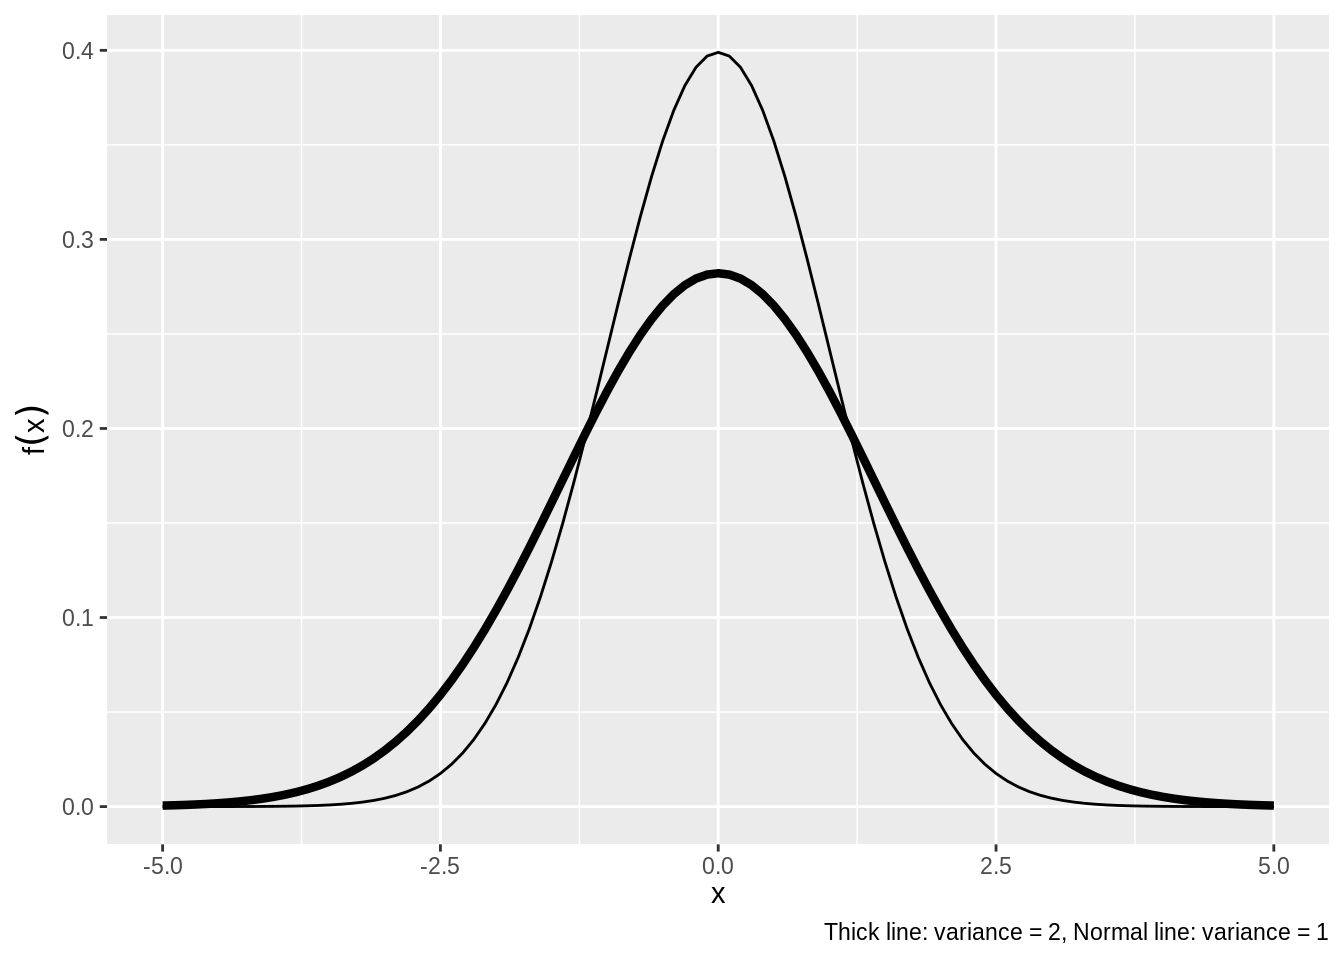
\includegraphics{prefresher_files/figure-latex/normaldens-1.pdf}
\caption{\label{fig:normaldens}Normal Distribution Density}
\end{figure}

\hypertarget{summarizing-observed-events-data}{%
\section{Summarizing Observed Events (Data)}\label{summarizing-observed-events-data}}

So far, we've talked about distributions in a theoretical sense, looking at different properties of random variables. We don't observe random variables; we observe realizations of the random variable. These realizations of events are roughly equivalent to what we mean by ``data''.

\textbf{Sample mean}: This is the most common measure of central tendency, calculated by summing across the observations and dividing by the number of observations.
\[\bar{x} = \frac{1}{n}\sum_{i=1}^{n}x_i\]
The sample mean is an \emph{estimate} of the expected value of a distribution.

\begin{framed}
Example:  
\begin{center}
\begin{tabular}{|l|cccccccccc|}
\hline
X & 6 & 3 & 7 & 5 & 5 & 5 & 6 & 4 & 7 & 2\\
\hline
Y & 1 & 2 & 1 & 2 & 2 & 1 & 2 & 0 & 2 & 0\\
\hline
\end{tabular}
\end{center}

\begin{enumerate}
\item $\bar{x} = $ \hspace{3.1cm} $\bar{y} = $
\item median(x) $ = $ \hspace{1.5cm} median(y) $ = $
\item $m_x = $ \hspace{2.75cm} $m_y =$\\
\end{enumerate}
\end{framed}

\textbf{Dispersion}: We also typically want to know how spread out the data are relative to the center of the observed distribution. There are several ways to measure dispersion.

\textbf{Sample variance}: The sample variance is the sum of the squared deviations from the sample mean, divided by the number of observations minus 1.
\[ \hat{\text{Var}}(X) = \frac{1}{n-1}\sum_{i = 1}^n (x_i - \bar{x})^2\]

Again, this is an \emph{estimate} of the variance of a random variable; we divide by \(n - 1\) instead of \(n\) in order to get an unbiased estimate.

\textbf{Standard deviation}: The sample standard deviation is the square root of the sample variance.
\[ \hat{SD}(X) = \sqrt{\hat{\text{Var}}(X)} = \sqrt{\frac{1}{n-1}\sum_{i = 1}^n (x_i - \bar{x})^2}\]

\begin{framed}
Example: Using table above, calculate: 
\begin{enumerate}
\item $\text{Var}(X) = $ \hspace{1.5cm} $\text{Var}(Y) =$
\item $\SD(X) = $ \hspace{1.65cm} $\SD(Y) =$
\end{enumerate}
\end{framed}

\textbf{Covariance and Correlation}: Both of these quantities measure the degree to which two variables vary together, and are estimates of the covariance and correlation of two random variables as defined above.

\begin{enumerate}
\def\labelenumi{\arabic{enumi}.}
\tightlist
\item
  \textbf{Sample covariance}: \(\hat{\text{Cov}}(X,Y) = \frac{1}{n-1}\sum_{i = 1}^n(x_i - \bar{x})(y_i - \bar{y})\)
\item
  \textbf{Sample correlation}: \(\hat{\text{Corr}} = \frac{\hat{\text{Cov}}(X,Y)}{\sqrt{\hat{\text{Var}}(X)\hat{\text{Var}}(Y)}}\)
\end{enumerate}

\BeginKnitrBlock{example}
\protect\hypertarget{exm:unnamed-chunk-94}{}{\label{exm:unnamed-chunk-94} }Example: Using the above table, calculate the sample versions of:

\begin{enumerate}
\def\labelenumi{\arabic{enumi}.}
\tightlist
\item
  \(\text{Cov}(X,Y)\)
\item
  \(\text{Corr}(X, Y)\)
\end{enumerate}
\EndKnitrBlock{example}

\hypertarget{asymptotic-theory}{%
\section{Asymptotic Theory}\label{asymptotic-theory}}

In theoretical and applied research, asymptotic arguments are often made. In this section we briefly introduce some of this material.

What are asymptotics? In probability theory, asymptotic analysis is the study of limiting behavior. By limiting behavior, we mean the behavior of some random process as the number of observations gets larger and larger.

Why is this important? We rarely know the true process governing the events we see in the social world. It is helpful to understand how such unknown processes theoretically must behave and asymptotic theory helps us do this.

\hypertarget{clt-and-lln}{%
\subsection{CLT and LLN}\label{clt-and-lln}}

We are now finally ready to revisit, with a bit more precise terms, the two pillars of statistical theory we motivated Section \ref{limitsfun} with.

\BeginKnitrBlock{theorem}[Central Limit Theorem (i.i.d. case)]
\protect\hypertarget{thm:clt}{}{\label{thm:clt} \iffalse (Central Limit Theorem (i.i.d. case)) \fi{} }Let \(\{X_n\} = \{X_1, X_2, \ldots\}\) be a sequence of i.i.d. random variables with finite mean (\(\mu\)) and variance (\(\sigma^2\)). Then, the sample mean \(\bar{X}_n = \frac{X_1 + X_2 + \cdots + X_n}{n}\) increasingly converges into a Normal distribution.

\[\frac{\bar{X}_n - \mu}{\sigma / \sqrt{n}} \xrightarrow{d} \text{Normal}(0, 1),\]

Another way to write this as a probability statement is that for all real numbers \(a\),

\[P\left(\frac{\bar{X}_n - \mu}{\sigma/\sqrt{n}} \le a\right) \rightarrow \Phi(a)\]
as \(n\to \infty\), where \[\Phi(x) = \int_{-\infty}^x \frac{1}{\sqrt{2\pi}}e^{-\frac{x^2}{2}} \, dx\] is the CDF of a Normal distribution with mean 0 and variance 1.

This result means that, as \(n\) grows, the distribution of the sample mean \(\bar X_n = \frac{1}{n} (X_1 + X_2 + \cdots + X_n)\) is approximately normal with mean \(\mu\) and standard deviation \(\frac{\sigma}{\sqrt n}\), i.e.,
\[\bar{X}_n \approx \mathcal{N}\bigg(\mu, \frac{\sigma^2}{n}\bigg).\] The standard deviation of \(\bar X_n\) (which is roughly a measure of the precision of \(\bar X_n\) as an estimator of \(\mu\)) decreases at the rate \(1/\sqrt{n}\), so, for example, to increase its precision by \(10\) (i.e., to get one more digit right), one needs to collect \(10^2=100\) times more units of data.

Intuitively, this result also justifies that whenever a lot of small, independent processes somehow combine together to form the realized observations, practitioners often feel comfortable assuming Normality.
\EndKnitrBlock{theorem}

\BeginKnitrBlock{theorem}[Law of Large Numbers (LLN)]
\protect\hypertarget{thm:lln}{}{\label{thm:lln} \iffalse (Law of Large Numbers (LLN)) \fi{} }For any draw of independent random variables with the same mean \(\mu\), the sample average after \(n\) draws, \(\bar{X}_n = \frac{1}{n}(X_1 + X_2 + \ldots + X_n)\), converges in probability to the expected value of \(X\), \(\mu\) as \(n \rightarrow \infty\):

\[\lim\limits_{n\to \infty} P(|\bar{X}_n - \mu | > \varepsilon) = 0\]

A shorthand of which is \(\bar{X}_n \xrightarrow{p} \mu\), where the arrow is read as ``converges in probability to''.
\EndKnitrBlock{theorem}

as \(n\to \infty\). In other words, \(P( \lim_{n\to\infty}\bar{X}_n = \mu) = 1\). This is an important motivation for the widespread use of the sample mean, as well as the intuition link between averages and expected values.

More precisely this version of the LLN is called the \emph{weak} law of large numbers because it leaves open the possibility that \(|\bar{X}_n - \mu | > \varepsilon\) occurs many times. The \emph{strong} law of large numbers states that, under a few more conditions, the probability that the limit of the sample average is the true mean is 1 (and other possibilities occur with probability 0), but the difference is rarely consequential in practice.

The Strong Law of Large Numbers holds so long as the expected value exists; no other assumptions are needed. However, the rate of convergence will differ greatly depending on the distribution underlying the observed data. When extreme observations occur often (i.e.~kurtosis is large), the rate of convergence is much slower. Cf. The distribution of financial returns.

\hypertarget{big-mathcalo-notation}{%
\subsection{\texorpdfstring{Big \(\mathcal{O}\) Notation}{Big \textbackslash{}mathcal\{O\} Notation}}\label{big-mathcalo-notation}}

Some of you may encounter "big-OH''-notation. If \(f, g\) are two functions, we say that \(f = \mathcal{O}(g)\) if there exists some constant, \(c\), such that \(f(n) \leq c \times g(n)\) for large enough \(n\). This notation is useful for simplifying complex problems in game theory, computer science, and statistics.

Example.

What is \(\mathcal{O}( 5\exp(0.5 n) + n^2 + n / 2)\)? Answer: \(\exp(n)\). Why? Because, for large \(n\),
\[
\frac{ 5\exp(0.5 n) + n^2 + n / 2 }{ \exp(n)} \leq \frac{ c \exp(n) }{ \exp(n)} = c. 
\]
whenever \(n > 4\) and where \(c = 1\).

\begin{comment}
n_seq <- 1:100; numerator <- (5 * exp(0.5 * n_seq) + n_seq^2 + n_seq / 2) 
denominator <- exp(n_seq)
numerator / denominator <= (1 * denominator) / denominator
\end{comment}

\hypertarget{answers-to-examples-and-exercises-3}{%
\section*{Answers to Examples and Exercises}\label{answers-to-examples-and-exercises-3}}
\addcontentsline{toc}{section}{Answers to Examples and Exercises}

Answer to Example \ref{exm:counting}:

\begin{enumerate}
\def\labelenumi{\arabic{enumi}.}
\item
  \(5 \times 5 \times 5 = 125\)
\item
  \(5 \times 4 \times 3 = 60\)
\item
  \(\binom{5}{3} = \frac{5!}{(5-3)!3!} = \frac{5 \times 4}{2 \times 1} = 10\)
\end{enumerate}

Answer to Exercise \ref{exr:counting1}:

\begin{enumerate}
\def\labelenumi{\arabic{enumi}.}
\tightlist
\item
  \(\binom{52}{4} = \frac{52!}{(52-4)!4!} = 270725\)
\end{enumerate}

Answer to Example \ref{exm:sets}:

\begin{enumerate}
\def\labelenumi{\arabic{enumi}.}
\tightlist
\item
  \{1, 2, 3, 4, 5, 6\}
\item
  \{5, 6\}
\item
  \{1, 2, 7, 8, 9, 10\}
\item
  \{3, 4\}
\end{enumerate}

Answer to Exercise \ref{exr:sets1}:

Sample Space: \{2, 3, 4, 5, 6, 7, 8\}

\begin{enumerate}
\def\labelenumi{\arabic{enumi}.}
\tightlist
\item
  \{3, 4, 5, 6, 7\}
\item
  \{4, 5, 6\}
\end{enumerate}

Answer to Example \ref{exm:prob}:

\begin{enumerate}
\def\labelenumi{\arabic{enumi}.}
\item
  \({1, 2, 3, 4, 5, 6}\)
\item
  \(\frac{1}{6}\)
\item
  \(0\)
\item
  \(\frac{1}{2}\)
\item
  \(\frac{4}{6} = \frac{2}{3}\)
\item
  \(1\)
\item
  \(A\cup B=\{1, 2, 3, 4, 6\}\), \(A\cap B=\{2\}\), \(\frac{5}{6}\)
\end{enumerate}

Answer to Exercise \ref{exr:prob1}:

\begin{enumerate}
\def\labelenumi{\arabic{enumi}.}
\item
  \(P(X = 5) = \frac{4}{16}\), \(P(X = 3) = \frac{2}{16}\), \(P(X = 6) = \frac{3}{16}\)
\item
  What is \(P(X=5 \cup X = 3)^C = \frac{10}{16}\)?
\end{enumerate}

Answer to Example \ref{exm:condprobexm1}:

\begin{enumerate}
\def\labelenumi{\arabic{enumi}.}
\item
  \(\frac{n_{ab} + n_{ab^c}}{N}\)
\item
  \(\frac{n_{ab} + n_{a^cb}}{N}\)
\item
  \(\frac{n_{ab}}{N}\)
\item
  \(\frac{\frac{n_{ab}}{N}}{\frac{n_{ab} + n_{a^cb}}{N}} = \frac{n_{ab}}{n_{ab} + n_{a^cb}}\)
\item
  \(\frac{\frac{n_{ab}}{N}}{\frac{n_{ab} + n_{ab^c}}{N}} = \frac{n_{ab}}{n_{ab} + n_{ab^c}}\)
\end{enumerate}

Answer to Example \ref{exm:condprobexm2}:

\(P(1|Odd) = \frac{P(1 \cap Odd)}{P(Odd)} = \frac{\frac{1}{6}}{\frac{1}{2}} = \frac{1}{3}\)

Answer to Example \ref{exm:bayesrule}:

We are given that
\[P(D) = .4, P(D^c) = .6, P(S|D) = .5, P(S|D^c) = .9\]
Using this, Bayes' Law and the Law of Total Probability, we know:

\[P(D|S) = \frac{P(D)P(S|D)}{P(D)P(S|D) + P(D^c)P(S|D^c)}\]
\[P(D|S) = \frac{.4 \times .5}{.4 \times .5 + .6 \times .9 } = .27\]

Answer to Exercise \ref{exr:condprobexr}:

We are given that

\[P(M) = .02, P(C|M) = .95, P(C^c|M^c) = .97\]

\[P(M|C) = \frac{P(C|M)P(M)}{P(C)}\]

\[= \frac{P(C|M)P(M)}{P(C|M)P(M) + P(C|M^c)P(M^c)}\]

\[= \frac{P(C|M)P(M)}{P(C|M)P(M) + [1-P(C^c|M^c)]P(M^c)}\]
\[ = \frac{.95 \times .02}{.95 \times .02 + .03 \times .98} = .38\]

Answer to Example \ref{exm:expectdiscrete}:

\(E(Y)=7/2\)

We would never expect the result of a rolled die to be \(7/2\), but that would be the average over a large number of rolls of the die.

Answer to Example \ref{exm:expectconti}

0.75

Answer to Example \ref{exm:var}:

\(E(X) = 0 \times \frac{1}{8} + 1 \times \frac{3}{8} + 2 \times \frac{3}{8} + 3 \times \frac{1}{8} = \frac{3}{2}\)

Since there is a 1 to 1 mapping from \(X\) to \(X^2:\) \(E(X^2) = 0 \times \frac{1}{8} + 1 \times \frac{3}{8} + 4 \times \frac{3}{8} + 9 \times \frac{1}{8} = \frac{24}{8} = 3\)

\begin{align*}
\text{Var}(x) &= E(X^2) - E(x)^2\\
&= 3 - (\frac{3}{2})^2\\
&= \frac{3}{4}
\end{align*}

Answer to Exercise \ref{exr:expvar}:

\begin{enumerate}
\def\labelenumi{\arabic{enumi}.}
\item
  \(E(X) = -2(\frac{1}{5}) + -1(\frac{1}{6}) + 0(\frac{1}{5}) + 1(\frac{1}{15}) + 2(\frac{11}{30}) = \frac{7}{30}\)
\item
  \(E(Y) = 0(\frac{1}{5}) + 1(\frac{7}{30}) + 4(\frac{17}{30}) = \frac{5}{2}\)
\item
\end{enumerate}

\begin{align*}
\text{Var}(X) &= E[X^2] - E[X]^2\\
&= E(Y) - E(X)^2\\
&= \frac{5}{2} - \frac{7}{30}^2 \approx 2.45
\end{align*}

Answer to Exercise \ref{exr:expvar2}:

\begin{enumerate}
\def\labelenumi{\arabic{enumi}.}
\tightlist
\item
  expectation = \(\frac{6}{5}\), variance = \(\frac{6}{25}\)
\end{enumerate}

Answer to Exercise \ref{exr:expvar3}:

\begin{enumerate}
\def\labelenumi{\arabic{enumi}.}
\item
  mean = 2, standard deviation = \(\sqrt(\frac{2}{3})\)
\item
  \(\frac{1}{8}(2 - \sqrt(\frac{2}{3}))^2\)
\end{enumerate}

\hypertarget{part-programming}{%
\part{Programming}\label{part-programming}}

\hypertarget{dataimport}{%
\chapter[Orientation and Reading in Data]{\texorpdfstring{Orientation and Reading in Data\footnote{Module originally written by Shiro Kuriwaki}}{Orientation and Reading in Data}}\label{dataimport}}

Welcome to the first in-class session for programming. Up till this point, you should have already:

\begin{itemize}
\tightlist
\item
  Completed the R Visualization and Programming primers (under ``The Basics'') on your own at \url{https://rstudio.cloud/learn/primers/},
\item
  Made an account at RStudio Cloud and join the Math Prefresher 2018 Space, and
\item
  Successfully signed up for the University wi-fi: \url{https://getonline.harvard.edu/} (Access Harvard Secure with your HarvardKey. Try to get a HarvardKey as soon as possible.)
\end{itemize}

\hypertarget{where-are-we-where-are-we-headed}{%
\subsection*{Where are we? Where are we headed?}\label{where-are-we-where-are-we-headed}}
\addcontentsline{toc}{subsection}{Where are we? Where are we headed?}

Today we'll cover:

\begin{itemize}
\tightlist
\item
  What's what in RStudio
\item
  How to read in data
\item
  Comment on coding style on the way
\end{itemize}

\hypertarget{check-your-understanding}{%
\subsection*{Check your understanding}\label{check-your-understanding}}
\addcontentsline{toc}{subsection}{Check your understanding}

\begin{itemize}
\tightlist
\item
  What is the difference between a file and a folder?
\item
  In the RStudio windows, what is the difference between the ``Source'' Pane and the ``Console''? What is a ``code chunk''?
\item
  How do you read a R help page? What is the \texttt{Usage} section, the \texttt{Values} section, and the \texttt{Examples} section?
\item
  What use is the ``Environment'' Pane?
\item
  How would you read in a spreadsheet in R?
\item
  How would you figure out what variables are in the data? size of the data?
\item
  How would you read in a \texttt{csv} file, a \texttt{dta} file, a \texttt{sav} file?
\end{itemize}

\hypertarget{motivation-data-and-you}{%
\section{Motivation: Data and You}\label{motivation-data-and-you}}

The modal social science project starts by importing existing datasets. Datasets come in all shapes and sizes. As you search for new data you may encounter dozens of file extensions -- csv, xlsx, dta, sav, por, Rdata, Rds, txt, xml, json, shp \ldots{} the list continues. Although these files can often be cumbersome, its a good to be able to find a way to encounter any file that your research may call for.

Reviewing data import will allow us to get on the same page on how computer systems work.

\hypertarget{orienting}{%
\section{Orienting}\label{orienting}}

\begin{enumerate}
\def\labelenumi{\arabic{enumi}.}
\item
  We will be using a cloud version of RStudio at \url{https://rstudio.cloud}. You should join the Math Prefresher Space 2018 from the link that was emailed to you. Each day, click on the project with the day's date on it.

  Although most of you will probably doing your work on RStudio local rather than cloud, we are trying to use cloud because it makes it easier to standardize people's settings.
\item
  RStudio (either cloud or desktop) is a \textbf{GUI} and an IDE for the programming language R. A Graphical User Interface allows users to interface with the software (in this case R) using graphical aids like buttons and tabs. Often we don't think of GUIs because to most computer users, everything is a GUI (like Microsoft Word or your ``Control Panel''), but it's always there! A Integrated Development Environment just says that the software to interface with R comes with useful useful bells and whistles to give you shortcuts.

  The \textbf{Console} is kind of a the core window through which you see your GUI actually operating through R. It's not graphical so might not be as intuitive. But all your results, commands, errors, warnings.. you see them in here. A console tells you what's going on now.
\end{enumerate}

\begin{figure}
\centering
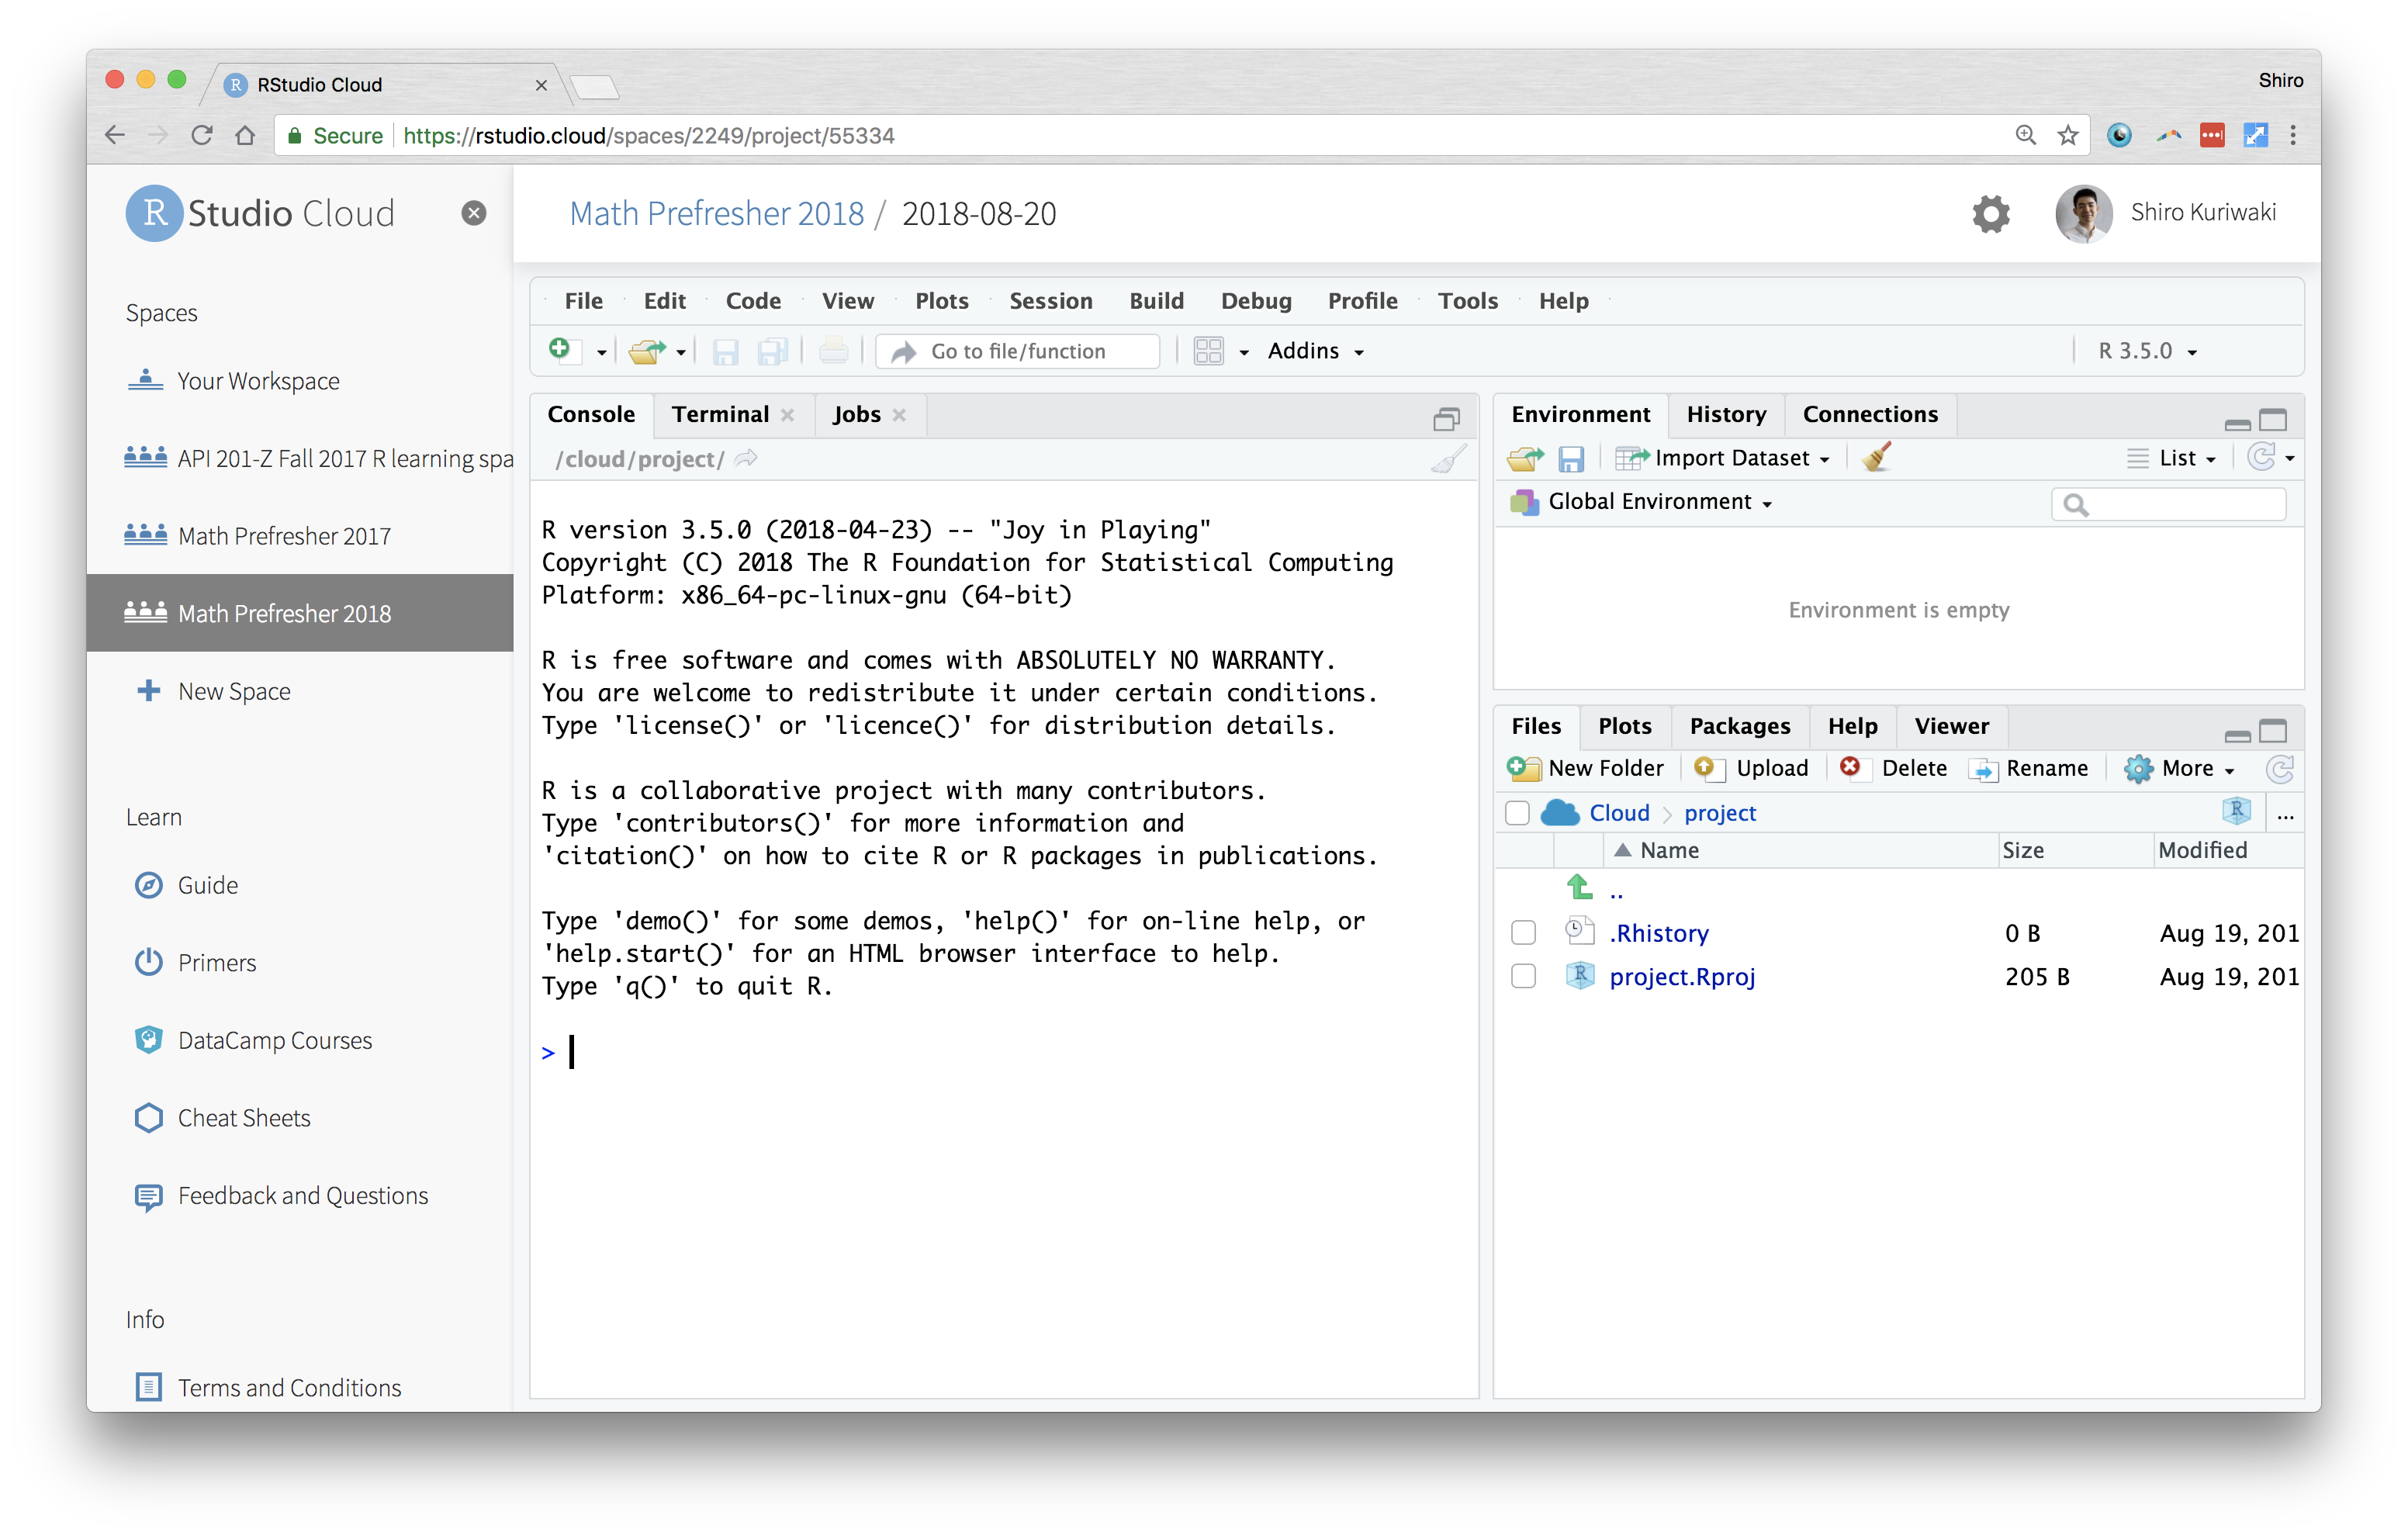
\includegraphics{images/11_1_rstudio-startup.png}
\caption{A Typical RStudio Window at Startup}
\end{figure}

\begin{enumerate}
\def\labelenumi{\arabic{enumi}.}
\setcounter{enumi}{2}
\item
  via the GUI, you the analyst needs to sends instructions, or \textbf{commands}, to the R application. The verb for this is ``run'' or ``execute'' the command. Computer programs ask users to provide instructions in very specific formats. While a English-speaking human can understand a sentence with a few typos in it by filling in the blanks, the same typo or misplaced character would halt a computer program. Each program has its own requirements for how commands should be typed; after all, each of these is its own language. We refer to the way a program needs its commands to be formatted as its \textbf{syntax}.
\item
  Theoretically, one could do all their work by typing in commands into the Console. But that would be a lot of work, because you'd have to give instructions each time you start your data analysis. Moreover, you'll have no record of what you did. That's why you need a \textbf{script}. This is a type of \textbf{code}. It can be referred to as a \textbf{source} because that is the source of your commands. Source is also used as a verb; ``source the script'' just means execute it. RStudio doesn't start out with a script, so you can make one from ``File \textgreater{} New'' or the New file icon.
\end{enumerate}

\begin{figure}
\centering
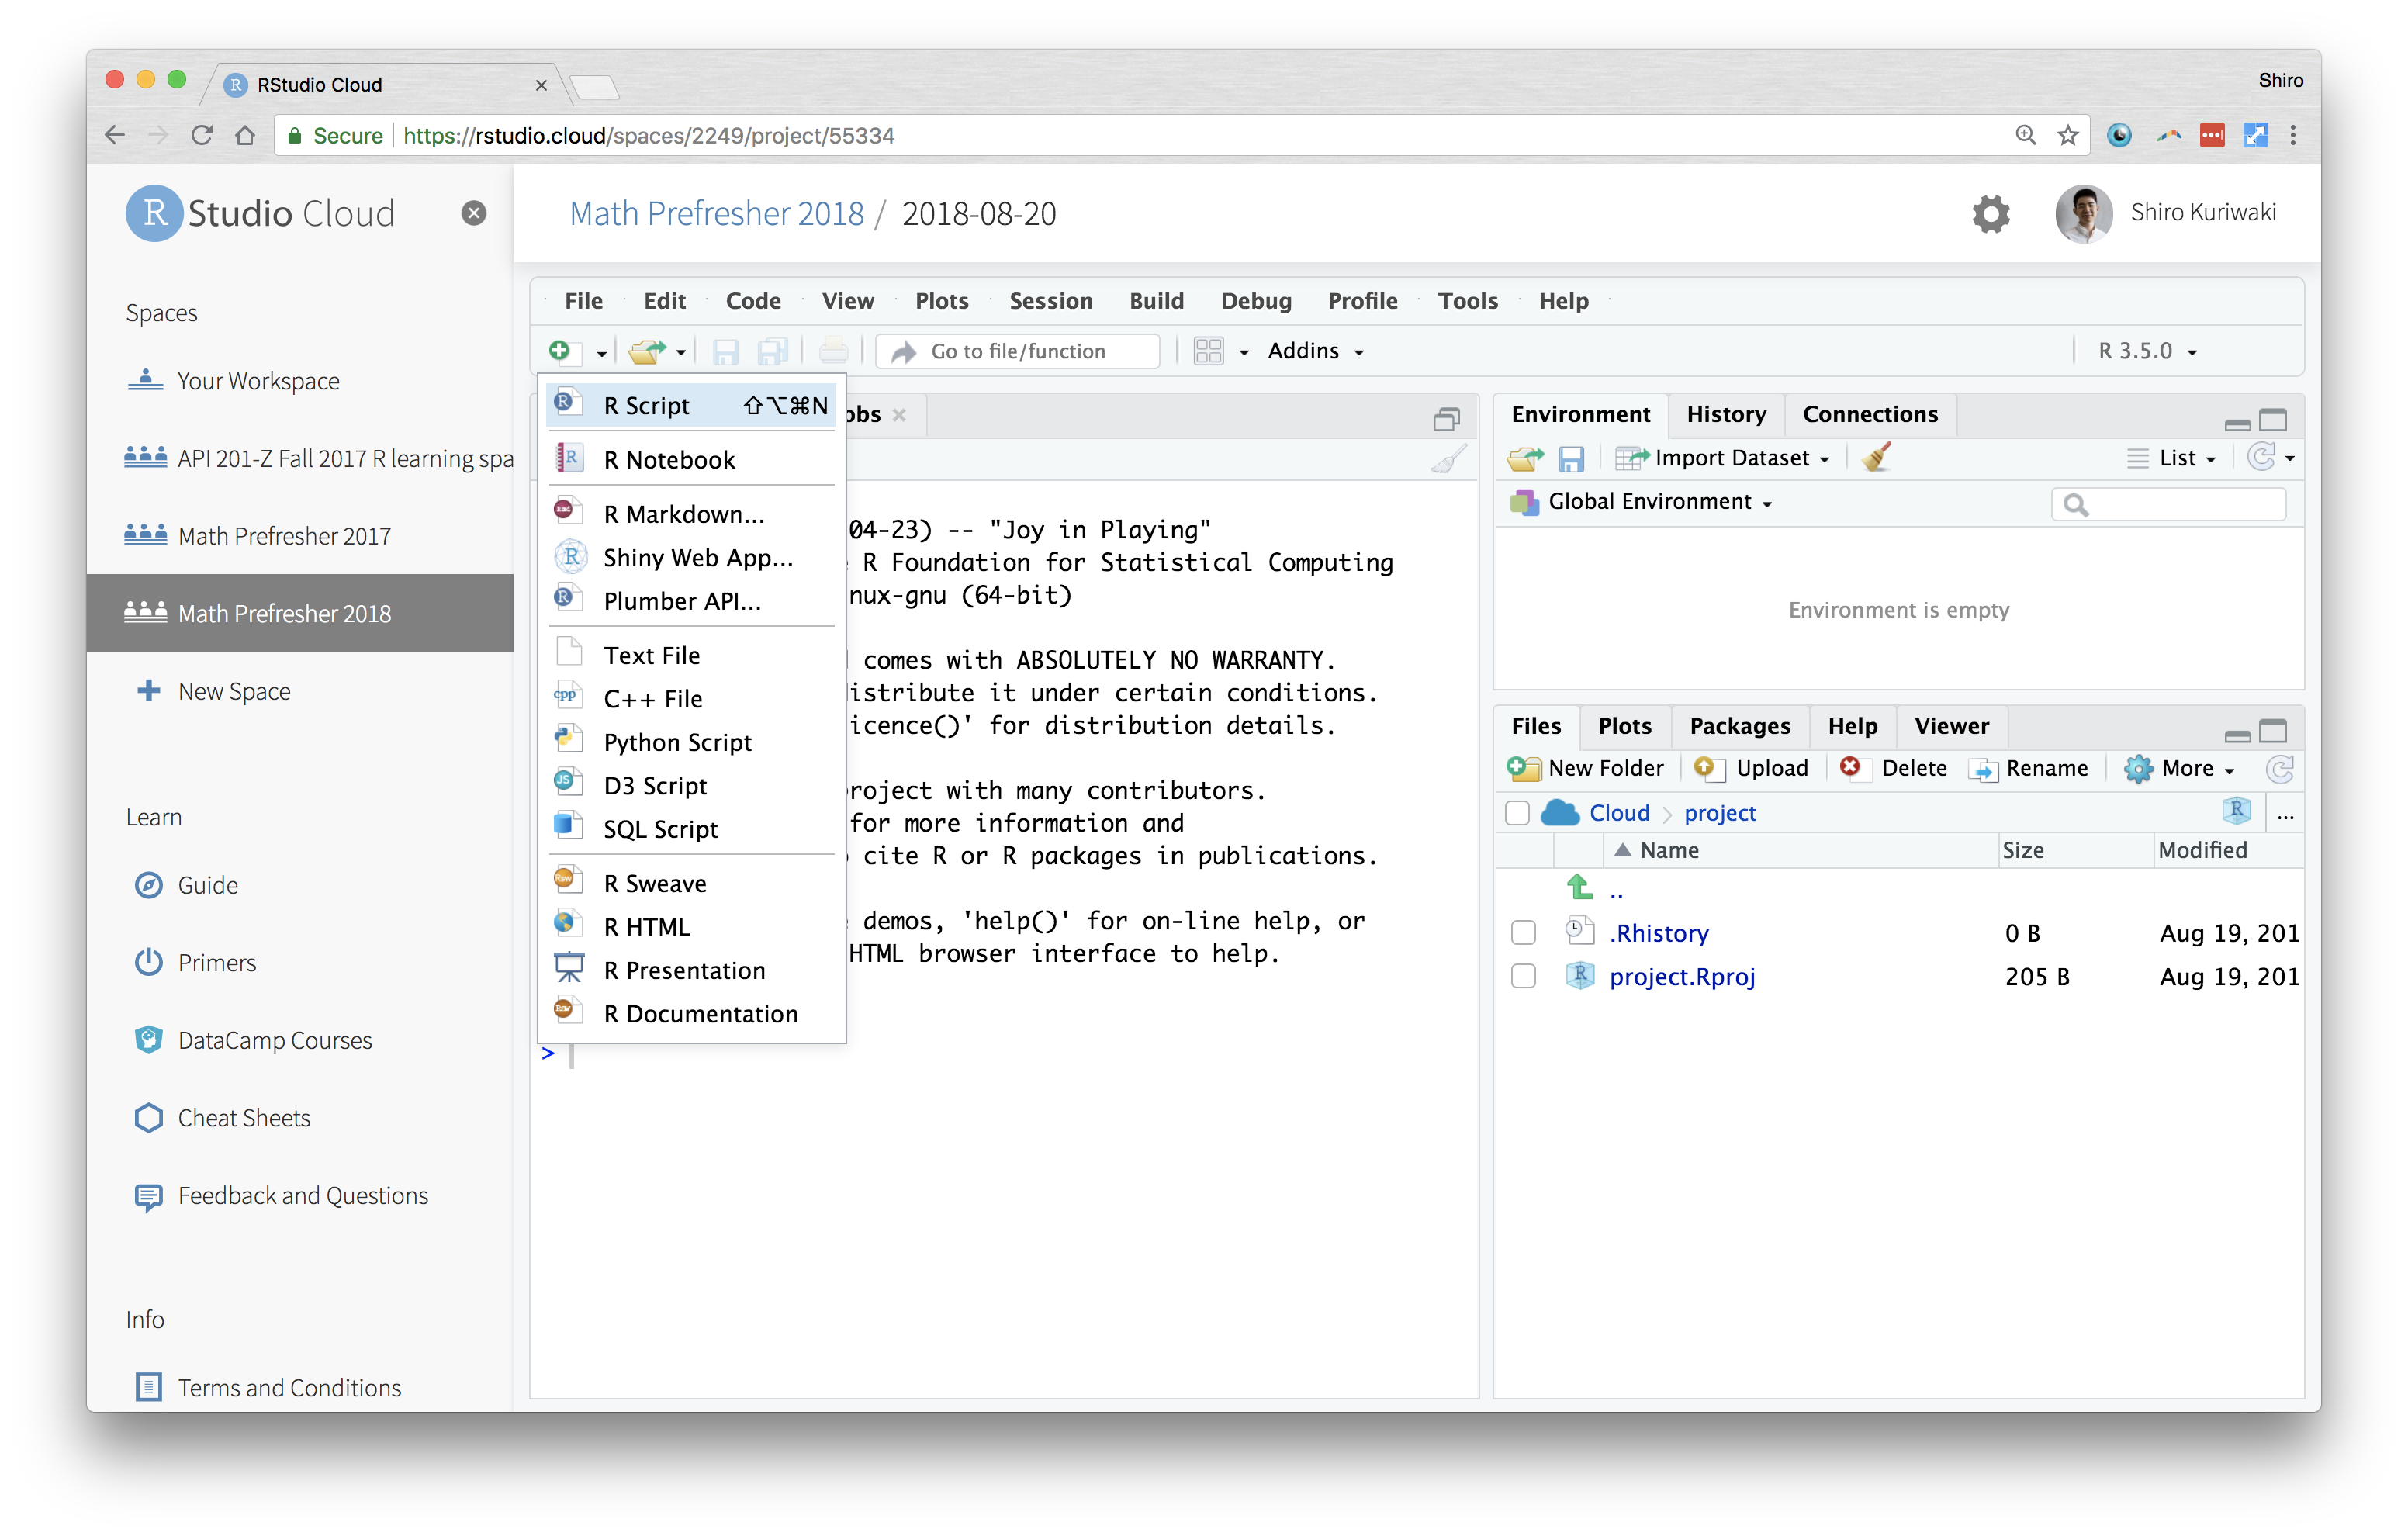
\includegraphics{images/11_2_rstudio-script.png}
\caption{Opening New Script (as opposed to the Console)}
\end{figure}

\begin{enumerate}
\def\labelenumi{\arabic{enumi}.}
\setcounter{enumi}{3}
\item
  You can also open scripts that are in folders in your computer. A script is a type of File. Find your Files in the bottom-right ``Files'' pane.

  To load a dataset, you need to specify where that file is. Computer files (data, documents, programs) are organized hiearchically, like a branching tree. Folders can contain files, and also other folders. The GUI toolbar makes this lineaer and hiearchical relationship apparent. When we turn to locate the file in our commands, we need another set of syntax. Importantly, denote the hierarchy of a folder by the \texttt{/} (slash) symbol. \texttt{data/input/2018-08} indicates the \texttt{2018-08} folder, which is included in the \texttt{input} folder, which is in turn included in the \texttt{data} folder.

  Files (but not folders) have ``file extensions'' which you are probably familiar with already: \texttt{.docx}, \texttt{.pdf}, and \texttt{.pdf}. The file extensions you will see in a stats or quantitative social science class are:

  \begin{itemize}
  \item
    \texttt{.pdf}: PDF, a convenient format to view documents and slides in, regardless of Mac/Windows.
  \item
    \texttt{.csv}: A comma separated values file
  \item
    \texttt{.xlsx}: Microsoft Excel file
  \item
    \texttt{.dta}: Stata data
  \item
    \texttt{.sav}: SPSS data
  \item
    \texttt{.R}: R code (script)
  \item
    \texttt{.Rmd}: Rmarkdown code (text + code)
  \item
    \texttt{.do}: Stata code (script)
  \end{itemize}
\end{enumerate}

\begin{figure}
\centering
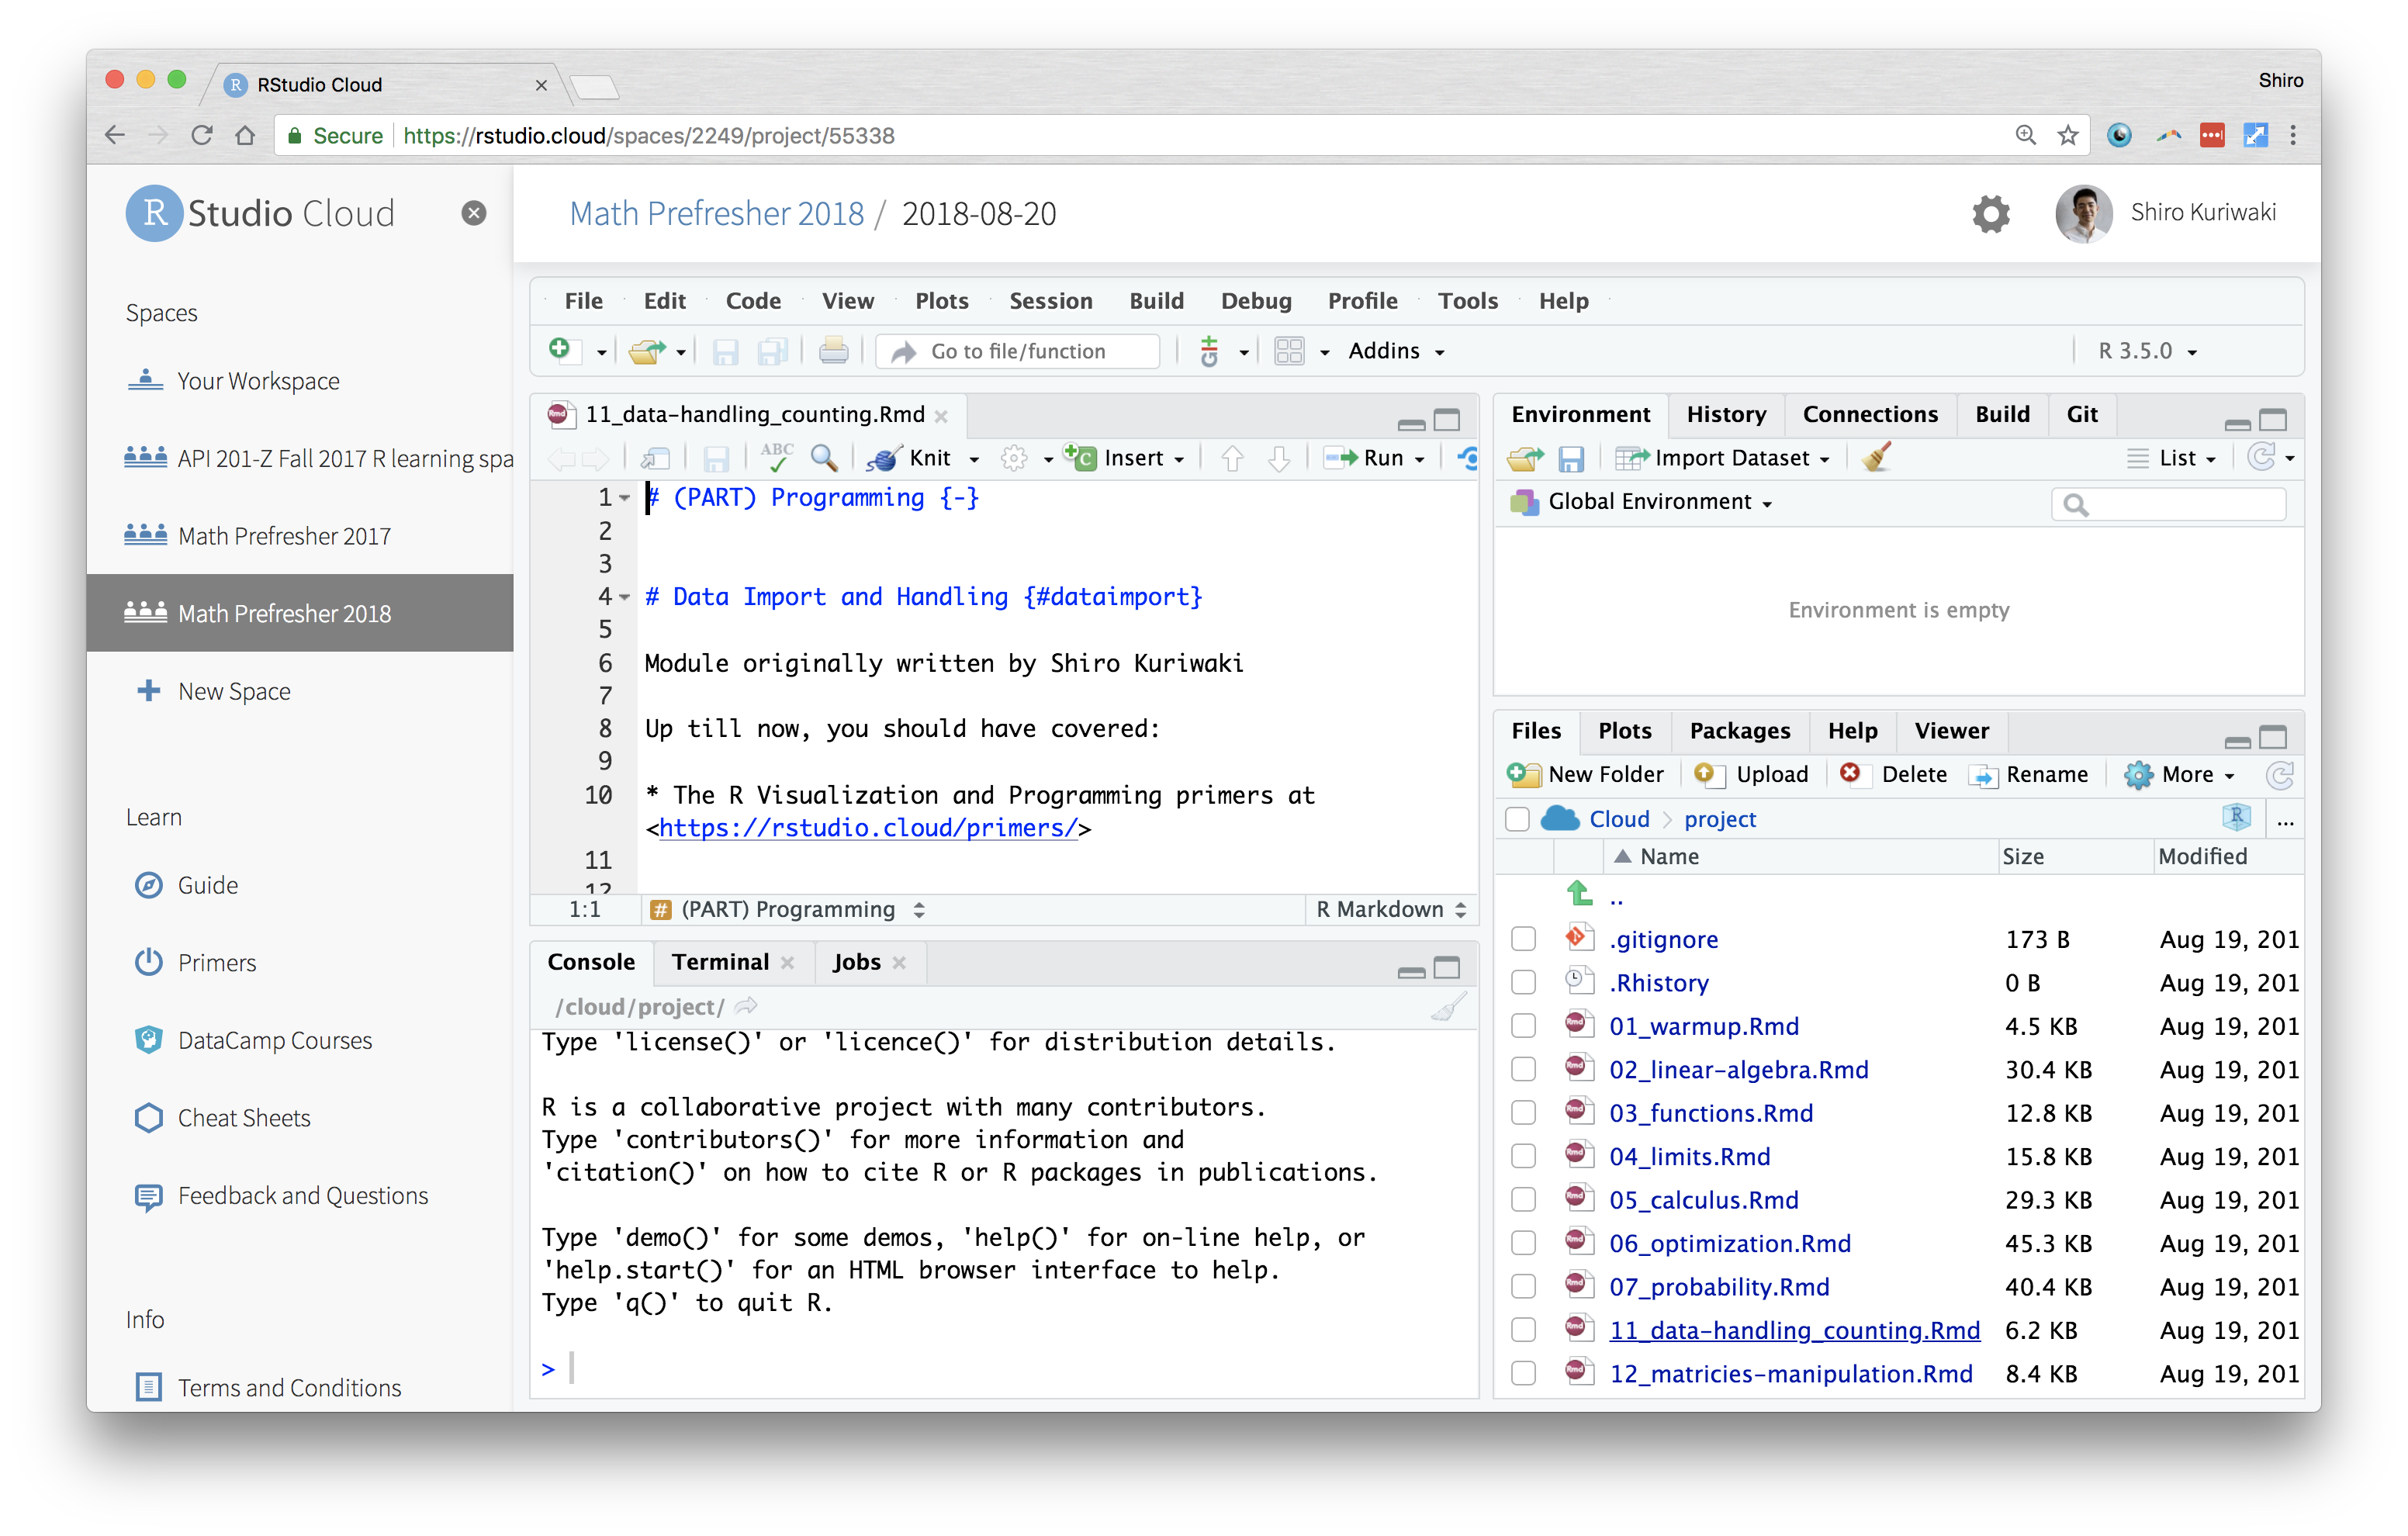
\includegraphics{images/11_3_rstudio-files.png}
\caption{Opening an Existing Script from Files}
\end{figure}

\begin{enumerate}
\def\labelenumi{\arabic{enumi}.}
\setcounter{enumi}{4}
\tightlist
\item
  In R, there are two main types of scripts. A classic \texttt{.R} file and a \texttt{.Rmd} file (for Rmarkdown). A .R file is just lines and lines of R code that is meant to be inserted right into the Console. A .Rmd tries to weave code and English together, to make it easier for users to create reports that interact with data and intersperse R code with explanation. For example, we built this book in Rmds.
\end{enumerate}

\begin{verbatim}
The Rmarkdown facilitates is the use of __code chunks__, which are used here. These start and end with three back-ticks. In the beginning, we can add options in curly braces (`{}`). Specifying `r` in the beginning tells to render it as R code. Options like `echo = TRUE` switch between showing the code that was executed or not; `eval = TRUE` switch between evaluating the code. More about Rmarkdown in Section \\ref{nonwysiwyg}. For example, this code chunk would evaluate `1 + 1` and show its output when compiled, but not display the code that was executed.
\end{verbatim}

\begin{figure}
\centering
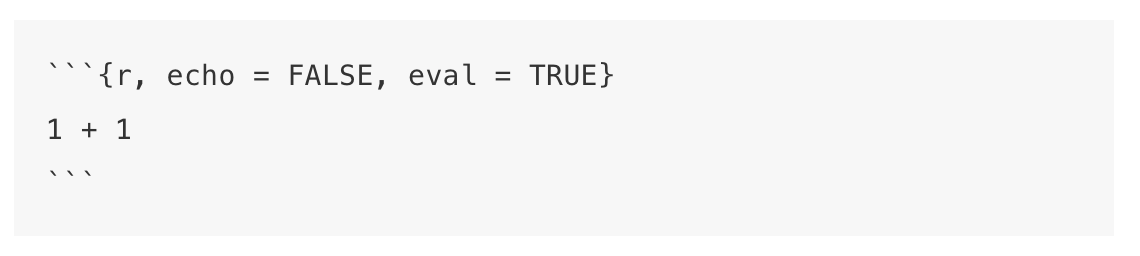
\includegraphics{images/11_4_codechunk.png}
\caption{A code chunk in Rmarkdown (before rendering)}
\end{figure}

\hypertarget{the-computer-and-you-giving-instructions}{%
\section{The Computer and You: Giving Instructions}\label{the-computer-and-you-giving-instructions}}

We'll do the Peanut Butter and Jelly Exercise in class as an introduction to programming for those who are new.\footnote{This Exercise is taken from Harvard's Introductory Undergraduate Class, CS50 (\url{https://www.youtube.com/watch?v=kcbT3hrEi9s}), and many other writeups.}

Assignment: Take 5 minutes to write down on a piece of paper, how to make a peanut butter and jelly sandwich. Be as concise and unambiguous as possible so that a robot (who doesn't know what a PBJ is) would understand. You can assume that there will be loaf of sliced bread, a jar of jelly, a jar of peanut butter, and a knife.

\hypertarget{base-r-vs.tidyverse}{%
\section{Base-R vs.~tidyverse}\label{base-r-vs.tidyverse}}

One last thing before we jump into data. Many things in R and other open source packages have competing standards. A lecture on a technique inevitably biases one standard over another. Right now among R users in this area, there are two families of functions: base-R and tidyverse. R instructors thus face a dilemma about which to teach primarily.\footnote{See for example this community discussion: \url{https://community.rstudio.com/t/base-r-and-the-tidyverse/2965/17}}

In this prefresher, we try our best to choose the one that is most useful to the modal task of social science researchers, and make use of the tidyverse functions in most applications. but feel free to suggest changes to us or to the booklet.

Although you do not need to choose one over the other, for beginners it is confusing what is a tidyverse function and what is not. Many of the tidyverse \emph{packages} are covered in this 2017 graphic below, and the cheat-sheets that other programmers have written: \url{https://www.rstudio.com/resources/cheatsheets/}

\begin{figure}
\centering
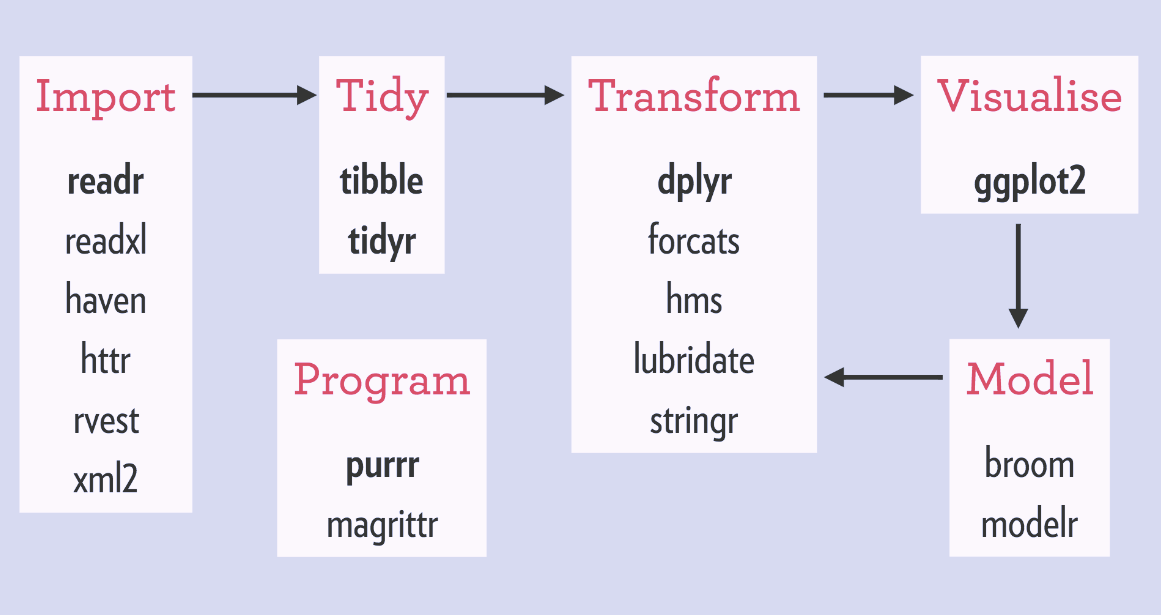
\includegraphics{images/tidyverse-packages.png}
\caption{Names of Packages in the tidyverse Family}
\end{figure}

The following side-by-side comparison of commands for a particular function compares some tidyverse and non-tidyverse functions (which we refer to loosely as base-R). This list is not meant to be comprehensive and more to give you a quick rule of thumb.

\hypertarget{dataframe-subsetting}{%
\subsection*{Dataframe subsetting}\label{dataframe-subsetting}}
\addcontentsline{toc}{subsection}{Dataframe subsetting}

\begin{longtable}[]{@{}lll@{}}
\toprule
\begin{minipage}[b]{0.29\columnwidth}\raggedright
In order to \ldots{}\strut
\end{minipage} & \begin{minipage}[b]{0.33\columnwidth}\raggedright
in tidyverse:\strut
\end{minipage} & \begin{minipage}[b]{0.30\columnwidth}\raggedright
in base-R:\strut
\end{minipage}\tabularnewline
\midrule
\endhead
\begin{minipage}[t]{0.29\columnwidth}\raggedright
Count each category\strut
\end{minipage} & \begin{minipage}[t]{0.33\columnwidth}\raggedright
\texttt{count(df,\ var)}\strut
\end{minipage} & \begin{minipage}[t]{0.30\columnwidth}\raggedright
\texttt{table(df\$var)}\strut
\end{minipage}\tabularnewline
\begin{minipage}[t]{0.29\columnwidth}\raggedright
Filter rows by condition\strut
\end{minipage} & \begin{minipage}[t]{0.33\columnwidth}\raggedright
\texttt{filter(df,\ var\ ==\ "Female")}\strut
\end{minipage} & \begin{minipage}[t]{0.30\columnwidth}\raggedright
\texttt{df{[}df\$var\ ==\ "Female",\ {]}} or \texttt{subset(df,\ var\ ==\ "Female")}\strut
\end{minipage}\tabularnewline
\begin{minipage}[t]{0.29\columnwidth}\raggedright
Extract columns\strut
\end{minipage} & \begin{minipage}[t]{0.33\columnwidth}\raggedright
\texttt{select(df,\ var1,\ var2)}\strut
\end{minipage} & \begin{minipage}[t]{0.30\columnwidth}\raggedright
\texttt{df{[},\ c("var1",\ "var2"){]}}\strut
\end{minipage}\tabularnewline
\begin{minipage}[t]{0.29\columnwidth}\raggedright
Extract a single column as a vector\strut
\end{minipage} & \begin{minipage}[t]{0.33\columnwidth}\raggedright
\texttt{pull(df,\ var)}\strut
\end{minipage} & \begin{minipage}[t]{0.30\columnwidth}\raggedright
\texttt{df{[}{[}"var"{]}{]}} or \texttt{df{[},\ "var"{]}}\strut
\end{minipage}\tabularnewline
\begin{minipage}[t]{0.29\columnwidth}\raggedright
Combine rows\strut
\end{minipage} & \begin{minipage}[t]{0.33\columnwidth}\raggedright
\texttt{bind\_rows()}\strut
\end{minipage} & \begin{minipage}[t]{0.30\columnwidth}\raggedright
\texttt{rbind()}\strut
\end{minipage}\tabularnewline
\begin{minipage}[t]{0.29\columnwidth}\raggedright
Combine columns\strut
\end{minipage} & \begin{minipage}[t]{0.33\columnwidth}\raggedright
\texttt{bind\_cols()}\strut
\end{minipage} & \begin{minipage}[t]{0.30\columnwidth}\raggedright
\texttt{cbind()}\strut
\end{minipage}\tabularnewline
\begin{minipage}[t]{0.29\columnwidth}\raggedright
Create a dataframe\strut
\end{minipage} & \begin{minipage}[t]{0.33\columnwidth}\raggedright
\texttt{tibble(x\ =\ vec1,\ y\ =\ vec2)}\strut
\end{minipage} & \begin{minipage}[t]{0.30\columnwidth}\raggedright
\texttt{data.frame(x\ =\ vec1,\ y\ =\ vec2)}\strut
\end{minipage}\tabularnewline
\begin{minipage}[t]{0.29\columnwidth}\raggedright
Turn a dataframe into a tidyverse dataframe\strut
\end{minipage} & \begin{minipage}[t]{0.33\columnwidth}\raggedright
\texttt{tbl\_df(df)}\strut
\end{minipage} & \begin{minipage}[t]{0.30\columnwidth}\raggedright
\strut
\end{minipage}\tabularnewline
\bottomrule
\end{longtable}

Remember that tidyverse applies to \emph{dataframes} only, not vectors. For subsetting vectors, use the base-R functions with the square brackets.

\hypertarget{read-data}{%
\subsection*{Read data}\label{read-data}}
\addcontentsline{toc}{subsection}{Read data}

Some non-tidyverse functions are not quite ``base-R'' but have similar relationships to tidyverse. For these, we recommend using the \emph{tidyverse} functions as a general rule due to their common format, simplicity, and scalability.

\begin{longtable}[]{@{}lll@{}}
\toprule
\begin{minipage}[b]{0.29\columnwidth}\raggedright
In order to \ldots{}\strut
\end{minipage} & \begin{minipage}[b]{0.33\columnwidth}\raggedright
in tidyverse:\strut
\end{minipage} & \begin{minipage}[b]{0.30\columnwidth}\raggedright
in base-R:\strut
\end{minipage}\tabularnewline
\midrule
\endhead
\begin{minipage}[t]{0.29\columnwidth}\raggedright
Read a Excel file\strut
\end{minipage} & \begin{minipage}[t]{0.33\columnwidth}\raggedright
\texttt{read\_excel()}\strut
\end{minipage} & \begin{minipage}[t]{0.30\columnwidth}\raggedright
\texttt{read.xlsx()}\strut
\end{minipage}\tabularnewline
\begin{minipage}[t]{0.29\columnwidth}\raggedright
Read a csv\strut
\end{minipage} & \begin{minipage}[t]{0.33\columnwidth}\raggedright
\texttt{read\_csv()}\strut
\end{minipage} & \begin{minipage}[t]{0.30\columnwidth}\raggedright
\texttt{read.csv()}\strut
\end{minipage}\tabularnewline
\begin{minipage}[t]{0.29\columnwidth}\raggedright
Read a Stata file\strut
\end{minipage} & \begin{minipage}[t]{0.33\columnwidth}\raggedright
\texttt{read\_dta()}\strut
\end{minipage} & \begin{minipage}[t]{0.30\columnwidth}\raggedright
\texttt{read.dta()}\strut
\end{minipage}\tabularnewline
\begin{minipage}[t]{0.29\columnwidth}\raggedright
Substitute strings\strut
\end{minipage} & \begin{minipage}[t]{0.33\columnwidth}\raggedright
\texttt{str\_replace()}\strut
\end{minipage} & \begin{minipage}[t]{0.30\columnwidth}\raggedright
\texttt{gsub()}\strut
\end{minipage}\tabularnewline
\begin{minipage}[t]{0.29\columnwidth}\raggedright
Return matching strings\strut
\end{minipage} & \begin{minipage}[t]{0.33\columnwidth}\raggedright
\texttt{str\_subset()}\strut
\end{minipage} & \begin{minipage}[t]{0.30\columnwidth}\raggedright
\texttt{grep(.,\ value\ =\ TRUE)}\strut
\end{minipage}\tabularnewline
\begin{minipage}[t]{0.29\columnwidth}\raggedright
Merge \texttt{data1} and \texttt{data2} on variables \texttt{x1} and \texttt{x2}\strut
\end{minipage} & \begin{minipage}[t]{0.33\columnwidth}\raggedright
\texttt{left\_join(data1,\ data2,\ by\ =\ c("x1",\ "x2"))}\strut
\end{minipage} & \begin{minipage}[t]{0.30\columnwidth}\raggedright
\texttt{merge(data1,\ data2,\ by.x\ =\ "x1",\ by.y\ =\ "x2",\ all.x\ =\ TRUE)}\strut
\end{minipage}\tabularnewline
\bottomrule
\end{longtable}

\hypertarget{visualization}{%
\subsection*{Visualization}\label{visualization}}
\addcontentsline{toc}{subsection}{Visualization}

Plotting by ggplot2 (from your tutorials) is also a tidyverse family.

\begin{longtable}[]{@{}lll@{}}
\toprule
\begin{minipage}[b]{0.29\columnwidth}\raggedright
In order to \ldots{}\strut
\end{minipage} & \begin{minipage}[b]{0.33\columnwidth}\raggedright
in tidyverse:\strut
\end{minipage} & \begin{minipage}[b]{0.30\columnwidth}\raggedright
in base-R:\strut
\end{minipage}\tabularnewline
\midrule
\endhead
\begin{minipage}[t]{0.29\columnwidth}\raggedright
Make a scatter plot\strut
\end{minipage} & \begin{minipage}[t]{0.33\columnwidth}\raggedright
\texttt{ggplot(data,\ aes(x,\ y))\ +\ geom\_point()}\strut
\end{minipage} & \begin{minipage}[t]{0.30\columnwidth}\raggedright
\texttt{plot(data\$x,\ data\$y)}\strut
\end{minipage}\tabularnewline
\begin{minipage}[t]{0.29\columnwidth}\raggedright
Make a line plot\strut
\end{minipage} & \begin{minipage}[t]{0.33\columnwidth}\raggedright
\texttt{ggplot(data,\ aes(x,\ y))\ +\ geom\_line()}\strut
\end{minipage} & \begin{minipage}[t]{0.30\columnwidth}\raggedright
\texttt{plot(data\$x,\ data\$y,\ type\ =\ "l")}\strut
\end{minipage}\tabularnewline
\begin{minipage}[t]{0.29\columnwidth}\raggedright
Make a histogram\strut
\end{minipage} & \begin{minipage}[t]{0.33\columnwidth}\raggedright
\texttt{ggplot(data,\ aes(x,\ y))\ +\ geom\_histogram()}\strut
\end{minipage} & \begin{minipage}[t]{0.30\columnwidth}\raggedright
\texttt{hist(data\$x,\ data\$y)}\strut
\end{minipage}\tabularnewline
\begin{minipage}[t]{0.29\columnwidth}\raggedright
Make a barplot\strut
\end{minipage} & \begin{minipage}[t]{0.33\columnwidth}\raggedright
See Section \ref{dataviz}\strut
\end{minipage} & \begin{minipage}[t]{0.30\columnwidth}\raggedright
See Section \ref{dataviz}\strut
\end{minipage}\tabularnewline
\bottomrule
\end{longtable}

\hypertarget{a-is-for-athens}{%
\section{A is for Athens}\label{a-is-for-athens}}

For our first dataset, let's try reading in a dataset on the Ancient Greek world. Political Theorists and Political Historians study the domestic systems, international wars, cultures and writing of this era to understand the first instance of democracy, the rise and overturning of tyranny, and the legacies of political institutions.

This POLIS dataset was generously provided by Professor Josiah Ober of Stanford University. This dataset includes information on city states in the Ancient Greek world, parts of it collected by careful work by historians and archaeologists. It is part of his recent books on Greece (Ober 2015), ``The Rise and Fall of Classical Greece''\footnote{\href{https://press.princeton.edu/titles/10423.html}{Ober, Josiah (2015). \emph{The Rise and Fall of Classical Greece}. Princeton University Press.}} and Institutions in Ancient Athens (Ober 2010) , ``Democracy and Knowledge: Innovation and Learning in Classical Athens.''\footnote{\href{https://press.princeton.edu/titles/8742.html}{Ober, Josiah (2010). \emph{Democracy and Knowledge: Innovation and Learning in Classical Athens}. Princeton University Press.}}

\hypertarget{locating-the-data}{%
\subsection{Locating the Data}\label{locating-the-data}}

What files do we have in the \texttt{input} folder?

\begin{verbatim}
## input/Nunn_Wantchekon_AER_2011.dta
## input/Nunn_Wantchekon_sample.dta
## input/acs2015_1percent.csv
## input/complete_greek_data 5 DISTRIBUTION 2018.xlsx
## input/gapminder_wide.Rds
## input/gapminder_wide.tab
## input/german_credit.sav
## input/justices_court-median.csv
## input/sample_mid.csv
## input/sample_polity.csv
## input/upshot-siena-polls.csv
## input/usc2010_001percent.csv
## input/usc2010_1percent.Rds
\end{verbatim}

A typical file format is Microsoft Excel. Although this is not usually the best format for R because of its highly formatted structure as opposed to plain text (more on this in Section \ref@(sec:wysiwyg)), recent packages have made this fairly easy.

For the first time using an outside package, you first need to install it.

\begin{Shaded}
\begin{Highlighting}[]
\KeywordTok{install.packages}\NormalTok{(}\StringTok{"readxl"}\NormalTok{)}
\end{Highlighting}
\end{Shaded}

After that, you don't need to install it again. But you \textbf{do} need to load it each time.

\begin{Shaded}
\begin{Highlighting}[]
\KeywordTok{library}\NormalTok{(readxl)}
\end{Highlighting}
\end{Shaded}

The package \texttt{readxl} has a website: \url{https://readxl.tidyverse.org/}. Other packages are not as user-friendly, but they have a help page with a table of contents of all their functions.

\begin{Shaded}
\begin{Highlighting}[]
\KeywordTok{help}\NormalTok{(}\DataTypeTok{package =}\NormalTok{ readxl)}
\end{Highlighting}
\end{Shaded}

\hypertarget{reading-in-data}{%
\subsection{Reading in Data}\label{reading-in-data}}

From the help page, we see that \texttt{read\_excel()} is the function that we want to use. Look at the help page. How do you read a help page?

Let's try it.

\begin{Shaded}
\begin{Highlighting}[]
\NormalTok{ober <-}\StringTok{ }\KeywordTok{read_excel}\NormalTok{(}\StringTok{"input/complete_greek_data 5 DISTRIBUTION 2018.xlsx"}\NormalTok{)}
\end{Highlighting}
\end{Shaded}

\begin{verbatim}
## New names:
## * `` -> ...35
\end{verbatim}

Review: what does the \texttt{/} mean? Why do we need the \texttt{input} term first? Does the argument need to be in quotes?

\hypertarget{inspecting}{%
\subsection{Inspecting}\label{inspecting}}

For almost any dataset, you usually want to do a couple of standard checks first to understand what you loaded.

\begin{Shaded}
\begin{Highlighting}[]
\NormalTok{ober}
\end{Highlighting}
\end{Shaded}

\begin{verbatim}
## # A tibble: 1,035 x 35
##    polis_number Name  Polisity Hellenicity  Fame `In/out`  Size
##           <dbl> <chr>    <dbl>       <dbl> <dbl>    <dbl> <dbl>
##  1            1 Alal~        1           1  1.12        1     3
##  2            2 Empo~        1           2  2.12        2     2
##  3            3 Mass~        1           1  4           2     2
##  4            4 Rhode        2           1  0.87        3     0
##  5            5 Abak~        2           2  1           2     0
##  6            6 Adra~        2           1  1           3     0
##  7            7 Agyr~        2           1  1.25        2     0
##  8            8 Aitna        1           1  3.25        1     4
##  9            9 Akra~        1           1  6.37        4     5
## 10           10 Akrai        3           1  1.25        2     0
## # ... with 1,025 more rows, and 28 more variables: `Silver-1st` <dbl>,
## #   `Bronze 1st` <dbl>, Grid <dbl>, Colonies <dbl>, Victors <dbl>,
## #   Proxenoi <dbl>, Walls <dbl>, `Delian L` <dbl>, Koinon <dbl>,
## #   Regime <dbl>, `Region #` <dbl>, `Region name` <chr>, Latitude <dbl>,
## #   Longitude <dbl>, Source <chr>, `Elevation m` <dbl>, `Pleiades
## #   Control` <chr>, `Hanson Appearance` <dbl>, `Hanson Name` <chr>,
## #   `Hanson #` <dbl>, `Occupied From (Hanson)` <dbl>, `Size (ha.)` <chr>,
## #   `Hanson Longitude` <dbl>, `Hanson Latitude` <dbl>, `Lat O-H` <dbl>,
## #   `Long O-H` <dbl>, `Absolute Lat+Long O-H` <dbl>, ...35 <chr>
\end{verbatim}

\begin{Shaded}
\begin{Highlighting}[]
\KeywordTok{dim}\NormalTok{(ober)}
\end{Highlighting}
\end{Shaded}

\begin{verbatim}
## [1] 1035   35
\end{verbatim}

From your tutorials, you also know how to do graphics! Graphics are useful for grasping your data, but we will cover them more deeply in Chapter \ref{dataviz}.

\begin{Shaded}
\begin{Highlighting}[]
\KeywordTok{ggplot}\NormalTok{(ober, }\KeywordTok{aes}\NormalTok{(}\DataTypeTok{x =}\NormalTok{ Fame)) }\OperatorTok{+}\StringTok{ }\KeywordTok{geom_histogram}\NormalTok{()}
\end{Highlighting}
\end{Shaded}

\begin{verbatim}
## `stat_bin()` using `bins = 30`. Pick better value with `binwidth`.
\end{verbatim}

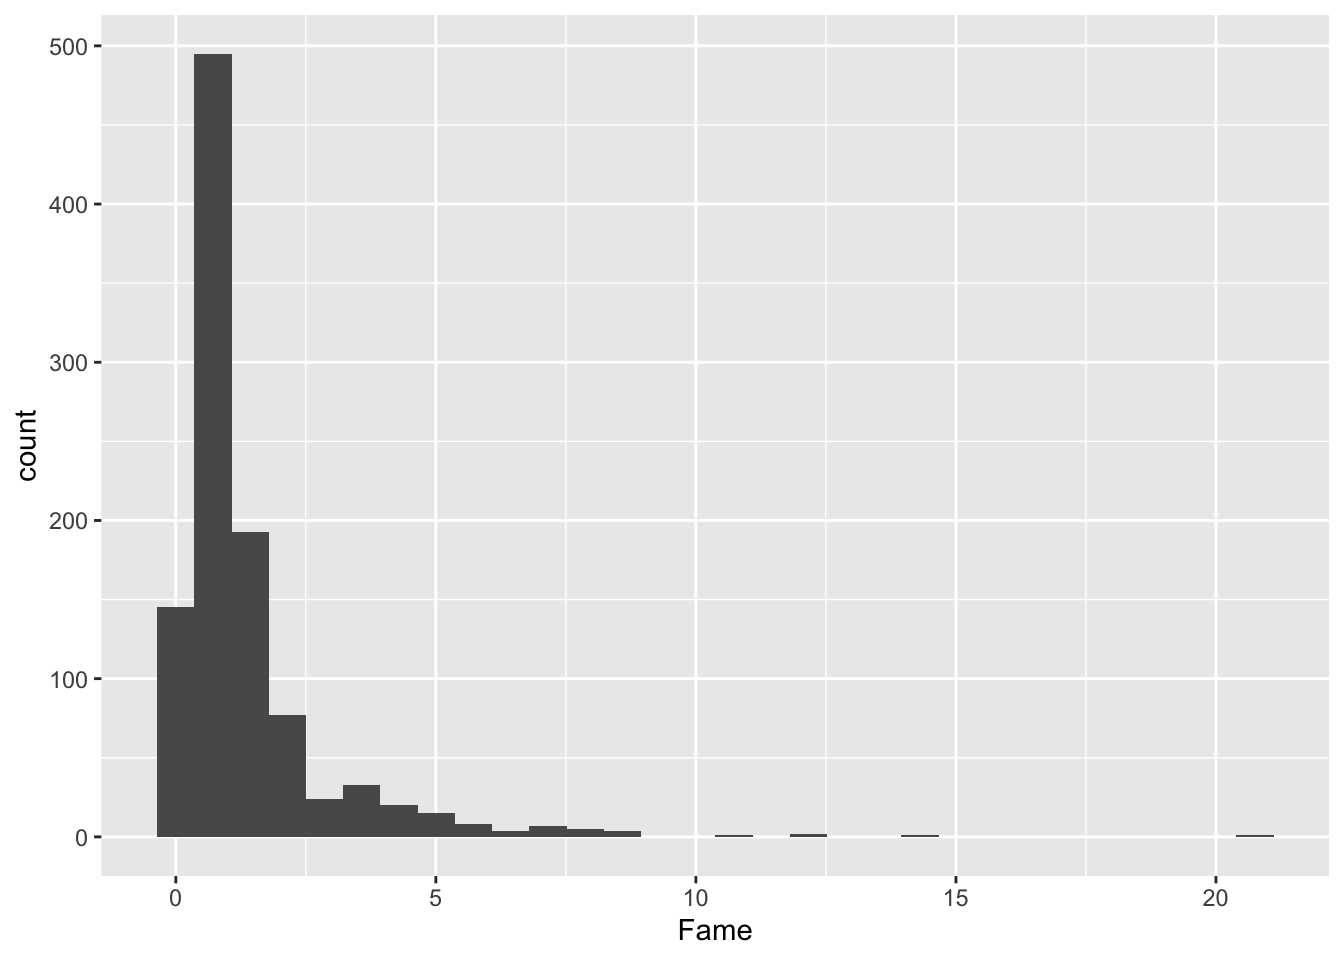
\includegraphics{prefresher_files/figure-latex/unnamed-chunk-103-1.pdf}

What about the distribution of fame by regime?

\begin{Shaded}
\begin{Highlighting}[]
\KeywordTok{ggplot}\NormalTok{(ober, }\KeywordTok{aes}\NormalTok{(}\DataTypeTok{y =}\NormalTok{ Fame, }\DataTypeTok{x =} \KeywordTok{factor}\NormalTok{(Regime), }\DataTypeTok{group =} \KeywordTok{factor}\NormalTok{(Regime))) }\OperatorTok{+}
\StringTok{  }\KeywordTok{geom_boxplot}\NormalTok{()}
\end{Highlighting}
\end{Shaded}

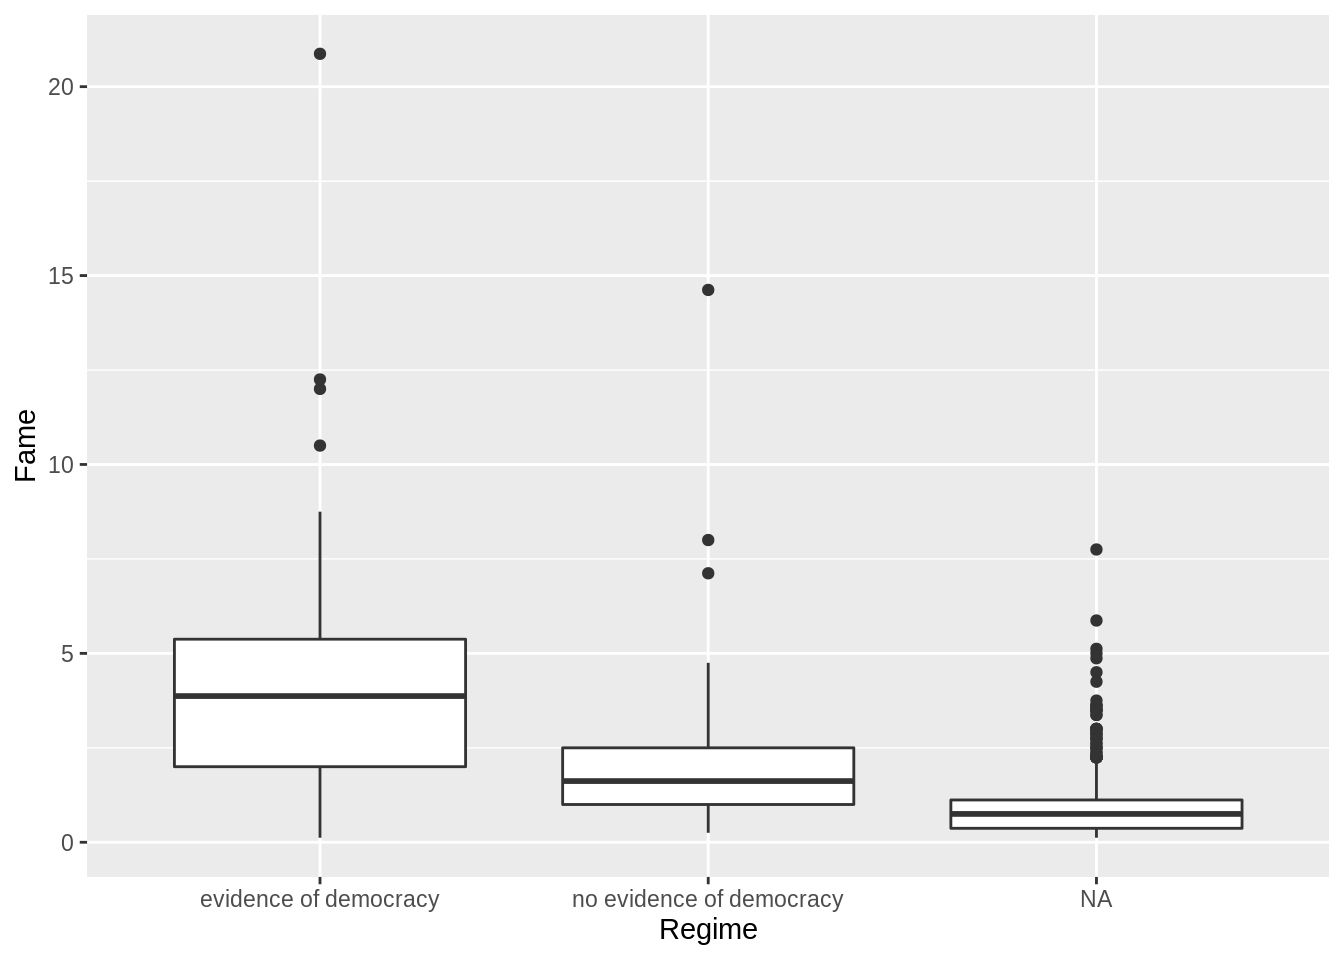
\includegraphics{prefresher_files/figure-latex/unnamed-chunk-104-1.pdf}

What do the 1's, 2's, and 3's stand for?

\hypertarget{finding-observations}{%
\subsection{Finding observations}\label{finding-observations}}

These \texttt{tidyverse} commands from the \texttt{dplyr} package are newer and not built-in, but they are one of the increasingly more popular ways to wrangle data.

\begin{itemize}
\tightlist
\item
  80 percent of your data wrangling needs might be doable with these basic \texttt{dplyr} functions: \texttt{select}, \texttt{mutate}, \texttt{group\_by}, \texttt{summarize}, and \texttt{arrange}.
\item
  These verbs roughly correspond to the same commands in SQL, another important language in data science.
\item
  The \texttt{\%\textgreater{}\%} symbol is a pipe. It takes the thing on the left side and pipes it down to the function on the right side. We could have done \texttt{count(cen10,\ race)} as \texttt{cen10\ \%\textgreater{}\%\ count(race)}. That means take \texttt{cen10} and pass it on to the function \texttt{count}, which will count observations by race and return a collapsed dataset with the categories in its own variable and their respective counts in \texttt{n}.
\end{itemize}

\hypertarget{extra-a-sneak-peak-at-obers-data}{%
\subsection{Extra: A sneak peak at Ober's data}\label{extra-a-sneak-peak-at-obers-data}}

Although this is a bit beyond our current stage, it's hard to resist the temptation to see what you can do with data like this. For example, you can map it.\footnote{In mid-2018, changes in Google's services made it no longer possible to render maps on the fly. Therefore, no map is currently rendered. Instead, you now need to register with Google. See the \href{https://github.com/dkahle/ggmap/blob/e55c0b22b0d16a010b4b45dd2fce800ff0ef19b8/NEWS\#L6-L12}{change} to the pacakge ggmap }

Using the \texttt{ggmap} package

\begin{Shaded}
\begin{Highlighting}[]
\KeywordTok{library}\NormalTok{(ggmap)}
\end{Highlighting}
\end{Shaded}

First get a map of the Greek world.

\begin{Shaded}
\begin{Highlighting}[]
\NormalTok{greece <-}\StringTok{ }\KeywordTok{get_map}\NormalTok{(}\DataTypeTok{location =} \KeywordTok{c}\NormalTok{(}\DataTypeTok{lon =} \FloatTok{22.6382849}\NormalTok{, }\DataTypeTok{lat =} \FloatTok{39.543287}\NormalTok{),}
                  \DataTypeTok{zoom =} \DecValTok{5}\NormalTok{, }
                  \DataTypeTok{source =} \StringTok{"stamen"}\NormalTok{,}
                  \DataTypeTok{maptype =} \StringTok{"toner"}\NormalTok{)}
\KeywordTok{ggmap}\NormalTok{(greece)}
\end{Highlighting}
\end{Shaded}

I chose the specifications for arguments \texttt{zoom} and \texttt{maptype} by looking at the webpage and Googling some examples/

Ober's data has the latitude and longitude of each polis. Because the map of Greece has the same coordinates, we can add the polei on the same map.

\begin{Shaded}
\begin{Highlighting}[]
\NormalTok{gg_ober <-}\StringTok{ }\KeywordTok{ggmap}\NormalTok{(greece) }\OperatorTok{+}
\StringTok{  }\KeywordTok{geom_point}\NormalTok{(}\DataTypeTok{data =}\NormalTok{ ober, }
             \KeywordTok{aes}\NormalTok{(}\DataTypeTok{y =}\NormalTok{ Latitude, }\DataTypeTok{x =}\NormalTok{ Longitude), }
             \DataTypeTok{size =} \FloatTok{0.5}\NormalTok{,}
             \DataTypeTok{alpha =} \FloatTok{0.5}\NormalTok{,}
             \DataTypeTok{color =} \StringTok{"gray"}\NormalTok{)}
\NormalTok{gg_ober}
\end{Highlighting}
\end{Shaded}

We can also color the points by another variable, like Fame.

\begin{Shaded}
\begin{Highlighting}[]
\NormalTok{gg_ober_fame <-}\StringTok{ }\KeywordTok{ggmap}\NormalTok{(greece) }\OperatorTok{+}
\StringTok{  }\KeywordTok{geom_point}\NormalTok{(}\DataTypeTok{data =}\NormalTok{ ober, }
             \KeywordTok{aes}\NormalTok{(}\DataTypeTok{y =}\NormalTok{ Latitude, }\DataTypeTok{x =}\NormalTok{ Longitude, }\DataTypeTok{color =}\NormalTok{ Fame)) }\OperatorTok{+}
\StringTok{  }\KeywordTok{scale_color_gradient}\NormalTok{(}\DataTypeTok{low =} \StringTok{"white"}\NormalTok{, }\DataTypeTok{high =} \StringTok{"indianred"}\NormalTok{)}
\NormalTok{gg_ober_fame}
\end{Highlighting}
\end{Shaded}

\hypertarget{exercises}{%
\section*{Exercises}\label{exercises}}
\addcontentsline{toc}{section}{Exercises}

\hypertarget{section}{%
\subsection*{1}\label{section}}
\addcontentsline{toc}{subsection}{1}

What is the Fame value of Delphoi?

\begin{Shaded}
\begin{Highlighting}[]
\CommentTok{# Enter here}
\end{Highlighting}
\end{Shaded}

\hypertarget{section-1}{%
\subsection*{2}\label{section-1}}
\addcontentsline{toc}{subsection}{2}

Find the polis with the top 10 Fame values.

\begin{Shaded}
\begin{Highlighting}[]
\CommentTok{# Enter here}
\end{Highlighting}
\end{Shaded}

\hypertarget{section-2}{%
\subsection*{3}\label{section-2}}
\addcontentsline{toc}{subsection}{3}

Make a scatterplot with the number of colonies on the x-axis and Fame on the y-axis.

\begin{Shaded}
\begin{Highlighting}[]
\CommentTok{# Enter here}
\end{Highlighting}
\end{Shaded}

\hypertarget{section-3}{%
\subsection*{4}\label{section-3}}
\addcontentsline{toc}{subsection}{4}

Find the correct function to read the following datasets (available in your rstudio.cloud session) into your R window.

\begin{itemize}
\tightlist
\item
  \texttt{input/acs2015\_1percent.csv}: A one percent sample of the American Community Survey
\item
  \texttt{input/gapminder\_wide.tab}: Country-level wealth and health from Gapminder\footnote{Formatted and taken from \url{https://doi.org/10.7910/DVN/GJQNEQ}}
\item
  \texttt{input/gapminder\_wide.Rds}: A Rds version of the Gapminder (What is a Rds file? What's the difference?)
\item
  \texttt{input/Nunn\_Wantchekon\_sample.dta}: A sample from the Afrobarometer survey (which we'll explore tomorrow). \texttt{.dta} is a Stata format.
\item
  \texttt{input/german\_credit.sav}: A hypothetical dataset on consumer credit. \texttt{.sav} is a SPSS format.
\end{itemize}

Our Recommendations: Look at the packages \texttt{haven} and \texttt{readr}

\begin{Shaded}
\begin{Highlighting}[]
\CommentTok{# Enter here, perhaps making a chunk for each file.}
\end{Highlighting}
\end{Shaded}

\hypertarget{section-4}{%
\subsection*{5}\label{section-4}}
\addcontentsline{toc}{subsection}{5}

Read Ober's codebook and find a variable that you think is interesting. Check the distribution of that variable in your data, get a couple of statistics, and summarize it in English.

\begin{Shaded}
\begin{Highlighting}[]
\CommentTok{# Enter here}
\end{Highlighting}
\end{Shaded}

\hypertarget{section-5}{%
\subsection*{6}\label{section-5}}
\addcontentsline{toc}{subsection}{6}

This is day 1 and we covered a lot of material. Some of you might have found this completely new; others not so. Please click through this survey before you leave so we can adjust accordingly on the next few days.

\url{https://harvard.az1.qualtrics.com/jfe/form/SV_8As7Y7C83iBiQzH}

\hypertarget{rmatrices}{%
\chapter[Manipulating Vectors and Matrices]{\texorpdfstring{Manipulating Vectors and Matrices\footnote{Module originally written by Shiro Kuriwaki and Yon Soo Park}}{Manipulating Vectors and Matrices}}\label{rmatrices}}

\hypertarget{where-are-we-where-are-we-headed-1}{%
\subsection*{Where are we? Where are we headed?}\label{where-are-we-where-are-we-headed-1}}
\addcontentsline{toc}{subsection}{Where are we? Where are we headed?}

Up till now, you should have covered:

\begin{itemize}
\tightlist
\item
  R basic programming
\item
  Data Import
\item
  Statistical Summaries.
\end{itemize}

Today we'll cover

\begin{itemize}
\tightlist
\item
  Matrices \& Dataframes in R
\item
  Manipulating variables
\item
  And other \texttt{R} tips
\end{itemize}

\hypertarget{basics---matrices}{%
\section{Basics - Matrices}\label{basics---matrices}}

Let's take a look at Matrices in the context of R

\begin{Shaded}
\begin{Highlighting}[]
\NormalTok{cen10 <-}\StringTok{ }\KeywordTok{read_csv}\NormalTok{(}\StringTok{"input/usc2010_001percent.csv"}\NormalTok{)}
\KeywordTok{head}\NormalTok{(cen10)}
\end{Highlighting}
\end{Shaded}

\begin{verbatim}
## # A tibble: 6 x 13
##    year serial pernum region state countyfips city  cpuma0010 sex     age
##   <dbl>  <dbl>  <dbl> <chr>  <chr>      <dbl> <chr>     <dbl> <chr> <dbl>
## 1  2010 8.80e6      4 Middl~ New ~          0 Not ~       636 Fema~     8
## 2  2010 9.80e6      1 East ~ Ohio         103 Not ~       802 Male     24
## 3  2010 8.69e6      1 Mount~ Neva~          3 Not ~       582 Male     37
## 4  2010 6.35e6      3 East ~ Mich~          0 Not ~       476 Fema~    12
## 5  2010 6.15e6      2 South~ Mary~         33 Not ~       449 Fema~    18
## 6  2010 8.10e6      1 New E~ New ~          0 Not ~       586 Male     50
## # ... with 3 more variables: race <chr>, hhtype <chr>, relate <chr>
\end{verbatim}

What is the dimension of this dataframe? What does the number of rows represent? What does the number of columns represent?

\begin{Shaded}
\begin{Highlighting}[]
\KeywordTok{dim}\NormalTok{(cen10)}
\end{Highlighting}
\end{Shaded}

\begin{verbatim}
## [1] 30871    13
\end{verbatim}

\begin{Shaded}
\begin{Highlighting}[]
\KeywordTok{nrow}\NormalTok{(cen10)}
\end{Highlighting}
\end{Shaded}

\begin{verbatim}
## [1] 30871
\end{verbatim}

\begin{Shaded}
\begin{Highlighting}[]
\KeywordTok{ncol}\NormalTok{(cen10)}
\end{Highlighting}
\end{Shaded}

\begin{verbatim}
## [1] 13
\end{verbatim}

What variables does this dataset hold? What kind of information does it have?

\begin{Shaded}
\begin{Highlighting}[]
\KeywordTok{colnames}\NormalTok{(cen10)}
\end{Highlighting}
\end{Shaded}

\begin{verbatim}
##  [1] "year"       "serial"     "pernum"     "region"     "state"     
##  [6] "countyfips" "city"       "cpuma0010"  "sex"        "age"       
## [11] "race"       "hhtype"     "relate"
\end{verbatim}

We can access column vectors, or vectors that contain values of variables by using the \$ sign

\begin{Shaded}
\begin{Highlighting}[]
\KeywordTok{head}\NormalTok{(cen10}\OperatorTok{$}\NormalTok{state)}
\end{Highlighting}
\end{Shaded}

\begin{verbatim}
## [1] "New York"      "Ohio"          "Nevada"        "Michigan"     
## [5] "Maryland"      "New Hampshire"
\end{verbatim}

\begin{Shaded}
\begin{Highlighting}[]
\KeywordTok{head}\NormalTok{(cen10}\OperatorTok{$}\NormalTok{city)}
\end{Highlighting}
\end{Shaded}

\begin{verbatim}
## [1] "Not in identifiable city (or size group)"
## [2] "Not in identifiable city (or size group)"
## [3] "Not in identifiable city (or size group)"
## [4] "Not in identifiable city (or size group)"
## [5] "Not in identifiable city (or size group)"
## [6] "Not in identifiable city (or size group)"
\end{verbatim}

We can look at a unique set of variable values by calling the unique function

\begin{Shaded}
\begin{Highlighting}[]
\KeywordTok{unique}\NormalTok{(cen10}\OperatorTok{$}\NormalTok{state)}
\end{Highlighting}
\end{Shaded}

\begin{verbatim}
##  [1] "New York"             "Ohio"                 "Nevada"              
##  [4] "Michigan"             "Maryland"             "New Hampshire"       
##  [7] "Iowa"                 "Missouri"             "New Jersey"          
## [10] "California"           "Texas"                "Pennsylvania"        
## [13] "Washington"           "West Virginia"        "Idaho"               
## [16] "North Carolina"       "Massachusetts"        "Connecticut"         
## [19] "Arkansas"             "Indiana"              "Wisconsin"           
## [22] "Maine"                "Tennessee"            "Minnesota"           
## [25] "Florida"              "Oklahoma"             "Montana"             
## [28] "Georgia"              "Arizona"              "Colorado"            
## [31] "Virginia"             "Illinois"             "Oregon"              
## [34] "Kentucky"             "South Carolina"       "Kansas"              
## [37] "Louisiana"            "Alabama"              "District of Columbia"
## [40] "Mississippi"          "Utah"                 "Delaware"            
## [43] "Nebraska"             "Alaska"               "New Mexico"          
## [46] "South Dakota"         "Hawaii"               "Vermont"             
## [49] "Rhode Island"         "Wyoming"              "North Dakota"
\end{verbatim}

How many different states are represented (this dataset includes DC as a state)?

\begin{Shaded}
\begin{Highlighting}[]
\KeywordTok{length}\NormalTok{(}\KeywordTok{unique}\NormalTok{(cen10}\OperatorTok{$}\NormalTok{state))}
\end{Highlighting}
\end{Shaded}

\begin{verbatim}
## [1] 51
\end{verbatim}

Matrices are rectangular structures of numbers (they have to be numbers, and they can't be characters).

A cross-tab can be considered a matrix:

\begin{Shaded}
\begin{Highlighting}[]
\KeywordTok{table}\NormalTok{(cen10}\OperatorTok{$}\NormalTok{race, cen10}\OperatorTok{$}\NormalTok{sex)}
\end{Highlighting}
\end{Shaded}

\begin{verbatim}
##                                   
##                                    Female  Male
##   American Indian or Alaska Native    142   153
##   Black/Negro                        2070  1943
##   Chinese                             192   162
##   Japanese                             51    26
##   Other Asian or Pacific Islander     587   542
##   Other race, nec                     877   962
##   Three or more major races            37    51
##   Two major races                     443   426
##   White                             11252 10955
\end{verbatim}

\begin{Shaded}
\begin{Highlighting}[]
\NormalTok{cross_tab <-}\StringTok{ }\KeywordTok{table}\NormalTok{(cen10}\OperatorTok{$}\NormalTok{race, cen10}\OperatorTok{$}\NormalTok{sex)}
\KeywordTok{dim}\NormalTok{(cross_tab)}
\end{Highlighting}
\end{Shaded}

\begin{verbatim}
## [1] 9 2
\end{verbatim}

\begin{Shaded}
\begin{Highlighting}[]
\NormalTok{cross_tab[}\DecValTok{6}\NormalTok{, }\DecValTok{2}\NormalTok{]}
\end{Highlighting}
\end{Shaded}

\begin{verbatim}
## [1] 962
\end{verbatim}

But a subset of your data -- individual values-- can be considered a matrix too.

\begin{Shaded}
\begin{Highlighting}[]
\CommentTok{# First 20 rows of the entire data}
\CommentTok{# Below two lines of code do the same thing}
\NormalTok{cen10[}\DecValTok{1}\OperatorTok{:}\DecValTok{20}\NormalTok{, ]}
\end{Highlighting}
\end{Shaded}

\begin{verbatim}
## # A tibble: 20 x 13
##     year serial pernum region state countyfips city  cpuma0010 sex     age
##    <dbl>  <dbl>  <dbl> <chr>  <chr>      <dbl> <chr>     <dbl> <chr> <dbl>
##  1  2010 8.80e6      4 Middl~ New ~          0 Not ~       636 Fema~     8
##  2  2010 9.80e6      1 East ~ Ohio         103 Not ~       802 Male     24
##  3  2010 8.69e6      1 Mount~ Neva~          3 Not ~       582 Male     37
##  4  2010 6.35e6      3 East ~ Mich~          0 Not ~       476 Fema~    12
##  5  2010 6.15e6      2 South~ Mary~         33 Not ~       449 Fema~    18
##  6  2010 8.10e6      1 New E~ New ~          0 Not ~       586 Male     50
##  7  2010 4.06e6      1 West ~ Iowa           0 Not ~       362 Fema~    51
##  8  2010 7.03e6      2 West ~ Miss~          0 Not ~       550 Fema~    41
##  9  2010 8.16e6      2 Middl~ New ~          3 Not ~       592 Male     62
## 10  2010 1.12e6      3 Pacif~ Cali~         37 Los ~        81 Male     25
## 11  2010 1.25e7      1 West ~ Texas        453 Not ~       995 Fema~    23
## 12  2010 1.07e7      2 Middl~ Penn~          3 Not ~       871 Fema~    66
## 13  2010 9.31e5      2 Pacif~ Cali~         31 Not ~        69 Fema~    57
## 14  2010 1.18e7      6 West ~ Texas          0 Not ~       968 Fema~    73
## 15  2010 1.41e6      1 Pacif~ Cali~         59 Not ~       106 Male     43
## 16  2010 1.34e7      1 Pacif~ Wash~         33 Seat~      1040 Male     29
## 17  2010 1.17e7      2 West ~ Texas        381 Not ~       956 Male      8
## 18  2010 7.21e6      1 West ~ Miss~        189 Not ~       558 Male     78
## 19  2010 1.39e7      4 South~ West~          0 Not ~      1052 Male     10
## 20  2010 4.21e6      3 Mount~ Idaho          0 Not ~       290 Fema~     9
## # ... with 3 more variables: race <chr>, hhtype <chr>, relate <chr>
\end{verbatim}

\begin{Shaded}
\begin{Highlighting}[]
\NormalTok{cen10 }\OperatorTok\StringTok{ }\KeywordTok{slice}\NormalTok{(}\DecValTok{1}\OperatorTok{:}\DecValTok{20}\NormalTok{)}
\end{Highlighting}
\end{Shaded}

\begin{verbatim}
## # A tibble: 20 x 13
##     year serial pernum region state countyfips city  cpuma0010 sex     age
##    <dbl>  <dbl>  <dbl> <chr>  <chr>      <dbl> <chr>     <dbl> <chr> <dbl>
##  1  2010 8.80e6      4 Middl~ New ~          0 Not ~       636 Fema~     8
##  2  2010 9.80e6      1 East ~ Ohio         103 Not ~       802 Male     24
##  3  2010 8.69e6      1 Mount~ Neva~          3 Not ~       582 Male     37
##  4  2010 6.35e6      3 East ~ Mich~          0 Not ~       476 Fema~    12
##  5  2010 6.15e6      2 South~ Mary~         33 Not ~       449 Fema~    18
##  6  2010 8.10e6      1 New E~ New ~          0 Not ~       586 Male     50
##  7  2010 4.06e6      1 West ~ Iowa           0 Not ~       362 Fema~    51
##  8  2010 7.03e6      2 West ~ Miss~          0 Not ~       550 Fema~    41
##  9  2010 8.16e6      2 Middl~ New ~          3 Not ~       592 Male     62
## 10  2010 1.12e6      3 Pacif~ Cali~         37 Los ~        81 Male     25
## 11  2010 1.25e7      1 West ~ Texas        453 Not ~       995 Fema~    23
## 12  2010 1.07e7      2 Middl~ Penn~          3 Not ~       871 Fema~    66
## 13  2010 9.31e5      2 Pacif~ Cali~         31 Not ~        69 Fema~    57
## 14  2010 1.18e7      6 West ~ Texas          0 Not ~       968 Fema~    73
## 15  2010 1.41e6      1 Pacif~ Cali~         59 Not ~       106 Male     43
## 16  2010 1.34e7      1 Pacif~ Wash~         33 Seat~      1040 Male     29
## 17  2010 1.17e7      2 West ~ Texas        381 Not ~       956 Male      8
## 18  2010 7.21e6      1 West ~ Miss~        189 Not ~       558 Male     78
## 19  2010 1.39e7      4 South~ West~          0 Not ~      1052 Male     10
## 20  2010 4.21e6      3 Mount~ Idaho          0 Not ~       290 Fema~     9
## # ... with 3 more variables: race <chr>, hhtype <chr>, relate <chr>
\end{verbatim}

\begin{Shaded}
\begin{Highlighting}[]
\CommentTok{# Of the first 20 rows of the entire data, look at values of just year and age}
\CommentTok{# Below two lines of code do the same thing}
\NormalTok{cen10[}\DecValTok{1}\OperatorTok{:}\DecValTok{20}\NormalTok{, }\KeywordTok{c}\NormalTok{(}\StringTok{"year"}\NormalTok{, }\StringTok{"age"}\NormalTok{)]}
\end{Highlighting}
\end{Shaded}

\begin{verbatim}
## # A tibble: 20 x 2
##     year   age
##    <dbl> <dbl>
##  1  2010     8
##  2  2010    24
##  3  2010    37
##  4  2010    12
##  5  2010    18
##  6  2010    50
##  7  2010    51
##  8  2010    41
##  9  2010    62
## 10  2010    25
## 11  2010    23
## 12  2010    66
## 13  2010    57
## 14  2010    73
## 15  2010    43
## 16  2010    29
## 17  2010     8
## 18  2010    78
## 19  2010    10
## 20  2010     9
\end{verbatim}

\begin{Shaded}
\begin{Highlighting}[]
\NormalTok{cen10 }\OperatorTok\StringTok{ }\KeywordTok{slice}\NormalTok{(}\DecValTok{1}\OperatorTok{:}\DecValTok{20}\NormalTok{) }\OperatorTok\StringTok{ }\KeywordTok{select}\NormalTok{(}\KeywordTok{c}\NormalTok{(}\StringTok{"year"}\NormalTok{, }\StringTok{"age"}\NormalTok{))}
\end{Highlighting}
\end{Shaded}

\begin{verbatim}
## # A tibble: 20 x 2
##     year   age
##    <dbl> <dbl>
##  1  2010     8
##  2  2010    24
##  3  2010    37
##  4  2010    12
##  5  2010    18
##  6  2010    50
##  7  2010    51
##  8  2010    41
##  9  2010    62
## 10  2010    25
## 11  2010    23
## 12  2010    66
## 13  2010    57
## 14  2010    73
## 15  2010    43
## 16  2010    29
## 17  2010     8
## 18  2010    78
## 19  2010    10
## 20  2010     9
\end{verbatim}

A vector is a special type of matrix with only one column or only one row

\begin{Shaded}
\begin{Highlighting}[]
\CommentTok{# One column}
\NormalTok{cen10[}\DecValTok{1}\OperatorTok{:}\DecValTok{10}\NormalTok{, }\KeywordTok{c}\NormalTok{(}\StringTok{"age"}\NormalTok{)]}
\end{Highlighting}
\end{Shaded}

\begin{verbatim}
## # A tibble: 10 x 1
##      age
##    <dbl>
##  1     8
##  2    24
##  3    37
##  4    12
##  5    18
##  6    50
##  7    51
##  8    41
##  9    62
## 10    25
\end{verbatim}

\begin{Shaded}
\begin{Highlighting}[]
\NormalTok{cen10 }\OperatorTok\StringTok{ }\KeywordTok{slice}\NormalTok{(}\DecValTok{1}\OperatorTok{:}\DecValTok{10}\NormalTok{) }\OperatorTok\StringTok{ }\KeywordTok{select}\NormalTok{(}\KeywordTok{c}\NormalTok{(}\StringTok{"age"}\NormalTok{))}
\end{Highlighting}
\end{Shaded}

\begin{verbatim}
## # A tibble: 10 x 1
##      age
##    <dbl>
##  1     8
##  2    24
##  3    37
##  4    12
##  5    18
##  6    50
##  7    51
##  8    41
##  9    62
## 10    25
\end{verbatim}

\begin{Shaded}
\begin{Highlighting}[]
\CommentTok{# One row}
\NormalTok{cen10[}\DecValTok{2}\NormalTok{, ]}
\end{Highlighting}
\end{Shaded}

\begin{verbatim}
## # A tibble: 1 x 13
##    year serial pernum region state countyfips city  cpuma0010 sex     age
##   <dbl>  <dbl>  <dbl> <chr>  <chr>      <dbl> <chr>     <dbl> <chr> <dbl>
## 1  2010 9.80e6      1 East ~ Ohio         103 Not ~       802 Male     24
## # ... with 3 more variables: race <chr>, hhtype <chr>, relate <chr>
\end{verbatim}

\begin{Shaded}
\begin{Highlighting}[]
\NormalTok{cen10 }\OperatorTok\StringTok{ }\KeywordTok{slice}\NormalTok{(}\DecValTok{2}\NormalTok{)}
\end{Highlighting}
\end{Shaded}

\begin{verbatim}
## # A tibble: 1 x 13
##    year serial pernum region state countyfips city  cpuma0010 sex     age
##   <dbl>  <dbl>  <dbl> <chr>  <chr>      <dbl> <chr>     <dbl> <chr> <dbl>
## 1  2010 9.80e6      1 East ~ Ohio         103 Not ~       802 Male     24
## # ... with 3 more variables: race <chr>, hhtype <chr>, relate <chr>
\end{verbatim}

What if we want a special subset of the data? For example, what if I only want the records of individuals in California? What if I just want the age and race of individuals in California?

\begin{Shaded}
\begin{Highlighting}[]
\CommentTok{# subset for CA rows}
\NormalTok{ca_subset <-}\StringTok{ }\NormalTok{cen10[cen10}\OperatorTok{$}\NormalTok{state }\OperatorTok{==}\StringTok{ "California"}\NormalTok{, ]}

\NormalTok{ca_subset_tidy <-}\StringTok{ }\NormalTok{cen10 }\OperatorTok\StringTok{ }\KeywordTok{filter}\NormalTok{(state }\OperatorTok{==}\StringTok{ "California"}\NormalTok{)}

\KeywordTok{all_equal}\NormalTok{(ca_subset, ca_subset_tidy)}
\end{Highlighting}
\end{Shaded}

\begin{verbatim}
## [1] TRUE
\end{verbatim}

\begin{Shaded}
\begin{Highlighting}[]
\CommentTok{# subset for CA rows and select age and race}
\NormalTok{ca_subset_age_race <-}\StringTok{ }\NormalTok{cen10[cen10}\OperatorTok{$}\NormalTok{state }\OperatorTok{==}\StringTok{ "California"}\NormalTok{, }\KeywordTok{c}\NormalTok{(}\StringTok{"age"}\NormalTok{, }\StringTok{"race"}\NormalTok{)]}

\NormalTok{ca_subset_age_race_tidy <-}\StringTok{ }\NormalTok{cen10 }\OperatorTok\StringTok{ }\KeywordTok{filter}\NormalTok{(state }\OperatorTok{==}\StringTok{ "California"}\NormalTok{) }\OperatorTok\StringTok{ }\KeywordTok{select}\NormalTok{(age, race)}

\KeywordTok{all_equal}\NormalTok{(ca_subset_age_race, ca_subset_age_race_tidy)}
\end{Highlighting}
\end{Shaded}

\begin{verbatim}
## [1] TRUE
\end{verbatim}

Some common operators that can be used to filter or to use as a condition. Remember, you can use the unique function to look at the set of all values a variable holds in the dataset.

\begin{Shaded}
\begin{Highlighting}[]
\CommentTok{# all individuals older than 30 and younger than 70}
\NormalTok{s1 <-}\StringTok{ }\NormalTok{cen10[cen10}\OperatorTok{$}\NormalTok{age }\OperatorTok{>}\StringTok{ }\DecValTok{30} \OperatorTok{&}\StringTok{ }\NormalTok{cen10}\OperatorTok{$}\NormalTok{age }\OperatorTok{<}\StringTok{ }\DecValTok{70}\NormalTok{, ]}
\NormalTok{s2 <-}\StringTok{ }\NormalTok{cen10 }\OperatorTok\StringTok{ }\KeywordTok{filter}\NormalTok{(age }\OperatorTok{>}\StringTok{ }\DecValTok{30} \OperatorTok{&}\StringTok{ }\NormalTok{age }\OperatorTok{<}\StringTok{ }\DecValTok{70}\NormalTok{)}
\KeywordTok{all_equal}\NormalTok{(s1, s2)}
\end{Highlighting}
\end{Shaded}

\begin{verbatim}
## [1] TRUE
\end{verbatim}

\begin{Shaded}
\begin{Highlighting}[]
\CommentTok{# all individuals in either New York or California}
\NormalTok{s3 <-}\StringTok{ }\NormalTok{cen10[cen10}\OperatorTok{$}\NormalTok{state }\OperatorTok{==}\StringTok{ "New York"} \OperatorTok{|}\StringTok{ }\NormalTok{cen10}\OperatorTok{$}\NormalTok{state }\OperatorTok{==}\StringTok{ "California"}\NormalTok{, ]}
\NormalTok{s4 <-}\StringTok{ }\NormalTok{cen10 }\OperatorTok\StringTok{ }\KeywordTok{filter}\NormalTok{(state }\OperatorTok{==}\StringTok{ "New York"} \OperatorTok{|}\StringTok{ }\NormalTok{state }\OperatorTok{==}\StringTok{ "California"}\NormalTok{)}
\KeywordTok{all_equal}\NormalTok{(s3, s4)}
\end{Highlighting}
\end{Shaded}

\begin{verbatim}
## [1] TRUE
\end{verbatim}

\begin{Shaded}
\begin{Highlighting}[]
\CommentTok{# all individuals NOT in the Pacific Division region}
\NormalTok{s5 <-}\StringTok{ }\NormalTok{cen10[cen10}\OperatorTok{$}\NormalTok{region }\OperatorTok{!=}\StringTok{ "Pacific Division"}\NormalTok{, ]}
\NormalTok{s6 <-}\StringTok{ }\NormalTok{cen10 }\OperatorTok\StringTok{ }\KeywordTok{filter}\NormalTok{(region }\OperatorTok{!=}\StringTok{ "Pacific Division"}\NormalTok{)}
\KeywordTok{all_equal}\NormalTok{(s5, s6)}
\end{Highlighting}
\end{Shaded}

\begin{verbatim}
## [1] TRUE
\end{verbatim}

\begin{Shaded}
\begin{Highlighting}[]
\CommentTok{# all individuals in any of the following states: California, Ohio, Nevada, Michigan}
\NormalTok{s7 <-}\StringTok{ }\NormalTok{cen10[cen10}\OperatorTok{$}\NormalTok{state }\OperatorTok\StringTok{ }\KeywordTok{c}\NormalTok{(}\StringTok{"California"}\NormalTok{, }\StringTok{"Ohio"}\NormalTok{, }\StringTok{"Nevada"}\NormalTok{, }\StringTok{"Michigan"}\NormalTok{), ]}
\NormalTok{s8 <-}\StringTok{ }\NormalTok{cen10 }\OperatorTok\StringTok{ }\KeywordTok{filter}\NormalTok{(state }\OperatorTok\StringTok{ }\KeywordTok{c}\NormalTok{(}\StringTok{"California"}\NormalTok{, }\StringTok{"Ohio"}\NormalTok{, }\StringTok{"Nevada"}\NormalTok{, }\StringTok{"Michigan"}\NormalTok{))}
\KeywordTok{all_equal}\NormalTok{(s7, s8)}
\end{Highlighting}
\end{Shaded}

\begin{verbatim}
## [1] TRUE
\end{verbatim}

\begin{Shaded}
\begin{Highlighting}[]
\CommentTok{# all individuals NOT in any of the following states: California, Ohio, Nevada, Michigan}
\NormalTok{s9 <-}\StringTok{ }\NormalTok{cen10[}\OperatorTok{!}\NormalTok{(cen10}\OperatorTok{$}\NormalTok{state }\OperatorTok\StringTok{ }\KeywordTok{c}\NormalTok{(}\StringTok{"California"}\NormalTok{, }\StringTok{"Ohio"}\NormalTok{, }\StringTok{"Nevada"}\NormalTok{, }\StringTok{"Michigan"}\NormalTok{)), ]}
\NormalTok{s10 <-}\StringTok{ }\NormalTok{cen10 }\OperatorTok\StringTok{ }\KeywordTok{filter}\NormalTok{(}\OperatorTok{!}\NormalTok{state }\OperatorTok\StringTok{ }\KeywordTok{c}\NormalTok{(}\StringTok{"California"}\NormalTok{, }\StringTok{"Ohio"}\NormalTok{, }\StringTok{"Nevada"}\NormalTok{, }\StringTok{"Michigan"}\NormalTok{))}
\KeywordTok{all_equal}\NormalTok{(s9, s10)}
\end{Highlighting}
\end{Shaded}

\begin{verbatim}
## [1] TRUE
\end{verbatim}

\hypertarget{checkpoint}{%
\section*{Checkpoint}\label{checkpoint}}
\addcontentsline{toc}{section}{Checkpoint}

\hypertarget{section-6}{%
\subsection*{1}\label{section-6}}
\addcontentsline{toc}{subsection}{1}

Get the subset of cen10 for non-white individuals (Hint: look at the set of values for the race variable by using the unique function)

\begin{Shaded}
\begin{Highlighting}[]
\CommentTok{# Enter here}
\end{Highlighting}
\end{Shaded}

\hypertarget{section-7}{%
\subsection*{2}\label{section-7}}
\addcontentsline{toc}{subsection}{2}

Get the subset of cen10 for females over the age of 40

\begin{Shaded}
\begin{Highlighting}[]
\CommentTok{# Enter here}
\end{Highlighting}
\end{Shaded}

\hypertarget{section-8}{%
\subsection*{3}\label{section-8}}
\addcontentsline{toc}{subsection}{3}

Get all the serial numbers for black, male individuals who don't live in Ohio or Nevada.

\begin{Shaded}
\begin{Highlighting}[]
\CommentTok{# Enter here}
\end{Highlighting}
\end{Shaded}

\hypertarget{data-frames}{%
\subsection{data frames}\label{data-frames}}

You can think of data frames maybe as matrices-plus, because a column can take on characters as well as numbers. As we just saw, this is often useful for real data analyses.

\begin{Shaded}
\begin{Highlighting}[]
\NormalTok{cen10}
\end{Highlighting}
\end{Shaded}

\begin{verbatim}
## # A tibble: 30,871 x 13
##     year serial pernum region state countyfips city  cpuma0010 sex     age
##    <dbl>  <dbl>  <dbl> <chr>  <chr>      <dbl> <chr>     <dbl> <chr> <dbl>
##  1  2010 8.80e6      4 Middl~ New ~          0 Not ~       636 Fema~     8
##  2  2010 9.80e6      1 East ~ Ohio         103 Not ~       802 Male     24
##  3  2010 8.69e6      1 Mount~ Neva~          3 Not ~       582 Male     37
##  4  2010 6.35e6      3 East ~ Mich~          0 Not ~       476 Fema~    12
##  5  2010 6.15e6      2 South~ Mary~         33 Not ~       449 Fema~    18
##  6  2010 8.10e6      1 New E~ New ~          0 Not ~       586 Male     50
##  7  2010 4.06e6      1 West ~ Iowa           0 Not ~       362 Fema~    51
##  8  2010 7.03e6      2 West ~ Miss~          0 Not ~       550 Fema~    41
##  9  2010 8.16e6      2 Middl~ New ~          3 Not ~       592 Male     62
## 10  2010 1.12e6      3 Pacif~ Cali~         37 Los ~        81 Male     25
## # ... with 30,861 more rows, and 3 more variables: race <chr>,
## #   hhtype <chr>, relate <chr>
\end{verbatim}

Another way to think about data frames is that it is a type of list. Try the \texttt{str()} code below and notice how it is organized in slots. Each slot is a vector. They can be vectors of numbers or characters.

\begin{Shaded}
\begin{Highlighting}[]
\CommentTok{# enter this on your console}
\KeywordTok{str}\NormalTok{(cen10)}
\end{Highlighting}
\end{Shaded}

\hypertarget{motivation}{%
\section{Motivation}\label{motivation}}

\href{https://dash.harvard.edu/bitstream/handle/1/11986331/nunn-slave-trade.pdf}{Nunn and Wantchekon (2011)} -- ``The Slave Trade and the Origins of Mistrust in Africa''\footnote{\href{https://dash.harvard.edu/bitstream/handle/1/11986331/nunn-slave-trade.pdf}{Nunn, Nathan, and Leonard Wantchekon. 2011. ``The Slave Trade and the Origins of Mistrust in Africa.'' American Economic Review 101(7): 3221--52.}} -- argues that across African countries, the distrust of co-ethnics fueled by the slave trade has had long-lasting effects on modern day trust in these territories. They argued that the slave trade created distrust in these societies in part because as some African groups were employed by European traders to capture their neighbors and bring them to the slave ships.

Nunn and Wantchekon use a variety of statistical tools to make their case (adding controls, ordered logit, instrumental variables, falsification tests, causal mechanisms), many of which will be covered in future courses. In this module we will only touch on their first set of analysis that use Ordinary Least Squares (OLS). OLS is likely the most common application of linear algebra in the social sciences. We will cover some linear algebra, matrix manipulation, and vector manipulation from this data.

\hypertarget{read-data-1}{%
\section{Read Data}\label{read-data-1}}

\begin{Shaded}
\begin{Highlighting}[]
\KeywordTok{library}\NormalTok{(haven)}
\NormalTok{nunn_full <-}\StringTok{ }\KeywordTok{read_dta}\NormalTok{(}\StringTok{"input/Nunn_Wantchekon_AER_2011.dta"}\NormalTok{)}
\end{Highlighting}
\end{Shaded}

Nunn and Wantchekon's main dataset has more than 20,000 observations. Each observation is a respondent from the Afrobarometer survey.

\begin{Shaded}
\begin{Highlighting}[]
\KeywordTok{head}\NormalTok{(nunn_full)}
\end{Highlighting}
\end{Shaded}

\begin{verbatim}
## # A tibble: 6 x 59
##   respno ethnicity murdock_name isocode region district townvill
##   <chr>  <chr>     <chr>        <chr>   <chr>  <chr>    <chr>   
## 1 BEN00~ fon       FON          BEN     atlna~ KPOMASSE TOKPA-D~
## 2 BEN00~ fon       FON          BEN     atlna~ KPOMASSE TOKPA-D~
## 3 BEN00~ fon       FON          BEN     atlna~ OUIDAH   3ARROND 
## 4 BEN00~ fon       FON          BEN     atlna~ OUIDAH   3ARROND 
## 5 BEN00~ fon       FON          BEN     atlna~ OUIDAH   PAHOU   
## 6 BEN00~ fon       FON          BEN     atlna~ OUIDAH   PAHOU   
## # ... with 52 more variables: location_id <dbl>, trust_relatives <dbl>,
## #   trust_neighbors <dbl>, intra_group_trust <dbl>,
## #   inter_group_trust <dbl>, trust_local_council <dbl>,
## #   ln_export_area <dbl>, export_area <dbl>, export_pop <dbl>,
## #   ln_export_pop <dbl>, age <dbl>, age2 <dbl>, male <dbl>,
## #   urban_dum <dbl>, occupation <dbl>, religion <dbl>,
## #   living_conditions <dbl>, education <dbl>, near_dist <dbl>,
## #   distsea <dbl>, loc_murdock_name <chr>, loc_ln_export_area <dbl>,
## #   local_council_performance <dbl>, council_listen <dbl>,
## #   corrupt_local_council <dbl>, school_present <dbl>,
## #   electricity_present <dbl>, piped_water_present <dbl>,
## #   sewage_present <dbl>, health_clinic_present <dbl>,
## #   district_ethnic_frac <dbl>, frac_ethnicity_in_district <dbl>,
## #   townvill_nonethnic_mean_exports <dbl>,
## #   district_nonethnic_mean_exports <dbl>,
## #   region_nonethnic_mean_exports <dbl>,
## #   country_nonethnic_mean_exports <dbl>, murdock_centr_dist_coast <dbl>,
## #   centroid_lat <dbl>, centroid_long <dbl>, explorer_contact <dbl>,
## #   railway_contact <dbl>, dist_Saharan_node <dbl>,
## #   dist_Saharan_line <dbl>, malaria_ecology <dbl>, v30 <dbl+lbl>,
## #   v33 <dbl+lbl>, fishing <dbl>, exports <dbl>, ln_exports <dbl>,
## #   total_missions_area <dbl>, ln_init_pop_density <dbl>,
## #   cities_1400_dum <dbl>
\end{verbatim}

\begin{Shaded}
\begin{Highlighting}[]
\KeywordTok{colnames}\NormalTok{(nunn_full)}
\end{Highlighting}
\end{Shaded}

\begin{verbatim}
##  [1] "respno"                          "ethnicity"                      
##  [3] "murdock_name"                    "isocode"                        
##  [5] "region"                          "district"                       
##  [7] "townvill"                        "location_id"                    
##  [9] "trust_relatives"                 "trust_neighbors"                
## [11] "intra_group_trust"               "inter_group_trust"              
## [13] "trust_local_council"             "ln_export_area"                 
## [15] "export_area"                     "export_pop"                     
## [17] "ln_export_pop"                   "age"                            
## [19] "age2"                            "male"                           
## [21] "urban_dum"                       "occupation"                     
## [23] "religion"                        "living_conditions"              
## [25] "education"                       "near_dist"                      
## [27] "distsea"                         "loc_murdock_name"               
## [29] "loc_ln_export_area"              "local_council_performance"      
## [31] "council_listen"                  "corrupt_local_council"          
## [33] "school_present"                  "electricity_present"            
## [35] "piped_water_present"             "sewage_present"                 
## [37] "health_clinic_present"           "district_ethnic_frac"           
## [39] "frac_ethnicity_in_district"      "townvill_nonethnic_mean_exports"
## [41] "district_nonethnic_mean_exports" "region_nonethnic_mean_exports"  
## [43] "country_nonethnic_mean_exports"  "murdock_centr_dist_coast"       
## [45] "centroid_lat"                    "centroid_long"                  
## [47] "explorer_contact"                "railway_contact"                
## [49] "dist_Saharan_node"               "dist_Saharan_line"              
## [51] "malaria_ecology"                 "v30"                            
## [53] "v33"                             "fishing"                        
## [55] "exports"                         "ln_exports"                     
## [57] "total_missions_area"             "ln_init_pop_density"            
## [59] "cities_1400_dum"
\end{verbatim}

First, let's consider a small subset of this dataset.

\begin{Shaded}
\begin{Highlighting}[]
\NormalTok{nunn <-}\StringTok{ }\KeywordTok{read_dta}\NormalTok{(}\StringTok{"./input/Nunn_Wantchekon_sample.dta"}\NormalTok{)}
\end{Highlighting}
\end{Shaded}

\begin{Shaded}
\begin{Highlighting}[]
\NormalTok{nunn}
\end{Highlighting}
\end{Shaded}

\begin{verbatim}
## # A tibble: 10 x 5
##    trust_neighbors exports ln_exports export_area ln_export_area
##              <dbl>   <dbl>      <dbl>       <dbl>          <dbl>
##  1               3   0.388      0.328     0.00407        0.00406
##  2               3   0.631      0.489     0.0971         0.0926 
##  3               3   0.994      0.690     0.0125         0.0124 
##  4               0 183.         5.21      1.82           1.04   
##  5               3   0          0         0              0      
##  6               2   0          0         0              0      
##  7               2 666.         6.50     14.0            2.71   
##  8               0   0.348      0.298     0.00608        0.00606
##  9               3   0.435      0.361     0.0383         0.0376 
## 10               3   0          0         0              0
\end{verbatim}

\hypertarget{data.frame-vs.matricies}{%
\section{data.frame vs.~matricies}\label{data.frame-vs.matricies}}

This is a \texttt{data.frame} object.

\begin{Shaded}
\begin{Highlighting}[]
\KeywordTok{class}\NormalTok{(nunn)}
\end{Highlighting}
\end{Shaded}

\begin{verbatim}
## [1] "tbl_df"     "tbl"        "data.frame"
\end{verbatim}

But it can be also consider a matrix in the linear algebra sense. What are the dimensions of this matrix?

\begin{Shaded}
\begin{Highlighting}[]
\KeywordTok{nrow}\NormalTok{(nunn)}
\end{Highlighting}
\end{Shaded}

\begin{verbatim}
## [1] 10
\end{verbatim}

\texttt{data.frame}s and matrices have much overlap in \texttt{R}, but to explicitly treat an object as a matrix, you'd need to coerce its class. Let's call this matrix \texttt{X}.

\begin{Shaded}
\begin{Highlighting}[]
\NormalTok{X <-}\StringTok{ }\KeywordTok{as.matrix}\NormalTok{(nunn)}
\end{Highlighting}
\end{Shaded}

What is the difference between a \texttt{data.frame} and a matrix? A \texttt{data.frame} can have columns that are of different types, whereas --- in a matrix --- all columns must be of the same type (usually either ``numeric'' or ``character'').

\hypertarget{speed-considerations}{%
\section{Speed considerations}\label{speed-considerations}}

\begin{Shaded}
\begin{Highlighting}[]
\NormalTok{Nrow <-}\StringTok{ }\DecValTok{100}
\NormalTok{Ncol <-}\StringTok{ }\DecValTok{5}
\NormalTok{Xmat <-}\StringTok{ }\KeywordTok{matrix}\NormalTok{(}\KeywordTok{rnorm}\NormalTok{(Nrow }\OperatorTok{*}\StringTok{ }\NormalTok{Ncol), }\DataTypeTok{nrow =}\NormalTok{ Nrow, }\DataTypeTok{ncol =}\NormalTok{ Ncol)}
\NormalTok{Xdf <-}\StringTok{ }\KeywordTok{as.data.frame}\NormalTok{(Xmat)}

\KeywordTok{system.time}\NormalTok{(}\KeywordTok{replicate}\NormalTok{(}\DecValTok{50000}\NormalTok{, }\KeywordTok{colMeans}\NormalTok{(Xmat)))}
\end{Highlighting}
\end{Shaded}

\begin{verbatim}
##    user  system elapsed 
##   0.257   0.004   0.262
\end{verbatim}

\begin{Shaded}
\begin{Highlighting}[]
\KeywordTok{system.time}\NormalTok{(}\KeywordTok{replicate}\NormalTok{(}\DecValTok{50000}\NormalTok{, }\KeywordTok{colMeans}\NormalTok{(Xdf)))}
\end{Highlighting}
\end{Shaded}

\begin{verbatim}
##    user  system elapsed 
##   3.088   0.011   3.123
\end{verbatim}

\hypertarget{handling-matricies-in-r}{%
\section{\texorpdfstring{Handling matricies in \texttt{R}}{Handling matricies in R}}\label{handling-matricies-in-r}}

You can easily transpose a matrix

\begin{Shaded}
\begin{Highlighting}[]
\NormalTok{X}
\end{Highlighting}
\end{Shaded}

\begin{verbatim}
##       trust_neighbors     exports ln_exports  export_area ln_export_area
##  [1,]               3   0.3883497  0.3281158  0.004067405    0.004059155
##  [2,]               3   0.6311236  0.4892691  0.097059444    0.092633367
##  [3,]               3   0.9941893  0.6902376  0.012524694    0.012446908
##  [4,]               0 182.5891266  5.2127004  1.824284434    1.038255095
##  [5,]               3   0.0000000  0.0000000  0.000000000    0.000000000
##  [6,]               2   0.0000000  0.0000000  0.000000000    0.000000000
##  [7,]               2 665.9652100  6.5027380 13.975566864    2.706419945
##  [8,]               0   0.3476418  0.2983562  0.006082553    0.006064130
##  [9,]               3   0.4349871  0.3611559  0.038332380    0.037615947
## [10,]               3   0.0000000  0.0000000  0.000000000    0.000000000
\end{verbatim}

\begin{Shaded}
\begin{Highlighting}[]
\KeywordTok{t}\NormalTok{(X)}
\end{Highlighting}
\end{Shaded}

\begin{verbatim}
##                        [,1]       [,2]       [,3]       [,4] [,5] [,6]
## trust_neighbors 3.000000000 3.00000000 3.00000000   0.000000    3    2
## exports         0.388349682 0.63112360 0.99418926 182.589127    0    0
## ln_exports      0.328115761 0.48926911 0.69023758   5.212700    0    0
## export_area     0.004067405 0.09705944 0.01252469   1.824284    0    0
## ln_export_area  0.004059155 0.09263337 0.01244691   1.038255    0    0
##                       [,7]        [,8]       [,9] [,10]
## trust_neighbors   2.000000 0.000000000 3.00000000     3
## exports         665.965210 0.347641766 0.43498713     0
## ln_exports        6.502738 0.298356235 0.36115587     0
## export_area      13.975567 0.006082553 0.03833238     0
## ln_export_area    2.706420 0.006064130 0.03761595     0
\end{verbatim}

What are the values of all rows in the first column?

\begin{Shaded}
\begin{Highlighting}[]
\NormalTok{X[, }\DecValTok{1}\NormalTok{]}
\end{Highlighting}
\end{Shaded}

\begin{verbatim}
##  [1] 3 3 3 0 3 2 2 0 3 3
\end{verbatim}

What are all the values of ``exports''? (i.e.~return the whole ``exports'' column)

\begin{Shaded}
\begin{Highlighting}[]
\NormalTok{X[, }\StringTok{"exports"}\NormalTok{]}
\end{Highlighting}
\end{Shaded}

\begin{verbatim}
##  [1]   0.3883497   0.6311236   0.9941893 182.5891266   0.0000000
##  [6]   0.0000000 665.9652100   0.3476418   0.4349871   0.0000000
\end{verbatim}

What is the first observation (i.e.~first row)?

\begin{Shaded}
\begin{Highlighting}[]
\NormalTok{X[}\DecValTok{1}\NormalTok{, ]}
\end{Highlighting}
\end{Shaded}

\begin{verbatim}
## trust_neighbors         exports      ln_exports     export_area 
##     3.000000000     0.388349682     0.328115761     0.004067405 
##  ln_export_area 
##     0.004059155
\end{verbatim}

What is the value of the first variable of the first observation?

\begin{Shaded}
\begin{Highlighting}[]
\NormalTok{X[}\DecValTok{1}\NormalTok{, }\DecValTok{1}\NormalTok{]}
\end{Highlighting}
\end{Shaded}

\begin{verbatim}
## trust_neighbors 
##               3
\end{verbatim}

Pause and consider the following problem on your own. What is the following code doing?

\begin{Shaded}
\begin{Highlighting}[]
\NormalTok{X[X[, }\StringTok{"trust_neighbors"}\NormalTok{] }\OperatorTok{==}\StringTok{ }\DecValTok{0}\NormalTok{, }\StringTok{"export_area"}\NormalTok{]}
\end{Highlighting}
\end{Shaded}

\begin{verbatim}
## [1] 1.824284434 0.006082553
\end{verbatim}

Why does it give the same output as the following?

\begin{Shaded}
\begin{Highlighting}[]
\NormalTok{X[}\KeywordTok{which}\NormalTok{(X[, }\StringTok{"trust_neighbors"}\NormalTok{] }\OperatorTok{==}\StringTok{ }\DecValTok{0}\NormalTok{), }\StringTok{"export_area"}\NormalTok{]}
\end{Highlighting}
\end{Shaded}

\begin{verbatim}
## [1] 1.824284434 0.006082553
\end{verbatim}

Some more manipulation

\begin{Shaded}
\begin{Highlighting}[]
\NormalTok{X }\OperatorTok{+}\StringTok{ }\NormalTok{X}
\end{Highlighting}
\end{Shaded}

\begin{verbatim}
##       trust_neighbors      exports ln_exports  export_area ln_export_area
##  [1,]               6    0.7766994  0.6562315  0.008134809     0.00811831
##  [2,]               6    1.2622472  0.9785382  0.194118887     0.18526673
##  [3,]               6    1.9883785  1.3804752  0.025049388     0.02489382
##  [4,]               0  365.1782532 10.4254007  3.648568869     2.07651019
##  [5,]               6    0.0000000  0.0000000  0.000000000     0.00000000
##  [6,]               4    0.0000000  0.0000000  0.000000000     0.00000000
##  [7,]               4 1331.9304199 13.0054760 27.951133728     5.41283989
##  [8,]               0    0.6952835  0.5967125  0.012165107     0.01212826
##  [9,]               6    0.8699743  0.7223117  0.076664761     0.07523189
## [10,]               6    0.0000000  0.0000000  0.000000000     0.00000000
\end{verbatim}

\begin{Shaded}
\begin{Highlighting}[]
\NormalTok{X }\OperatorTok{-}\StringTok{ }\NormalTok{X}
\end{Highlighting}
\end{Shaded}

\begin{verbatim}
##       trust_neighbors exports ln_exports export_area ln_export_area
##  [1,]               0       0          0           0              0
##  [2,]               0       0          0           0              0
##  [3,]               0       0          0           0              0
##  [4,]               0       0          0           0              0
##  [5,]               0       0          0           0              0
##  [6,]               0       0          0           0              0
##  [7,]               0       0          0           0              0
##  [8,]               0       0          0           0              0
##  [9,]               0       0          0           0              0
## [10,]               0       0          0           0              0
\end{verbatim}

\begin{Shaded}
\begin{Highlighting}[]
\KeywordTok{t}\NormalTok{(X) }\OperatorTok\StringTok{ }\NormalTok{X}
\end{Highlighting}
\end{Shaded}

\begin{verbatim}
##                 trust_neighbors    exports ln_exports export_area
## trust_neighbors       62.000000   1339.276   18.61181    28.40709
## exports             1339.276369 476850.298 5283.76294  9640.42990
## ln_exports            18.611811   5283.763   70.50077   100.46202
## export_area           28.407085   9640.430  100.46202   198.65558
## ln_export_area         5.853106   1992.047   23.08189    39.72847
##                 ln_export_area
## trust_neighbors       5.853106
## exports            1992.046502
## ln_exports           23.081893
## export_area          39.728468
## ln_export_area        8.412887
\end{verbatim}

\begin{Shaded}
\begin{Highlighting}[]
\KeywordTok{cbind}\NormalTok{(X, }\DecValTok{1}\OperatorTok{:}\DecValTok{10}\NormalTok{)}
\end{Highlighting}
\end{Shaded}

\begin{verbatim}
##       trust_neighbors     exports ln_exports  export_area ln_export_area
##  [1,]               3   0.3883497  0.3281158  0.004067405    0.004059155
##  [2,]               3   0.6311236  0.4892691  0.097059444    0.092633367
##  [3,]               3   0.9941893  0.6902376  0.012524694    0.012446908
##  [4,]               0 182.5891266  5.2127004  1.824284434    1.038255095
##  [5,]               3   0.0000000  0.0000000  0.000000000    0.000000000
##  [6,]               2   0.0000000  0.0000000  0.000000000    0.000000000
##  [7,]               2 665.9652100  6.5027380 13.975566864    2.706419945
##  [8,]               0   0.3476418  0.2983562  0.006082553    0.006064130
##  [9,]               3   0.4349871  0.3611559  0.038332380    0.037615947
## [10,]               3   0.0000000  0.0000000  0.000000000    0.000000000
##         
##  [1,]  1
##  [2,]  2
##  [3,]  3
##  [4,]  4
##  [5,]  5
##  [6,]  6
##  [7,]  7
##  [8,]  8
##  [9,]  9
## [10,] 10
\end{verbatim}

\begin{Shaded}
\begin{Highlighting}[]
\KeywordTok{cbind}\NormalTok{(X, }\DecValTok{1}\NormalTok{)}
\end{Highlighting}
\end{Shaded}

\begin{verbatim}
##       trust_neighbors     exports ln_exports  export_area ln_export_area  
##  [1,]               3   0.3883497  0.3281158  0.004067405    0.004059155 1
##  [2,]               3   0.6311236  0.4892691  0.097059444    0.092633367 1
##  [3,]               3   0.9941893  0.6902376  0.012524694    0.012446908 1
##  [4,]               0 182.5891266  5.2127004  1.824284434    1.038255095 1
##  [5,]               3   0.0000000  0.0000000  0.000000000    0.000000000 1
##  [6,]               2   0.0000000  0.0000000  0.000000000    0.000000000 1
##  [7,]               2 665.9652100  6.5027380 13.975566864    2.706419945 1
##  [8,]               0   0.3476418  0.2983562  0.006082553    0.006064130 1
##  [9,]               3   0.4349871  0.3611559  0.038332380    0.037615947 1
## [10,]               3   0.0000000  0.0000000  0.000000000    0.000000000 1
\end{verbatim}

\begin{Shaded}
\begin{Highlighting}[]
\KeywordTok{colnames}\NormalTok{(X)}
\end{Highlighting}
\end{Shaded}

\begin{verbatim}
## [1] "trust_neighbors" "exports"         "ln_exports"      "export_area"    
## [5] "ln_export_area"
\end{verbatim}

\hypertarget{variable-transformations}{%
\section{Variable Transformations}\label{variable-transformations}}

\texttt{exports} is the total number of slaves that were taken from the individual's ethnic group between Africa's four slave trades between 1400-1900.

What is \texttt{ln\_exports}? The article describes this as the natural log of one plus the \texttt{exports}. This is a transformation of one column by a particular function

\begin{Shaded}
\begin{Highlighting}[]
\KeywordTok{log}\NormalTok{(}\DecValTok{1} \OperatorTok{+}\StringTok{ }\NormalTok{X[, }\StringTok{"exports"}\NormalTok{])}
\end{Highlighting}
\end{Shaded}

\begin{verbatim}
##  [1] 0.3281158 0.4892691 0.6902376 5.2127003 0.0000000 0.0000000 6.5027379
##  [8] 0.2983562 0.3611559 0.0000000
\end{verbatim}

Question for you: why add the 1?

Verify that this is the same as \texttt{X{[},\ "ln\_exports"{]}}

\hypertarget{linear-combinations}{%
\section{Linear Combinations}\label{linear-combinations}}

In Table 1 we see ``OLS Estimates''. These are estimates of OLS coefficients and standard errors. You do not need to know what these are for now, but it doesn't hurt to getting used to seeing them.

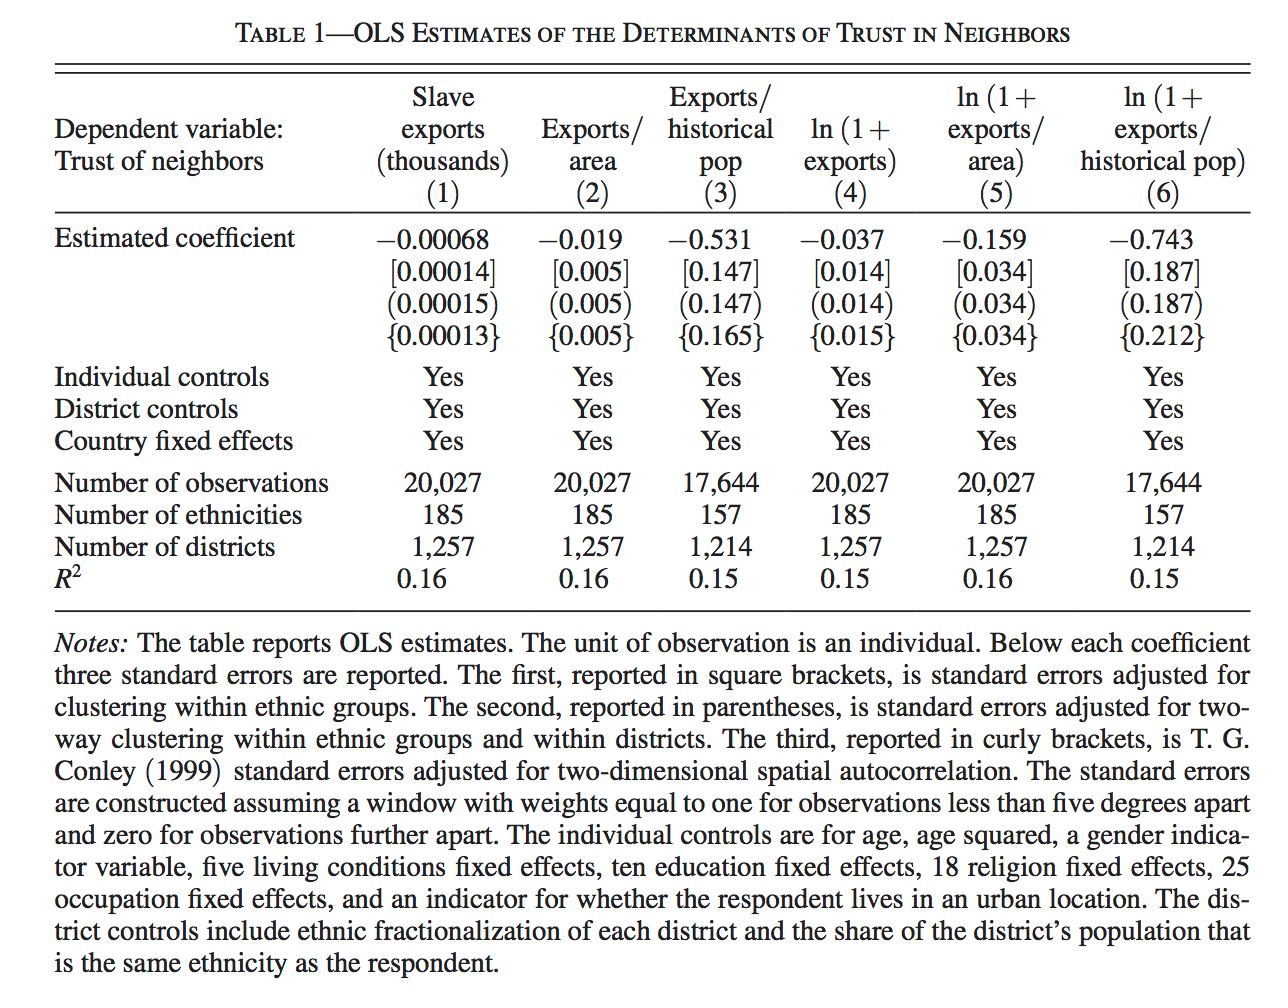
\includegraphics{images/nunn_wantchekon_table1.png}

A very crude way to describe regression is through linear combinations. The simplest linear combination is a one-to-one transformation.

Take the first number in Table 1, which is -0.00068. Now, multiply this by \texttt{exports}

\begin{Shaded}
\begin{Highlighting}[]
\FloatTok{-0.00068} \OperatorTok{*}\StringTok{ }\NormalTok{X[, }\StringTok{"exports"}\NormalTok{]}
\end{Highlighting}
\end{Shaded}

\begin{verbatim}
##  [1] -0.0002640778 -0.0004291640 -0.0006760487 -0.1241606061  0.0000000000
##  [6]  0.0000000000 -0.4528563428 -0.0002363964 -0.0002957912  0.0000000000
\end{verbatim}

Now, just one more step. Make a new matrix with just exports and the value 1

\begin{Shaded}
\begin{Highlighting}[]
\NormalTok{X2 <-}\StringTok{ }\KeywordTok{cbind}\NormalTok{(}\DecValTok{1}\NormalTok{, X[, }\StringTok{"exports"}\NormalTok{])}
\end{Highlighting}
\end{Shaded}

name this new column ``intercept''

\begin{Shaded}
\begin{Highlighting}[]
\KeywordTok{colnames}\NormalTok{(X2)}
\end{Highlighting}
\end{Shaded}

\begin{verbatim}
## NULL
\end{verbatim}

\begin{Shaded}
\begin{Highlighting}[]
\KeywordTok{colnames}\NormalTok{(X2) <-}\StringTok{ }\KeywordTok{c}\NormalTok{(}\StringTok{"intercept"}\NormalTok{, }\StringTok{"exports"}\NormalTok{)}
\end{Highlighting}
\end{Shaded}

What are the dimensions of the matrix \texttt{X2}?

\begin{Shaded}
\begin{Highlighting}[]
\KeywordTok{dim}\NormalTok{(X2)}
\end{Highlighting}
\end{Shaded}

\begin{verbatim}
## [1] 10  2
\end{verbatim}

Now consider a new matrix, called \texttt{B}.

\begin{Shaded}
\begin{Highlighting}[]
\NormalTok{B <-}\StringTok{ }\KeywordTok{matrix}\NormalTok{(}\KeywordTok{c}\NormalTok{(}\FloatTok{1.62}\NormalTok{, }\FloatTok{-0.00068}\NormalTok{))}
\end{Highlighting}
\end{Shaded}

What are the dimensions of \texttt{B}?

\begin{Shaded}
\begin{Highlighting}[]
\KeywordTok{dim}\NormalTok{(B)}
\end{Highlighting}
\end{Shaded}

\begin{verbatim}
## [1] 2 1
\end{verbatim}

What is the product of \texttt{X2} and \texttt{B}? From the dimensions, can you tell if it will be conformable?

\begin{Shaded}
\begin{Highlighting}[]
\NormalTok{X2 }\OperatorTok\StringTok{ }\NormalTok{B}
\end{Highlighting}
\end{Shaded}

\begin{verbatim}
##           [,1]
##  [1,] 1.619736
##  [2,] 1.619571
##  [3,] 1.619324
##  [4,] 1.495839
##  [5,] 1.620000
##  [6,] 1.620000
##  [7,] 1.167144
##  [8,] 1.619764
##  [9,] 1.619704
## [10,] 1.620000
\end{verbatim}

What is this multiplication doing in terms of equations?

\hypertarget{exercises-1}{%
\section*{Exercises}\label{exercises-1}}
\addcontentsline{toc}{section}{Exercises}

\hypertarget{section-9}{%
\subsection*{1}\label{section-9}}
\addcontentsline{toc}{subsection}{1}

Let
\[\mathbf{A} = \left[\begin{array}
{rrr}
0.6 & 0.2\\
0.4 & 0.8\\
\end{array}\right]
\]

Use R to write code that will create the matrix \(A\), and then consecutively multiply \(A\) to itself 4 times. What is the value of \(A^{4}\)?

\begin{Shaded}
\begin{Highlighting}[]
\CommentTok{## Enter yourself}
\end{Highlighting}
\end{Shaded}

Note that R notation of matrices is different from the math notation. Simply trying \texttt{X\^{}n} where \texttt{X} is a matrix will only take the power of each element to \texttt{n}. Instead, this problem asks you to perform matrix multiplication.

\hypertarget{section-10}{%
\subsection*{2}\label{section-10}}
\addcontentsline{toc}{subsection}{2}

Let's apply what we learned about subsetting or filtering/selecting. Use the \texttt{nunn\_full} dataset you have already loaded

\begin{enumerate}
\def\labelenumi{\alph{enumi})}
\tightlist
\item
  First, show all observations (rows) that have a \texttt{"male"} variable higher than 0.5
\end{enumerate}

\begin{Shaded}
\begin{Highlighting}[]
\CommentTok{## Enter yourself}
\end{Highlighting}
\end{Shaded}

\begin{enumerate}
\def\labelenumi{\alph{enumi})}
\setcounter{enumi}{1}
\tightlist
\item
  Next, create a matrix / dataframe with only two columns: \texttt{"trust\_neighbors"} and \texttt{"age"}
\end{enumerate}

\begin{Shaded}
\begin{Highlighting}[]
\CommentTok{## Enter yourself}
\end{Highlighting}
\end{Shaded}

\begin{enumerate}
\def\labelenumi{\alph{enumi})}
\setcounter{enumi}{2}
\tightlist
\item
  Lastly, show all values of \texttt{"trust\_neighbors"} and \texttt{"age"} for observations (rows) that have the ``male'' variable value that is higher than 0.5
\end{enumerate}

\begin{Shaded}
\begin{Highlighting}[]
\CommentTok{## Enter yourself}
\end{Highlighting}
\end{Shaded}

\hypertarget{section-11}{%
\subsection*{3}\label{section-11}}
\addcontentsline{toc}{subsection}{3}

Find a way to generate a vector of ``column averages'' of the matrix \texttt{X} from the Nunn and Wantchekon data in one line of code. Each entry in the vector should contain the sample average of the values in the column. So a 100 by 4 matrix should generate a length-4 matrix.

\hypertarget{section-12}{%
\subsection*{4}\label{section-12}}
\addcontentsline{toc}{subsection}{4}

Similarly, generate a vector of ``column medians''.

\hypertarget{section-13}{%
\subsection*{5}\label{section-13}}
\addcontentsline{toc}{subsection}{5}

Consider the regression that was run to generate Table 1:

\begin{Shaded}
\begin{Highlighting}[]
\NormalTok{form <-}\StringTok{ "trust_neighbors ~ exports + age + age2 +  male + urban_dum + factor(education) + factor(occupation) + factor(religion) + factor(living_conditions) + district_ethnic_frac + frac_ethnicity_in_district + isocode"}
\NormalTok{lm_}\DecValTok{1}\NormalTok{_}\DecValTok{1}\NormalTok{ <-}\StringTok{ }\KeywordTok{lm}\NormalTok{(}\KeywordTok{as.formula}\NormalTok{(form), nunn_full)}

\CommentTok{# The below coef function returns a vector of OLS coefficiants}
\KeywordTok{coef}\NormalTok{(lm_}\DecValTok{1}\NormalTok{_}\DecValTok{1}\NormalTok{)}
\end{Highlighting}
\end{Shaded}

\begin{verbatim}
##                (Intercept)                    exports 
##               1.619913e+00              -6.791360e-04 
##                        age                       age2 
##               8.395936e-03              -5.473436e-05 
##                       male                  urban_dum 
##               4.550246e-02              -1.404551e-01 
##         factor(education)1         factor(education)2 
##               1.709816e-02              -5.224591e-02 
##         factor(education)3         factor(education)4 
##              -1.373770e-01              -1.889619e-01 
##         factor(education)5         factor(education)6 
##              -1.893494e-01              -2.400767e-01 
##         factor(education)7         factor(education)8 
##              -2.850748e-01              -1.232085e-01 
##         factor(education)9        factor(occupation)1 
##              -2.406437e-01               6.185655e-02 
##        factor(occupation)2        factor(occupation)3 
##               7.392168e-02               3.356158e-02 
##        factor(occupation)4        factor(occupation)5 
##               7.942048e-03               6.661126e-02 
##        factor(occupation)6        factor(occupation)7 
##              -7.563297e-02               1.699699e-02 
##        factor(occupation)8        factor(occupation)9 
##              -9.428177e-02              -9.981440e-02 
##       factor(occupation)10       factor(occupation)11 
##              -3.307068e-02              -2.300045e-02 
##       factor(occupation)12       factor(occupation)13 
##              -1.564540e-01              -1.441370e-02 
##       factor(occupation)14       factor(occupation)15 
##              -5.566414e-02              -2.343762e-01 
##       factor(occupation)16       factor(occupation)18 
##              -1.306947e-02              -1.729589e-01 
##       factor(occupation)19       factor(occupation)20 
##              -1.770261e-01              -2.457800e-02 
##       factor(occupation)21       factor(occupation)22 
##              -4.936813e-02              -1.068511e-01 
##       factor(occupation)23       factor(occupation)24 
##              -9.712205e-02               1.292371e-02 
##       factor(occupation)25      factor(occupation)995 
##               2.623186e-02              -1.195063e-03 
##          factor(religion)2          factor(religion)3 
##               5.395953e-02               7.887878e-02 
##          factor(religion)4          factor(religion)5 
##               4.749150e-02               4.318455e-02 
##          factor(religion)6          factor(religion)7 
##              -1.787694e-02              -3.616542e-02 
##         factor(religion)10         factor(religion)11 
##               6.015041e-02               2.237845e-01 
##         factor(religion)12         factor(religion)13 
##               2.627086e-01              -6.812813e-02 
##         factor(religion)14         factor(religion)15 
##               4.673681e-02               3.844555e-01 
##        factor(religion)360        factor(religion)361 
##               3.656843e-01               3.416413e-01 
##        factor(religion)362        factor(religion)363 
##               8.230393e-01               3.856565e-01 
##        factor(religion)995 factor(living_conditions)2 
##               4.161301e-02               4.395862e-02 
## factor(living_conditions)3 factor(living_conditions)4 
##               8.627372e-02               1.197428e-01 
## factor(living_conditions)5       district_ethnic_frac 
##               1.203606e-01              -1.553648e-02 
## frac_ethnicity_in_district                 isocodeBWA 
##               1.011222e-01              -4.258953e-01 
##                 isocodeGHA                 isocodeKEN 
##               1.135307e-02              -1.819556e-01 
##                 isocodeLSO                 isocodeMDG 
##              -5.511200e-01              -3.315727e-01 
##                 isocodeMLI                 isocodeMOZ 
##               7.528101e-02               8.223730e-02 
##                 isocodeMWI                 isocodeNAM 
##               3.062497e-01              -1.397541e-01 
##                 isocodeNGA                 isocodeSEN 
##              -2.381525e-01               3.867371e-01 
##                 isocodeTZA                 isocodeUGA 
##               2.079366e-01              -6.443732e-02 
##                 isocodeZAF                 isocodeZMB 
##              -2.179153e-01              -2.172868e-01
\end{verbatim}

First, get a small subset of the nunn\_full dataset. This time, sample 20 rows and select for variables \texttt{exports}, \texttt{age}, \texttt{age2}, \texttt{male}, and \texttt{urban\_dum}. To this small subset, add (\texttt{bind\_cols()} in tidyverse or \texttt{cbind()} in base R) a column of 1's; this represents the intercept. If you need some guidance, look at how we sampled 10 rows selected for a different set of variables above in the lecture portion.

\begin{Shaded}
\begin{Highlighting}[]
\CommentTok{# Enter here}
\end{Highlighting}
\end{Shaded}

Next let's try calculating predicted values of levels of trust in neighbors by multiplying coefficients for the intercept, \texttt{exports}, \texttt{age}, \texttt{age2}, \texttt{male}, and \texttt{urban\_dum} to the actual observed values for those variables in the small subset you've just created.

\begin{Shaded}
\begin{Highlighting}[]
\CommentTok{# Hint: You can get just selected elements from the vector returned by coef(lm_1_1)}

\CommentTok{# For example, the below code gives you the first 3 elements of the original vector}
\KeywordTok{coef}\NormalTok{(lm_}\DecValTok{1}\NormalTok{_}\DecValTok{1}\NormalTok{)[}\DecValTok{1}\OperatorTok{:}\DecValTok{3}\NormalTok{]}
\end{Highlighting}
\end{Shaded}

\begin{verbatim}
##  (Intercept)      exports          age 
##  1.619913146 -0.000679136  0.008395936
\end{verbatim}

\begin{Shaded}
\begin{Highlighting}[]
\CommentTok{# Also, the below code gives you the coefficient elements for intercept and male}
\KeywordTok{coef}\NormalTok{(lm_}\DecValTok{1}\NormalTok{_}\DecValTok{1}\NormalTok{)[}\KeywordTok{c}\NormalTok{(}\StringTok{"(Intercept)"}\NormalTok{, }\StringTok{"male"}\NormalTok{)]}
\end{Highlighting}
\end{Shaded}

\begin{verbatim}
## (Intercept)        male 
##  1.61991315  0.04550246
\end{verbatim}

\hypertarget{dataviz}{%
\chapter[Visualization]{\texorpdfstring{Visualization\footnote{Module originally written by Shiro Kuriwaki}}{Visualization}}\label{dataviz}}

\hypertarget{where-are-we-where-are-we-headed-2}{%
\subsection*{Where are we? Where are we headed?}\label{where-are-we-where-are-we-headed-2}}
\addcontentsline{toc}{subsection}{Where are we? Where are we headed?}

Up till now, you should have covered:

\begin{itemize}
\tightlist
\item
  The R Visualization and Programming primers at \url{https://rstudio.cloud/primers/}
\item
  Reading and handling data
\item
  Matrices and Vectors

  \begin{itemize}
  \tightlist
  \item
    What does \texttt{:} mean in R? What about \texttt{==}? \texttt{,}?, \texttt{!=} , \texttt{\&}, \texttt{\textbar{}}, \texttt{\%in\%}
  \item
    What does \texttt{\%\textgreater{}\%} do?
  \end{itemize}
\end{itemize}

Today we'll cover:

\begin{itemize}
\tightlist
\item
  Visualization
\item
  A bit of data wrangling
\end{itemize}

\hypertarget{check-your-understanding-1}{%
\subsection*{Check your understanding}\label{check-your-understanding-1}}
\addcontentsline{toc}{subsection}{Check your understanding}

\begin{itemize}
\tightlist
\item
  How do you make a barplot, in base-R and in ggplot?
\item
  How do you add layers to a ggplot?
\item
  How do you change the axes of a ggplot?
\item
  How do you make a histogram?
\item
  How do you make a graph that looks like this?
\end{itemize}

\begin{figure}
\centering
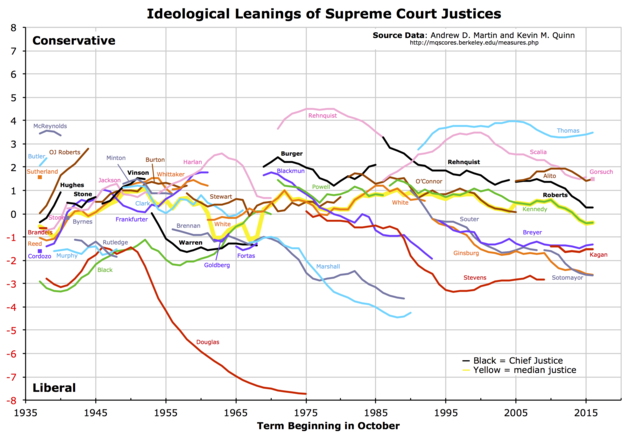
\includegraphics{images/Martin-Quinn_Wikipedia.png}
\caption{By Randy Schutt - Own work, CC BY-SA 3.0, \href{https://commons.wikimedia.org/w/index.php?curid=29585342}{Wikimedia.}}
\end{figure}

Other review

\hypertarget{motivation-the-law-of-the-census}{%
\section{Motivation: The Law of the Census}\label{motivation-the-law-of-the-census}}

In this module, let's visualize some cross-sectional stats with an actual Census. Then, we'll do an example on time trends with Supreme Court ideal points.

Why care about the Census? The Census is one of the fundamental acts of a government. See the Law Review article by \href{http://cardozolawreview.com/Joomla1.5/content/32-3/Persily.32-3.pdf}{Persily (2011)}, ``The Law of the Census.''\footnote{\href{http://cardozolawreview.com/Joomla1.5/content/32-3/Persily.32-3.pdf}{Persily, Nathaniel. 2011. ``The Law of the Census: How to Count, What to Count, Whom to Count, and Where to Count Them.''}. \emph{Cardozo Law Review} 32(3): 755--91.} The Census is government's primary tool for apportionment (allocating seats to districts), appropriations (allocating federal funding), and tracking demographic change. See\footnote{\href{https://dash.harvard.edu/bitstream/handle/1/3153295/hoschschild_racialreorganization.pdf?sequence=2}{Hochschild, Jennifer L., and Brenna Marea Powell. 2008. ``Racial Reorganization and the United States Census 1850--1930: Mulattoes, Half-Breeds, Mixed Parentage, Hindoos, and the Mexican Race.''}. \emph{Studies in American Political Development} 22(1): 59--96.} for example \href{https://dash.harvard.edu/bitstream/handle/1/3153295/hoschschild_racialreorganization.pdf?sequence=2}{Hochschild and Powell (2008)} on how the categorizations of race in the Census during 1850-1930. Notice also that both of these pieces are not inherently ``quantitative'' --- the Persily article is a Law Review and the Hochschild and Powell article is on American Historical Development --- but data analysis would be certainly relevant.

Time series data is a common form of data in social science data, and there is growing methodological work on making causal inferences with time series.\footnote{\href{https://doi.org/10.1017/S0003055418000357}{Blackwell, Matthew, and Adam Glynn. 2018. ``How to Make Causal Inferences with Time-Series Cross-Sectional Data under Selection on Observables.''} \emph{American Political Science Review}} We will use the the ideological estimates of the Supreme court, which has been in the news with Brett Kavanaugh's nomination.

\hypertarget{read-data-2}{%
\section{Read data}\label{read-data-2}}

First, the census. Read in a subset of the 2010 Census. This is a 1 percent sample of the entire U.S. Census (100 times larger than the previous version).

\begin{Shaded}
\begin{Highlighting}[]
\NormalTok{cen10 <-}\StringTok{ }\KeywordTok{readRDS}\NormalTok{(}\StringTok{"input/usc2010_1percent.Rds"}\NormalTok{)}
\end{Highlighting}
\end{Shaded}

The data comes from IPUMS\footnote{\href{http://doi.org/10.18128/D010.V6.0}{Ruggles, Steven, Katie Genadek, Ronald Goeken, Josiah Grover, and Matthew Sobek. 2015. Integrated Public Use Microdata Series: Version 6.0 dataset}}, a great source to extract and analyze Census and Census-conducted survey (ACS, CPS) data.

\hypertarget{counting}{%
\section{Counting}\label{counting}}

How many people are in your sample?

\begin{Shaded}
\begin{Highlighting}[]
\KeywordTok{nrow}\NormalTok{(cen10)}
\end{Highlighting}
\end{Shaded}

\begin{verbatim}
## [1] 3087108
\end{verbatim}

This and all subsequent tasks involve manipulating and summarizing data, sometimes called ``wrangling''. As per last time, there are both ``base-R'' and ``tidyverse'' approaches.

Yesterday we saw several functions from the tidyverse:

\begin{itemize}
\tightlist
\item
  \texttt{select} selects columns
\item
  \texttt{filter} selects rows based on a logical (boolean) statement
\item
  \texttt{slice} selects rows based on the row number
\item
  \texttt{arrange} reordered the rows in descending order.
\end{itemize}

In this visualization section, we'll make use of the pair of functions \texttt{group\_by()} and \texttt{summarize()}.

\hypertarget{tabulating}{%
\section{Tabulating}\label{tabulating}}

Summarizing data is the key part of communication; good data viz gets the point across.\footnote{\href{http://www.princeton.edu/~jkastell/Tables2Graphs/graphs.pdf}{Kastellec, Jonathan P., and Eduardo L. Leoni. 2007. ``Using Graphs Instead of Tables in Political Science.''}. \emph{Perspectives on Politics} 5 (4): 755--71.} Summaries of data come in two forms: tables and figures.

Here are two ways to count by group, or to tabulate.

In base-R Use the \texttt{table} function, that provides how many rows exist for an unique value of the vector (remember \texttt{unique} from yesterday?)

\begin{Shaded}
\begin{Highlighting}[]
\KeywordTok{table}\NormalTok{(cen10}\OperatorTok{$}\NormalTok{race)}
\end{Highlighting}
\end{Shaded}

\begin{verbatim}
## 
## American Indian or Alaska Native     Black/African American/Negro 
##                            29584                           390640 
##                          Chinese                         Japanese 
##                            33537                             7629 
##  Other Asian or Pacific Islander                  Other race, nec 
##                           110325                           190319 
##        Three or more major races                  Two major races 
##                             8421                            82724 
##                            White 
##                          2233929
\end{verbatim}

With tidyverse, a quick convenience function is \texttt{count}, with the variable to count on included.

\begin{Shaded}
\begin{Highlighting}[]
\KeywordTok{count}\NormalTok{(cen10, race)}
\end{Highlighting}
\end{Shaded}

\begin{verbatim}
## # A tibble: 9 x 2
##   race                                   n
##   <chr>                              <int>
## 1 American Indian or Alaska Native   29584
## 2 Black/African American/Negro      390640
## 3 Chinese                            33537
## 4 Japanese                            7629
## 5 Other Asian or Pacific Islander   110325
## 6 Other race, nec                   190319
## 7 Three or more major races           8421
## 8 Two major races                    82724
## 9 White                            2233929
\end{verbatim}

We can check out the arguments of \texttt{count} and see that there is a \texttt{sort} option. What does this do?

\begin{Shaded}
\begin{Highlighting}[]
\KeywordTok{count}\NormalTok{(cen10, race, }\DataTypeTok{sort =} \OtherTok{TRUE}\NormalTok{)}
\end{Highlighting}
\end{Shaded}

\begin{verbatim}
## # A tibble: 9 x 2
##   race                                   n
##   <chr>                              <int>
## 1 White                            2233929
## 2 Black/African American/Negro      390640
## 3 Other race, nec                   190319
## 4 Other Asian or Pacific Islander   110325
## 5 Two major races                    82724
## 6 Chinese                            33537
## 7 American Indian or Alaska Native   29584
## 8 Three or more major races           8421
## 9 Japanese                            7629
\end{verbatim}

\texttt{count} is a kind of shorthand for \texttt{group\_by()} and \texttt{summarize}. This code would have done the same.

\begin{Shaded}
\begin{Highlighting}[]
\NormalTok{cen10 }\OperatorTok\StringTok{ }
\StringTok{  }\KeywordTok{group_by}\NormalTok{(race) }\OperatorTok\StringTok{ }
\StringTok{  }\KeywordTok{summarize}\NormalTok{(}\DataTypeTok{n =} \KeywordTok{n}\NormalTok{())}
\end{Highlighting}
\end{Shaded}

\begin{verbatim}
## # A tibble: 9 x 2
##   race                                   n
##   <chr>                              <int>
## 1 American Indian or Alaska Native   29584
## 2 Black/African American/Negro      390640
## 3 Chinese                            33537
## 4 Japanese                            7629
## 5 Other Asian or Pacific Islander   110325
## 6 Other race, nec                   190319
## 7 Three or more major races           8421
## 8 Two major races                    82724
## 9 White                            2233929
\end{verbatim}

If you are new to tidyverse, what would you \emph{think} each row did? Reading the function help page, verify if your intuition was correct.

where \texttt{n()} is a function that counts rows.

\hypertarget{base-r-graphics-and-ggplot}{%
\section{base R graphics and ggplot}\label{base-r-graphics-and-ggplot}}

Two prevalent ways of making graphing are referred to as ``base-R'' and ``ggplot''.

\hypertarget{base-r}{%
\subsection{base R}\label{base-r}}

``Base-R'' graphics are graphics that are made with R's default graphics commands. First, let's assign our tabulation to an object,
then put it in the \texttt{barplot()} function.

\begin{Shaded}
\begin{Highlighting}[]
\KeywordTok{barplot}\NormalTok{(}\KeywordTok{table}\NormalTok{(cen10}\OperatorTok{$}\NormalTok{race))}
\end{Highlighting}
\end{Shaded}

\includegraphics{prefresher_files/figure-latex/unnamed-chunk-178-1.pdf}

\hypertarget{ggplot}{%
\subsection{ggplot}\label{ggplot}}

A popular alternative a \texttt{ggplot} graphics, that you were introduced to in the tutorial. \texttt{gg} stands for grammar of graphics by Hadley Wickham, and it has a new semantics of explaining graphics in R. Again, first let's set up the data.

Although the tutorial covered making scatter plots as the first cut, often data requires summaries before they made into graphs.

For this example, let's group and count first like we just did. But assign it to a new object.

\begin{Shaded}
\begin{Highlighting}[]
\NormalTok{grp_race <-}\StringTok{ }\KeywordTok{count}\NormalTok{(cen10, race)}
\end{Highlighting}
\end{Shaded}

We will now plot this grouped set of numbers. Recall that the \texttt{ggplot()} function takes two main arguments, \texttt{data} and \texttt{aes}.

\begin{enumerate}
\def\labelenumi{\arabic{enumi}.}
\tightlist
\item
  First enter a single dataframe from which you will draw a plot.
\item
  Then enter the \texttt{aes}, or aesthetics. This defines which variable in the data the plotting functions should take for pre-set dimensions in graphics. The dimensions \texttt{x} and \texttt{y} are the most important. We will assign \texttt{race} and \texttt{count} to them, respectively,
\item
  After you close \texttt{ggplot()} .. add \textbf{layers} by the plus sign. A \texttt{geom} is a layer of graphical representation, for example \texttt{geom\_histogram} renders a histogram, \texttt{geom\_point} renders a scatter plot. For a barplot, we can use \texttt{geom\_col()}
\end{enumerate}

What is the right geometry layer to make a barplot? Turns out:

\begin{Shaded}
\begin{Highlighting}[]
\KeywordTok{ggplot}\NormalTok{(}\DataTypeTok{data =}\NormalTok{ grp_race, }\KeywordTok{aes}\NormalTok{(}\DataTypeTok{x =}\NormalTok{ race, }\DataTypeTok{y =}\NormalTok{ n)) }\OperatorTok{+}\StringTok{ }\KeywordTok{geom_col}\NormalTok{()}
\end{Highlighting}
\end{Shaded}

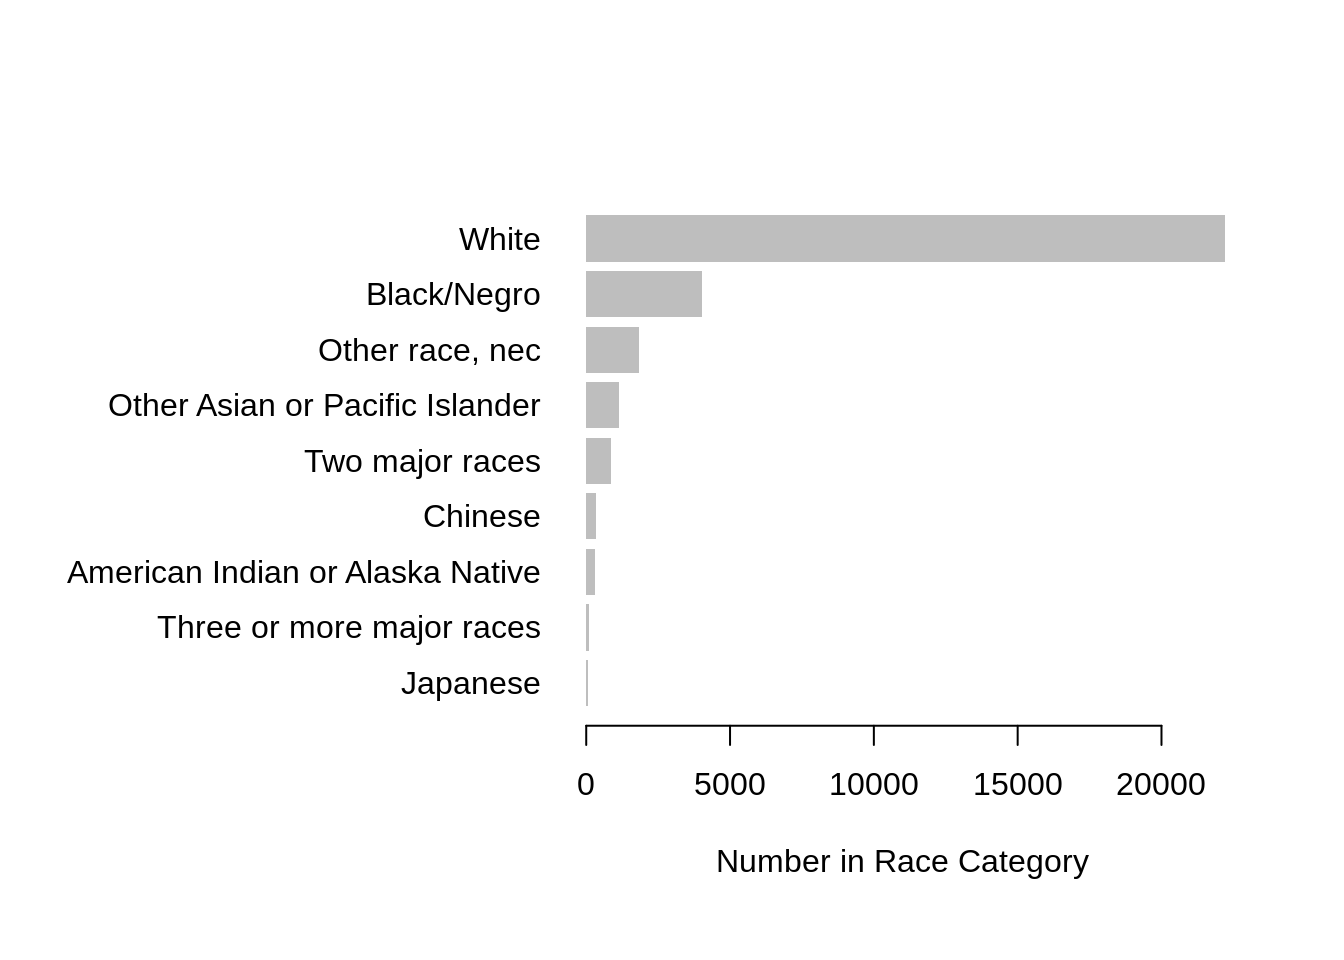
\includegraphics{prefresher_files/figure-latex/unnamed-chunk-180-1.pdf}

\hypertarget{improving-your-graphics}{%
\section{Improving your graphics}\label{improving-your-graphics}}

Adjusting your graphics to make the point clear is an important skill. Here is a base-R example of showing the same numbers but with a different design, in a way that aims to maximize the ``data-to-ink ratio''.

\begin{Shaded}
\begin{Highlighting}[]
\KeywordTok{par}\NormalTok{(}\DataTypeTok{oma =} \KeywordTok{c}\NormalTok{(}\DecValTok{1}\NormalTok{, }\DecValTok{11}\NormalTok{, }\DecValTok{1}\NormalTok{, }\DecValTok{1}\NormalTok{))}
\KeywordTok{barplot}\NormalTok{(}\KeywordTok{sort}\NormalTok{(}\KeywordTok{table}\NormalTok{(cen10}\OperatorTok{$}\NormalTok{race)), }\CommentTok{# sort numbers}
        \DataTypeTok{horiz =} \OtherTok{TRUE}\NormalTok{, }\CommentTok{# flip}
        \DataTypeTok{border =} \OtherTok{NA}\NormalTok{, }\CommentTok{# border is extraneous}
        \DataTypeTok{xlab =} \StringTok{"Number in Race Category"}\NormalTok{, }
        \DataTypeTok{bty =} \StringTok{"n"}\NormalTok{, }\CommentTok{# no box}
        \DataTypeTok{las =} \DecValTok{1}\NormalTok{) }\CommentTok{# alignment of axis labels is horizontal}
\end{Highlighting}
\end{Shaded}

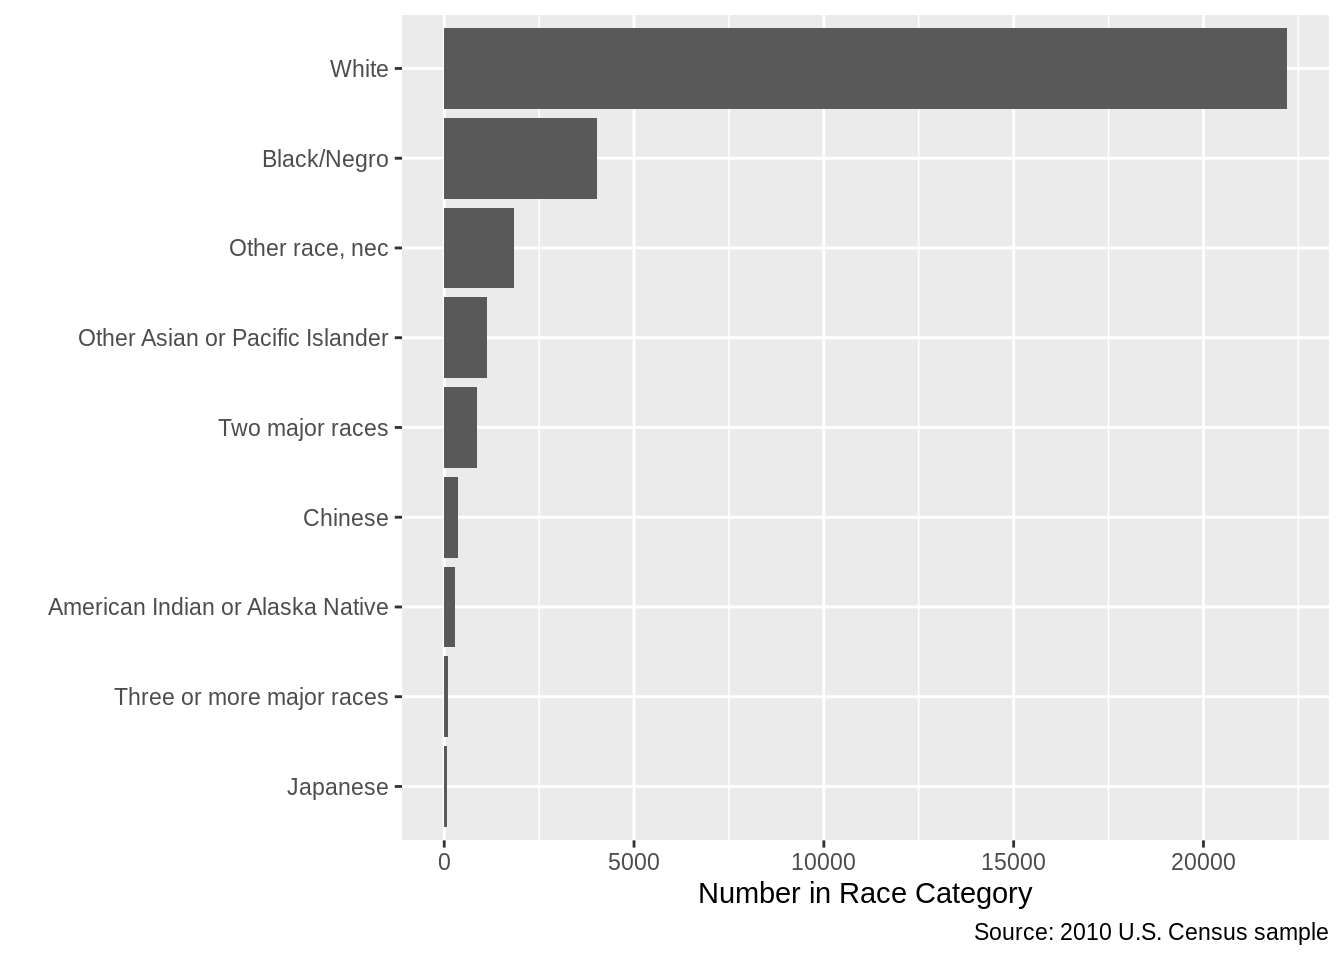
\includegraphics{prefresher_files/figure-latex/unnamed-chunk-181-1.pdf}

Notice that we applied the \texttt{sort()} function to order the bars in terms of their counts. The default ordering of a categorical variable / factor is alphabetical. Alphabetical ordering is uninformative and almost never the way you should order variables.

In ggplot you might do this by:

\begin{Shaded}
\begin{Highlighting}[]
\KeywordTok{library}\NormalTok{(forcats)}

\NormalTok{grp_race_ordered <-}\StringTok{ }\KeywordTok{arrange}\NormalTok{(grp_race, n) }\OperatorTok\StringTok{ }
\StringTok{  }\KeywordTok{mutate}\NormalTok{(}\DataTypeTok{race =} \KeywordTok{as_factor}\NormalTok{(race))}

\KeywordTok{ggplot}\NormalTok{(}\DataTypeTok{data =}\NormalTok{ grp_race_ordered, }\KeywordTok{aes}\NormalTok{(}\DataTypeTok{x =}\NormalTok{ race, }\DataTypeTok{y =}\NormalTok{ n)) }\OperatorTok{+}
\StringTok{  }\KeywordTok{geom_col}\NormalTok{() }\OperatorTok{+}
\StringTok{  }\KeywordTok{coord_flip}\NormalTok{() }\OperatorTok{+}
\StringTok{  }\KeywordTok{labs}\NormalTok{(}\DataTypeTok{y =} \StringTok{"Number in Race Category"}\NormalTok{,}
       \DataTypeTok{x =} \StringTok{""}\NormalTok{,}
       \DataTypeTok{caption =} \StringTok{"Source: 2010 U.S. Census sample"}\NormalTok{)}
\end{Highlighting}
\end{Shaded}

\includegraphics{prefresher_files/figure-latex/unnamed-chunk-182-1.pdf}

The data ink ratio was popularized by Ed Tufte (originally a political economy scholar who has recently become well known for his data visualization work). See Tufte (2001), \emph{The Visual Display of Quantitative Information} and his website \url{https://www.edwardtufte.com/tufte/}. For a R and ggplot focused example using social science examples, check out Healy (2018), \emph{Data Visualization: A Practical Introduction} with a draft at \url{https://socviz.co/}\footnote{Healy, Kieran. forthcoming. \emph{Data Visualization: A Practical Introduction}. Princeton University Press}. There are a growing number of excellent books on data visualization.

\hypertarget{cross-tabs}{%
\section{Cross-tabs}\label{cross-tabs}}

Visualizations and Tables each have their strengths. A rule of thumb is that more than a dozen numbers on a table is too much to digest, but less than a dozen is too few for a figure to be worth it. Let's look at a table first.

A cross-tab is counting with two types of variables, and is a simple and powerful tool to show the relationship between multiple variables.

\begin{Shaded}
\begin{Highlighting}[]
\NormalTok{xtab_race_state <-}\StringTok{ }\KeywordTok{table}\NormalTok{(cen10}\OperatorTok{$}\NormalTok{state, cen10}\OperatorTok{$}\NormalTok{race)}
\end{Highlighting}
\end{Shaded}

What would the dimensions of this table be?

What if we care about proportions within states, rather than counts. We want to compare the racial composition of a small state (like Delaware) and a large state (like California).

One way to transform a table of counts to a table of proportions is the function \texttt{prop.table}. Be careful what you want to take proportions of -- this is set by the \texttt{margin} argument. In R, the first margin (\texttt{margin\ =\ 1}) is \emph{rows} and the second (\texttt{margin\ =\ 2}) is \emph{columns}.

\begin{Shaded}
\begin{Highlighting}[]
\NormalTok{ptab_race_state <-}\StringTok{ }\KeywordTok{prop.table}\NormalTok{(xtab_race_state, }\DataTypeTok{margin =} \DecValTok{2}\NormalTok{)}
\end{Highlighting}
\end{Shaded}

\hypertarget{composition-plots}{%
\section{Composition Plots}\label{composition-plots}}

How would you make the same figure with \texttt{ggplot()}? First, we want a count for each state \(\times\) race combination. So group by those two factors and count how many observations are in each two-way categorization. \texttt{group\_by()} can take any number of variables, separated by commas.

\begin{Shaded}
\begin{Highlighting}[]
\NormalTok{grp_race_state <-}\StringTok{ }\NormalTok{cen10 }\OperatorTok\StringTok{ }
\StringTok{  }\KeywordTok{count}\NormalTok{(race, state)}
\end{Highlighting}
\end{Shaded}

Can you tell from the code what \texttt{grp\_race\_state} will look like?

\begin{Shaded}
\begin{Highlighting}[]
\CommentTok{# run on your own}
\NormalTok{grp_race_state}
\end{Highlighting}
\end{Shaded}

Now, we want to tell \texttt{ggplot2} something like the following: I want bars by state, where heights indicate racial groups. Each bar should be colored by the race. With some googling, you will get something like this:

\begin{Shaded}
\begin{Highlighting}[]
\KeywordTok{ggplot}\NormalTok{(}\DataTypeTok{data =}\NormalTok{ grp_race_state, }\KeywordTok{aes}\NormalTok{(}\DataTypeTok{x =}\NormalTok{  state, }\DataTypeTok{y =}\NormalTok{ n,  }\DataTypeTok{fill =}\NormalTok{ race)) }\OperatorTok{+}
\StringTok{  }\KeywordTok{geom_col}\NormalTok{(}\DataTypeTok{position =} \StringTok{"fill"}\NormalTok{) }\OperatorTok{+}\StringTok{ }\CommentTok{# the position is dertemined by the fill ae}
\StringTok{  }\KeywordTok{scale_fill_brewer}\NormalTok{(}\DataTypeTok{name =} \StringTok{"Census Race"}\NormalTok{, }\DataTypeTok{palette =} \StringTok{"OrRd"}\NormalTok{, }\DataTypeTok{direction =} \DecValTok{-1}\NormalTok{) }\OperatorTok{+}\StringTok{ }\CommentTok{# choose palette}
\StringTok{  }\KeywordTok{coord_flip}\NormalTok{() }\OperatorTok{+}\StringTok{ }\CommentTok{# flip axes}
\StringTok{  }\KeywordTok{scale_y_continuous}\NormalTok{(}\DataTypeTok{labels =}\NormalTok{ percent) }\OperatorTok{+}\StringTok{ }\CommentTok{# label numbers as percentage}
\StringTok{  }\KeywordTok{labs}\NormalTok{(}\DataTypeTok{y =} \StringTok{"Proportion of Racial Group within State"}\NormalTok{,}
       \DataTypeTok{x =} \StringTok{""}\NormalTok{,}
       \DataTypeTok{source =} \StringTok{"Source: 2010 Census  sample"}\NormalTok{) }\OperatorTok{+}
\StringTok{  }\KeywordTok{theme_minimal}\NormalTok{()}
\end{Highlighting}
\end{Shaded}

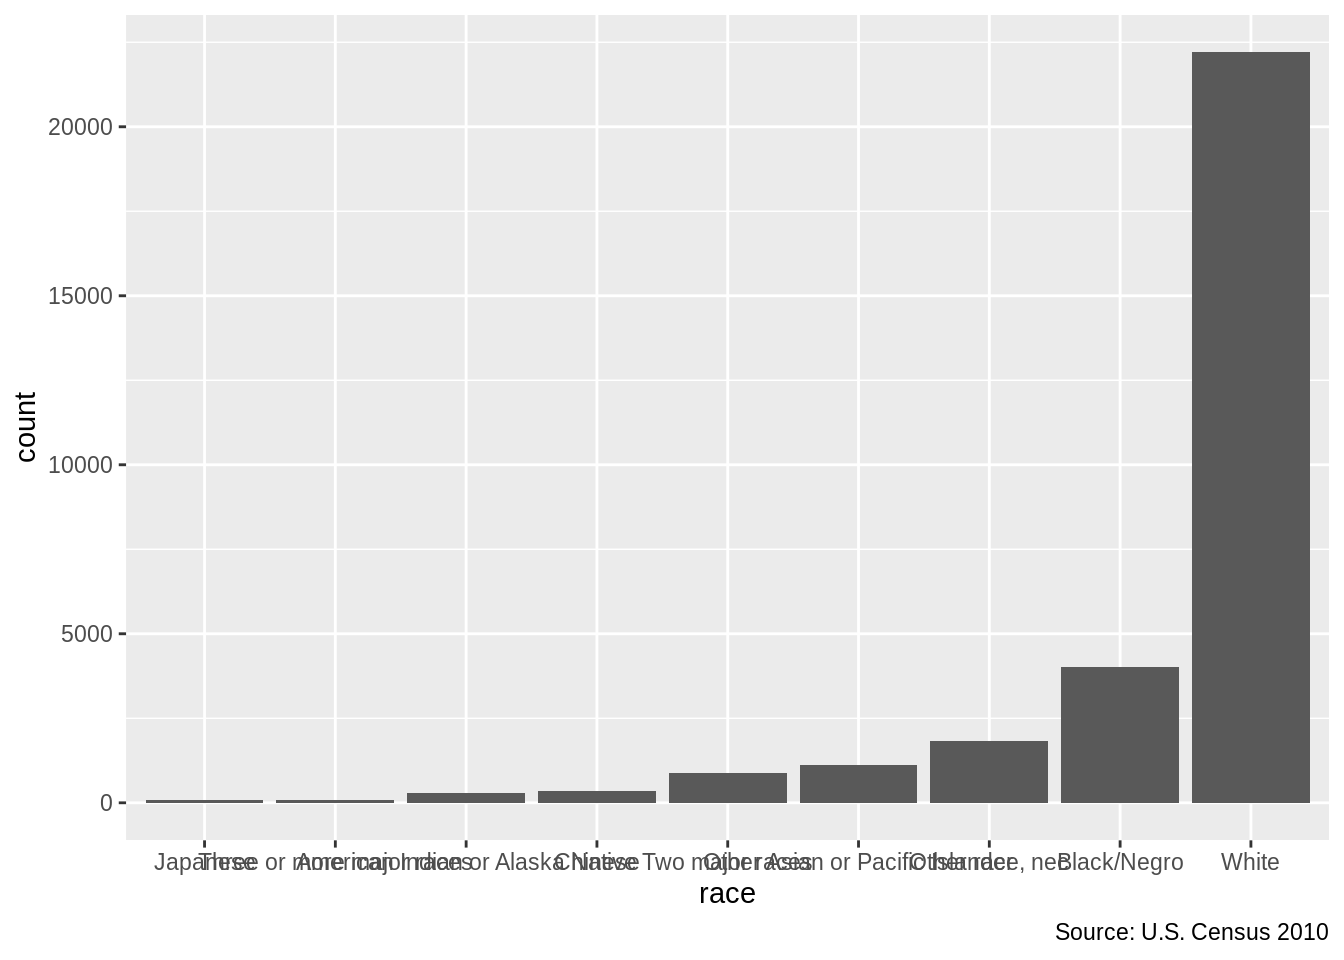
\includegraphics{prefresher_files/figure-latex/unnamed-chunk-187-1.pdf}

\hypertarget{line-graphs}{%
\section{Line graphs}\label{line-graphs}}

Line graphs are useful for plotting time trends.

The Census does not track individuals over time. So let's take up another example: The U.S. Supreme Court. Take the dataset \texttt{justices\_median.csv}.

This data is adapted from the estimates of Martin and Quinn on their website \url{http://mqscores.lsa.umich.edu/}.\footnote{This exercise inspired from Princeton's R Camp Assignment.}

\begin{Shaded}
\begin{Highlighting}[]
\NormalTok{justice <-}\StringTok{ }\KeywordTok{read_csv}\NormalTok{(}\StringTok{"input/justices_court-median.csv"}\NormalTok{)}
\end{Highlighting}
\end{Shaded}

What does the data look like? How do you think it is organized? What does each row represent?

\begin{Shaded}
\begin{Highlighting}[]
\NormalTok{justice}
\end{Highlighting}
\end{Shaded}

\begin{verbatim}
## # A tibble: 728 x 7
##     term justice_id justice idealpt idealpt_sd median_idealpt
##    <dbl>      <dbl> <chr>     <dbl>      <dbl>          <dbl>
##  1  1937         67 McReyn~   3.44       0.546         NA    
##  2  1938         67 McReyn~   3.57       0.561         NA    
##  3  1939         67 McReyn~   3.54       0.616         -1.07 
##  4  1940         67 McReyn~   3.36       0.714         -0.734
##  5  1937         68 Brande~  -0.611      0.273         NA    
##  6  1938         68 Brande~  -0.616      0.313         NA    
##  7  1937         71 Suther~   1.58       0.551         NA    
##  8  1937         72 Butler    2.07       0.425         NA    
##  9  1938         72 Butler    2.37       0.429         NA    
## 10  1937         74 Stone    -0.769      0.259         NA    
## # ... with 718 more rows, and 1 more variable: median_justice <chr>
\end{verbatim}

As you might have guessed, these data can be shown in a time trend from the range of the \texttt{term} variable. As there are only nine justices at any given time and justices have life tenure, there times on the court are staggered. With a common measure of ``preference'', we can plot time trends of these justices ideal points on the same y-axis scale.

\begin{Shaded}
\begin{Highlighting}[]
\KeywordTok{ggplot}\NormalTok{(justice, }\KeywordTok{aes}\NormalTok{(}\DataTypeTok{x =}\NormalTok{ term, }\DataTypeTok{y =}\NormalTok{ idealpt)) }\OperatorTok{+}
\StringTok{  }\KeywordTok{geom_line}\NormalTok{()}
\end{Highlighting}
\end{Shaded}

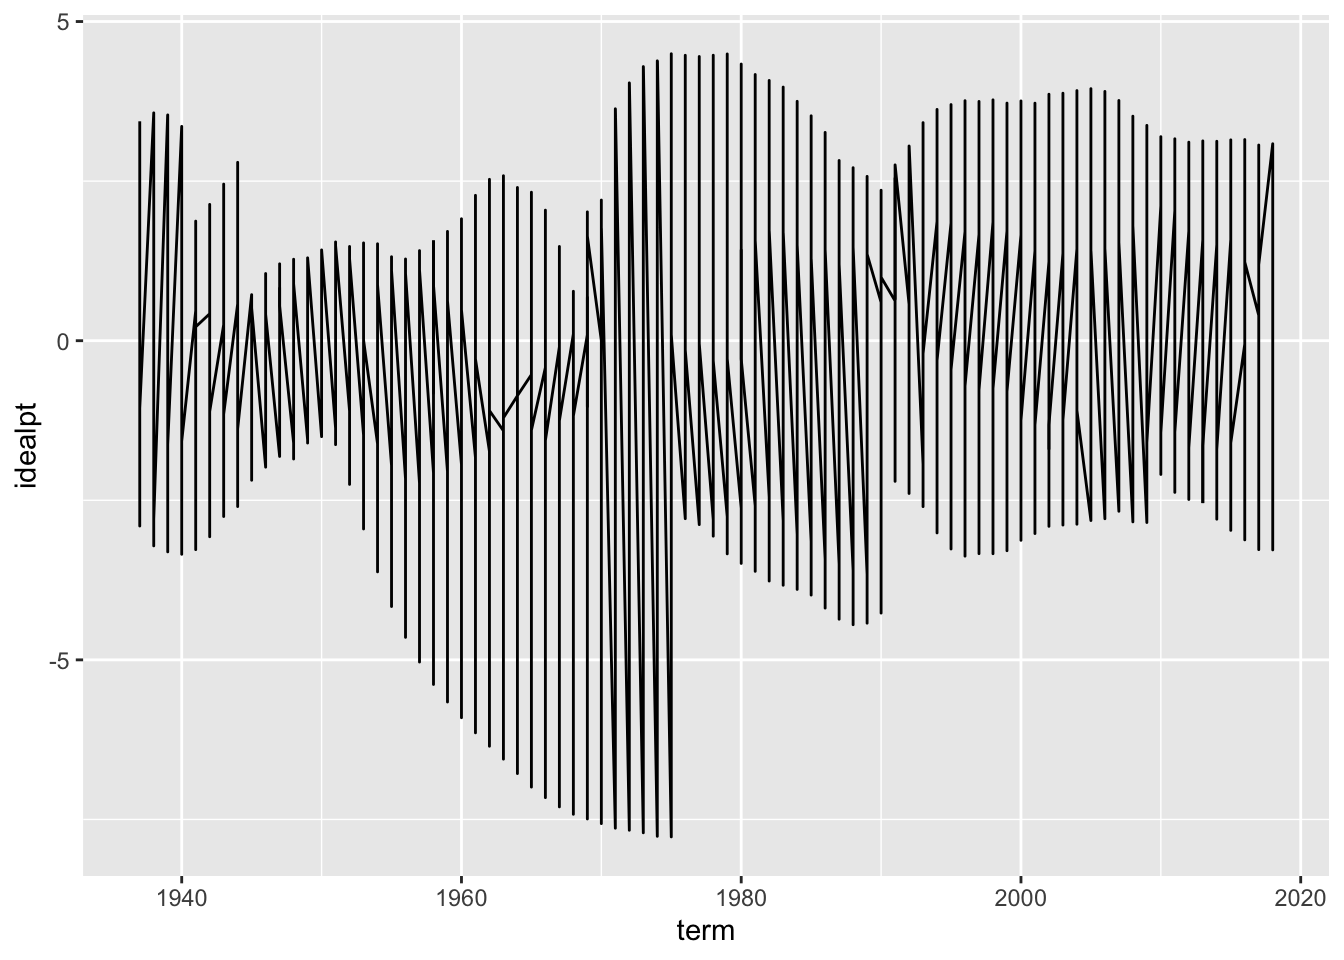
\includegraphics{prefresher_files/figure-latex/unnamed-chunk-190-1.pdf}
Why does the above graph not look like the the put in the beginning? Fix it by adding just one aesthetic to the graph.

\begin{Shaded}
\begin{Highlighting}[]
\CommentTok{# enter a correction that draws separate lines by group.}
\end{Highlighting}
\end{Shaded}

If you got the right aesthetic, this seems to ``work'' off the shelf. But take a moment to see why the code was written as it is and how that maps on to the graphics. What is the \texttt{group} aesthetic doing for you?

Now, this graphic already indicates a lot, but let's improve the graphics so people can actually read it. This is left for a Exercise.

As social scientists, we should also not forget to ask ourselves whether these numerical measures are fit for what we care about, or actually succeeds in measuring what we'd like to measure. The estimation of these ``ideal points'' is a subfield of political methodology beyond this prefresher. For more reading, skim through the original paper by Martin and Quinn (2002).\footnote{\href{http://mqscores.lsa.umich.edu/media/pa02.pdf}{Martin, Andrew D. and Kevin M. Quinn. 2002. ``Dynamic Ideal Point Estimation via Markov Chain Monte Carlo for the U.S. Supreme Court, 1953-1999''}. \emph{Political Analysis.} 10(2): 134-153.} Also for a methodological discussion on the difficulty of measuring time series of preferences, check out Bailey (2013).\footnote{\href{https://michaelbailey.georgetown.domains/wp-content/uploads/2018/05/JOP_proofs_June2013.pdf}{Bailey, Michael A. 2013. ``Is Today's Court the Most Conservative in Sixty Years? Challenges and Opportunities in Measuring Judicial Preferences.''}. \emph{Journal of Politics} 75(3): 821-834}

\hypertarget{exercises-2}{%
\section*{Exercises}\label{exercises-2}}
\addcontentsline{toc}{section}{Exercises}

In the time remaining, try the following exercises. Order doesn't matter.

\hypertarget{rural-states}{%
\subsection*{1: Rural states}\label{rural-states}}
\addcontentsline{toc}{subsection}{1: Rural states}

Make a well-labelled figure that plots the proportion of the state's population (as per the census) that reside in their file as a renter. Each state should be visualized as a point, rather than a bar, and there should be 51 points, ordered by their value. All labels should be readable.

\begin{Shaded}
\begin{Highlighting}[]
\CommentTok{# Enter yourself}
\end{Highlighting}
\end{Shaded}

\begin{itemize}
\tightlist
\item
  Alternatively, you can for instead plot the proportion of residents who do not reisde in a specified city.
\end{itemize}

\hypertarget{the-swing-justice}{%
\subsection*{2: The swing justice}\label{the-swing-justice}}
\addcontentsline{toc}{subsection}{2: The swing justice}

Using the \texttt{justice} dataset and building off of the plot that was given, make an improved plot by implementing as many of the following changes (which hopefully improves the graph):

\begin{itemize}
\tightlist
\item
  Label axes
\item
  Use a black-white background.
\item
  Change the breaks of the x-axis to print numbers for every decade, not just every two decades.
\item
  Plots each line in translucent gray, so the overlapping lines can be visualized clearly. (Hint: in ggplot the \texttt{alpha} argument controls the degree of transparency)
\item
  Limit the scale of the y-axis to {[}-5, 5{]} so that the outlier justice in the 60s is trimmed and the rest of the data can be seen more easily (also, who is that justice?)
\item
  Plot the ideal point of the justice who holds the ``median'' ideal point in a given term. To distinguish this with the others, plot this line separately in a very light red \emph{below} the individual justice's lines.
\item
  Highlight the trend-line of only the nine justices who are \emph{currently} sitting on SCOTUS. Make sure this is clearer than the other past justices.
\item
  Add the current nine justice's names to the right of the endpoint of the 2016 figure, alongside their ideal point.
\item
  Make sure the text labels do not overlap with each other for readability using the \texttt{ggrepel} package.
\item
  Extend the x-axis label to about 2020 so the text labels of justices are to the right of the trend-lines.
\item
  Add a caption to your text describing the data briefly, as well as any features relevant for the reader (such as the median line and the trimming of the y-axis)
\end{itemize}

\begin{Shaded}
\begin{Highlighting}[]
\CommentTok{# Enter yourself}
\end{Highlighting}
\end{Shaded}

\hypertarget{dont-sort-by-the-alphabet}{%
\subsection*{3: Don't sort by the alphabet}\label{dont-sort-by-the-alphabet}}
\addcontentsline{toc}{subsection}{3: Don't sort by the alphabet}

The Figure we made that shows racial composition by state has one notable shortcoming: it orders the states alphabetically, which is not particularly useful if you want see an overall pattern, without having particular states in mind.

Find a way to modify the figures so that the states are ordered by the \emph{proportion} of White residents in the sample.

\begin{Shaded}
\begin{Highlighting}[]
\CommentTok{# Enter yourself}
\end{Highlighting}
\end{Shaded}

\hypertarget{what-to-show-and-how-to-show-it}{%
\subsection*{4 What to show and how to show it}\label{what-to-show-and-how-to-show-it}}
\addcontentsline{toc}{subsection}{4 What to show and how to show it}

As a student of politics our goal is not necessarily to make pretty pictures, but rather make pictures that tell us something about politics, government, or society. If you could augment either the census dataset or the justices dataset in some way, what would be an substantively significant thing to show as a graphic?

\hypertarget{robjloops}{%
\chapter{Objects, Functions, Loops}\label{robjloops}}

\hypertarget{where-are-we-where-are-we-headed-3}{%
\subsection*{Where are we? Where are we headed?}\label{where-are-we-where-are-we-headed-3}}
\addcontentsline{toc}{subsection}{Where are we? Where are we headed?}

Up till now, you should have covered:

\begin{itemize}
\tightlist
\item
  R basic programming
\item
  Data Import
\item
  Statistical Summaries
\item
  Visualization
\end{itemize}

Today we'll cover

\begin{itemize}
\tightlist
\item
  Objects
\item
  Functions
\item
  Loops
\end{itemize}

\hypertarget{what-is-an-object}{%
\section{What is an object?}\label{what-is-an-object}}

Now that we have covered some hands-on ways to use graphics, let's go into some fundamentals of the R language.

Let's first set up

\begin{Shaded}
\begin{Highlighting}[]
\KeywordTok{library}\NormalTok{(dplyr)}
\KeywordTok{library}\NormalTok{(readr)}
\KeywordTok{library}\NormalTok{(haven)}
\KeywordTok{library}\NormalTok{(ggplot2)}
\end{Highlighting}
\end{Shaded}

\begin{Shaded}
\begin{Highlighting}[]
\NormalTok{cen10 <-}\StringTok{ }\KeywordTok{read_csv}\NormalTok{(}\StringTok{"input/usc2010_001percent.csv"}\NormalTok{, }\DataTypeTok{col_types =} \KeywordTok{cols}\NormalTok{())}
\end{Highlighting}
\end{Shaded}

Objects are abstract symbols in which you store data. Here we will create an object from \texttt{copy}, and assign \texttt{cen10} to it.

\begin{Shaded}
\begin{Highlighting}[]
\NormalTok{copy <-}\StringTok{ }\NormalTok{cen10 }
\end{Highlighting}
\end{Shaded}

This looks the same as the original dataset:

\begin{Shaded}
\begin{Highlighting}[]
\NormalTok{copy}
\end{Highlighting}
\end{Shaded}

\begin{verbatim}
## # A tibble: 30,871 x 13
##     year serial pernum region state countyfips city  cpuma0010 sex     age
##    <dbl>  <dbl>  <dbl> <chr>  <chr>      <dbl> <chr>     <dbl> <chr> <dbl>
##  1  2010 8.80e6      4 Middl~ New ~          0 Not ~       636 Fema~     8
##  2  2010 9.80e6      1 East ~ Ohio         103 Not ~       802 Male     24
##  3  2010 8.69e6      1 Mount~ Neva~          3 Not ~       582 Male     37
##  4  2010 6.35e6      3 East ~ Mich~          0 Not ~       476 Fema~    12
##  5  2010 6.15e6      2 South~ Mary~         33 Not ~       449 Fema~    18
##  6  2010 8.10e6      1 New E~ New ~          0 Not ~       586 Male     50
##  7  2010 4.06e6      1 West ~ Iowa           0 Not ~       362 Fema~    51
##  8  2010 7.03e6      2 West ~ Miss~          0 Not ~       550 Fema~    41
##  9  2010 8.16e6      2 Middl~ New ~          3 Not ~       592 Male     62
## 10  2010 1.12e6      3 Pacif~ Cali~         37 Los ~        81 Male     25
## # ... with 30,861 more rows, and 3 more variables: race <chr>,
## #   hhtype <chr>, relate <chr>
\end{verbatim}

What happens if you do this next?

\begin{Shaded}
\begin{Highlighting}[]
\NormalTok{copy <-}\StringTok{ ""}
\end{Highlighting}
\end{Shaded}

It got reassigned:

\begin{Shaded}
\begin{Highlighting}[]
\NormalTok{copy}
\end{Highlighting}
\end{Shaded}

\begin{verbatim}
## [1] ""
\end{verbatim}

\hypertarget{lists}{%
\subsection{lists}\label{lists}}

Lists are one of the most generic and flexible type of object. You can make an empty list by the function \texttt{list()}

\begin{Shaded}
\begin{Highlighting}[]
\NormalTok{my_list <-}\StringTok{ }\KeywordTok{list}\NormalTok{()}
\NormalTok{my_list}
\end{Highlighting}
\end{Shaded}

\begin{verbatim}
## list()
\end{verbatim}

And start filling it in. Slots on the list are invoked by double square brackets \texttt{{[}{[}{]}{]}}

\begin{Shaded}
\begin{Highlighting}[]
\NormalTok{my_list[[}\DecValTok{1}\NormalTok{]] <-}\StringTok{ "contents of the first slot -- this is a string"}
\NormalTok{my_list[[}\StringTok{"slot 2"}\NormalTok{]] <-}\StringTok{ "contents of slot named slot 2"}
\NormalTok{my_list}
\end{Highlighting}
\end{Shaded}

\begin{verbatim}
## [[1]]
## [1] "contents of the first slot -- this is a string"
## 
## $`slot 2`
## [1] "contents of slot named slot 2"
\end{verbatim}

each slot can be anything. What are we doing here? We are defining the 1st slot of the list \texttt{my\_list} to be a vector \texttt{c(1,\ 2,\ 3,\ 4,\ 5)}

\begin{Shaded}
\begin{Highlighting}[]
\NormalTok{my_list[[}\DecValTok{1}\NormalTok{]] <-}\StringTok{ }\KeywordTok{c}\NormalTok{(}\DecValTok{1}\NormalTok{, }\DecValTok{2}\NormalTok{, }\DecValTok{3}\NormalTok{, }\DecValTok{4}\NormalTok{, }\DecValTok{5}\NormalTok{)}
\NormalTok{my_list}
\end{Highlighting}
\end{Shaded}

\begin{verbatim}
## [[1]]
## [1] 1 2 3 4 5
## 
## $`slot 2`
## [1] "contents of slot named slot 2"
\end{verbatim}

You can even make nested lists. Let's say we want the 1st slot of the list to be another list of three elements.

\begin{Shaded}
\begin{Highlighting}[]
\NormalTok{my_list[[}\DecValTok{1}\NormalTok{]][[}\DecValTok{1}\NormalTok{]] <-}\StringTok{ "subitem 1 in slot 1 of my_list"}
\NormalTok{my_list[[}\DecValTok{1}\NormalTok{]][[}\DecValTok{2}\NormalTok{]] <-}\StringTok{ "subitem 1 in slot 2 of my_list"}
\NormalTok{my_list[[}\DecValTok{1}\NormalTok{]][[}\DecValTok{3}\NormalTok{]] <-}\StringTok{ "subitem 1 in slot 3 of my_list"}

\NormalTok{my_list}
\end{Highlighting}
\end{Shaded}

\begin{verbatim}
## [[1]]
## [1] "subitem 1 in slot 1 of my_list" "subitem 1 in slot 2 of my_list"
## [3] "subitem 1 in slot 3 of my_list" "4"                             
## [5] "5"                             
## 
## $`slot 2`
## [1] "contents of slot named slot 2"
\end{verbatim}

\hypertarget{making-your-own-objects}{%
\section{Making your own objects}\label{making-your-own-objects}}

We've covered one type of object, which is a list. You saw it was quite flexible. How many types of objects are there?

There are an infinite number of objects, because people make their own class of object. You can detect the type of the object (the class) by the function \texttt{class}

Object can be said to be an instance of a class.

\textbf{\emph{Analogies}}:

\textbf{class} - Pokemon, \textbf{object} - Pikachu

\textbf{class} - Book, \textbf{object} - To Kill a Mockingbird

\textbf{class} - DataFrame, \textbf{object} - 2010 census data

\textbf{class} - Character, \textbf{object} - ``Programming is Fun''

What is type (class) of object is \texttt{cen10}?

\begin{Shaded}
\begin{Highlighting}[]
\KeywordTok{class}\NormalTok{(cen10)}
\end{Highlighting}
\end{Shaded}

\begin{verbatim}
## [1] "spec_tbl_df" "tbl_df"      "tbl"         "data.frame"
\end{verbatim}

What about this text?

\begin{Shaded}
\begin{Highlighting}[]
\KeywordTok{class}\NormalTok{(}\StringTok{"some random text"}\NormalTok{)}
\end{Highlighting}
\end{Shaded}

\begin{verbatim}
## [1] "character"
\end{verbatim}

To change or create the class of any object, you can \emph{assign} it. To do this, assign the name of your class to character to an object's \texttt{class()}.

We can start from a simple list. For example, say we wanted to store data about pokemon. Because there is no pre-made package for this, we decide to make our own class.

\begin{Shaded}
\begin{Highlighting}[]
\NormalTok{pikachu <-}\StringTok{ }\KeywordTok{list}\NormalTok{(}\DataTypeTok{name =} \StringTok{"Pikachu"}\NormalTok{,}
                \DataTypeTok{number =} \DecValTok{25}\NormalTok{,}
                \DataTypeTok{type =} \StringTok{"Electric"}\NormalTok{,}
                \DataTypeTok{color =} \StringTok{"Yellow"}\NormalTok{)}
\end{Highlighting}
\end{Shaded}

and we can give it any class name we want.

\begin{Shaded}
\begin{Highlighting}[]
\KeywordTok{class}\NormalTok{(pikachu) <-}\StringTok{ "Pokemon"}
\KeywordTok{str}\NormalTok{(pikachu)}
\end{Highlighting}
\end{Shaded}

\begin{verbatim}
## List of 4
##  $ name  : chr "Pikachu"
##  $ number: num 25
##  $ type  : chr "Electric"
##  $ color : chr "Yellow"
##  - attr(*, "class")= chr "Pokemon"
\end{verbatim}

\begin{Shaded}
\begin{Highlighting}[]
\NormalTok{pikachu}\OperatorTok{$}\NormalTok{type}
\end{Highlighting}
\end{Shaded}

\begin{verbatim}
## [1] "Electric"
\end{verbatim}

\hypertarget{seeing-r-through-objects}{%
\subsection{Seeing R through objects}\label{seeing-r-through-objects}}

Most of the R objects that you will see as you advance are their own objects. For example, here's a linear regression object (which you will learn more about in Gov 2000):

\begin{Shaded}
\begin{Highlighting}[]
\NormalTok{ols <-}\StringTok{ }\KeywordTok{lm}\NormalTok{(mpg }\OperatorTok{~}\StringTok{ }\NormalTok{wt }\OperatorTok{+}\StringTok{ }\NormalTok{vs }\OperatorTok{+}\StringTok{ }\NormalTok{gear }\OperatorTok{+}\StringTok{ }\NormalTok{carb, mtcars)}
\KeywordTok{class}\NormalTok{(ols)}
\end{Highlighting}
\end{Shaded}

\begin{verbatim}
## [1] "lm"
\end{verbatim}

Anything can be an object! Even graphs (in \texttt{ggplot}) can be assigned, re-assigned, and edited.

\begin{Shaded}
\begin{Highlighting}[]
\NormalTok{grp_race <-}\StringTok{ }\KeywordTok{group_by}\NormalTok{(cen10, race)}\OperatorTok
\StringTok{  }\KeywordTok{summarize}\NormalTok{(}\DataTypeTok{count =} \KeywordTok{n}\NormalTok{())}

\NormalTok{grp_race_ordered <-}\StringTok{ }\KeywordTok{arrange}\NormalTok{(grp_race, count) }\OperatorTok\StringTok{ }
\StringTok{  }\KeywordTok{mutate}\NormalTok{(}\DataTypeTok{race =}\NormalTok{ forcats}\OperatorTok{::}\KeywordTok{as_factor}\NormalTok{(race))}

\NormalTok{gg_tab <-}\StringTok{ }\KeywordTok{ggplot}\NormalTok{(}\DataTypeTok{data =}\NormalTok{ grp_race_ordered) }\OperatorTok{+}
\StringTok{  }\KeywordTok{aes}\NormalTok{(}\DataTypeTok{x =}\NormalTok{ race, }\DataTypeTok{y =}\NormalTok{ count) }\OperatorTok{+}
\StringTok{  }\KeywordTok{geom_col}\NormalTok{() }\OperatorTok{+}
\StringTok{  }\KeywordTok{labs}\NormalTok{(}\DataTypeTok{caption =} \StringTok{"Source: U.S. Census 2010"}\NormalTok{)}

\NormalTok{gg_tab}
\end{Highlighting}
\end{Shaded}

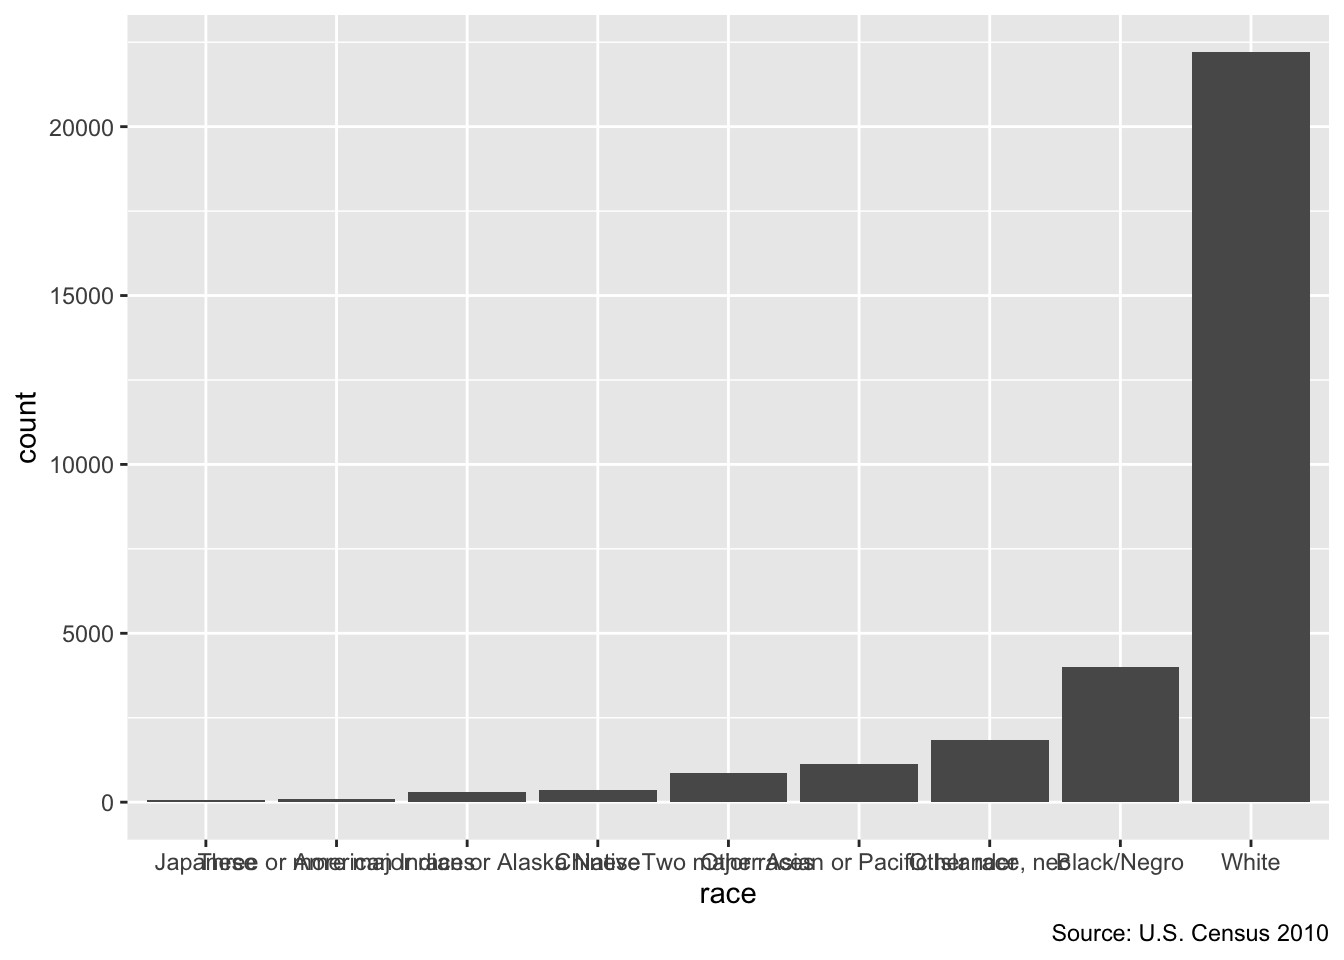
\includegraphics{prefresher_files/figure-latex/unnamed-chunk-210-1.pdf}

You can change the orientation

\begin{Shaded}
\begin{Highlighting}[]
\NormalTok{gg_tab<-}\StringTok{ }\NormalTok{gg_tab }\OperatorTok{+}\StringTok{ }\KeywordTok{coord_flip}\NormalTok{()}
\end{Highlighting}
\end{Shaded}

\hypertarget{parsing-an-object-by-strs}{%
\subsection{\texorpdfstring{Parsing an object by \texttt{str()s}}{Parsing an object by str()s}}\label{parsing-an-object-by-strs}}

It can be hard to understand an \texttt{R} object because it's contents are unknown. The function \texttt{str}, short for structure, is a quick way to look into the innards of an object

\begin{Shaded}
\begin{Highlighting}[]
\KeywordTok{str}\NormalTok{(my_list)}
\end{Highlighting}
\end{Shaded}

\begin{verbatim}
## List of 2
##  $       : chr [1:5] "subitem 1 in slot 1 of my_list" "subitem 1 in slot 2 of my_list" "subitem 1 in slot 3 of my_list" "4" ...
##  $ slot 2: chr "contents of slot named slot 2"
\end{verbatim}

\begin{Shaded}
\begin{Highlighting}[]
\KeywordTok{class}\NormalTok{(my_list)}
\end{Highlighting}
\end{Shaded}

\begin{verbatim}
## [1] "list"
\end{verbatim}

Same for the object we just made

\begin{Shaded}
\begin{Highlighting}[]
\KeywordTok{str}\NormalTok{(pikachu)}
\end{Highlighting}
\end{Shaded}

\begin{verbatim}
## List of 4
##  $ name  : chr "Pikachu"
##  $ number: num 25
##  $ type  : chr "Electric"
##  $ color : chr "Yellow"
##  - attr(*, "class")= chr "Pokemon"
\end{verbatim}

What does a \texttt{ggplot} object look like? Very complicated, but at least you can see it:

\begin{Shaded}
\begin{Highlighting}[]
\CommentTok{# enter this on your console}
\KeywordTok{str}\NormalTok{(gg_tab)}
\end{Highlighting}
\end{Shaded}

\hypertarget{types-of-variables}{%
\section{Types of variables}\label{types-of-variables}}

In the social science we often analyze variables. As you saw in the tutorial, different types of variables require different care.

A key link with what we just learned is that variables are also types of R objects.

\hypertarget{scalars}{%
\subsection{scalars}\label{scalars}}

One number. How many people did we count in our Census sample?

\begin{Shaded}
\begin{Highlighting}[]
\KeywordTok{nrow}\NormalTok{(cen10)}
\end{Highlighting}
\end{Shaded}

\begin{verbatim}
## [1] 30871
\end{verbatim}

Question: What proportion of our census sample is Native American? This number is also a scalar

\begin{Shaded}
\begin{Highlighting}[]
\CommentTok{# Enter yourself}
\KeywordTok{unique}\NormalTok{(cen10}\OperatorTok{$}\NormalTok{race)}
\end{Highlighting}
\end{Shaded}

\begin{verbatim}
## [1] "White"                            "Black/Negro"                     
## [3] "Other race, nec"                  "American Indian or Alaska Native"
## [5] "Chinese"                          "Other Asian or Pacific Islander" 
## [7] "Two major races"                  "Three or more major races"       
## [9] "Japanese"
\end{verbatim}

\begin{Shaded}
\begin{Highlighting}[]
\KeywordTok{mean}\NormalTok{(cen10}\OperatorTok{$}\NormalTok{race }\OperatorTok{==}\StringTok{ "American Indian or Alaska Native"}\NormalTok{)}
\end{Highlighting}
\end{Shaded}

\begin{verbatim}
## [1] 0.009555894
\end{verbatim}

Hint: you can use the function \texttt{mean()} to calcualte the sample mean. The sample proportion is the mean of a sequence of number, where your event of interest is a 1 (or \texttt{TRUE}) and others are 0 (or \texttt{FALSE}).

\hypertarget{numeric-vectors}{%
\subsection{numeric vectors}\label{numeric-vectors}}

A sequence of numbers.

\begin{Shaded}
\begin{Highlighting}[]
\NormalTok{grp_race_ordered}\OperatorTok{$}\NormalTok{count}
\end{Highlighting}
\end{Shaded}

\begin{verbatim}
## [1]    77    88   295   354   869  1129  1839  4013 22207
\end{verbatim}

\begin{Shaded}
\begin{Highlighting}[]
\KeywordTok{class}\NormalTok{(grp_race_ordered}\OperatorTok{$}\NormalTok{count)}
\end{Highlighting}
\end{Shaded}

\begin{verbatim}
## [1] "integer"
\end{verbatim}

Or even, all the ages of the millions of people in our Census. Here are just the first few numbers of the list.

\begin{Shaded}
\begin{Highlighting}[]
\KeywordTok{head}\NormalTok{(cen10}\OperatorTok{$}\NormalTok{age)}
\end{Highlighting}
\end{Shaded}

\begin{verbatim}
## [1]  8 24 37 12 18 50
\end{verbatim}

\hypertarget{characters-aka-strings}{%
\subsection{characters (aka strings)}\label{characters-aka-strings}}

This can be just one stretch of characters

\begin{Shaded}
\begin{Highlighting}[]
\NormalTok{my_name <-}\StringTok{ "Yon Soo"}
\NormalTok{my_name}
\end{Highlighting}
\end{Shaded}

\begin{verbatim}
## [1] "Yon Soo"
\end{verbatim}

\begin{Shaded}
\begin{Highlighting}[]
\KeywordTok{class}\NormalTok{(my_name)}
\end{Highlighting}
\end{Shaded}

\begin{verbatim}
## [1] "character"
\end{verbatim}

or more characters. Notice here that there's a difference between a vector of individual characters and a length-one object of characters.

\begin{Shaded}
\begin{Highlighting}[]
\NormalTok{my_name_letters <-}\StringTok{ }\KeywordTok{c}\NormalTok{(}\StringTok{"S"}\NormalTok{, }\StringTok{"h"}\NormalTok{, }\StringTok{"i"}\NormalTok{, }\StringTok{"r"}\NormalTok{, }\StringTok{"o"}\NormalTok{)}
\NormalTok{my_name_letters}
\end{Highlighting}
\end{Shaded}

\begin{verbatim}
## [1] "S" "h" "i" "r" "o"
\end{verbatim}

\begin{Shaded}
\begin{Highlighting}[]
\KeywordTok{class}\NormalTok{(my_name_letters)}
\end{Highlighting}
\end{Shaded}

\begin{verbatim}
## [1] "character"
\end{verbatim}

Finally, remember that lower vs.~upper case matters in R!

\begin{Shaded}
\begin{Highlighting}[]
\NormalTok{my_name2 <-}\StringTok{ "shiro"}
\NormalTok{my_name }\OperatorTok{==}\StringTok{ }\NormalTok{my_name2}
\end{Highlighting}
\end{Shaded}

\begin{verbatim}
## [1] FALSE
\end{verbatim}

\hypertarget{what-is-a-function}{%
\section{What is a function?}\label{what-is-a-function}}

Most of what we do in R is executing a function. \texttt{read\_csv()}, \texttt{nrow()}, \texttt{ggplot()} .. pretty much anything with a parentheses is a function. And even things like \texttt{\textless{}-} and \texttt{{[}} are functions as well.

A function is a set of instructions with specified ingredients. It takes an \textbf{input}, then \textbf{manipulates} it -- changes it in some way -- and then returns the manipulated product.

One way to see what a function actually does is to enter it without parentheses.

\begin{Shaded}
\begin{Highlighting}[]
\CommentTok{# enter this on your console}
\NormalTok{table}
\end{Highlighting}
\end{Shaded}

You'll see below that the most basic functions are quite complicated internally.

You'll notice that functions contain other functions. \emph{wrapper} functions are functions that ``wrap around'' existing functions. This sounds redundant, but it's an important feature of programming. If you find yourself repeating a command more than two times, you should make your own function, rather than writing the same type of code.

\hypertarget{write-your-own-function}{%
\subsection{Write your own function}\label{write-your-own-function}}

It's worth remembering the basic structure of a function. You create a new function, call it \texttt{my\_fun} by this:

\begin{Shaded}
\begin{Highlighting}[]
\NormalTok{my_fun <-}\StringTok{ }\ControlFlowTok{function}\NormalTok{() \{}
  
\NormalTok{\}}
\end{Highlighting}
\end{Shaded}

If we wanted to generate a function that computed the number of men in your data, what would that look like?

\begin{Shaded}
\begin{Highlighting}[]
\NormalTok{count_men <-}\StringTok{ }\ControlFlowTok{function}\NormalTok{(data) \{}
  
\NormalTok{  nmen <-}\StringTok{ }\KeywordTok{sum}\NormalTok{(data}\OperatorTok{$}\NormalTok{sex }\OperatorTok{==}\StringTok{ "Male"}\NormalTok{)}
  
  \KeywordTok{return}\NormalTok{(nmen)}
\NormalTok{\}}
\end{Highlighting}
\end{Shaded}

Then all we need to do is feed this function a dataset

\begin{Shaded}
\begin{Highlighting}[]
\KeywordTok{count_men}\NormalTok{(cen10)}
\end{Highlighting}
\end{Shaded}

\begin{verbatim}
## [1] 15220
\end{verbatim}

The point of a function is that you can use it again and again without typing up the set of constituent manipulations. So, what if we wanted to figure out the number of men in California?

\begin{Shaded}
\begin{Highlighting}[]
\KeywordTok{count_men}\NormalTok{(cen10[cen10}\OperatorTok{$}\NormalTok{state }\OperatorTok{==}\StringTok{ "California"}\NormalTok{,])}
\end{Highlighting}
\end{Shaded}

\begin{verbatim}
## [1] 1876
\end{verbatim}

Let's go one step further. What if we want to know the proportion of non-whites in a state, just by entering the name of the state? There's multiple ways to do it, but it could look something like this

\begin{Shaded}
\begin{Highlighting}[]
\NormalTok{nw_in_state <-}\StringTok{ }\ControlFlowTok{function}\NormalTok{(data, state) \{}
  
\NormalTok{  s.subset <-}\StringTok{ }\NormalTok{data[data}\OperatorTok{$}\NormalTok{state }\OperatorTok{==}\StringTok{ }\NormalTok{state,]}
\NormalTok{  total.s <-}\StringTok{ }\KeywordTok{nrow}\NormalTok{(s.subset)}
\NormalTok{  nw.s <-}\StringTok{ }\KeywordTok{sum}\NormalTok{(s.subset}\OperatorTok{$}\NormalTok{race }\OperatorTok{!=}\StringTok{ "White"}\NormalTok{)}
  
\NormalTok{  nw.s }\OperatorTok{/}\StringTok{ }\NormalTok{total.s}
\NormalTok{\}}
\end{Highlighting}
\end{Shaded}

The last line is what gets generated from the function. To be more explicit you can wrap the last line around \texttt{return()}. (as in \texttt{return(nw.s/total.s}). \texttt{return()} is used when you want to break out of a function in the middle of it and not wait till the last line.

Try it on your favorite state!

\begin{Shaded}
\begin{Highlighting}[]
\KeywordTok{nw_in_state}\NormalTok{(cen10, }\StringTok{"Massachusetts"}\NormalTok{)}
\end{Highlighting}
\end{Shaded}

\begin{verbatim}
## [1] 0.2040185
\end{verbatim}

\hypertarget{checkpoint-1}{%
\section*{Checkpoint}\label{checkpoint-1}}
\addcontentsline{toc}{section}{Checkpoint}

\hypertarget{section-14}{%
\subsection*{1}\label{section-14}}
\addcontentsline{toc}{subsection}{1}

Try making your own function, \texttt{average\_age\_in\_state}, that will give you the average age of people in a given state.

\begin{Shaded}
\begin{Highlighting}[]
\CommentTok{# Enter on your own}
\end{Highlighting}
\end{Shaded}

\hypertarget{section-15}{%
\subsection*{2}\label{section-15}}
\addcontentsline{toc}{subsection}{2}

Try making your own function, \texttt{asians\_in\_state}, that will give you the number of \texttt{Chinese}, \texttt{Japanese}, and \texttt{Other\ Asian\ or\ Pacific\ Islander} people in a given state.

\begin{Shaded}
\begin{Highlighting}[]
\CommentTok{# Enter on your own}
\end{Highlighting}
\end{Shaded}

\hypertarget{section-16}{%
\subsection*{3}\label{section-16}}
\addcontentsline{toc}{subsection}{3}

Try making your own function, `top\_10\_oldest\_cities', that will give you the names of cities whose population's average age is top 10 oldest.

\begin{Shaded}
\begin{Highlighting}[]
\CommentTok{# Enter on your own}
\end{Highlighting}
\end{Shaded}

\hypertarget{what-is-a-package}{%
\section{What is a package?}\label{what-is-a-package}}

You can think of a package as a suite of functions that other people have already built for you to make your life easier.

\begin{Shaded}
\begin{Highlighting}[]
\KeywordTok{help}\NormalTok{(}\DataTypeTok{package =} \StringTok{"ggplot2"}\NormalTok{)}
\end{Highlighting}
\end{Shaded}

To use a package, you need to do two things: (1) install it, and then (2) load it.

Installing is a one-time thing

\begin{Shaded}
\begin{Highlighting}[]
\KeywordTok{install.packages}\NormalTok{(}\StringTok{"ggplot2"}\NormalTok{)}
\end{Highlighting}
\end{Shaded}

But you need to load each time you start a R instance. So always keep these commands on a script.

\begin{Shaded}
\begin{Highlighting}[]
\KeywordTok{library}\NormalTok{(ggplot2)}
\end{Highlighting}
\end{Shaded}

In \texttt{rstudio.cloud}, we already installed a set of packages for you. But when you start your own R instance, you need to have installed the package at some point.

\hypertarget{conditionals}{%
\section{Conditionals}\label{conditionals}}

Sometimes, you want to execute a command only under certain conditions. This is done through the almost universal function, \texttt{if()}. Inside the \texttt{if} function we enter a logical statement. The line that is adjacent to, or follows, the \texttt{if()} statement only gets executed if the statement returns \texttt{TRUE}.

For example,

For example,

\begin{Shaded}
\begin{Highlighting}[]
\NormalTok{x <-}\StringTok{ }\DecValTok{5}
\ControlFlowTok{if}\NormalTok{ (x }\OperatorTok{>}\DecValTok{0}\NormalTok{) \{}
  \KeywordTok{print}\NormalTok{(}\StringTok{"positive number"}\NormalTok{)}
\NormalTok{\} }\ControlFlowTok{else} \ControlFlowTok{if}\NormalTok{ (x }\OperatorTok{==}\StringTok{ }\DecValTok{0}\NormalTok{)  \{}
  \KeywordTok{print}\NormalTok{ (}\StringTok{"zero"}\NormalTok{)}
\NormalTok{\} }\ControlFlowTok{else}\NormalTok{ \{}
  \KeywordTok{print}\NormalTok{(}\StringTok{"negative number"}\NormalTok{)}
\NormalTok{\}}
\end{Highlighting}
\end{Shaded}

\begin{verbatim}
## [1] "positive number"
\end{verbatim}

You can wrap that whole things in a function

\begin{Shaded}
\begin{Highlighting}[]
\NormalTok{is_positive <-}\StringTok{ }\ControlFlowTok{function}\NormalTok{(number) \{}
  \ControlFlowTok{if}\NormalTok{ (number }\OperatorTok{>}\DecValTok{0}\NormalTok{) \{}
    \KeywordTok{print}\NormalTok{(}\StringTok{"positive number"}\NormalTok{)}
\NormalTok{  \} }\ControlFlowTok{else} \ControlFlowTok{if}\NormalTok{ (number }\OperatorTok{==}\StringTok{ }\DecValTok{0}\NormalTok{)  \{}
    \KeywordTok{print}\NormalTok{ (}\StringTok{"zero"}\NormalTok{)}
\NormalTok{  \} }\ControlFlowTok{else}\NormalTok{ \{}
    \KeywordTok{print}\NormalTok{(}\StringTok{"negative number"}\NormalTok{)}
\NormalTok{  \}}
\NormalTok{\}}

\KeywordTok{is_positive}\NormalTok{(}\DecValTok{5}\NormalTok{)}
\end{Highlighting}
\end{Shaded}

\begin{verbatim}
## [1] "positive number"
\end{verbatim}

\begin{Shaded}
\begin{Highlighting}[]
\KeywordTok{is_positive}\NormalTok{(}\OperatorTok{-}\DecValTok{3}\NormalTok{)}
\end{Highlighting}
\end{Shaded}

\begin{verbatim}
## [1] "negative number"
\end{verbatim}

\hypertarget{for-loops}{%
\section{For-loops}\label{for-loops}}

Loops repeat the same statement, although the statement can be ``the same'' only in an abstract sense. Use the \texttt{for(x\ in\ X)} syntax to repeat the subsequent command as many times as there are elements in the right-hand object \texttt{X}. Each of these elements will be referred to the left-hand index \texttt{x}

First, come up with a vector.

\begin{Shaded}
\begin{Highlighting}[]
\NormalTok{fruits <-}\StringTok{ }\KeywordTok{c}\NormalTok{(}\StringTok{"apples"}\NormalTok{, }\StringTok{"oranges"}\NormalTok{, }\StringTok{"grapes"}\NormalTok{)}
\end{Highlighting}
\end{Shaded}

Now we use the \texttt{fruits} vector in a \texttt{for} loop.

\begin{Shaded}
\begin{Highlighting}[]
\ControlFlowTok{for}\NormalTok{ (fruit }\ControlFlowTok{in}\NormalTok{ fruits) \{}
  \KeywordTok{print}\NormalTok{(}\KeywordTok{paste}\NormalTok{(}\StringTok{"I love"}\NormalTok{, fruit))}
\NormalTok{\}}
\end{Highlighting}
\end{Shaded}

\begin{verbatim}
## [1] "I love apples"
## [1] "I love oranges"
## [1] "I love grapes"
\end{verbatim}

Here \texttt{for()} and \texttt{in} must be part of any for loop. The right hand side \texttt{fruits} must be a thing that exists. Finally the \texttt{left-hand} side object is ``Pick your favor name.'' It is analogous to how we can index a sum with any letter. \(\sum_{i=1}^{10}i\) and \texttt{sum\_\{j\ =\ 1\}\^{}\{10\}j} are in fact the same thing.

\begin{Shaded}
\begin{Highlighting}[]
\ControlFlowTok{for}\NormalTok{ (i }\ControlFlowTok{in} \DecValTok{1}\OperatorTok{:}\KeywordTok{length}\NormalTok{(fruits)) \{}
  \KeywordTok{print}\NormalTok{(}\KeywordTok{paste}\NormalTok{(}\StringTok{"I love"}\NormalTok{, fruits[i]))}
\NormalTok{\}}
\end{Highlighting}
\end{Shaded}

\begin{verbatim}
## [1] "I love apples"
## [1] "I love oranges"
## [1] "I love grapes"
\end{verbatim}

\begin{Shaded}
\begin{Highlighting}[]
\NormalTok{states_of_interest <-}\StringTok{ }\KeywordTok{c}\NormalTok{(}\StringTok{"California"}\NormalTok{, }\StringTok{"Massachusetts"}\NormalTok{, }\StringTok{"New Hampshire"}\NormalTok{, }\StringTok{"Washington"}\NormalTok{)}

\ControlFlowTok{for}\NormalTok{( state }\ControlFlowTok{in}\NormalTok{ states_of_interest)\{}
\NormalTok{  state_data <-}\StringTok{ }\NormalTok{cen10[cen10}\OperatorTok{$}\NormalTok{state }\OperatorTok{==}\StringTok{ }\NormalTok{state,]}
\NormalTok{  nmen <-}\StringTok{ }\KeywordTok{sum}\NormalTok{(state_data}\OperatorTok{$}\NormalTok{sex }\OperatorTok{==}\StringTok{ "Male"}\NormalTok{)}

\NormalTok{  n <-}\StringTok{ }\KeywordTok{nrow}\NormalTok{(state_data)}
\NormalTok{  men_perc <-}\StringTok{ }\KeywordTok{round}\NormalTok{(}\DecValTok{100}\OperatorTok{*}\NormalTok{(nmen}\OperatorTok{/}\NormalTok{n), }\DataTypeTok{digits=}\DecValTok{2}\NormalTok{)}
  \KeywordTok{print}\NormalTok{(}\KeywordTok{paste}\NormalTok{(}\StringTok{"Percentage of men in"}\NormalTok{,state, }\StringTok{"is"}\NormalTok{, men_perc))}

\NormalTok{\}}
\end{Highlighting}
\end{Shaded}

\begin{verbatim}
## [1] "Percentage of men in California is 49.85"
## [1] "Percentage of men in Massachusetts is 47.6"
## [1] "Percentage of men in New Hampshire is 48.55"
## [1] "Percentage of men in Washington is 48.19"
\end{verbatim}

Instead of printing, you can store the information in a vector

\begin{Shaded}
\begin{Highlighting}[]
\NormalTok{states_of_interest <-}\StringTok{ }\KeywordTok{c}\NormalTok{(}\StringTok{"California"}\NormalTok{, }\StringTok{"Massachusetts"}\NormalTok{, }\StringTok{"New Hampshire"}\NormalTok{, }\StringTok{"Washington"}\NormalTok{)}
\NormalTok{male_percentages <-}\StringTok{ }\KeywordTok{c}\NormalTok{()}
\NormalTok{iter <-}\DecValTok{1} 

\ControlFlowTok{for}\NormalTok{( state }\ControlFlowTok{in}\NormalTok{ states_of_interest)\{}
\NormalTok{  state_data <-}\StringTok{ }\NormalTok{cen10[cen10}\OperatorTok{$}\NormalTok{state }\OperatorTok{==}\StringTok{ }\NormalTok{state,]}
\NormalTok{  nmen <-}\StringTok{ }\KeywordTok{sum}\NormalTok{(state_data}\OperatorTok{$}\NormalTok{sex }\OperatorTok{==}\StringTok{ "Male"}\NormalTok{)}
\NormalTok{  n <-}\StringTok{ }\KeywordTok{nrow}\NormalTok{(state_data)}
\NormalTok{  men_perc <-}\StringTok{ }\KeywordTok{round}\NormalTok{(}\DecValTok{100}\OperatorTok{*}\NormalTok{(nmen}\OperatorTok{/}\NormalTok{n), }\DataTypeTok{digits=}\DecValTok{2}\NormalTok{)}
  
\NormalTok{  male_percentages <-}\StringTok{ }\KeywordTok{c}\NormalTok{(male_percentages, men_perc)}
  \KeywordTok{names}\NormalTok{(male_percentages)[iter] <-}\StringTok{ }\NormalTok{state}
\NormalTok{  iter <-}\StringTok{ }\NormalTok{iter }\OperatorTok{+}\StringTok{ }\DecValTok{1}
\NormalTok{\}}

\NormalTok{male_percentages}
\end{Highlighting}
\end{Shaded}

\begin{verbatim}
##    California Massachusetts New Hampshire    Washington 
##         49.85         47.60         48.55         48.19
\end{verbatim}

\hypertarget{nested-loops}{%
\section{Nested Loops}\label{nested-loops}}

What if I want to calculate the population percentage of a race group for all race groups in states of interest?
You could probably use tidyverse functions to do this, but let's try using loops!

\begin{Shaded}
\begin{Highlighting}[]
\NormalTok{states_of_interest <-}\StringTok{ }\KeywordTok{c}\NormalTok{(}\StringTok{"California"}\NormalTok{, }\StringTok{"Massachusetts"}\NormalTok{, }\StringTok{"New Hampshire"}\NormalTok{, }\StringTok{"Washington"}\NormalTok{)}
\ControlFlowTok{for}\NormalTok{ (state }\ControlFlowTok{in}\NormalTok{ states_of_interest) \{}
  \ControlFlowTok{for}\NormalTok{ (race }\ControlFlowTok{in} \KeywordTok{unique}\NormalTok{(cen10}\OperatorTok{$}\NormalTok{race)) \{}
\NormalTok{    race_state_num <-}\StringTok{ }\KeywordTok{nrow}\NormalTok{(cen10[cen10}\OperatorTok{$}\NormalTok{race }\OperatorTok{==}\StringTok{ }\NormalTok{race }\OperatorTok{&}\StringTok{ }\NormalTok{cen10}\OperatorTok{$}\NormalTok{state }\OperatorTok{==}\StringTok{ }\NormalTok{state, ])}
\NormalTok{    state_pop <-}\StringTok{ }\KeywordTok{nrow}\NormalTok{(cen10[cen10}\OperatorTok{$}\NormalTok{state }\OperatorTok{==}\StringTok{ }\NormalTok{state, ])}
\NormalTok{    race_perc <-}\StringTok{ }\KeywordTok{round}\NormalTok{(}\DecValTok{100}\OperatorTok{*}\NormalTok{(race_state_num}\OperatorTok{/}\NormalTok{(state_pop)), }\DataTypeTok{digits=}\DecValTok{2}\NormalTok{)}
    \KeywordTok{print}\NormalTok{(}\KeywordTok{paste}\NormalTok{(}\StringTok{"Percentage of "}\NormalTok{, race , }\StringTok{"in"}\NormalTok{, state, }\StringTok{"is"}\NormalTok{, race_perc))}
\NormalTok{  \}}
\NormalTok{\}}
\end{Highlighting}
\end{Shaded}

\begin{verbatim}
## [1] "Percentage of  White in California is 57.61"
## [1] "Percentage of  Black/Negro in California is 6.72"
## [1] "Percentage of  Other race, nec in California is 15.55"
## [1] "Percentage of  American Indian or Alaska Native in California is 1.12"
## [1] "Percentage of  Chinese in California is 3.75"
## [1] "Percentage of  Other Asian or Pacific Islander in California is 9.54"
## [1] "Percentage of  Two major races in California is 4.62"
## [1] "Percentage of  Three or more major races in California is 0.37"
## [1] "Percentage of  Japanese in California is 0.72"
## [1] "Percentage of  White in Massachusetts is 79.6"
## [1] "Percentage of  Black/Negro in Massachusetts is 5.87"
## [1] "Percentage of  Other race, nec in Massachusetts is 4.02"
## [1] "Percentage of  American Indian or Alaska Native in Massachusetts is 0.77"
## [1] "Percentage of  Chinese in Massachusetts is 2.32"
## [1] "Percentage of  Other Asian or Pacific Islander in Massachusetts is 4.33"
## [1] "Percentage of  Two major races in Massachusetts is 2.78"
## [1] "Percentage of  Three or more major races in Massachusetts is 0"
## [1] "Percentage of  Japanese in Massachusetts is 0.31"
## [1] "Percentage of  White in New Hampshire is 93.48"
## [1] "Percentage of  Black/Negro in New Hampshire is 0.72"
## [1] "Percentage of  Other race, nec in New Hampshire is 0.72"
## [1] "Percentage of  American Indian or Alaska Native in New Hampshire is 0.72"
## [1] "Percentage of  Chinese in New Hampshire is 0.72"
## [1] "Percentage of  Other Asian or Pacific Islander in New Hampshire is 2.17"
## [1] "Percentage of  Two major races in New Hampshire is 0.72"
## [1] "Percentage of  Three or more major races in New Hampshire is 0"
## [1] "Percentage of  Japanese in New Hampshire is 0.72"
## [1] "Percentage of  White in Washington is 76.05"
## [1] "Percentage of  Black/Negro in Washington is 2.9"
## [1] "Percentage of  Other race, nec in Washington is 5.37"
## [1] "Percentage of  American Indian or Alaska Native in Washington is 2.03"
## [1] "Percentage of  Chinese in Washington is 1.31"
## [1] "Percentage of  Other Asian or Pacific Islander in Washington is 6.68"
## [1] "Percentage of  Two major races in Washington is 4.79"
## [1] "Percentage of  Three or more major races in Washington is 0.29"
## [1] "Percentage of  Japanese in Washington is 0.58"
\end{verbatim}

\hypertarget{exercises-3}{%
\section*{Exercises}\label{exercises-3}}
\addcontentsline{toc}{section}{Exercises}

\hypertarget{exercise-1-counting-cvap}{%
\subsection*{Exercise 1: Counting CVAP}\label{exercise-1-counting-cvap}}
\addcontentsline{toc}{subsection}{Exercise 1: Counting CVAP}

A issue raised in Persily's article is that the full-count U.S. Census does not record whether the residents are citizens of the United States\footnote{Here is that argument of his again, more recently in the popular press. \href{http://www.politico.com/magazine/story/2015/06/the-supreme-courts-big-data-problem-118568}{``The Mysterious Number of American Citizens''. June 2, 2015. \emph{POLITICO}}}. Instead, this question is asked in a survey, the American Community Survey. The two are fundamentally different exercises: the Census counts everyone by definition, a survey samples its data. Load the 1 percent sample of the 2015 ACS (\texttt{acs2015\_1percent.csv}, in the \texttt{input} folder) and give an estimate of the proportion of a state's ACS respondents that are reportedly U.S. citizens.

\begin{Shaded}
\begin{Highlighting}[]
\NormalTok{acs<-}\StringTok{ }\KeywordTok{read_csv}\NormalTok{(}\StringTok{"input/acs2015_1percent.csv"}\NormalTok{, }\DataTypeTok{col_types =} \KeywordTok{cols}\NormalTok{())}
\KeywordTok{set.seed}\NormalTok{(}\DecValTok{02138}\NormalTok{)}
\NormalTok{sample_acs <-}\StringTok{ }\KeywordTok{sample_frac}\NormalTok{(acs, }\FloatTok{0.01}\NormalTok{)}

\CommentTok{# Enter yourself}
\end{Highlighting}
\end{Shaded}

\hypertarget{exercise-2-write-your-own-function}{%
\subsection*{Exercise 2: Write your own function}\label{exercise-2-write-your-own-function}}
\addcontentsline{toc}{subsection}{Exercise 2: Write your own function}

Write your own function that makes some task of data analysis simpler. Ideally, it would be a function that helps you do either of the previous tasks in fewer lines of code. You can use the three lines of code that was provided in exercise 1 to wrap that into another function too!

\begin{Shaded}
\begin{Highlighting}[]
\CommentTok{# Enter yourself}
\end{Highlighting}
\end{Shaded}

\hypertarget{exercise-3-using-loops}{%
\subsection*{Exercise 3: Using Loops}\label{exercise-3-using-loops}}
\addcontentsline{toc}{subsection}{Exercise 3: Using Loops}

Using a loop, create a crosstab of sex and race for each state in the set ``states\_of\_interest''

\begin{Shaded}
\begin{Highlighting}[]
\NormalTok{states_of_interest <-}\StringTok{ }\KeywordTok{c}\NormalTok{(}\StringTok{"California"}\NormalTok{, }\StringTok{"Massachusetts"}\NormalTok{, }\StringTok{"New Hampshire"}\NormalTok{, }\StringTok{"Washington"}\NormalTok{)}
\CommentTok{# Enter yourself}
\end{Highlighting}
\end{Shaded}

\hypertarget{exercise-4-storing-information-derived-within-loops-in-a-global-dataframe}{%
\subsection*{Exercise 4: Storing information derived within loops in a global dataframe}\label{exercise-4-storing-information-derived-within-loops-in-a-global-dataframe}}
\addcontentsline{toc}{subsection}{Exercise 4: Storing information derived within loops in a global dataframe}

Recall the following nested loop

\begin{Shaded}
\begin{Highlighting}[]
\NormalTok{states_of_interest <-}\StringTok{ }\KeywordTok{c}\NormalTok{(}\StringTok{"California"}\NormalTok{, }\StringTok{"Massachusetts"}\NormalTok{, }\StringTok{"New Hampshire"}\NormalTok{, }\StringTok{"Washington"}\NormalTok{)}
\ControlFlowTok{for}\NormalTok{ (state }\ControlFlowTok{in}\NormalTok{ states_of_interest) \{}
  \ControlFlowTok{for}\NormalTok{ (race }\ControlFlowTok{in} \KeywordTok{unique}\NormalTok{(cen10}\OperatorTok{$}\NormalTok{race)) \{}
\NormalTok{    race_state_num <-}\StringTok{ }\KeywordTok{nrow}\NormalTok{(cen10[cen10}\OperatorTok{$}\NormalTok{race }\OperatorTok{==}\StringTok{ }\NormalTok{race }\OperatorTok{&}\StringTok{ }\NormalTok{cen10}\OperatorTok{$}\NormalTok{state }\OperatorTok{==}\StringTok{ }\NormalTok{state, ])}
\NormalTok{    state_pop <-}\StringTok{ }\KeywordTok{nrow}\NormalTok{(cen10[cen10}\OperatorTok{$}\NormalTok{state }\OperatorTok{==}\StringTok{ }\NormalTok{state, ])}
\NormalTok{    race_perc <-}\StringTok{ }\KeywordTok{round}\NormalTok{(}\DecValTok{100}\OperatorTok{*}\NormalTok{(race_state_num}\OperatorTok{/}\NormalTok{(state_pop)), }\DataTypeTok{digits=}\DecValTok{2}\NormalTok{)}
    \KeywordTok{print}\NormalTok{(}\KeywordTok{paste}\NormalTok{(}\StringTok{"Percentage of "}\NormalTok{, race , }\StringTok{"in"}\NormalTok{, state, }\StringTok{"is"}\NormalTok{, race_perc))}
\NormalTok{  \}}
\NormalTok{\}}
\end{Highlighting}
\end{Shaded}

\begin{verbatim}
## [1] "Percentage of  White in California is 57.61"
## [1] "Percentage of  Black/Negro in California is 6.72"
## [1] "Percentage of  Other race, nec in California is 15.55"
## [1] "Percentage of  American Indian or Alaska Native in California is 1.12"
## [1] "Percentage of  Chinese in California is 3.75"
## [1] "Percentage of  Other Asian or Pacific Islander in California is 9.54"
## [1] "Percentage of  Two major races in California is 4.62"
## [1] "Percentage of  Three or more major races in California is 0.37"
## [1] "Percentage of  Japanese in California is 0.72"
## [1] "Percentage of  White in Massachusetts is 79.6"
## [1] "Percentage of  Black/Negro in Massachusetts is 5.87"
## [1] "Percentage of  Other race, nec in Massachusetts is 4.02"
## [1] "Percentage of  American Indian or Alaska Native in Massachusetts is 0.77"
## [1] "Percentage of  Chinese in Massachusetts is 2.32"
## [1] "Percentage of  Other Asian or Pacific Islander in Massachusetts is 4.33"
## [1] "Percentage of  Two major races in Massachusetts is 2.78"
## [1] "Percentage of  Three or more major races in Massachusetts is 0"
## [1] "Percentage of  Japanese in Massachusetts is 0.31"
## [1] "Percentage of  White in New Hampshire is 93.48"
## [1] "Percentage of  Black/Negro in New Hampshire is 0.72"
## [1] "Percentage of  Other race, nec in New Hampshire is 0.72"
## [1] "Percentage of  American Indian or Alaska Native in New Hampshire is 0.72"
## [1] "Percentage of  Chinese in New Hampshire is 0.72"
## [1] "Percentage of  Other Asian or Pacific Islander in New Hampshire is 2.17"
## [1] "Percentage of  Two major races in New Hampshire is 0.72"
## [1] "Percentage of  Three or more major races in New Hampshire is 0"
## [1] "Percentage of  Japanese in New Hampshire is 0.72"
## [1] "Percentage of  White in Washington is 76.05"
## [1] "Percentage of  Black/Negro in Washington is 2.9"
## [1] "Percentage of  Other race, nec in Washington is 5.37"
## [1] "Percentage of  American Indian or Alaska Native in Washington is 2.03"
## [1] "Percentage of  Chinese in Washington is 1.31"
## [1] "Percentage of  Other Asian or Pacific Islander in Washington is 6.68"
## [1] "Percentage of  Two major races in Washington is 4.79"
## [1] "Percentage of  Three or more major races in Washington is 0.29"
## [1] "Percentage of  Japanese in Washington is 0.58"
\end{verbatim}

Instead of printing the percentage of each race in each state, create a dataframe, and store all that information in that dataframe. (Hint: look at how I stored information about male percentage in each state of interest in a vector.)

\hypertarget{dempeace}{%
\chapter[Joins and Merges, Wide and Long]{\texorpdfstring{Joins and Merges, Wide and Long\footnote{Module originally written by Shiro Kuriwaki, Connor Jerzak, and Yon Soo Park}}{Joins and Merges, Wide and Long}}\label{dempeace}}

\hypertarget{where-are-we-where-are-we-headed-4}{%
\section*{Where are we? Where are we headed?}\label{where-are-we-where-are-we-headed-4}}
\addcontentsline{toc}{section}{Where are we? Where are we headed?}

Up till now, you should have covered:

\begin{itemize}
\tightlist
\item
  R basic programming
\item
  Counting.
\item
  Visualization.
\item
  Objects and Classes.
\item
  Matrix algebra in R
\item
  Functions.
\end{itemize}

Today you will work on your own, but feel free to ask a fellow classmate nearby or the instructor. The objective for this session is to get more experience using R, but in the process (a) test a prominent theory in the political science literature and (b) explore related ideas of interest to you.

\hypertarget{motivation-1}{%
\section{Motivation}\label{motivation-1}}

The ``Democratic Peace'' is one of the most widely discussed propositions in political science, covering the fields of International Relations and Comparative Politics, with insights to domestic politics of democracies (e.g.~American Politics). The one-sentence idea is that democracies do not fight with each other. There have been much theoretical debate -- for example in earlier work, \href{https://blackboard.angelo.edu/bbcswebdav/institution/LFA/CSS/Course\%20Material/SEC6302/Readings/Lesson_3/Oneal-Russett.pdf}{Oneal and Russet (1999)} argue that the democratic peace is not due to the hegemony of strong democracies like the U.S. and attempt to distinguish between realist and what they call Kantian propositions (e.g.~democratic governance, international organizations)\footnote{\href{https://blackboard.angelo.edu/bbcswebdav/institution/LFA/CSS/Course\%20Material/SEC6302/Readings/Lesson_3/Oneal-Russett.pdf}{The Kantian Peace: The Pacific Benefits of Democracy, Interdependence, and International Organizations, 1885-1992. \emph{World Politics} 52(1):1-37}}.

An empirical demonstration of the democratic peace is also a good example of a \textbf{Time Series Cross Sectional} (or panel) dataset, where the same units (in this case countries) are observed repeatedly for multiple time periods. Experience in assembling and analyzing a TSCS dataset will prepare you for any future research in this area.

\hypertarget{setting-up}{%
\section{Setting up}\label{setting-up}}

\begin{Shaded}
\begin{Highlighting}[]
\KeywordTok{library}\NormalTok{(dplyr)}
\KeywordTok{library}\NormalTok{(tidyr)}
\KeywordTok{library}\NormalTok{(readr)}
\KeywordTok{library}\NormalTok{(data.table)}
\KeywordTok{library}\NormalTok{(foreach)}
\KeywordTok{library}\NormalTok{(readxl)}
\KeywordTok{library}\NormalTok{(ggplot2)}
\end{Highlighting}
\end{Shaded}

\hypertarget{create-a-project-directory}{%
\section{Create a project directory}\label{create-a-project-directory}}

First start a directory for this project. This can be done manually or through RStudio's Project feature(\texttt{File\ \textgreater{}\ New\ Project...})

Directories is the computer science / programming name for folders. While advice about how to structure your working directories might strike you as petty, we believe that starting from some well-tested guides will go a long way in improving the quality and efficiency of your work.

Chapter 4 of Gentzkow and Shapiro's memo, \href{https://web.stanford.edu/~gentzkow/research/CodeAndData.pdf}{Code and Data for the Social Scientist}{]} provides a good template.

\hypertarget{data-sources}{%
\section{Data Sources}\label{data-sources}}

Most projects you do will start with downloading data from elsewhere. For this task, you'll probably want to track down and download the following:

\begin{itemize}
\tightlist
\item
  \textbf{Correlates of war dataset (COW):} Find and download the Militarized Interstate Disputes (MIDs) data from the Correlates of War website: \url{http://www.correlatesofwar.org/data-sets}. Or a dyad-version on dataverse: \url{https://dataverse.harvard.edu/dataset.xhtml?persistentId=hdl:1902.1/11489}
\item
  \textbf{PRIO Data on Armed Conflict:} Find and download the Uppsala Conflict Data Program (UCDP) and PRIO dyad-year data on armed conflict(\url{https://www.prio.org}) or this link to to the flat csv file (\url{http://ucdp.uu.se/downloads/dyadic/ucdp-dyadic-171.csv}).
\item
  \textbf{Polity:} The Polity data can be downloaded from their website (\url{http://www.systemicpeace.org/inscrdata.html}). Look for the newest version of the time series that has the widest coverage.
\end{itemize}

\hypertarget{example-with-2-datasets}{%
\section{Example with 2 Datasets}\label{example-with-2-datasets}}

Let's read in a sample dataset.

\begin{Shaded}
\begin{Highlighting}[]
\NormalTok{polity <-}\StringTok{ }\KeywordTok{read_csv}\NormalTok{(}\StringTok{"input/sample_polity.csv"}\NormalTok{)}
\NormalTok{mid <-}\StringTok{ }\KeywordTok{read_csv}\NormalTok{(}\StringTok{"input/sample_mid.csv"}\NormalTok{)}
\end{Highlighting}
\end{Shaded}

What does \texttt{polity} look like?

\begin{Shaded}
\begin{Highlighting}[]
\KeywordTok{unique}\NormalTok{(polity}\OperatorTok{$}\NormalTok{country)}
\end{Highlighting}
\end{Shaded}

\begin{verbatim}
## [1] "France"        "Prussia"       "Germany"       "United States"
\end{verbatim}

\begin{Shaded}
\begin{Highlighting}[]
\KeywordTok{ggplot}\NormalTok{(polity, }\KeywordTok{aes}\NormalTok{(}\DataTypeTok{x =}\NormalTok{ year, }\DataTypeTok{y =}\NormalTok{ polity2)) }\OperatorTok{+}
\StringTok{  }\KeywordTok{facet_wrap}\NormalTok{(}\OperatorTok{~}\StringTok{ }\NormalTok{country) }\OperatorTok{+}
\StringTok{  }\KeywordTok{geom_line}\NormalTok{()}
\end{Highlighting}
\end{Shaded}

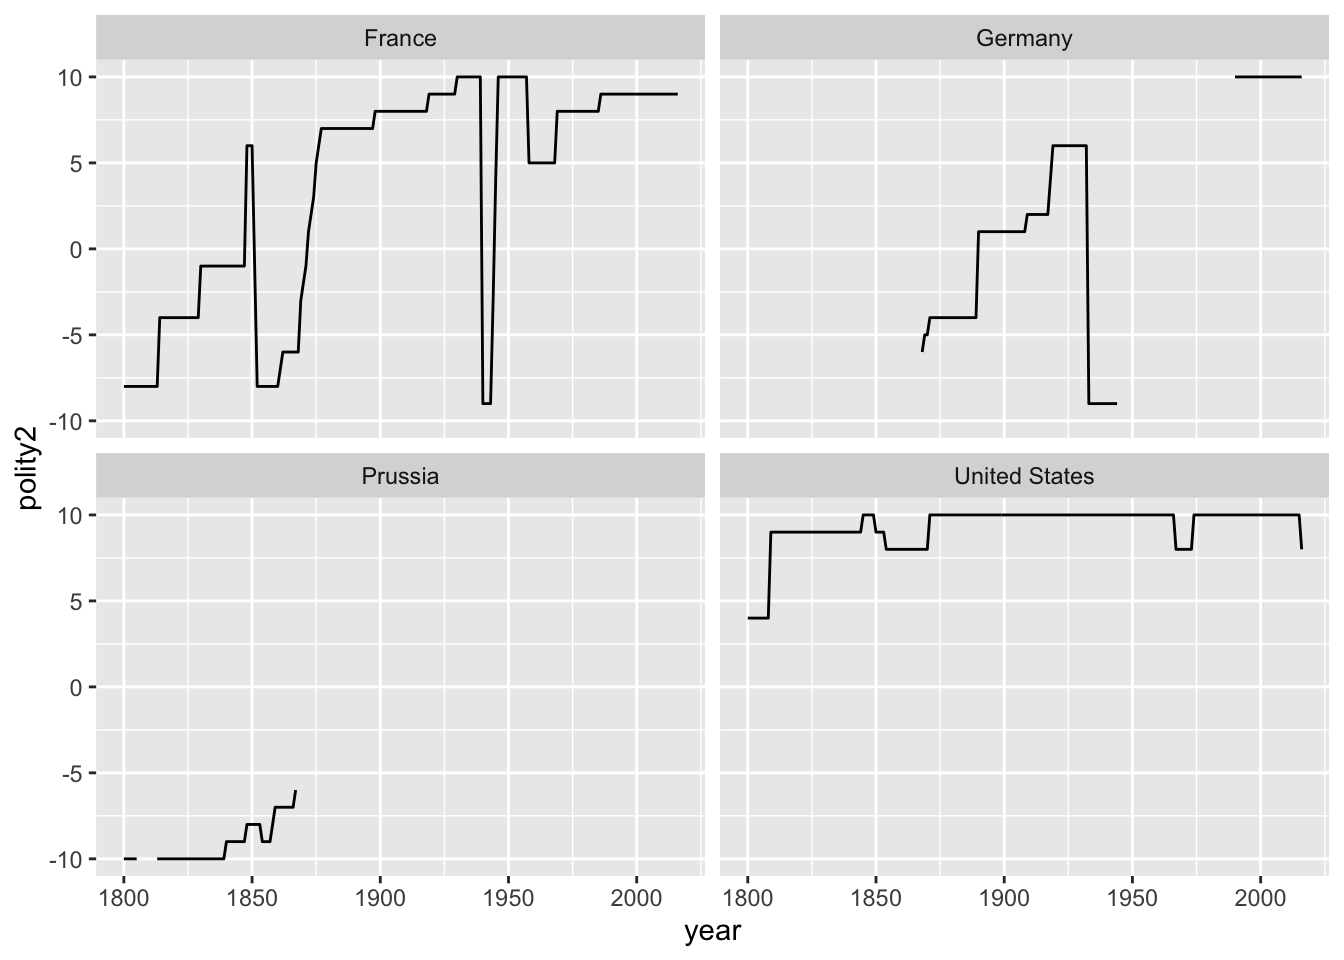
\includegraphics{prefresher_files/figure-latex/unnamed-chunk-250-1.pdf}

\begin{Shaded}
\begin{Highlighting}[]
\KeywordTok{head}\NormalTok{(polity)}
\end{Highlighting}
\end{Shaded}

\begin{verbatim}
## # A tibble: 6 x 5
##   scode ccode country  year polity2
##   <chr> <dbl> <chr>   <dbl>   <dbl>
## 1 FRN     220 France   1800      -8
## 2 FRN     220 France   1801      -8
## 3 FRN     220 France   1802      -8
## 4 FRN     220 France   1803      -8
## 5 FRN     220 France   1804      -8
## 6 FRN     220 France   1805      -8
\end{verbatim}

MID is a dataset that captures a \texttt{dispute} for a given country and year.

\begin{Shaded}
\begin{Highlighting}[]
\NormalTok{mid}
\end{Highlighting}
\end{Shaded}

\begin{verbatim}
## # A tibble: 6,132 x 5
##    ccode polity_code dispute StYear EndYear
##    <dbl> <chr>         <dbl>  <dbl>   <dbl>
##  1   200 UKG               1   1902    1903
##  2     2 USA               1   1902    1903
##  3   345 YGS               1   1913    1913
##  4   300 <NA>              1   1913    1913
##  5   339 ALB               1   1946    1946
##  6   200 UKG               1   1946    1946
##  7   200 UKG               1   1951    1952
##  8   651 EGY               1   1951    1952
##  9   630 IRN               1   1856    1857
## 10   200 UKG               1   1856    1857
## # ... with 6,122 more rows
\end{verbatim}

\hypertarget{loops}{%
\section{Loops}\label{loops}}

Notice that in the \texttt{mid} data, we have a start of a dispute vs.~an end of a dispute.In order to combine this into the \texttt{polity} data, we want a way to give each of the interval years a row.

There are many ways to do this, but one is a loop. We go through one row at a time, and then for each we make a new dataset. that has \texttt{year} as a sequence of each year.

\begin{Shaded}
\begin{Highlighting}[]
\NormalTok{mid_year_by_year <-}\StringTok{ }\KeywordTok{data_frame}\NormalTok{(}\DataTypeTok{ccode =} \KeywordTok{numeric}\NormalTok{(),}
                               \DataTypeTok{year =} \KeywordTok{numeric}\NormalTok{(),}
                               \DataTypeTok{dispute =} \KeywordTok{numeric}\NormalTok{())}

\ControlFlowTok{for}\NormalTok{(i }\ControlFlowTok{in} \DecValTok{1}\OperatorTok{:}\KeywordTok{nrow}\NormalTok{(mid)) \{}
\NormalTok{  x <-}\StringTok{ }\KeywordTok{data_frame}\NormalTok{(}\DataTypeTok{ccode =}\NormalTok{ mid}\OperatorTok{$}\NormalTok{ccode[i], }\CommentTok{## row i's country}
             \DataTypeTok{year =}\NormalTok{ mid}\OperatorTok{$}\NormalTok{StYear[i]}\OperatorTok{:}\NormalTok{mid}\OperatorTok{$}\NormalTok{EndYear[i],  }\CommentTok{## sequence of years for dispute in row i}
             \DataTypeTok{dispute =} \DecValTok{1}\NormalTok{) }
\NormalTok{  mid_year_by_year <-}\StringTok{ }\KeywordTok{rbind}\NormalTok{(mid_year_by_year, x)}
\NormalTok{\}}

\KeywordTok{head}\NormalTok{(mid_year_by_year)}
\end{Highlighting}
\end{Shaded}

\begin{verbatim}
## # A tibble: 6 x 3
##   ccode  year dispute
##   <dbl> <int>   <dbl>
## 1   200  1902       1
## 2   200  1903       1
## 3     2  1902       1
## 4     2  1903       1
## 5   345  1913       1
## 6   300  1913       1
\end{verbatim}

\hypertarget{merging}{%
\section{Merging}\label{merging}}

We want to combine these two datasets by merging. Base-R has a function called \texttt{merge}. \texttt{dplyr} has several types of \texttt{joins} (the same thing). Those names are based on SQL syntax.

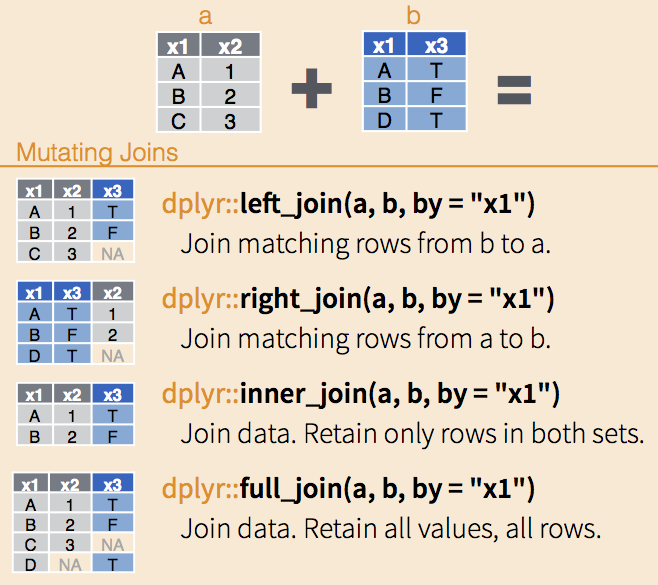
\includegraphics{images/dplyr-joins.png}

Here we can do a \texttt{left\_join} matching rows from \texttt{mid} to \texttt{polity}. We want to keep the rows in \texttt{polity} that do not match in \texttt{mid}, and label them as non-disputes.

\begin{Shaded}
\begin{Highlighting}[]
\NormalTok{p_m <-}\StringTok{ }\KeywordTok{left_join}\NormalTok{(polity,}
                 \KeywordTok{distinct}\NormalTok{(mid_year_by_year),}
                 \DataTypeTok{by =} \KeywordTok{c}\NormalTok{(}\StringTok{"ccode"}\NormalTok{, }\StringTok{"year"}\NormalTok{))}

\KeywordTok{head}\NormalTok{(p_m)}
\end{Highlighting}
\end{Shaded}

\begin{verbatim}
## # A tibble: 6 x 6
##   scode ccode country  year polity2 dispute
##   <chr> <dbl> <chr>   <dbl>   <dbl>   <dbl>
## 1 FRN     220 France   1800      -8      NA
## 2 FRN     220 France   1801      -8      NA
## 3 FRN     220 France   1802      -8      NA
## 4 FRN     220 France   1803      -8      NA
## 5 FRN     220 France   1804      -8      NA
## 6 FRN     220 France   1805      -8      NA
\end{verbatim}

Replace \texttt{dispute} = \texttt{NA} rows with a zero.

\begin{Shaded}
\begin{Highlighting}[]
\NormalTok{p_m}\OperatorTok{$}\NormalTok{dispute[}\KeywordTok{is.na}\NormalTok{(p_m}\OperatorTok{$}\NormalTok{dispute)] <-}\StringTok{ }\DecValTok{0}
\end{Highlighting}
\end{Shaded}

long to wide

\begin{Shaded}
\begin{Highlighting}[]
\NormalTok{p_m_wide <-}\StringTok{ }\KeywordTok{dcast}\NormalTok{(}\DataTypeTok{data =}\NormalTok{ p_m,}
                  \DataTypeTok{formula =}\NormalTok{ ccode }\OperatorTok{~}\StringTok{ }\NormalTok{year,}
                  \DataTypeTok{value.var =} \StringTok{"polity2"}\NormalTok{)}
\end{Highlighting}
\end{Shaded}

\hypertarget{main-project}{%
\section{Main Project}\label{main-project}}

Try building a panel that would be useful in answering the Democratic Peace Question, perhaps in these steps.

\hypertarget{task-1-data-input-and-standardization}{%
\subsection*{Task 1: Data Input and Standardization}\label{task-1-data-input-and-standardization}}
\addcontentsline{toc}{subsection}{Task 1: Data Input and Standardization}

Often, files we need are saved in the \texttt{.xls} or \texttt{xlsx} format. It is possible to read these files directly into \texttt{R}, but experience suggests that this process is slower than converting them first to \texttt{.csv} format and reading them in as \texttt{.csv} files.

\texttt{readxl}/\texttt{readr}/\texttt{haven} packages(\url{https://github.com/tidyverse/tidyverse}) is constantly expanding to capture more file types. In day 1, we used the package \texttt{readxl}, using the \texttt{read\_excel()} function.

\hypertarget{task-2-data-merging}{%
\subsection*{Task 2: Data Merging}\label{task-2-data-merging}}
\addcontentsline{toc}{subsection}{Task 2: Data Merging}

We will use data to test a version of the Democratic Peace Thesis (DPS). Democracies are said to go to war less because the leaders who wage wars are accountable to voters who have to bear the costs of war. Are democracies less likely to engage in militarized interstate disputes?

To start, let's download and merge some data.

\begin{itemize}
\tightlist
\item
  Load in the Militarized Interstate Dispute (MID) files. Militarized interstate disputes are hostile action between two formally recognized states. Examples of this would be threats to use force, threats to declare war, beginning war, fortifying a border with troops, and so on.
\item
  Find a way to \textbf{merge} the Polity IV dataset and the MID data. This process can be a bit tricky.
\item
  An \emph{advanced} version of this task would be to download the dyadic form of the data and try merging that with polity.
\end{itemize}

\hypertarget{task-3-tabulations-and-visualization}{%
\subsection*{Task 3: Tabulations and Visualization}\label{task-3-tabulations-and-visualization}}
\addcontentsline{toc}{subsection}{Task 3: Tabulations and Visualization}

\begin{enumerate}
\def\labelenumi{\arabic{enumi}.}
\tightlist
\item
  Calculate the mean Polity2 score by year. Plot the result. Use graphical indicators of your choosing to show where key events fall in this timeline (such as 1914, 1929, 1939, 1989, 2008). Speculate on why the behavior from 1800 to 1920 seems to be qualitatively different than behavior afterwards.
\item
  Do the same but only among state-years that were invovled in a MID. Plot this line together with your results from 1.
\item
  Do the same but only among state years that were \emph{not} involved in a MID.
\item
  Arrive at a tentative conclusion for how well the Democratic Peace argument seems to hold up in this dataset. Visualize this conclusion.
\end{enumerate}

\hypertarget{simulation}{%
\chapter[Simulation]{\texorpdfstring{Simulation\footnote{Module originally written by Connor Jerzak and Shiro Kuriwaki}}{Simulation}}\label{simulation}}

\hypertarget{where-are-we-where-are-we-headed-5}{%
\subsection*{Where are we? Where are we headed?}\label{where-are-we-where-are-we-headed-5}}
\addcontentsline{toc}{subsection}{Where are we? Where are we headed?}

Up till now, you should have covered:

\begin{itemize}
\tightlist
\item
  \texttt{R} basics
\item
  Visualization
\item
  Matrices and vectors
\item
  Functions, objects, loops
\item
  Joining real data
\end{itemize}

In this module, we will start to work with generating data within R, from thin air, as it were. Doing simulation also strengthens your understanding of Probability (Section @ref\{probability\}).

\hypertarget{check-your-understanding-2}{%
\subsection*{Check your Understanding}\label{check-your-understanding-2}}
\addcontentsline{toc}{subsection}{Check your Understanding}

\begin{itemize}
\tightlist
\item
  What does the \texttt{sample()} function do?
\item
  What does \texttt{runif()} stand for?
\item
  What is a \texttt{seed}?
\item
  What is a Monte Carlo?
\end{itemize}

Check if you have an idea of how you might code the following tasks:

\begin{itemize}
\tightlist
\item
  Simulate 100 rolls of a die
\item
  Simulate one random ordering of 25 numbers
\item
  Simulate 100 values of white noise (uniform random variables)
\item
  Generate a ``bootstrap'' sample of an existing dataset
\end{itemize}

We're going to learn about this today!

\hypertarget{motivation-simulation-as-an-analytical-tool}{%
\section{Motivation: Simulation as an Analytical Tool}\label{motivation-simulation-as-an-analytical-tool}}

An increasing amount of political science contributions now include a simulation.

\begin{itemize}
\tightlist
\item
  \href{http://www-personal.umich.edu/~axe/research/Dissemination.pdf}{Axelrod (1977)} demonstrated via simulation how atomized individuals evolve to be grouped in similar clusters or countries, a model of culture.\footnote{\href{http://www-personal.umich.edu/~axe/research/Dissemination.pdf}{Axelrod, Robert. 1997. ``The Dissemination of Culture.'' \emph{Journal of Conflict Resolution} 41(2): 203--26.}}
\item
  \href{http://www-personal.umich.edu/~jowei/florida.pdf}{Chen and Rodden (2013)} argued in a 2013 article that the vote-seat inequality in U.S. elections that is often attributed to intentional partisan gerrymandering can actually attributed to simply the reality of ``human geography'' -- Democratic voters tend to be concentrated in smaller area. Put another way, no feasible form of gerrymandering could spread out Democratic voters in such a way to equalize their vote-seat translation effectiveness. After demonstrating the empirical pattern of human geography, they advance their key claim by simulating thousands of redistricting plans and record the vote-seat ratio.\footnote{\href{http://www-personal.umich.edu/~jowei/florida.pdf}{Chen, Jowei, and Jonathan Rodden. ``Unintentional Gerrymandering: Political Geography and Electoral Bias in Legislatures. \emph{Quarterly Journal of Political Science}, 8:239-269''}}
\item
  \href{https://gking.harvard.edu/files/abs/evil-abs.shtml}{Gary King, James Honaker, and multiple other authors} propose a way to analyze missing data with a method of multiple imputation, which uses a lot of simulation from a researcher's observed dataset.\footnote{\href{https://gking.harvard.edu/files/abs/evil-abs.shtml}{King, Gary, et al. ``Analyzing Incomplete Political Science Data: An Alternative Algorithm for Multiple Imputation''. \emph{American Political Science Review}, 95: 49-69.}} (Software: Amelia\footnote{\href{http://www.jstatsoft.org/v45/i07/}{James Honaker, Gary King, Matthew Blackwell (2011). Amelia II: A Program for Missing Data. Journal of
    Statistical Software, 45(7), 1-47.}})
\end{itemize}

Statistical methods also incorporate simulation:

\begin{itemize}
\tightlist
\item
  The bootstrap: a statistical method for estimating uncertainty around some parameter by re-sampling observations.
\item
  Bagging: a method for improving machine learning predictions by re-sampling observations, storing the estimate across many re-samples, and averaging these estimates to form the final estimate. A variance reduction technique.
\item
  Statistical reasoning: if you are trying to understand a quantitative problem, a wonderful first-step to understand the problem better is to simulate it! The analytical solution is often very hard (or impossible), but the simulation is often much easier :-)
\end{itemize}

\hypertarget{pick-a-sample-any-sample}{%
\section{Pick a sample, any sample}\label{pick-a-sample-any-sample}}

\hypertarget{the-sample-function}{%
\section{\texorpdfstring{The \texttt{sample()} function}{The sample() function}}\label{the-sample-function}}

The core functions for coding up stochastic data revolves around several key functions, so we will simply review them here.

Suppose you have a vector of values \texttt{x} and from it you want to randomly sample a sample of length \texttt{size}. For this, use the \texttt{sample} function

\begin{Shaded}
\begin{Highlighting}[]
\KeywordTok{sample}\NormalTok{(}\DataTypeTok{x =} \DecValTok{1}\OperatorTok{:}\DecValTok{10}\NormalTok{, }\DataTypeTok{size =} \DecValTok{5}\NormalTok{)}
\end{Highlighting}
\end{Shaded}

\begin{verbatim}
## [1]  3  1  8 10  2
\end{verbatim}

There are two subtypes of sampling -- with and without replacement.

\begin{enumerate}
\def\labelenumi{\arabic{enumi}.}
\tightlist
\item
  Sampling without replacement (\texttt{replace\ =\ FALSE}) means once an element of \texttt{x} is chosen, it will not be considered again:
\end{enumerate}

\begin{Shaded}
\begin{Highlighting}[]
\KeywordTok{sample}\NormalTok{(}\DataTypeTok{x =} \DecValTok{1}\OperatorTok{:}\DecValTok{10}\NormalTok{, }\DataTypeTok{size =} \DecValTok{10}\NormalTok{, }\DataTypeTok{replace =} \OtherTok{FALSE}\NormalTok{) }\CommentTok{## no number appears more than once}
\end{Highlighting}
\end{Shaded}

\begin{verbatim}
##  [1]  4  5  9  2  3  7  1  6 10  8
\end{verbatim}

\begin{enumerate}
\def\labelenumi{\arabic{enumi}.}
\setcounter{enumi}{1}
\tightlist
\item
  Sampling with replacement (\texttt{replace\ =\ TRUE}) means that even if an element of \texttt{x} is chosen, it is put back in the pool and may be chosen again.
\end{enumerate}

\begin{Shaded}
\begin{Highlighting}[]
\KeywordTok{sample}\NormalTok{(}\DataTypeTok{x =} \DecValTok{1}\OperatorTok{:}\DecValTok{10}\NormalTok{, }\DataTypeTok{size =} \DecValTok{10}\NormalTok{, }\DataTypeTok{replace =} \OtherTok{TRUE}\NormalTok{) }\CommentTok{## any number can appear more than once}
\end{Highlighting}
\end{Shaded}

\begin{verbatim}
##  [1] 7 4 9 7 2 2 6 8 6 9
\end{verbatim}

It follows then that you cannot sample without replacement a sample that is larger than the pool.

\begin{Shaded}
\begin{Highlighting}[]
\KeywordTok{sample}\NormalTok{(}\DataTypeTok{x =} \DecValTok{1}\OperatorTok{:}\DecValTok{10}\NormalTok{, }\DataTypeTok{size =} \DecValTok{100}\NormalTok{, }\DataTypeTok{replace =} \OtherTok{FALSE}\NormalTok{)}
\end{Highlighting}
\end{Shaded}

\begin{verbatim}
## Error in sample.int(length(x), size, replace, prob): cannot take a sample larger than the population when 'replace = FALSE'
\end{verbatim}

So far, every element in \texttt{x} has had an equal probability of being chosen. In some application, we want a sampling scheme where some elements are more likely to be chosen than others. The argument \texttt{prob} handles this.

For example, this simulates 20 fair coin tosses (each outcome is equally likely to happen)

\begin{Shaded}
\begin{Highlighting}[]
\KeywordTok{sample}\NormalTok{(}\KeywordTok{c}\NormalTok{(}\StringTok{"Head"}\NormalTok{, }\StringTok{"Tail"}\NormalTok{), }\DataTypeTok{size =} \DecValTok{20}\NormalTok{, }\DataTypeTok{prob =} \KeywordTok{c}\NormalTok{(}\FloatTok{0.5}\NormalTok{, }\FloatTok{0.5}\NormalTok{), }\DataTypeTok{replace =} \OtherTok{TRUE}\NormalTok{)}
\end{Highlighting}
\end{Shaded}

\begin{verbatim}
##  [1] "Tail" "Head" "Tail" "Tail" "Head" "Head" "Tail" "Head" "Head" "Head"
## [11] "Head" "Tail" "Tail" "Tail" "Head" "Head" "Tail" "Tail" "Head" "Tail"
\end{verbatim}

But this simulates 20 biased coin tosses, where say the probability of Tails is 4 times more likely than the number of Heads

\begin{Shaded}
\begin{Highlighting}[]
\KeywordTok{sample}\NormalTok{(}\KeywordTok{c}\NormalTok{(}\StringTok{"Head"}\NormalTok{, }\StringTok{"Tail"}\NormalTok{), }\DataTypeTok{size =} \DecValTok{20}\NormalTok{, }\DataTypeTok{prob =} \KeywordTok{c}\NormalTok{(}\FloatTok{0.2}\NormalTok{, }\FloatTok{0.8}\NormalTok{), }\DataTypeTok{replace =} \OtherTok{TRUE}\NormalTok{)}
\end{Highlighting}
\end{Shaded}

\begin{verbatim}
##  [1] "Tail" "Tail" "Tail" "Head" "Tail" "Tail" "Tail" "Head" "Tail" "Tail"
## [11] "Head" "Tail" "Tail" "Head" "Tail" "Head" "Head" "Head" "Tail" "Head"
\end{verbatim}

\hypertarget{sampling-rows-from-a-dataframe}{%
\subsection{Sampling rows from a dataframe}\label{sampling-rows-from-a-dataframe}}

In tidyverse, there is a convenience function to sample rows randomly: \texttt{sample\_n()} and \texttt{sample\_frac()}.

For example, load the dataset on cars, \texttt{mtcars}, which has 32 observations.

\begin{Shaded}
\begin{Highlighting}[]
\NormalTok{mtcars}
\end{Highlighting}
\end{Shaded}

\begin{verbatim}
##                      mpg cyl  disp  hp drat    wt  qsec vs am gear carb
## Mazda RX4           21.0   6 160.0 110 3.90 2.620 16.46  0  1    4    4
## Mazda RX4 Wag       21.0   6 160.0 110 3.90 2.875 17.02  0  1    4    4
## Datsun 710          22.8   4 108.0  93 3.85 2.320 18.61  1  1    4    1
## Hornet 4 Drive      21.4   6 258.0 110 3.08 3.215 19.44  1  0    3    1
## Hornet Sportabout   18.7   8 360.0 175 3.15 3.440 17.02  0  0    3    2
## Valiant             18.1   6 225.0 105 2.76 3.460 20.22  1  0    3    1
## Duster 360          14.3   8 360.0 245 3.21 3.570 15.84  0  0    3    4
## Merc 240D           24.4   4 146.7  62 3.69 3.190 20.00  1  0    4    2
## Merc 230            22.8   4 140.8  95 3.92 3.150 22.90  1  0    4    2
## Merc 280            19.2   6 167.6 123 3.92 3.440 18.30  1  0    4    4
## Merc 280C           17.8   6 167.6 123 3.92 3.440 18.90  1  0    4    4
## Merc 450SE          16.4   8 275.8 180 3.07 4.070 17.40  0  0    3    3
## Merc 450SL          17.3   8 275.8 180 3.07 3.730 17.60  0  0    3    3
## Merc 450SLC         15.2   8 275.8 180 3.07 3.780 18.00  0  0    3    3
## Cadillac Fleetwood  10.4   8 472.0 205 2.93 5.250 17.98  0  0    3    4
## Lincoln Continental 10.4   8 460.0 215 3.00 5.424 17.82  0  0    3    4
## Chrysler Imperial   14.7   8 440.0 230 3.23 5.345 17.42  0  0    3    4
## Fiat 128            32.4   4  78.7  66 4.08 2.200 19.47  1  1    4    1
## Honda Civic         30.4   4  75.7  52 4.93 1.615 18.52  1  1    4    2
## Toyota Corolla      33.9   4  71.1  65 4.22 1.835 19.90  1  1    4    1
## Toyota Corona       21.5   4 120.1  97 3.70 2.465 20.01  1  0    3    1
## Dodge Challenger    15.5   8 318.0 150 2.76 3.520 16.87  0  0    3    2
## AMC Javelin         15.2   8 304.0 150 3.15 3.435 17.30  0  0    3    2
## Camaro Z28          13.3   8 350.0 245 3.73 3.840 15.41  0  0    3    4
## Pontiac Firebird    19.2   8 400.0 175 3.08 3.845 17.05  0  0    3    2
## Fiat X1-9           27.3   4  79.0  66 4.08 1.935 18.90  1  1    4    1
## Porsche 914-2       26.0   4 120.3  91 4.43 2.140 16.70  0  1    5    2
## Lotus Europa        30.4   4  95.1 113 3.77 1.513 16.90  1  1    5    2
## Ford Pantera L      15.8   8 351.0 264 4.22 3.170 14.50  0  1    5    4
## Ferrari Dino        19.7   6 145.0 175 3.62 2.770 15.50  0  1    5    6
## Maserati Bora       15.0   8 301.0 335 3.54 3.570 14.60  0  1    5    8
## Volvo 142E          21.4   4 121.0 109 4.11 2.780 18.60  1  1    4    2
\end{verbatim}

sample\_n picks a user-specified number of rows from the dataset:

\begin{Shaded}
\begin{Highlighting}[]
\KeywordTok{sample_n}\NormalTok{(mtcars, }\DecValTok{3}\NormalTok{)}
\end{Highlighting}
\end{Shaded}

\begin{verbatim}
##    mpg cyl  disp  hp drat    wt  qsec vs am gear carb
## 1 19.2   8 400.0 175 3.08 3.845 17.05  0  0    3    2
## 2 15.0   8 301.0 335 3.54 3.570 14.60  0  1    5    8
## 3 33.9   4  71.1  65 4.22 1.835 19.90  1  1    4    1
\end{verbatim}

Sometimes you want a X percent sample of your dataset. In this case use \texttt{sample\_frac()}

\begin{Shaded}
\begin{Highlighting}[]
\KeywordTok{sample_frac}\NormalTok{(mtcars, }\FloatTok{0.10}\NormalTok{)}
\end{Highlighting}
\end{Shaded}

\begin{verbatim}
##    mpg cyl  disp  hp drat    wt  qsec vs am gear carb
## 1 15.2   8 304.0 150 3.15 3.435 17.30  0  0    3    2
## 2 16.4   8 275.8 180 3.07 4.070 17.40  0  0    3    3
## 3 14.7   8 440.0 230 3.23 5.345 17.42  0  0    3    4
\end{verbatim}

As a side-note, these functions have very practical uses for any type of data analysis:

\begin{itemize}
\tightlist
\item
  Inspecting your dataset: using \texttt{head()} all the same time and looking over the first few rows might lead you to ignore any issues that end up in the bottom for whatever reason.
\item
  Testing your analysis with a small sample: If running analyses on a dataset takes more than a handful of seconds, change your dataset upstream to a fraction of the size so the rest of the code runs in less than a second. Once verifying your analysis code runs, then re-do it with your full dataset (by simply removing the \texttt{sample\_n} / \texttt{sample\_frac} line of code in the beginning). While three seconds may not sound like much, they accumulate and eat up time.
\end{itemize}

\hypertarget{random-numbers-from-specific-distributions}{%
\section{Random numbers from specific distributions}\label{random-numbers-from-specific-distributions}}

\hypertarget{rbinom}{%
\subsection*{\texorpdfstring{\texttt{rbinom()}}{rbinom()}}\label{rbinom}}
\addcontentsline{toc}{subsection}{\texttt{rbinom()}}

\texttt{rbinom} builds upon \texttt{sample} as a tool to help you answer the question -- what is the \emph{total number of successes} I would get if I sampled a binary (Bernoulli) result from a test with \texttt{size} number of trials each, with a event-wise probability of \texttt{prob}. The first argument \texttt{n} asks me how many such numbers I want.

For example, I want to know how many Heads I would get if I flipped a fair coin 100 times.

\begin{Shaded}
\begin{Highlighting}[]
\KeywordTok{rbinom}\NormalTok{(}\DataTypeTok{n =} \DecValTok{1}\NormalTok{, }\DataTypeTok{size =} \DecValTok{100}\NormalTok{, }\DataTypeTok{prob =} \FloatTok{0.5}\NormalTok{)}
\end{Highlighting}
\end{Shaded}

\begin{verbatim}
## [1] 46
\end{verbatim}

Now imagine this I wanted to do this experiment 10 times, which would require I flip the coin 10 x 100 = 1000 times! Helpfully, we can do this in one line

\begin{Shaded}
\begin{Highlighting}[]
\KeywordTok{rbinom}\NormalTok{(}\DataTypeTok{n =} \DecValTok{10}\NormalTok{, }\DataTypeTok{size =} \DecValTok{100}\NormalTok{, }\DataTypeTok{prob =} \FloatTok{0.5}\NormalTok{)}
\end{Highlighting}
\end{Shaded}

\begin{verbatim}
##  [1] 42 47 41 51 52 57 44 49 53 45
\end{verbatim}

\hypertarget{runif}{%
\subsection*{\texorpdfstring{\texttt{runif()}}{runif()}}\label{runif}}
\addcontentsline{toc}{subsection}{\texttt{runif()}}

\texttt{runif} also simulates a stochastic scheme where each event has equal probability of getting chosen like \texttt{sample}, but is a continuous rather than discrete system. We will cover this more in the next math module.

The intuition to emphasize here is that one can generate potentially infinite amounts (size \texttt{n}) of noise that is a essentially random

\begin{Shaded}
\begin{Highlighting}[]
\KeywordTok{runif}\NormalTok{(}\DataTypeTok{n =} \DecValTok{5}\NormalTok{)}
\end{Highlighting}
\end{Shaded}

\begin{verbatim}
## [1] 0.04820592 0.18489989 0.54155194 0.83747694 0.97833988
\end{verbatim}

\hypertarget{rnorm}{%
\subsection*{\texorpdfstring{\texttt{rnorm()}}{rnorm()}}\label{rnorm}}
\addcontentsline{toc}{subsection}{\texttt{rnorm()}}

\texttt{rnorm} is also a continuous distribution, but draws from a Normal distribution -- perhaps the most important distribution in statistics. It runs the same way as \texttt{runif}

\begin{Shaded}
\begin{Highlighting}[]
\KeywordTok{rnorm}\NormalTok{(}\DataTypeTok{n =} \DecValTok{5}\NormalTok{)}
\end{Highlighting}
\end{Shaded}

\begin{verbatim}
## [1]  0.94704868  0.05728521  0.32914573 -2.90922109  0.08422519
\end{verbatim}

To better visualize the difference between the output of \texttt{runif} and \texttt{rnorm}, let's generate lots of each and plot a histogram.

\begin{Shaded}
\begin{Highlighting}[]
\NormalTok{from_runif <-}\StringTok{ }\KeywordTok{runif}\NormalTok{(}\DataTypeTok{n =} \DecValTok{1000}\NormalTok{)}
\NormalTok{from_rnorm <-}\StringTok{ }\KeywordTok{rnorm}\NormalTok{(}\DataTypeTok{n =} \DecValTok{1000}\NormalTok{)}

\KeywordTok{par}\NormalTok{(}\DataTypeTok{mfrow =} \KeywordTok{c}\NormalTok{(}\DecValTok{1}\NormalTok{, }\DecValTok{2}\NormalTok{)) }\CommentTok{## base-R parameter for two plots at once}
\KeywordTok{hist}\NormalTok{(from_runif)}
\KeywordTok{hist}\NormalTok{(from_rnorm)}
\end{Highlighting}
\end{Shaded}

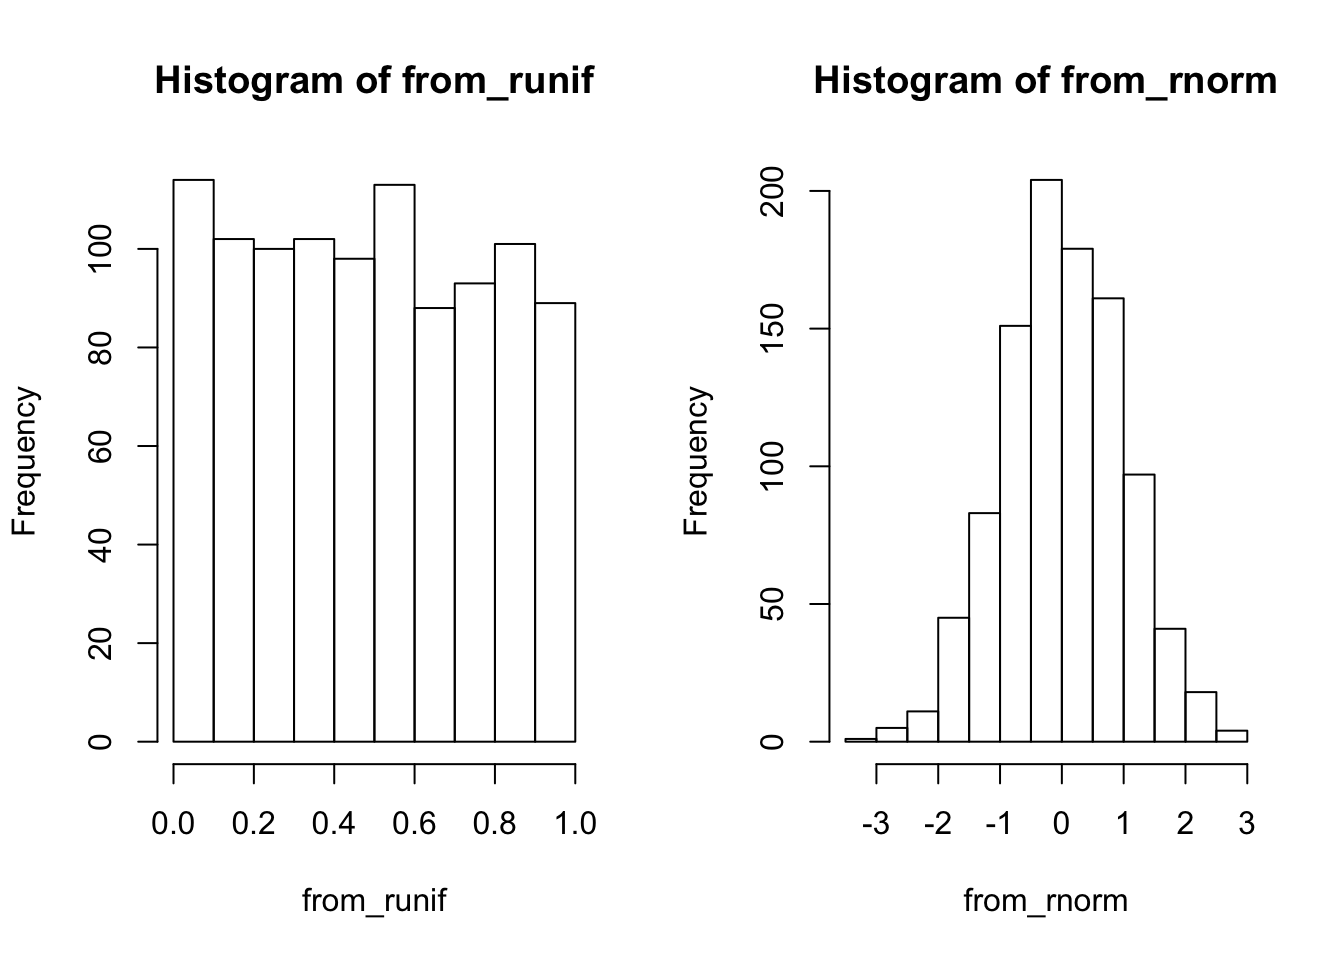
\includegraphics{prefresher_files/figure-latex/unnamed-chunk-273-1.pdf}

\hypertarget{r-p-and-d}{%
\section{r, p, and d}\label{r-p-and-d}}

Each distribution can do more than generate random numbers (the prefix \texttt{r}). We can compute the cumulative probability by the function \texttt{pbinom()}, \texttt{punif()}, and \texttt{pnorm()}. Also the density -- the value of the PDF -- by \texttt{dbinom()}, \texttt{dunif()} and \texttt{dnorm()}.

\hypertarget{set.seed}{%
\section{\texorpdfstring{\texttt{set.seed()}}{set.seed()}}\label{set.seed}}

\texttt{R} doesn't have the ability to generate truly random numbers! Random numbers are actually very hard to generate. (Think: flipping a coin --\textgreater{} can be perfectly predicted if I know wind speed, the angle the coin is flipped, etc.). Some people use random noise in the atmosphere or random behavior in quantum systems to generate ``truly'' (?) random numbers. Conversely, R uses deterministic algorithms which take as an input a ``seed'' and which then perform a series of operations to generate a sequence of random-seeming numbers (that is, numbers whose sequence is sufficiently hard to predict).

Let's think about this another way. Sampling is a stochastic process, so every time you run \texttt{sample()} or \texttt{runif()} you are bound to get a different output (because different random seeds are used). This is intentional in some cases but you might want to avoid it in others. For example, you might want to diagnose a coding discrepancy by setting the random number generator to give the same number each time. To do this, use the function \texttt{set.seed()}.

In the function goes any number. When you run a sample function in the same command as a preceding \texttt{set.seed()}, the sampling function will always give you the same sequence of numbers. In a sense, the sampler is no longer random (in the sense of unpredictable to use; remember: it never was ``truly'' random in the first place)

\begin{Shaded}
\begin{Highlighting}[]
\KeywordTok{set.seed}\NormalTok{(}\DecValTok{02138}\NormalTok{)}
\KeywordTok{runif}\NormalTok{(}\DataTypeTok{n =} \DecValTok{10}\NormalTok{)}
\end{Highlighting}
\end{Shaded}

\begin{verbatim}
##  [1] 0.51236144 0.61530551 0.37451441 0.43541258 0.21166530 0.17812129
##  [7] 0.04420775 0.45567854 0.88718264 0.06970056
\end{verbatim}

The random number generator should give you the exact same sequence of numbers if you precede the function by the same seed,

\begin{Shaded}
\begin{Highlighting}[]
\KeywordTok{set.seed}\NormalTok{(}\DecValTok{02138}\NormalTok{)}
\KeywordTok{runif}\NormalTok{(}\DataTypeTok{n =} \DecValTok{10}\NormalTok{)}
\end{Highlighting}
\end{Shaded}

\begin{verbatim}
##  [1] 0.51236144 0.61530551 0.37451441 0.43541258 0.21166530 0.17812129
##  [7] 0.04420775 0.45567854 0.88718264 0.06970056
\end{verbatim}

whereas a true random number generator would give you the exact same sequence of output with probability 0!

\hypertarget{exercises-4}{%
\section*{Exercises}\label{exercises-4}}
\addcontentsline{toc}{section}{Exercises}

\hypertarget{census-sampling}{%
\subsection*{Census Sampling}\label{census-sampling}}
\addcontentsline{toc}{subsection}{Census Sampling}

What can we learn from surveys of populations, and how wrong do we get if our sampling is biased?\footnote{This example is inspired from \href{https://statistics.fas.harvard.edu/files/statistics-2/files/statistical_paradises_and_paradoxes.pdf}{Meng, Xiao-Li (2018). Statistical paradises and paradoxes in big data (I): Law of large populations, big data paradox, and the 2016 US presidential election. \emph{Annals of Applied Statistics} 12:2, 685--726. doi:10.1214/18-AOAS1161SF.}} Suppose we want to estimate the proportion of U.S. residents who are non-white (\texttt{race\ !=\ "White"}). In reality, we do not have any population dataset to utilize and so we \emph{only see the sample survey}. Here, however, to understand how sampling works, let's conveniently use the Census extract in some cases and pretend we didn't in others.

\begin{enumerate}
\def\labelenumi{(\alph{enumi})}
\item
  First, load \texttt{usc2010\_001percent.csv} into your R session. After loading the \texttt{library(tidyverse)}, browse it. Although this is only a 0.01 percent extract, treat this as your population for pedagogical purposes. What is the population proportion of non-White residents?
\item
  Setting a seed to \texttt{1669482}, sample 100 respondents from this sample. What is the proportion of non-White residents in this \emph{particular} sample? By how many percentage points are you off from (what we labelled as) the true proportion?
\item
  Now imagine what you did above was one survey. What would we get if we did 20 surveys?
\end{enumerate}

To simulate this, write a loop that does the same exercise 20 times, each time computing a sample proportion. Use the same seed at the top, but be careful to position the \texttt{set.seed} function such that it generates the same sequence of 20 samples, rather than 20 of the same sample.

Try doing this with a \texttt{for} loop and storing your sample proportions in a new length-20 vector. (Suggestion: make an empty vector first as a container). After running the loop, show a histogram of the 20 values. Also what is the average of the 20 sample estimates?

\begin{enumerate}
\def\labelenumi{(\alph{enumi})}
\setcounter{enumi}{3}
\tightlist
\item
  Now, to make things more real, let's introduce some response bias. The goal here is not to correct response bias but to induce it and see how it affects our estimates. Suppose that non-White residents are 10 percent less likely to respond to enter your survey than White respondents. This is plausible if you think that the Census is from 2010 but you are polling in 2018, and racial minorities are more geographically mobile than Whites. Repeat the same exercise in (c) by modeling this behavior.
\end{enumerate}

You can do this by creating a variable, e.g. \texttt{propensity}, that is 0.9 for non-Whites and 1 otherwise. Then, you can refer to it in the propensity argument.

\begin{enumerate}
\def\labelenumi{(\alph{enumi})}
\setcounter{enumi}{4}
\item
  Finally, we want to see if more data (``Big Data'') will improve our estimates. Using the same unequal response rates framework as (d), repeat the same exercise but instead of each poll collecting 100 responses, we collect 10,000.
\item
  Optional - visualize your 2 pairs of 20 estimates, with a bar showing the ``correct'' population average.
\end{enumerate}

\hypertarget{conditional-proportions}{%
\subsection*{Conditional Proportions}\label{conditional-proportions}}
\addcontentsline{toc}{subsection}{Conditional Proportions}

This example is not on simulation, but is meant to reinforce some of the probability discussion from math lecture.

Read in the Upshot Siena poll from Fall 2016, \texttt{input/upshot-siena-polls.csv}.

In addition to some standard demographic questions, we will focus on one called \texttt{vt\_pres\_2} in the csv. This is a two-way presidential vote question, asking respondents who they plan to vote for President if the election were held today -- Donald Trump, the Republican, or Hilary Clinton, the Democrat, with options for Other candidates as well. For this problem, use the two-way vote question rather than the 4-way vote question.

\begin{enumerate}
\def\labelenumi{(\alph{enumi})}
\item
  Drop the the respondents who answered the November poll (i.e.~those for which \texttt{poll\ ==\ "November"}). We do this in order to ignore this November population in all subsequent parts of this question because they were not asked the Presidential vote question.
\item
  Using the dataset after the procedure in (a), find the proportion of \emph{poll respondents} (those who are in the sample) who support Donald Trump.
\item
  Among those who supported Donald Trump, what proportion of them has a Bachelor's degree or higher (i.e.~have a Bachelor's, Graduate, or other Professional Degree)?
\item
  Among those who did not support Donald Trump (i.e.~including supporters of Hilary Clinton, another candidate, or those who refused to answer the question), what proportion of them has a Bachelor's degree or higher?
\item
  Express the numbers in the previous parts as probabilities of specified events. Define your own symbols: For example, we can let \(T\) be the event that a randomly selected respondent in the poll supports Donald Trump, then the proportion in part (b) is the probability \(P(T).\)
\item
  Suppose we randomly sampled a person who participated in the survey and found that he/she had a Bachelor's degree or higher. Given this evidence, what is the probability that the same person supports Donald Trump? Use Bayes Rule and show your work -- that is, do not use data or R to compute the quantity directly. Then, verify this is the case via R.
\end{enumerate}

\hypertarget{the-birthday-problem}{%
\subsection*{The Birthday problem}\label{the-birthday-problem}}
\addcontentsline{toc}{subsection}{The Birthday problem}

Write code that will answer the well-known birthday problem via simulation.\footnote{This exercise draws from Imai (2017)}

The problem is fairly simple: Suppose \(k\) people gather together in a room. What is the probability at least two people share the same birthday?

To simplify reality a bit, assume that (1) there are no leap years, and so there are always 365 days in a year, and (2) a given individual's birthday is randomly assigned and independent from each other.

\emph{Step 1}: Set \texttt{k} to a concrete number. Pick a number from 1 to 365 randomly, \texttt{k} times to simulate birthdays (would this be with replacement or without?).

\begin{Shaded}
\begin{Highlighting}[]
\CommentTok{# Your code}
\end{Highlighting}
\end{Shaded}

\emph{Step 2}: Write a line (or two) of code that gives a \texttt{TRUE} or \texttt{FALSE} statement of whether or not at least two people share the same birth date.

\begin{Shaded}
\begin{Highlighting}[]
\CommentTok{# Your code}
\end{Highlighting}
\end{Shaded}

\emph{Step 3}: The above steps will generate a \texttt{TRUE} or \texttt{FALSE} answer for your event of interest, but only for one realization of an event in the sample space. In order to estimate the \emph{probability} of your event happening, we need a ``stochastic'', as opposed to ``deterministic'', method. To do this, write a loop that does Steps 1 and 2 repeatedly for many times, call that number of times \texttt{sims}. For each of \texttt{sims} iteration, your code should give you a \texttt{TRUE} or \texttt{FALSE} answer. Code up a way to store these estimates.

\begin{Shaded}
\begin{Highlighting}[]
\CommentTok{# Your code}
\end{Highlighting}
\end{Shaded}

\emph{Step 4}: Finally, generalize the function further by letting \texttt{k} be a user-defined number. You have now created a \emph{Monte Carlo simulation}!

\begin{Shaded}
\begin{Highlighting}[]
\CommentTok{# Your code}
\end{Highlighting}
\end{Shaded}

\emph{Step 5}: Generate a table or plot that shows how the probability of sharing a birthday changes by \texttt{k} (fixing \texttt{sims} at a large number like \texttt{1000}). Also generate a similar plot that shows how the probability of sharing a birthday changes by \texttt{sims} (fixing \texttt{k} at some arbitrary number like \texttt{10}).

\begin{Shaded}
\begin{Highlighting}[]
\CommentTok{# Your code}
\end{Highlighting}
\end{Shaded}

\emph{Extra credit}: Give an ``analytical'' answer to this problem, that is an answer through deriving the mathematical expressions of the probability.

\begin{Shaded}
\begin{Highlighting}[]
\CommentTok{# Your equations}
\end{Highlighting}
\end{Shaded}

\hypertarget{nonwysiwyg}{%
\chapter[LaTeX and markdown]{\texorpdfstring{LaTeX and markdown\footnote{Module originally written by Shiro Kuriwaki}}{LaTeX and markdown}}\label{nonwysiwyg}}

\hypertarget{where-are-we-where-are-we-headed-6}{%
\subsection*{Where are we? Where are we headed?}\label{where-are-we-where-are-we-headed-6}}
\addcontentsline{toc}{subsection}{Where are we? Where are we headed?}

Up till now, you should have covered:

\begin{itemize}
\tightlist
\item
  Statistical Programming in \texttt{R}
\end{itemize}

This is only the beginning of \texttt{R} -- programming is like learning a language, so learn more as we use it. And yet \texttt{R} is of likely not the only programming language you will want to use. While we cannot introduce everything, we'll pick out a few that we think are particularly helpful.

Here will cover

\begin{itemize}
\tightlist
\item
  Markdown
\item
  LaTeX (and BibTeX)
\end{itemize}

as examples of a non-WYSIWYG editor

and the next chapter (you can read it without reading this LaTeX chapter) covers

\begin{itemize}
\tightlist
\item
  command-line
\item
  git
\end{itemize}

command-line are a basic set of tools that you may have to use from time to time. It also clarifies what more complicated programs are doing. Markdown is an example of compiling a plain text file. LaTeX is a typesetting program and git is a version control program -- both are useful for non-quantitative work as well.

\hypertarget{check-your-understanding-3}{%
\subsection*{Check your understanding}\label{check-your-understanding-3}}
\addcontentsline{toc}{subsection}{Check your understanding}

Check if you have an idea of how you might code the following tasks:

\begin{itemize}
\tightlist
\item
  What does ``WYSIWYG'' stand for? How would a non-WYSIWYG format text?
\item
  How do you start a header in markdown?
\item
  What are some ``plain text'' editors?
\item
  How do you start a document in \texttt{.tex}?
\item
  How do you start a environment in \texttt{.tex}?
\item
  How do you insert a figure in \texttt{.tex}?
\item
  How do you reference a figure in \texttt{.tex}?
\item
  What is a \texttt{.bib} file?
\item
  Say you came across a interesting journal article. How would you want to maintain this reference so that you can refer to its citation in all your subsequent papers?
\end{itemize}

\hypertarget{motivation-2}{%
\section{Motivation}\label{motivation-2}}

Statistical programming is a fast-moving field. The beta version of \texttt{R} was released in 2000, \texttt{ggplot2} was released on 2005, and \texttt{RStudio} started around 2010. Of course, some programming technologies are quite ``old'': (\texttt{C} in 1969, \texttt{C++} around 1989, \texttt{TeX} in 1978, \texttt{Linux} in 1991, Mac OS in 1984). But it is easy to feel you are falling behind in the recent developments of programming. Today we will do a \textbf{brief} and rough overview of some fundamental and new tools other than \texttt{R}, with the general aim of having you break out of your comfort zone so you won't be shut out from learning these tools in the future.

\hypertarget{markdown}{%
\section{Markdown}\label{markdown}}

Markdown is the text we have been using throughout this course! At its core markdown is just plain text. Plain text does not have any formatting embedded in it. Instead, the formatting is coded up as text. Markdown is \emph{not} a WYSIWYG (What you see is what you get) text editor like Microsoft Word or Google Docs. This will mean that you need to explicitly code for \texttt{bold\{text\}} rather than hitting Command+B and making your text look \textbf{bold} on your own computer.

Markdown is known as a ``light-weight'' editor, which means that it is relatively easy to write code that will compile. It is quick and easy and satisfies most presentation purposes; you might want to try \texttt{LaTeX} for more involved papers.

\hypertarget{markdown-commands}{%
\subsection{markdown commands}\label{markdown-commands}}

For italic and bold, use either the asterisks or the underlines,

\begin{verbatim}
*italic*   **bold**
_italic_   __bold__
\end{verbatim}

And for headers use the hash symbols,

\begin{verbatim}
# Main Header
## Sub-headers
\end{verbatim}

\hypertarget{your-own-markdown}{%
\subsection{your own markdown}\label{your-own-markdown}}

RStudio makes it easy to compile your very first markdown file by giving you templates. Got to \texttt{New\ \textgreater{}\ R\ Markdown}, pick a document and click Ok. This will give you a skeleton of a document you can compile -- or ``knit''.

Rmd is actually a slight modification of real markdown. It is a type of file that R reads and turns into a proper \texttt{md} file. Then, it uses a document-conversion called pandoc to compile your \texttt{md} into documents like PDF or HTML.

\begin{figure}
\centering

\includegraphics{images/RMarkdownFlow.png}
\caption{How Rmds become PDFs or HTMLs}
\end{figure}

\hypertarget{a-note-on-plain-text-editors}{%
\subsection{A note on plain-text editors}\label{a-note-on-plain-text-editors}}

Multiple software exist where you can edit plain-text (roughly speaking, text that is not WYSIWYG).

\begin{itemize}
\tightlist
\item
  RStudio (especially for R-related links)
\item
  TeXMaker, TeXShop (especially for TeX)
\item
  \href{https://www.gnu.org/software/emacs/}{emacs}, aquamacs (general)
\item
  \href{http://www.vim.org/download.php}{vim} (general)
\item
  \href{https://www.sublimetext.com}{Sublime Text} (general)
\end{itemize}

Each has their own keyboard shortcuts and special features. You can browse a couple and see which one(s) you like.

\hypertarget{latex}{%
\section{LaTeX}\label{latex}}

LaTeX is a typesetting program. You'd engage with LaTeX much like you engage with your \texttt{R} code. You will interact with LaTeX in a text editor, and will writing code which will be interpreted by the LaTeX compiler and which will finally be parsed to form your final PDF.

\hypertarget{compile-online}{%
\subsection{compile online}\label{compile-online}}

\begin{enumerate}
\def\labelenumi{\arabic{enumi}.}
\tightlist
\item
  Go to \url{https://www.overleaf.com}
\item
  Scroll down and go to ``CREATE A NEW PAPER'' if you don't have an account.
\item
  Let's discuss the default template.
\item
  Make a new document, and set it as your main document. Then type in the Minimal Working Example (MWE):
\end{enumerate}

\begin{Shaded}
\begin{Highlighting}[]
\NormalTok{\textbackslash{}}\ExtensionTok{documentclass}\DataTypeTok{\{article\}}
\NormalTok{\textbackslash{}}\ExtensionTok{begin}\DataTypeTok{\{document\}}
\ExtensionTok{Hello}\NormalTok{ World}
\NormalTok{\textbackslash{}}\ExtensionTok{end}\DataTypeTok{\{document\}}
\end{Highlighting}
\end{Shaded}

\hypertarget{compile-your-first-latex-document-locally}{%
\subsection{compile your first LaTeX document locally}\label{compile-your-first-latex-document-locally}}

LaTeX is a very stable system, and few changes to it have been made since the 1990s. The main benefit: better control over how your papers will look; better methods for writing equations or making tables; overall pleasing aesthetic.

\begin{enumerate}
\def\labelenumi{\arabic{enumi}.}
\tightlist
\item
  Open a plain text editor. Then type in the MWE
\end{enumerate}

\begin{Shaded}
\begin{Highlighting}[]
\NormalTok{\textbackslash{}}\ExtensionTok{documentclass}\DataTypeTok{\{article\}}
\NormalTok{\textbackslash{}}\ExtensionTok{begin}\DataTypeTok{\{document\}}
\ExtensionTok{Hello}\NormalTok{ World}
\NormalTok{\textbackslash{}}\ExtensionTok{end}\DataTypeTok{\{document\}}
\end{Highlighting}
\end{Shaded}

\begin{enumerate}
\def\labelenumi{\arabic{enumi}.}
\setcounter{enumi}{1}
\tightlist
\item
  Save this as \texttt{hello\_world.tex}. Make sure you get the file extension right.
\item
  Open this in your ``LaTeX'' editor. This can be \texttt{TeXMaker}, \texttt{Aqumacs}, etc..
\item
  Go through the click/dropdown interface and click compile.
\end{enumerate}

\hypertarget{main-latex-commands}{%
\subsection{main LaTeX commands}\label{main-latex-commands}}

LaTeX can cover most of your typesetting needs, to clean equations and intricate diagrams.

Some main commands you'll be using are below, and a very concise cheat sheet here: \url{https://wch.github.io/latexsheet/latexsheet.pdf}

Most involved features require that you begin a specific ``environment'' for that feature, clearly demarcating them by the notation \texttt{\textbackslash{}begin\{figure\}} and then \texttt{\textbackslash{}end\{figure\}}, e.g.~in the case of figures.

\begin{verbatim}
\begin{figure}
\includegraphics{histogram.pdf}
\end{figure}
\end{verbatim}

where \texttt{histogram.pdf} is a path to one of your files.

Notice that each line starts with a backslash \texttt{\textbackslash{}} -- in LaTeX this is the symbol to run a command.

The following syntax at the endpoints are shorthand for math equations.

\begin{verbatim}
\[\int x^2 dx\]
\end{verbatim}

these compile math symbols: \(\displaystyle \int x^2 dx.\)\footnote{Enclosing with \texttt{\$\$} instead of \texttt{\textbackslash{}{[}} also has the same effect, so you may see it too. But this is now discouraged due to its inflexibility.}

The \texttt{align} environment is useful to align your multi-line math, for example.

\begin{verbatim}
\begin{align}
P(A \mid B) &= \frac{P(A \cap B)}{P(B)}\\
&= \frac{P(B \mid A)P(A)}{P(B)}
\end{align}
\end{verbatim}

\begin{align}
P(A \mid B) &= \frac{P(A \cap B)}{P(B)}\\
&= \frac{P(B \mid A)P(A)}{P(B)}
\end{align}

Regression tables should be outputted as \texttt{.tex} files with packages like \texttt{xtable} and \texttt{stargazer}, and then called into LaTeX by \texttt{\textbackslash{}input\{regression\_table.tex\}} where \texttt{regression\_table.tex} is the path to your regression output.

Figures and equations should be labelled with the tag (e.g. \texttt{label\{tab:regression\}} so that you can refer to them later with their tag \texttt{Table\ \textbackslash{}ref\{tab:regression\}}, instead of hard-coding \texttt{Table\ 2}).

For some LaTeX commands you might need to load a separate package that someone else has written. Do this in your preamble (i.e.~before \texttt{\textbackslash{}begin\{document\}}):

\begin{verbatim}
\usepackage[options]{package}
\end{verbatim}

where \texttt{package} is the name of the package and \texttt{options} are options specific to the package.

\hypertarget{further-guides}{%
\subsection*{Further Guides}\label{further-guides}}
\addcontentsline{toc}{subsection}{Further Guides}

For a more comprehensive listing of LaTeX commands, Mayya Komisarchik has a great tutorial set of folders: \url{https://scholar.harvard.edu/mkomisarchik/tutorials-0}

There is a version of LaTeX called Beamer, which is a popular way of making a slideshow. Slides in markdown is also a competitor. The language of Beamer is the same as LaTeX but has some special functions for slides.

\hypertarget{bibtex}{%
\section{BibTeX}\label{bibtex}}

BibTeX is a reference system for bibliographical tests. We have a \texttt{.bib} file separately on our computer. This is also a plain text file, but it encodes bibliographical resources with special syntax so that a program can rearrange parts accordingly for different citation systems.

\hypertarget{what-is-a-.bib-file}{%
\subsection{\texorpdfstring{what is a \texttt{.bib} file?}{what is a .bib file?}}\label{what-is-a-.bib-file}}

For example, here is the Nunn and Wantchekon article entry in \texttt{.bib} form.

\begin{verbatim}
@article{nunn2011slave,
  title={The Slave Trade and the Origins of Mistrust in Africa},
  author={Nunn, Nathan and Wantchekon, Leonard},
  journal={American Economic Review},
  volume={101},
  number={7},
  pages={3221--3252},
  year={2011}
}
\end{verbatim}

The first entry, \texttt{nunn2011slave}, is ``pick your favorite'' -- pick your own name for your reference system. The other slots in this \texttt{@article} entry are entries that refer to specific bibliographical text.

\hypertarget{what-does-latex-do-with-.bib-files}{%
\subsection{what does LaTeX do with .bib files?}\label{what-does-latex-do-with-.bib-files}}

Now, in LaTeX, if you type

\begin{verbatim}
  \textcite{nunn2011slave} argue that current variation in the trust among citizens of African countries has historical roots in the European slave trade in the 1600s.
  
\end{verbatim}

as part of your text, then when the \texttt{.tex} file is compiled the PDF shows something like

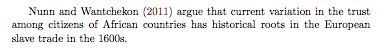
\includegraphics{images/biblatex_inline.png}

in whatever citation style (APSA, APA, Chicago) you pre-specified!

Also at the end of your paper you will have a bibliography with entries ordered and formatted in the appropriate citation.


\includegraphics{images/biblatex_bibliography.png}

This is a much less frustrating way of keeping track of your references -- no need to hand-edit formatting the bibliography to conform to citation rules (which biblatex already knows) and no need to update your bibliography as you add and drop references (biblatex will only show entries that are used in the main text).

\hypertarget{stocking-up-on-your-.bib-files}{%
\subsection{stocking up on your .bib files}\label{stocking-up-on-your-.bib-files}}

You should keep your own \texttt{.bib} file that has all your bibliographical resources. Storing entries is cheap (does not take much memory), so it is fine to keep all your references in one place (but you'll want to make a new one for collaborative projects where multiple people will compile a \texttt{.tex} file).

For example, Gary's BibTeX file is here: \url{https://github.com/iqss-research/gkbibtex/blob/master/gk.bib}

Citation management software (Mendeley or Zotero) automatically generates .bib entries from your library of PDFs for you, provided you have the bibliography attributes right.

\hypertarget{exercise}{%
\section*{Exercise}\label{exercise}}
\addcontentsline{toc}{section}{Exercise}

Create a LaTeX document for a hypothetical research paper on your laptop and, once you've verified it compiles into a PDF, come show it to either one of the instructors.

You can also use overleaf if you have preference for a cloud-based system. But don't swallow the built-in templates without understanding or testing them.

Each student will have slightly different substantive interests, so we won't impose much of a standard. But at a minimum, the LaTeX document should have:

\begin{itemize}
\tightlist
\item
  A title, author, date, and abstract
\item
  Sections
\item
  Italics and boldface
\item
  A figure with a caption and in-text reference to it.
\end{itemize}

Depending on your subfield or interests, try to implement some of the following:

\begin{itemize}
\tightlist
\item
  A bibliographical reference drawing from a separate \texttt{.bib} file
\item
  A table
\item
  A math expression
\item
  A different font
\item
  Different page margins
\item
  Different line spacing
\end{itemize}

\hypertarget{concluding-the-prefresher}{%
\section*{Concluding the Prefresher}\label{concluding-the-prefresher}}
\addcontentsline{toc}{section}{Concluding the Prefresher}

Math may not be the perfect tool for every aspiring political scientist, but hopefully it was useful background to have at the least:

Historians think this totally meaningless and nonsensical statistic is the product of an early-modern epistemological shift in which numbers and quantifiable data became revered above other kinds of knowledge as the most useful and credible form of truth https://t.co/wVFyAQGxEv

--- Gina Anne Tam 譚吉娜 (\citet{DGTam86}) May 29, 2018

But we should be aware that too much slant towards math and programming can miss the point:

To be clear, PhD training in Econ (first year) is often a disaster-- like how to prove the Central Limit Theorem (the LeBron James of Statistics) with polar-cooardinates. This is mostly a way to demoralize actual economists and select a bunch of unimaginative math jocks.

--- Amitabh Chandra (\citet{amitabhchandra2}) August 14, 2018

Keep on learning, trying new techniques to improve your work, and learn from others!

What \#rstats tricks did it take you way too long to learn? One of mine is using readRDS and saveRDS instead of repeatedly loading from CSV

--- Emily Riederer (\citet{EmilyRiederer}) August 19, 2017

\hypertarget{your-feedback-matters}{%
\subsection*{Your Feedback Matters}\label{your-feedback-matters}}
\addcontentsline{toc}{subsection}{Your Feedback Matters}

\emph{Please tell us how we can improve the Prefresher}: The Prefresher is a work in progress, with material mainly driven by graduate students. Please tell us how we should change (or not change) each of its elements:

\url{https://harvard.az1.qualtrics.com/jfe/form/SV_esbzN8ZFAOPTqiV}

\hypertarget{rtext}{%
\chapter[Text]{\texorpdfstring{Text\footnote{Module originally written by Connor Jerzak}}{Text}}\label{rtext}}

\hypertarget{where-are-we-where-are-we-headed-7}{%
\section*{Where are we? Where are we headed?}\label{where-are-we-where-are-we-headed-7}}
\addcontentsline{toc}{section}{Where are we? Where are we headed?}

Up till now, you should have covered:

\begin{itemize}
\tightlist
\item
  Loading in data;
\item
  \texttt{R} notation;
\item
  Matrix algebra.
\end{itemize}

\hypertarget{review}{%
\section{Review}\label{review}}

\begin{itemize}
\tightlist
\item
  \texttt{"} and \texttt{\textquotesingle{}} are usually equivalent.
\item
  \texttt{\textless{}-} and \texttt{=} are usually interchangeable\footnote{Only equal signs are allowed to define the values of a functions' argument}. (\texttt{x\ \textless{}-\ 3} is equivalent to \texttt{x\ =\ 3}, although the former is more preferred because it explicitly states the assignment).
\item
  Use \texttt{(} \texttt{)} when you are giving input to a function:
\end{itemize}

\begin{Shaded}
\begin{Highlighting}[]
\CommentTok{# my_results <- FunctionName(FunctionInputs)}
\end{Highlighting}
\end{Shaded}

\begin{verbatim}
note  `c(1,2,3)` is inputting three numbers in the function `c`
\end{verbatim}

\begin{itemize}
\tightlist
\item
  Use \texttt{\{} \texttt{\}} when you are defining a function or writing a \texttt{for} loop:
\end{itemize}

\begin{Shaded}
\begin{Highlighting}[]
\CommentTok{#function }
\NormalTok{MyFunction <-}\StringTok{ }\ControlFlowTok{function}\NormalTok{(InputMatrix)\{ }
\NormalTok{  TempMat <-}\StringTok{ }\NormalTok{InputMatrix}
  \ControlFlowTok{for}\NormalTok{(i }\ControlFlowTok{in} \DecValTok{1}\OperatorTok{:}\DecValTok{5}\NormalTok{)\{}
\NormalTok{    TempMat <-}\StringTok{ }\KeywordTok{t}\NormalTok{(TempMat)  }\OperatorTok\StringTok{ }\NormalTok{TempMat }\OperatorTok{/}\StringTok{ }\DecValTok{10}
\NormalTok{  \} }
  \KeywordTok{return}\NormalTok{( TempMat )}
\NormalTok{\}}
\NormalTok{myMat <-}\StringTok{ }\KeywordTok{matrix}\NormalTok{(}\KeywordTok{rnorm}\NormalTok{(}\DecValTok{100}\OperatorTok{*}\DecValTok{5}\NormalTok{), }\DataTypeTok{nrow =} \DecValTok{100}\NormalTok{, }\DataTypeTok{ncol =} \DecValTok{5}\NormalTok{)}
\KeywordTok{print}\NormalTok{( }\KeywordTok{MyFunction}\NormalTok{(myMat) ) }
\end{Highlighting}
\end{Shaded}

\begin{verbatim}
##           [,1]      [,2]       [,3]       [,4]      [,5]
## [1,]  342.3602  196.1668   856.7638  -732.7517  173.1954
## [2,]  196.1668  515.3176   762.8554  -277.1625  299.6710
## [3,]  856.7638  762.8554  2697.1230 -1868.8323  461.6741
## [4,] -732.7517 -277.1625 -1868.8323  1678.3580 -264.6936
## [5,]  173.1954  299.6710   461.6741  -264.6936  219.0823
\end{verbatim}

\begin{Shaded}
\begin{Highlighting}[]
\CommentTok{# loop }
\NormalTok{x <-}\StringTok{ }\KeywordTok{c}\NormalTok{() }
\ControlFlowTok{for}\NormalTok{(i }\ControlFlowTok{in} \DecValTok{1}\OperatorTok{:}\DecValTok{20}\NormalTok{)\{}
\NormalTok{  x[i] <-}\StringTok{ }\NormalTok{i }
\NormalTok{\}}
\KeywordTok{print}\NormalTok{(x) }
\end{Highlighting}
\end{Shaded}

\begin{verbatim}
##  [1]  1  2  3  4  5  6  7  8  9 10 11 12 13 14 15 16 17 18 19 20
\end{verbatim}

\hypertarget{goals-for-today}{%
\section{Goals for today}\label{goals-for-today}}

Today, we will learn more about using text data. Our objectives are:

\begin{itemize}
\tightlist
\item
  Reading and writing in text in \texttt{R}.
\item
  To learn how to use paste and sprintf;
\item
  To learn how to use regular expressions;
\item
  To learn about other tools for representing + analyzing text in \texttt{R}.
\end{itemize}

\hypertarget{reading-and-writing-text-in-r}{%
\section{Reading and writing text in R}\label{reading-and-writing-text-in-r}}

\begin{itemize}
\tightlist
\item
  To read in a text file, use readLines
\end{itemize}

\begin{verbatim}
readLines("~/Downloads/Carboxylic acid - Wikipedia.html")
\end{verbatim}

\begin{itemize}
\tightlist
\item
  To write a text file, use:
\end{itemize}

\begin{verbatim}
write.table(my_string_vector, "~/mydata.txt", sep="\t") 
\end{verbatim}

\hypertarget{paste-and-sprintf}{%
\section{\texorpdfstring{\texttt{paste()} and \texttt{sprintf()}}{paste() and sprintf()}}\label{paste-and-sprintf}}

paste and sprintf are useful commands in text processing, such as for automatically naming files or automatically performing a series of command over a subset of your data. Table making also will often need these commands.

Paste concatenates vectors together.

\begin{Shaded}
\begin{Highlighting}[]
\CommentTok{#use collapse for inputs of length > 1 }
\NormalTok{my_string <-}\StringTok{ }\KeywordTok{c}\NormalTok{(}\StringTok{"Not"}\NormalTok{, }\StringTok{"one"}\NormalTok{, }\StringTok{"could"}\NormalTok{, }\StringTok{"equal"}\NormalTok{)}
\KeywordTok{paste}\NormalTok{(my_string, }\DataTypeTok{collapse =} \StringTok{" "}\NormalTok{)}
\end{Highlighting}
\end{Shaded}

\begin{verbatim}
## [1] "Not one could equal"
\end{verbatim}

\begin{Shaded}
\begin{Highlighting}[]
\CommentTok{#use sep for inputs of length == 1 }
\KeywordTok{paste}\NormalTok{(}\StringTok{"Not"}\NormalTok{, }\StringTok{"one"}\NormalTok{, }\StringTok{"could"}\NormalTok{, }\StringTok{"equal"}\NormalTok{, }\DataTypeTok{sep =} \StringTok{" "}\NormalTok{)}
\end{Highlighting}
\end{Shaded}

\begin{verbatim}
## [1] "Not one could equal"
\end{verbatim}

For more sophisticated concatenation, use sprintf. This is very useful for automatically making tables.

\begin{Shaded}
\begin{Highlighting}[]
\KeywordTok{sprintf}\NormalTok{(}\StringTok{"Coefficient for %s: %.3f (%.2f)"}\NormalTok{, }\StringTok{"Gender"}\NormalTok{, }\FloatTok{1.52324}\NormalTok{, }\FloatTok{0.03143}\NormalTok{)}
\end{Highlighting}
\end{Shaded}

\begin{verbatim}
## [1] "Coefficient for Gender: 1.523 (0.03)"
\end{verbatim}

\begin{Shaded}
\begin{Highlighting}[]
\CommentTok{#%s is replaced by a character string}
\CommentTok{#%.3f is replaced by a floating point digit with 3 decimal places}
\CommentTok{#%.2f is replaced by a floating point digit with 2 decimal places}
\end{Highlighting}
\end{Shaded}

\hypertarget{regular-expressions}{%
\section{Regular expressions}\label{regular-expressions}}

A regular expression is a special text string for describing a search pattern.
They are most often used in functions for detecting, locating, and replacing desired text in a corpus.

Use cases:

\begin{enumerate}
\def\labelenumi{\arabic{enumi}.}
\tightlist
\item
  TEXT PARSING. E.g. I have 10000 congressional speaches. Find all those which mention Iran.
\item
  WEB SCRAPING. E.g. Parse html code in order to extract research information from an online table.
\item
  CLEANING DATA. E.g. After loading in a dataset, we might need to remove mistakes from the dataset, orsubset the data using regular expression tools.
\end{enumerate}

Example in \texttt{R}. Extract the tweet mentioning Indonesia.

\begin{Shaded}
\begin{Highlighting}[]
\NormalTok{s1 <-}\StringTok{ "If only Bradley's arm was longer. RT"}
\NormalTok{s2 <-}\StringTok{ "Share our love in Indonesia and in the World. RT if you agree."} 
\NormalTok{my_string <-}\StringTok{ }\KeywordTok{c}\NormalTok{(s1, s2)}
\KeywordTok{grepl}\NormalTok{(my_string, }\DataTypeTok{pattern =} \StringTok{"Indonesia"}\NormalTok{)}
\end{Highlighting}
\end{Shaded}

\begin{verbatim}
## [1] FALSE  TRUE
\end{verbatim}

\begin{Shaded}
\begin{Highlighting}[]
\NormalTok{my_string[ }\KeywordTok{grepl}\NormalTok{(my_string, }\DataTypeTok{pattern =} \StringTok{"Indonesia"}\NormalTok{)]}
\end{Highlighting}
\end{Shaded}

\begin{verbatim}
## [1] "Share our love in Indonesia and in the World. RT if you agree."
\end{verbatim}

Key point: Many R commands use regular expressions. See \texttt{?grepl}. Assume that \texttt{x} is a character vector and that \texttt{pattern} is the target pattern. In the earlier example, \texttt{x} could have been something like \texttt{my\_string} and \texttt{pattern} would have been ``\texttt{Indonesia}''. Here are other key uses:

\begin{enumerate}
\def\labelenumi{\arabic{enumi}.}
\item
  DETECT PATTERNS. \texttt{grepl(pattern,\ x)} goes through all the entries of \texttt{x} and returns a string of TRUE and FALSE values of the same size as \texttt{x}. It will return a \texttt{TRUE} whenever that string entry has the target pattern, and \texttt{FALSE} whenever it doesn't.
\item
  REPLACE PATTERNS. \texttt{gsub(pattern,\ x,\ replacement)} goes through all the entries of \texttt{x} replaces the \texttt{pattern} with \texttt{replacement}.
\end{enumerate}

\begin{Shaded}
\begin{Highlighting}[]
\KeywordTok{gsub}\NormalTok{(}\DataTypeTok{x =}\NormalTok{ my_string,}
     \DataTypeTok{pattern =} \StringTok{"o"}\NormalTok{, }
     \DataTypeTok{replacement =} \StringTok{"AAAA"}\NormalTok{)}
\end{Highlighting}
\end{Shaded}

\begin{verbatim}
## [1] "If AAAAnly Bradley's arm was lAAAAnger. RT"                                   
## [2] "Share AAAAur lAAAAve in IndAAAAnesia and in the WAAAArld. RT if yAAAAu agree."
\end{verbatim}

\begin{enumerate}
\def\labelenumi{\arabic{enumi}.}
\setcounter{enumi}{2}
\tightlist
\item
  LOCATE PATTERNS. \texttt{regexpr(pattern,\ text)} goes through each element of the character string. It returns a vector of the same length, with the entries of the vector corresponding to the location of the first pattern match, or a -1 if no match was obtained.
\end{enumerate}

\begin{Shaded}
\begin{Highlighting}[]
\NormalTok{regex_object <-}\StringTok{ }\KeywordTok{regexpr}\NormalTok{(}\DataTypeTok{pattern =} \StringTok{"was"}\NormalTok{,  }\DataTypeTok{text =}\NormalTok{ my_string)}
\KeywordTok{attr}\NormalTok{(regex_object, }\StringTok{"match.length"}\NormalTok{)}
\end{Highlighting}
\end{Shaded}

\begin{verbatim}
## [1]  3 -1
\end{verbatim}

\begin{Shaded}
\begin{Highlighting}[]
\KeywordTok{attr}\NormalTok{(regex_object, }\StringTok{"useBytes"}\NormalTok{)}
\end{Highlighting}
\end{Shaded}

\begin{verbatim}
## [1] TRUE
\end{verbatim}

\begin{Shaded}
\begin{Highlighting}[]
\KeywordTok{regexpr}\NormalTok{(}\DataTypeTok{pattern =} \StringTok{"was"}\NormalTok{, }\DataTypeTok{text =}\NormalTok{ my_string)[}\DecValTok{1}\NormalTok{]}
\end{Highlighting}
\end{Shaded}

\begin{verbatim}
## [1] 23
\end{verbatim}

\begin{Shaded}
\begin{Highlighting}[]
\KeywordTok{regexpr}\NormalTok{(}\DataTypeTok{pattern =} \StringTok{"was"}\NormalTok{, }\DataTypeTok{text =}\NormalTok{ my_string)[}\DecValTok{2}\NormalTok{]}
\end{Highlighting}
\end{Shaded}

\begin{verbatim}
## [1] -1
\end{verbatim}

Seems simple? The problem: the patterns can get pretty complex!

\hypertarget{character-classes}{%
\subsection{Character classes}\label{character-classes}}

Some types of symbols are stand in for some more complex thing, rather than taken literally.

\texttt{{[}{[}:digit:{]}{]}} Matches with all digits.

\texttt{{[}{[}:lower:{]}{]}} Matches with lower case letters.

\texttt{{[}{[}:alpha:{]}{]}} Matches with all alphabetic characters.

\texttt{{[}{[}:punct:{]}{]}} Matches with all punctuation characters.

\texttt{{[}{[}:cntrl:{]}{]}} Matches with ``control'' characters such as \texttt{\textbackslash{}n}, \texttt{\textbackslash{}r}, etc.

Example in \texttt{R}:

\begin{Shaded}
\begin{Highlighting}[]
\NormalTok{my_string <-}\StringTok{ "Do you think that 34% of apples are red?"}
\KeywordTok{gsub}\NormalTok{(my_string, }\DataTypeTok{pattern =} \StringTok{"[[:digit:]]"}\NormalTok{, }\DataTypeTok{replace =}\StringTok{"DIGIT"}\NormalTok{)}
\end{Highlighting}
\end{Shaded}

\begin{verbatim}
## [1] "Do you think that DIGITDIGIT% of apples are red?"
\end{verbatim}

\begin{Shaded}
\begin{Highlighting}[]
\KeywordTok{gsub}\NormalTok{(my_string, }\DataTypeTok{pattern =} \StringTok{"[[:alpha:]]"}\NormalTok{, }\DataTypeTok{replace =}\StringTok{""}\NormalTok{)}
\end{Highlighting}
\end{Shaded}

\begin{verbatim}
## [1] "    34%    ?"
\end{verbatim}

\hypertarget{special-characters.}{%
\subsection{Special Characters.}\label{special-characters.}}

Certain characters (such as \texttt{.,\ *,\ \textbackslash{}}) have special meaning in the regular expressions framework (they are used to form conditional patterns as discussed below). Thus, when we want our pattern to explicitly include those characters as characters, we must ``escape'' them by using \textbackslash{} or encoding them in \textbackslash{}Q\ldots{}\textbackslash{}E.

Example in \texttt{R}:

\begin{Shaded}
\begin{Highlighting}[]
\NormalTok{my_string <-}\StringTok{ "Do *really* think he will win?"}
\KeywordTok{gsub}\NormalTok{(my_string, }\DataTypeTok{pattern =} \StringTok{"}\CharTok{\textbackslash{}\textbackslash{}}\StringTok{*"}\NormalTok{, }\DataTypeTok{replace =}\StringTok{""}\NormalTok{)}
\end{Highlighting}
\end{Shaded}

\begin{verbatim}
## [1] "Do really think he will win?"
\end{verbatim}

\begin{Shaded}
\begin{Highlighting}[]
\NormalTok{my_string <-}\StringTok{ "Now be brave! }\CharTok{\textbackslash{}n}\StringTok{ Dread what comrades say of you here in combat! "}
\KeywordTok{gsub}\NormalTok{(my_string, }\DataTypeTok{pattern =} \StringTok{"}\CharTok{\textbackslash{}\textbackslash{}\textbackslash{}n}\StringTok{"}\NormalTok{, }\DataTypeTok{replace =}\StringTok{""}\NormalTok{) }
\end{Highlighting}
\end{Shaded}

\begin{verbatim}
## [1] "Now be brave!  Dread what comrades say of you here in combat! "
\end{verbatim}

\hypertarget{conditional-patterns}{%
\subsection{Conditional patterns}\label{conditional-patterns}}

\texttt{{[}{]}} The target characters to match are located between the brackets. For example, \texttt{{[}aAbB{]}} will match with the characters \texttt{a,\ A,\ b,\ B}.

\texttt{{[}\^{}...{]}} Matches with everything except the material between the brackets. For example, \texttt{{[}\^{}aAbB{]}} will match with everything but the characters \texttt{a,\ A,\ b,\ B}.

\texttt{(?=)} Lookahead -- match something that IS followed by the pattern.

\texttt{(?!)} Negative lookahead --- match something that is NOT followed by the pattern.

\texttt{(?\textless{}=)} Lookbehind -- match with something that follows the pattern.

\begin{Shaded}
\begin{Highlighting}[]
\NormalTok{my_string <-}\StringTok{ "Do you think that 34%of the 23%of apples are red?"}
\KeywordTok{gsub}\NormalTok{(my_string, }\DataTypeTok{pattern =} \StringTok{"(?<=%)"}\NormalTok{, }\DataTypeTok{replace =} \StringTok{" "}\NormalTok{, }\DataTypeTok{perl =} \OtherTok{TRUE}\NormalTok{)}
\end{Highlighting}
\end{Shaded}

\begin{verbatim}
## [1] "Do you think that 34% of the 23% of apples are red?"
\end{verbatim}

\begin{Shaded}
\begin{Highlighting}[]
\NormalTok{my_string <-}\StringTok{ }\KeywordTok{c}\NormalTok{(}\StringTok{"legislative1_term1.png"}\NormalTok{, }
               \StringTok{"legislative1_term1.pdf"}\NormalTok{,}
               \StringTok{"legislative1_term2.png"}\NormalTok{,}
               \StringTok{"legislative1_term2.pdf"}\NormalTok{,}
               \StringTok{"term2_presidential1.png"}\NormalTok{, }
               \StringTok{"presidential1.png"}\NormalTok{, }
               \StringTok{"presidential1_term2.png"}\NormalTok{,}
               \StringTok{"presidential1_term1.pdf"}\NormalTok{, }
               \StringTok{"presidential1_term2.pdf"}\NormalTok{)}

\KeywordTok{grepl}\NormalTok{(my_string, }\DataTypeTok{pattern =} \StringTok{"^(?!presidential1).*}\CharTok{\textbackslash{}\textbackslash{}}\StringTok{.png"}\NormalTok{, }\DataTypeTok{perl =} \OtherTok{TRUE}\NormalTok{)}
\end{Highlighting}
\end{Shaded}

\begin{verbatim}
## [1]  TRUE FALSE  TRUE FALSE  TRUE FALSE FALSE FALSE FALSE
\end{verbatim}

\begin{itemize}
\tightlist
\item
  Indicates which file names don't start with \texttt{presidential1} but do end in \texttt{.png}
\item
  \texttt{\^{}} indicates that the pattern should start at the beginning of the string.
\item
  \texttt{?!} indicates negative lookahead -- we're looking for any pattern NOT following presidential1 which meets the subsequent conditions. (see below)
\item
  The first \texttt{.} indicates that, following the negative lookahead, there can be any characters and the * says that it doesn't matter how many. Note that we have to escape the . in \texttt{.png}. (by writing \texttt{\textbackslash{}\textbackslash{}.} instead of just \texttt{.})
\end{itemize}

You will have the chance to try out some regular expressions for yourself at the end!

\hypertarget{representing-text}{%
\section{Representing Text}\label{representing-text}}

In courses and research, we often want to analyze text, to extract meaning out of it.
One of the key decisions we need to make is how to represent the text as numbers.
Once the text is represented numerically, we can then apply a host of statistical
and machine learning methods to it. Those methods are discussed more in the Gov methods sequence (Gov 2000-2003). Here's a summary of the decisions you must make:

\begin{enumerate}
\def\labelenumi{\arabic{enumi}.}
\tightlist
\item
  WHICH TEXT TO USE? Which text do I want to analyze? What is my universe of documents?
\item
  HOW TO REPRESENT THE TEXT NUMERICALLY? How do I use numbers to represent different things about the text?
\item
  HOW TO ANALYZE THE NUMERICAL REPRESENTATION? How do I extract meaning out of the numerical representation?
\end{enumerate}

Representing text numerically.

\begin{enumerate}
\def\labelenumi{\arabic{enumi}.}
\tightlist
\item
  Document term matrix. The document term matrix (DTM) is a common method for representing text. The DTM is a matrix. Each row of this matrix corresponds to a document; each column corresponds to a word. It is often useful to look at summary statistics such as the percentage of speaches in which a Democratic lawmaker used the word ``inequality'' compared to a Republican; the DTM would be very helpful for this and other tasks.
\end{enumerate}

\begin{Shaded}
\begin{Highlighting}[]
\NormalTok{doc1 <-}\StringTok{ "Rage---Goddess, sing the rage of Peleus’ son Achilles,}
\StringTok{         murderous, doomed, that cost the Achaeans countless losses,}
\StringTok{         hurling down to the House of Death so many sturdy souls,}
\StringTok{         great fighters’ souls."}
\NormalTok{doc2 <-}\StringTok{ "And fate? No one alive has ever escaped it,}
\StringTok{         neither brave man nor coward, I tell you, }
\StringTok{         it's born with us the day that we are born."}
\NormalTok{doc3 <-}\StringTok{ "Many cities of men he saw and learned their minds,}
\StringTok{         many pains he suffered, heartsick on the open sea,}
\StringTok{         fighting to save his life and bring his comrades home."}
\end{Highlighting}
\end{Shaded}

\begin{Shaded}
\begin{Highlighting}[]
\NormalTok{DocVec <-}\StringTok{ }\KeywordTok{c}\NormalTok{(doc1, doc2, doc3)}
\end{Highlighting}
\end{Shaded}

Now we can use utility functions in the \texttt{tm} package:

\begin{Shaded}
\begin{Highlighting}[]
\KeywordTok{library}\NormalTok{(tm)}
\NormalTok{DocCorpus <-}\StringTok{ }\KeywordTok{Corpus}\NormalTok{(}\KeywordTok{VectorSource}\NormalTok{(DocVec) ) }
\NormalTok{DTM1 <-}\StringTok{  }\KeywordTok{inspect}\NormalTok{( }\KeywordTok{DocumentTermMatrix}\NormalTok{(DocCorpus) ) }
\end{Highlighting}
\end{Shaded}

Consider the effect of different ``pre-processing'' choices on the resulting DTM!

\begin{Shaded}
\begin{Highlighting}[]
\NormalTok{DocVec <-}\StringTok{ }\KeywordTok{tolower}\NormalTok{(DocVec)}
\NormalTok{DocVec <-}\StringTok{ }\KeywordTok{gsub}\NormalTok{(DocVec, }\DataTypeTok{pattern =}\StringTok{"[[:punct:]]"}\NormalTok{, }\DataTypeTok{replace =} \StringTok{" "}\NormalTok{)}
\NormalTok{DocVec <-}\StringTok{ }\KeywordTok{gsub}\NormalTok{(DocVec, }\DataTypeTok{pattern =}\StringTok{"[[:cntrl:]]"}\NormalTok{, }\DataTypeTok{replace =} \StringTok{" "}\NormalTok{)}
\NormalTok{DocCorpus <-}\StringTok{ }\KeywordTok{Corpus}\NormalTok{(}\KeywordTok{VectorSource}\NormalTok{(DocVec) ) }
\NormalTok{DTM2 <-}\StringTok{  }\KeywordTok{inspect}\NormalTok{(}\KeywordTok{DocumentTermMatrix}\NormalTok{(DocCorpus, }
                                    \DataTypeTok{control =} \KeywordTok{list}\NormalTok{(}\DataTypeTok{stopwords =} \OtherTok{TRUE}\NormalTok{,  }\DataTypeTok{stemming =} \OtherTok{TRUE}\NormalTok{))) }
\end{Highlighting}
\end{Shaded}

Stemming is the process of reducing inflected/derived words to their word stem or base (e.g.~stemming, stemmed, stemmer --\textgreater{} stem*)

\hypertarget{important-packages-for-parsing-text}{%
\section{Important packages for parsing text}\label{important-packages-for-parsing-text}}

\begin{enumerate}
\def\labelenumi{\arabic{enumi}.}
\tightlist
\item
  rvest -- Useful for downloading and manipulating HTML and XM.
\item
  tm -- Useful for converting text into a numerical representation (forming DTMs).
\item
  stringr -- Useful for string parsing.
\end{enumerate}

\hypertarget{exercises-5}{%
\section*{Exercises}\label{exercises-5}}
\addcontentsline{toc}{section}{Exercises}

\hypertarget{section-17}{%
\subsection*{1}\label{section-17}}
\addcontentsline{toc}{subsection}{1}

Figure out why this command does what it does:

\begin{Shaded}
\begin{Highlighting}[]
\KeywordTok{sprintf}\NormalTok{(}\StringTok{"%s of spontaneous events are %s in the mind. }
\StringTok{        Really, %.2f?"}\NormalTok{, }
        \StringTok{"15.03322123"}\NormalTok{, }\StringTok{"puzzles"}\NormalTok{, }\FloatTok{15.03322123}\NormalTok{)}
\end{Highlighting}
\end{Shaded}

\begin{verbatim}
## [1] "15.03322123 of spontaneous events are puzzles in the mind. \n        Really, 15.03?"
\end{verbatim}

\hypertarget{section-18}{%
\subsection*{2}\label{section-18}}
\addcontentsline{toc}{subsection}{2}

Why does this command not work?

\begin{Shaded}
\begin{Highlighting}[]
\KeywordTok{try}\NormalTok{(}\KeywordTok{sprintf}\NormalTok{(}\StringTok{"%s of spontaneous events are %s in the mind. Really, %.2f?"}\NormalTok{,}
            \StringTok{"15.03322123"}\NormalTok{, }\StringTok{"puzzles"}\NormalTok{, }\StringTok{"15.03322123"}\NormalTok{ ), }\OtherTok{TRUE}\NormalTok{)  }
\end{Highlighting}
\end{Shaded}

\hypertarget{section-19}{%
\subsection*{3}\label{section-19}}
\addcontentsline{toc}{subsection}{3}

Using \texttt{grepl}, these materials, Google, and your friends, describe what the following command does. What changes when \texttt{value\ =\ FALSE}?

\begin{Shaded}
\begin{Highlighting}[]
\KeywordTok{grep}\NormalTok{(}\StringTok{'}\CharTok{\textbackslash{}'}\StringTok{'}\NormalTok{, }
     \KeywordTok{c}\NormalTok{(}\StringTok{"To dare is to lose one's footing momentarily."}\NormalTok{,  }\StringTok{"To not dare is to lose oneself."}\NormalTok{), }\DataTypeTok{value =} \OtherTok{TRUE}\NormalTok{)}
\end{Highlighting}
\end{Shaded}

\begin{verbatim}
## [1] "To dare is to lose one's footing momentarily."
\end{verbatim}

\hypertarget{section-20}{%
\subsection*{4}\label{section-20}}
\addcontentsline{toc}{subsection}{4}

Write code to automatically extract the file names that DO end start with presidential and DO end in .pdf

\begin{Shaded}
\begin{Highlighting}[]
\NormalTok{my_string <-}\StringTok{ }\KeywordTok{c}\NormalTok{(}\StringTok{"legislative1_term1.png"}\NormalTok{, }
               \StringTok{"legislative1_term1.pdf"}\NormalTok{,}
               \StringTok{"legislative1_term2.png"}\NormalTok{, }
               \StringTok{"legislative1_term2.pdf"}\NormalTok{,}
               \StringTok{"term2_presidential1.png"}\NormalTok{, }
               \StringTok{"presidential1.png"}\NormalTok{, }
               \StringTok{"presidential1_term2.png"}\NormalTok{,}
               \StringTok{"presidential1_term1.pdf"}\NormalTok{,}
               \StringTok{"presidential1_term2.pdf"}\NormalTok{)}
\end{Highlighting}
\end{Shaded}

\hypertarget{section-21}{%
\subsection*{5}\label{section-21}}
\addcontentsline{toc}{subsection}{5}

Using the same string as in the above, write code to automatically extract the file names that end in .pdf and that contain the text \texttt{term2}.

\begin{Shaded}
\begin{Highlighting}[]
\CommentTok{# Your code here}
\end{Highlighting}
\end{Shaded}

\hypertarget{section-22}{%
\subsection*{6}\label{section-22}}
\addcontentsline{toc}{subsection}{6}

Combine these two strings into a single string separated by a ``-''. Desired output: ``The carbonyl group in aldehydes and ketones is an oxygen analog of the carbon--carbon double bond.''

\begin{Shaded}
\begin{Highlighting}[]
\NormalTok{string1 <-}\StringTok{ "The carbonyl group in aldehydes and ketones }
\StringTok{            is an oxygen analog of the carbon"} 
\NormalTok{string2 <-}\StringTok{  "–carbon double bond."}
\end{Highlighting}
\end{Shaded}

\hypertarget{section-23}{%
\subsection*{7}\label{section-23}}
\addcontentsline{toc}{subsection}{7}

Challenge problem! Download this webpage \url{https://en.wikipedia.org/wiki/Odyssey}

\begin{itemize}
\tightlist
\item
  Read the html file into your R workspace.
\item
  Remove all of the htlm tags (you may need Google to help with this one).
\item
  Remove all punctuation.
\item
  Make all the characters lower case.
\item
  Do this same process with this webpage (\url{https://en.wikipedia.org/wiki/Iliad}).
\item
  Form a document term matrix from the two resulting text strings.
\end{itemize}

\begin{Shaded}
\begin{Highlighting}[]
\CommentTok{# Your code here}
\end{Highlighting}
\end{Shaded}

\hypertarget{commandline-git}{%
\chapter[Command-line, git]{\texorpdfstring{Command-line, git\footnote{Module originally written by Shiro Kuriwaki}}{Command-line, git}}\label{commandline-git}}

\hypertarget{where-are-we-where-are-we-headed-8}{%
\section{Where are we? Where are we headed?}\label{where-are-we-where-are-we-headed-8}}

Up till now, you should have covered:

\begin{itemize}
\tightlist
\item
  Statistical Programming in \texttt{R}
\end{itemize}

In conjunction with the markdown/LaTeX chapter, which is mostly used for typesetting and presentation, here we'll introduce the command-line and git, more used for software extensions and version control

\hypertarget{check-your-understanding-4}{%
\section{Check your understanding}\label{check-your-understanding-4}}

Check if you have an idea of how you might code the following tasks:

\begin{itemize}
\tightlist
\item
  What is a GUI?
\item
  What do the following commands stand for in shell: \texttt{ls} (or \texttt{dir} in Windows), \texttt{cd}, \texttt{rm}, \texttt{mv} (or \texttt{move} in windows), \texttt{cp} (or \texttt{copy} in Windows).
\item
  What is the difference between a relative path and an absolute path?
\item
  What paths do these refer to in shell/terminal: \texttt{\textasciitilde{}/}, \texttt{.}, \texttt{..}
\item
  What is a \emph{repository} in github?
\item
  What does it mean to ``clone'' a repository?
\end{itemize}

\hypertarget{command-line}{%
\section{command-line}\label{command-line}}

Elementary programming operations are done on the command-line, or by entering commands into your computer. This is different from a UI or GUI -- graphical user-interface -- which are interfaces that allow you to click buttons and enter commands in more readable form. Although there are good enough GUIs for most of your needs, you still might need to go under the hood sometimes and run a command.

\hypertarget{command-line-commands}{%
\subsection{command-line commands}\label{command-line-commands}}

Open up \texttt{Terminal} in a Mac. (\texttt{Command\ Prompt} in Windows)

Running this command in a Mac (\texttt{dir} in Windows) should show you a list of all files in the directory that you are currently in.

\begin{Shaded}
\begin{Highlighting}[]
\FunctionTok{ls}
\end{Highlighting}
\end{Shaded}

\begin{verbatim}
## 01_warmup.Rmd
## 02_linear-algebra.Rmd
## 03_functions.Rmd
## 04_limits.Rmd
## 05_calculus.Rmd
## 06_optimization.Rmd
## 07_probability.Rmd
## 11_data-handling_counting.Rmd
## 12_matricies-manipulation.Rmd
## 13_visualization.Rmd
## 14_functions_obj_loops.Rmd
## 15_project-dempeace.Rmd
## 16_simulation.Rmd
## 17_non-wysiwyg.Rmd
## 18_text.Rmd
## 19_command-line_git.Rmd
## 21_solutions-warmup.Rmd
## 23_solution_programming.Rmd
## CODE_OF_CONDUCT.md
## CONTRIBUTING.md
## LICENSE
## README.md
## _book
## _bookdown.yml
## _bookdown_files
## _output.yml
## book.bib
## images
## index.Rmd
## input
## math-prefresher-text.html
## preamble.tex
## prefresher.Rmd
## prefresher.Rproj
## prefresher.bbl
## prefresher.blg
## prefresher.log
## prefresher.pdf
## prefresher.tex
## prefresher_files
## rsconnect
## sample_library.bib
## style.css
\end{verbatim}

\texttt{pwd} stands for present working directory (\texttt{cd} in Windows)

\begin{Shaded}
\begin{Highlighting}[]
\BuiltInTok{pwd}
\end{Highlighting}
\end{Shaded}

\begin{verbatim}
## /Users/shirokuriwaki/Dropbox/prefresher
\end{verbatim}

\texttt{cd} means change directory. You need to give it what to change your current directory \emph{to}. You can specify a name of another directory in your directory.

Or you can go up to your parent directory. The syntax for that are two periods, \texttt{..} . One period \texttt{.} refers to the current directory.

\begin{Shaded}
\begin{Highlighting}[]
\BuiltInTok{cd}\NormalTok{ ..}
\BuiltInTok{pwd}
\end{Highlighting}
\end{Shaded}

\begin{verbatim}
## /Users/shirokuriwaki/Dropbox
\end{verbatim}

\texttt{\textasciitilde{}/} stands for your home directory defined by your computer.

\begin{Shaded}
\begin{Highlighting}[]
\BuiltInTok{cd}\NormalTok{ ~/}
\FunctionTok{ls}
\end{Highlighting}
\end{Shaded}

\begin{verbatim}
## Applications
## Desktop
## Documents
## Downloads
## Dropbox
## Google Drive
## Library
## Movies
## Music
## PaladinTemp
## Pictures
## Public
## perl5
## samp.tsv
\end{verbatim}

Using \texttt{..} and \texttt{.} are ``relative'' to where you are currently at. So are things like \texttt{figures/figure1.pdf}, which is implicitly writing \texttt{./figures/figure1.pdf}. These are called relative paths. In contrast, \texttt{/Users/shirokuriwaki/project1/figures/figure1.pdf} is an ``absolute'' path because it does not start from your current directory.

Relative paths are nice if you have a shared Dropbox, for example, and I had \texttt{/Users/shirokuriwaki/mathcamp} but Connor's path to the same folder is \texttt{/Users/connorjerzak/mathcamp}. To run the same code in \texttt{mathcamp}, we should be using relative paths that start from ``\texttt{mathcamp}''. Relative paths are also shorter, and they are invariant to higher-level changes in your computer.

\hypertarget{running-things-via-command-line}{%
\subsection{running things via command-line}\label{running-things-via-command-line}}

Suppose you have a simple Rscript, call it \texttt{hello\_world.R}. This is simply a plain text file that contains

\begin{verbatim}
cat("Hello World")
\end{verbatim}

Then in command-line, go to the directory that contains \texttt{hello\_world.R} and enter

\begin{Shaded}
\begin{Highlighting}[]
\ExtensionTok{Rscript}\NormalTok{ hello_world.R}
\end{Highlighting}
\end{Shaded}

This should give you the output \texttt{Hello\ World}, which verifies that you ``executed'' the file with R via the command-line.

\hypertarget{why-do-command-line}{%
\subsection{why do command-line?}\label{why-do-command-line}}

If you know exactly what you want to do your files and the changes are local, then command-line might be faster and be more sensible than navigating yourself through a GUI. For example, what if you wanted a single command that will run 10 R scripts successively at once (as Gentzkow and Shapiro suggest you should do in your research)? It is tedious to run each of your scripts on Rstudio, especially if running some take more than a few minutes. Instead you could write a ``batch'' script that you can run on the terminal,

\begin{Shaded}
\begin{Highlighting}[]
\ExtensionTok{Rscript}\NormalTok{ 01_read_data.R}
\ExtensionTok{Rscript}\NormalTok{ 02_merge_data.R}
\ExtensionTok{Rscript}\NormalTok{ 03_run_regressions.R}
\ExtensionTok{Rscript}\NormalTok{ 04_make_graphs.R}
\ExtensionTok{Rscript}\NormalTok{ 05_maketable.R}
\end{Highlighting}
\end{Shaded}

Then run this single file, call it \texttt{run\_all\_Rscripts.sh}, on your terminal as

\begin{Shaded}
\begin{Highlighting}[]
\FunctionTok{sh}\NormalTok{ run_all_Rscripts.sh}
\end{Highlighting}
\end{Shaded}

On the other hand, command-line prompts may require more keystrokes, and is also less intuitive than a good GUI. It can also be dangerous for beginners, because it can allow you to make large irreversible changes inadvertently. For example, removing a file (\texttt{rm}) has no ``Undo'' feature.

\hypertarget{git}{%
\section{git}\label{git}}

Git is a tool for version control. It comes pre-installed on Macs, you will probably need to install it yourself on Windows.

\hypertarget{why-version-control}{%
\subsection{why version control?}\label{why-version-control}}

All version control software should be built to

\begin{itemize}
\tightlist
\item
  preserve all snapshots of your work
\item
  and catalog them in such a way that you can refer back or even revert back your files to the past snapshot.
\item
  makes it easy to see exactly which parts of your files you changed between directories.
\end{itemize}

Further, git is most commonly used for collaborative work.

\begin{itemize}
\tightlist
\item
  maintains ``branches'', or parallel universes of your files that people can switch back and forth on, doing version control on each one
\item
  makes it easy to ``merge'' a sub-branch to a master branch when it is ready.
\end{itemize}

Note that Dropbox is useful for collaborative work too. But the added value of git's branches is that people can make different changes simultaneously on their computers and merge them to the master branch later. In Dropbox, there is only one copy of each thing so simultaneous editing is not possible.

\hypertarget{open-source-code-at-your-fingertips}{%
\subsection{open-source code at your fingertips}\label{open-source-code-at-your-fingertips}}

Some links to check out:

\begin{itemize}
\tightlist
\item
  \url{https://github.com/tidyverse/dplyr}
\item
  \url{https://github.com/apple/swift}
\item
  \url{https://github.com/kosukeimai/qss}
\end{itemize}

GitHub \url{https://github.com} is the GUI to git. Making an account there is free. Making an account will allow you to be a part of the collaborative programming community. It will also allow you to ``fork'' other people's ``repositories''. ``Forking'' is making your own copy of the project that forks off from the master project at a point in time. A ``repository'' is simply the name of your main project directory.

``cloning'' someone else's repository is similar to forking -- it gives you your own copy.

\hypertarget{commands-in-git}{%
\subsection{commands in git}\label{commands-in-git}}

As you might have noticed from all the quoted terms, git uses a lot of its own terms that are not intuitive and hard to remember at first. The nuts and bolts of maintaining your version control further requires ``adding'', ``committing'', and ``push''ing, sometimes ``pull''ing.

The tutorial \url{https://try.github.io/} is quite good. You'd want to have familiarity with command-line to fully understand this and use it in your work.

RStudio Projects has a great git GUI as well.

\hypertarget{is-git-worth-it}{%
\subsection{is git worth it?}\label{is-git-worth-it}}

While git is a powerful tool, you may choose to not use it for everything because

\begin{itemize}
\tightlist
\item
  git is mainly for code, not data. It has a fairly strict limit on the size of your dataset that you cover.
\item
  your collaborators might want to work with Dropbox
\item
  unless you get a paid account, all your repositories will be public.
\end{itemize}

\hypertarget{part-solutions}{%
\part{Solutions}\label{part-solutions}}

\hypertarget{solutions-to-warmup-questions}{%
\chapter*{Solutions to Warmup Questions}\label{solutions-to-warmup-questions}}
\addcontentsline{toc}{chapter}{Solutions to Warmup Questions}

\hypertarget{linear-algebra-1}{%
\section*{Linear Algebra}\label{linear-algebra-1}}
\addcontentsline{toc}{section}{Linear Algebra}

\hypertarget{vectors-1}{%
\subsection*{Vectors}\label{vectors-1}}
\addcontentsline{toc}{subsection}{Vectors}

Define the vectors \(u = \begin{pmatrix} 1 \\2 \\3 \end{pmatrix}\), \(v = \begin{pmatrix} 4\\5\\6 \end{pmatrix}\), and the scalar \(c = 2\).

\begin{enumerate}
\def\labelenumi{\arabic{enumi}.}
\tightlist
\item
  \(u + v = \begin{pmatrix}5\\7\\9\end{pmatrix}\)
\item
  \(cv = \begin{pmatrix}8\\10\\12\end{pmatrix}\)
\item
  \(u \cdot v = 1(4) + 2(5) + 3(6) = 32\)
\end{enumerate}

If you are having trouble with these problems, please review Section \ref{vector-def} ``Working with Vectors'' in Chapter \ref{linearalgebra}.

Are the following sets of vectors linearly independent?

\begin{enumerate}
\def\labelenumi{\arabic{enumi}.}
\tightlist
\item
  \(u = \begin{pmatrix} 1\\ 2\end{pmatrix}\), \(v = \begin{pmatrix} 2\\4\end{pmatrix}\)
\end{enumerate}

\(\leadsto\) No: \[2u = \begin{pmatrix} 2\\ 4\end{pmatrix}, v = \begin{pmatrix} 2\\ 4\end{pmatrix}\]
so infinitely many linear combinations of \(u\) and \(v\) that amount to 0 exist.

\begin{enumerate}
\def\labelenumi{\arabic{enumi}.}
\setcounter{enumi}{1}
\tightlist
\item
  \(u = \begin{pmatrix} 1\\ 2\\ 5 \end{pmatrix}\), \(v = \begin{pmatrix} 3\\ 7\\ 9 \end{pmatrix}\)
\end{enumerate}

\(\leadsto\) Yes: we cannot find linear combination of these two vectors that would amount to zero.

\begin{enumerate}
\def\labelenumi{\arabic{enumi}.}
\setcounter{enumi}{2}
\tightlist
\item
  \(a = \begin{pmatrix} 2\\ -1\\ 1 \end{pmatrix}\), \(b = \begin{pmatrix} 3\\ -4\\ -2 \end{pmatrix}\), \(c = \begin{pmatrix} 5\\ -10\\ -8 \end{pmatrix}\)
\end{enumerate}

\(\leadsto\) No: After playing around with some numbers, we can find that
\[-2a = \begin{pmatrix} -4\\ 2\\ -2 \end{pmatrix}, 3b = \begin{pmatrix} 9\\ -12\\ -6 \end{pmatrix}, -1c = \begin{pmatrix} -5\\ 10\\ 8 \end{pmatrix}\]

So
\[-2a + 3b - c = \begin{pmatrix} 0 \\ 0 \\ 0 \end{pmatrix}\]

i.e., a linear combination of these three vectors that would amount to zero exists.

If you are having trouble with these problems, please review Section \ref{linearindependence}.

\hypertarget{matrices-1}{%
\subsection*{Matrices}\label{matrices-1}}
\addcontentsline{toc}{subsection}{Matrices}

\[{\bf A}=\begin{pmatrix}
            7 & 5 & 1 \\
            11 & 9 & 3 \\ 
            2 & 14 & 21 \\ 
            4 & 1 & 5
        \end{pmatrix}\]

What is the dimensionality of matrix \({\bf A}\)? 4 \(\times\) 3

What is the element \(a_{23}\) of \({\bf A}\)? 3

Given that

\[{\bf B}=\begin{pmatrix}
            1 & 2 & 8 \\
            3 & 9 & 11 \\ 
            4 & 7 & 5 \\ 
            5 & 1 & 9
        \end{pmatrix}\]

\[\mathbf{A} + \mathbf{B} = \begin{pmatrix}
            8 & 7 & 9 \\
            14 & 18 & 14 \\ 
            6 & 21 & 26 \\ 
            9 & 2 & 14
        \end{pmatrix}\]

Given that

\[{\bf C}=\begin{pmatrix}
            1 & 2 & 8 \\
            3 & 9 & 11 \\ 
            4 & 7 & 5 \\ 
        \end{pmatrix}\]

\[\mathbf{A} + \mathbf{C} = \text{No solution, matrices non-conformable}\]

Given that

\[c = 2\]

\[c\textbf{A} = \begin{pmatrix}
            14 & 10 & 2 \\
            22 & 18 & 6 \\ 
            4 & 28 & 42 \\ 
            8 & 2 & 10
        \end{pmatrix}\]

If you are having trouble with these problems, please review Section \ref{matrixbasics}.

\hypertarget{operations-1}{%
\section*{Operations}\label{operations-1}}
\addcontentsline{toc}{section}{Operations}

\hypertarget{summation-1}{%
\subsection*{Summation}\label{summation-1}}
\addcontentsline{toc}{subsection}{Summation}

Simplify the following

\begin{enumerate}
\def\labelenumi{\arabic{enumi}.}
\item
  \(\sum\limits_{i = 1}^3 i = 1 + 2+ 3 = 6\)
\item
  \(\sum\limits_{k = 1}^3(3k + 2) = 3\sum\limits_{k=1}^3k + \sum\limits_{k=1}^3 2= 3\times 6 + 3\times 2 = 24\)
\item
  \(\sum\limits_{i= 1}^4 (3k + i + 2) = 3\sum\limits_{i= 1}^4k + \sum\limits_{i= 1}^4i + \sum\limits_{i= 1}^42 = 12k + 10 + 8 = 12k + 18\)
\end{enumerate}

\hypertarget{products-1}{%
\subsection*{Products}\label{products-1}}
\addcontentsline{toc}{subsection}{Products}

\begin{enumerate}
\def\labelenumi{\arabic{enumi}.}
\item
  \(\prod\limits_{i= 1}^3 i = 1\cdot 2\cdot 3 = 6\)
\item
  \(\prod\limits_{k=1}^3(3k + 2) = (3 + 2)\cdot (6 + 2)\cdot (9 + 2) = 440\)
\end{enumerate}

To review this material, please see Section \ref{sum-notation}.

\hypertarget{logs-and-exponents-1}{%
\subsection*{Logs and exponents}\label{logs-and-exponents-1}}
\addcontentsline{toc}{subsection}{Logs and exponents}

Simplify the following

\begin{enumerate}
\def\labelenumi{\arabic{enumi}.}
\tightlist
\item
  \(4^2 = 16\)
\item
  \(4^2 2^3 = 2^{2\cdot 2}2^{3} = 2^{4 + 3} = 128\)
\item
  \(\log_{10}100 = \log_{10}10^2 = 2\)
\item
  \(\log_{2}4 = \log_{2}2^2 = 2\)
\item
  when \(\log\) is the natural log, \(\log e = \log_{e} e^1 = 1\)
\item
  when \(a, b, c\) are each constants, \(e^a e^b e^c = e^{a + b + c}\),
\item
  \(\log 0 = \text{undefined}\) -- no exponentiation of anything will result in a 0.
\item
  \(e^0 = 1\) -- any number raised to the 0 is always 1.
\item
  \(e^1 = e\) -- any number raised to the 1 is always itself
\item
  \(\log e^2 = \log_e e^2 = 2\)
\end{enumerate}

To review this material, please see Section \ref{logexponents}

\hypertarget{limits-1}{%
\section*{Limits}\label{limits-1}}
\addcontentsline{toc}{section}{Limits}

Find the limit of the following.

\begin{enumerate}
\def\labelenumi{\arabic{enumi}.}
\tightlist
\item
  \(\lim\limits_{x \to 2} (x - 1) = 1\)
\item
  \(\lim\limits_{x \to 2} \frac{(x - 2) (x - 1)}{(x - 2)} = 1\), though note that the original function \(\frac{(x - 2) (x - 1)}{(x - 2)}\) would have been undefined at \(x = 2\) because of a divide by zero problem; otherwise it would have been equal to \(x - 1\).
\item
  \(\lim\limits_{x \to 2}\frac{x^2 - 3x + 2}{x- 2} = 1\), same as above.
\end{enumerate}

To review this material please see Section \ref{limitsfun}

\hypertarget{calculus-1}{%
\section*{Calculus}\label{calculus-1}}
\addcontentsline{toc}{section}{Calculus}

For each of the following functions \(f(x)\), find the derivative \(f'(x)\) or \(\frac{d}{dx}f(x)\)

\begin{enumerate}
\def\labelenumi{\arabic{enumi}.}
\tightlist
\item
  \(f(x)=c\), \(f'(x) = 0\)
\item
  \(f(x)=x\), \(f'(x) = 1\)
\item
  \(f(x)=x^2\), \(f'(x) = 2x\)
\item
  \(f(x)=x^3\), \(f'(x) = 3x^2\)
\item
  \(f(x)=3x^2+2x^{1/3}\), \(f'(x) = 6x + \frac{2}{3}x^{-2/3}\)
\item
  \(f(x)=(x^3)(2x^4)\), \(f'(x) = \frac{d}{dx}2x^7 = 14x^6\)
\end{enumerate}

For a review, please see Section \ref{derivintro} - \ref{derivpoly}

\hypertarget{optimization-1}{%
\section*{Optimization}\label{optimization-1}}
\addcontentsline{toc}{section}{Optimization}

For each of the followng functions \(f(x)\), does a maximum and minimum exist in the domain \(x \in \mathbf{R}\)? If so, for what are those values and for which values of \(x\)?

\begin{enumerate}
\def\labelenumi{\arabic{enumi}.}
\tightlist
\item
  \(f(x) = x\) \(\leadsto\) neither exists.
\item
  \(f(x) = x^2\) \(\leadsto\) a minimum \(f(x) = 0\) exists at \(x = 0\), but not a maximum.
\item
  \(f(x) = -(x - 2)^2\) \(\leadsto\) a maximum \(f(x) = 0\) exists at \(x = 2\), but not a minimum.
\end{enumerate}

If you are stuck, please try sketching out a picture of each of the functions.

\hypertarget{probability-1}{%
\section*{Probability}\label{probability-1}}
\addcontentsline{toc}{section}{Probability}

\begin{enumerate}
\def\labelenumi{\arabic{enumi}.}
\item
  If there are 12 cards, numbered 1 to 12, and 4 cards are chosen, \(\binom{12}{4} = \frac{12\cdot 11\cdot 10\cdot 9}{4!} = 495\) possible hands exist (unordered, without replacement) .
\item
  Let \(A = \{1,3,5,7,8\}\) and \(B = \{2,4,7,8,12,13\}\). Then \(A \cup B = \{1, 2, 3, 4, 5, 7, 8, 12, 13\}\), \(A \cap B = \{7, 8\}\)? If \(A\) is a subset of the Sample Space \(S = \{1,2,3,4,5,6,7,8,9,10\}\), then the complement \(A^C = \{2, 4, 6, 9, 10\}\)
\item
  If we roll two fair dice, what is the probability that their sum would be 11? \(\leadsto \frac{1}{18}\)
\item
  If we roll two fair dice, what is the probability that their sum would be 12? \(\leadsto \frac{1}{36}\). There are two independent dice, so \(6^2 = 36\) options in total. While the previous question had two possibilities for a sum of 11 (5,6 and 6,5), there is only one possibility out of 36 for a sum of 12 (6,6).
\end{enumerate}

For a review, please see Sections \ref{setoper} - \ref{probdef}

\hypertarget{suggested-programming-solutions}{%
\chapter*{Suggested Programming Solutions}\label{suggested-programming-solutions}}
\addcontentsline{toc}{chapter}{Suggested Programming Solutions}

\begin{Shaded}
\begin{Highlighting}[]
\KeywordTok{library}\NormalTok{(tidyverse)}
\KeywordTok{library}\NormalTok{(ggrepel)}
\KeywordTok{library}\NormalTok{(forcats)}
\KeywordTok{library}\NormalTok{(scales)}
\end{Highlighting}
\end{Shaded}

\hypertarget{chapter-refdataviz-visualization}{%
\section{Chapter \ref{dataviz}: Visualization}\label{chapter-refdataviz-visualization}}

\hypertarget{state-proportions}{%
\subsection*{1 State Proportions}\label{state-proportions}}
\addcontentsline{toc}{subsection}{1 State Proportions}

\begin{Shaded}
\begin{Highlighting}[]
\NormalTok{cen10 <-}\StringTok{ }\KeywordTok{readRDS}\NormalTok{(}\StringTok{"input/usc2010_1percent.Rds"}\NormalTok{)}
\end{Highlighting}
\end{Shaded}

Group by state, noting that the mean of a set of logicals is a mean of 1s (\texttt{TRUE}) and 0s (\texttt{FALSE}).

\begin{Shaded}
\begin{Highlighting}[]
\NormalTok{grp_st <-}\StringTok{ }\NormalTok{cen10 }\OperatorTok
\StringTok{  }\KeywordTok{group_by}\NormalTok{(state) }\OperatorTok
\StringTok{  }\KeywordTok{summarize}\NormalTok{(}\DataTypeTok{prop =} \KeywordTok{mean}\NormalTok{(ownership }\OperatorTok{==}\StringTok{ "Rented"}\NormalTok{)) }\OperatorTok
\StringTok{  }\KeywordTok{arrange}\NormalTok{(prop) }\OperatorTok
\StringTok{  }\KeywordTok{mutate}\NormalTok{(}\DataTypeTok{state =} \KeywordTok{as_factor}\NormalTok{(state))}
\end{Highlighting}
\end{Shaded}

Plot points

\begin{Shaded}
\begin{Highlighting}[]
\KeywordTok{ggplot}\NormalTok{(grp_st, }\KeywordTok{aes}\NormalTok{(}\DataTypeTok{x =}\NormalTok{ state, }\DataTypeTok{y =}\NormalTok{ prop)) }\OperatorTok{+}
\StringTok{  }\KeywordTok{geom_point}\NormalTok{() }\OperatorTok{+}
\StringTok{  }\KeywordTok{coord_flip}\NormalTok{() }\OperatorTok{+}
\StringTok{  }\KeywordTok{scale_y_continuous}\NormalTok{(}\DataTypeTok{labels =}\NormalTok{ percent) }\OperatorTok{+}\StringTok{ }\CommentTok{# use the scales package to format percentages}
\StringTok{  }\KeywordTok{labs}\NormalTok{(}
    \DataTypeTok{y =} \StringTok{"Proportion of Renters"}\NormalTok{,}
    \DataTypeTok{x =} \StringTok{""}\NormalTok{,}
    \DataTypeTok{caption =} \StringTok{"Source: 2010 Census (1 percent)"}
\NormalTok{  )}
\end{Highlighting}
\end{Shaded}

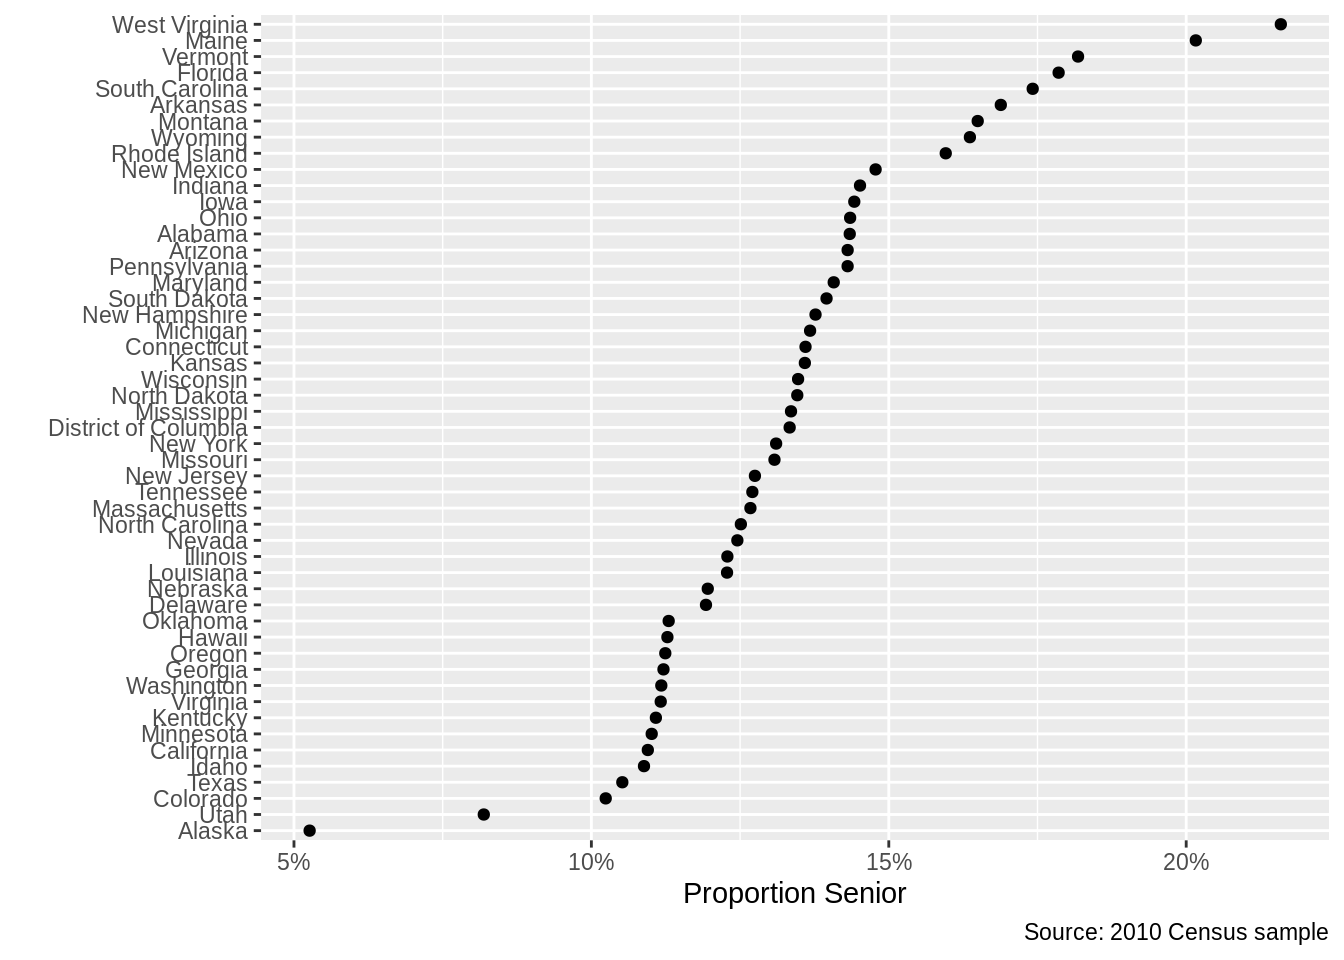
\includegraphics{prefresher_files/figure-latex/unnamed-chunk-326-1.pdf}

\hypertarget{swing-justice}{%
\subsection*{2 Swing Justice}\label{swing-justice}}
\addcontentsline{toc}{subsection}{2 Swing Justice}

\begin{Shaded}
\begin{Highlighting}[]
\NormalTok{justices <-}\StringTok{ }\KeywordTok{read_csv}\NormalTok{(}\StringTok{"input/justices_court-median.csv"}\NormalTok{)}
\end{Highlighting}
\end{Shaded}

Keep justices who are in the dataset in 2016,

\begin{Shaded}
\begin{Highlighting}[]
\NormalTok{in_}\DecValTok{2017}\NormalTok{ <-}\StringTok{ }\NormalTok{justices }\OperatorTok
\StringTok{  }\KeywordTok{filter}\NormalTok{(term }\OperatorTok{==}\StringTok{ }\DecValTok{2016}\NormalTok{) }\OperatorTok
\StringTok{  }\KeywordTok{distinct}\NormalTok{(justice) }\OperatorTok\StringTok{ }\CommentTok{# unique values}
\StringTok{  }\KeywordTok{mutate}\NormalTok{(}\DataTypeTok{present_2016 =} \DecValTok{1}\NormalTok{) }\CommentTok{# keep an indicator to distinguish from rest after merge}

\NormalTok{df_indicator <-}\StringTok{ }\NormalTok{justices }\OperatorTok
\StringTok{  }\KeywordTok{left_join}\NormalTok{(in_}\DecValTok{2017}\NormalTok{)}
\end{Highlighting}
\end{Shaded}

\begin{verbatim}
## Joining, by = "justice"
\end{verbatim}

All together

\begin{Shaded}
\begin{Highlighting}[]
\KeywordTok{ggplot}\NormalTok{(df_indicator, }\KeywordTok{aes}\NormalTok{(}\DataTypeTok{x =}\NormalTok{ term, }\DataTypeTok{y =}\NormalTok{ idealpt, }\DataTypeTok{group =}\NormalTok{ justice_id)) }\OperatorTok{+}
\StringTok{  }\KeywordTok{geom_line}\NormalTok{(}\KeywordTok{aes}\NormalTok{(}\DataTypeTok{y =}\NormalTok{ median_idealpt), }\DataTypeTok{color =} \StringTok{"red"}\NormalTok{, }\DataTypeTok{size =} \DecValTok{2}\NormalTok{, }\DataTypeTok{alpha =} \FloatTok{0.1}\NormalTok{) }\OperatorTok{+}
\StringTok{  }\KeywordTok{geom_line}\NormalTok{(}\DataTypeTok{alpha =} \FloatTok{0.5}\NormalTok{) }\OperatorTok{+}
\StringTok{  }\KeywordTok{geom_line}\NormalTok{(}\DataTypeTok{data =} \KeywordTok{filter}\NormalTok{(df_indicator, }\OperatorTok{!}\KeywordTok{is.na}\NormalTok{(present_}\DecValTok{2016}\NormalTok{))) }\OperatorTok{+}
\StringTok{  }\KeywordTok{geom_point}\NormalTok{(}\DataTypeTok{data =} \KeywordTok{filter}\NormalTok{(df_indicator, }\OperatorTok{!}\KeywordTok{is.na}\NormalTok{(present_}\DecValTok{2016}\NormalTok{), term }\OperatorTok{==}\StringTok{ }\DecValTok{2016}\NormalTok{)) }\OperatorTok{+}
\StringTok{  }\KeywordTok{geom_text_repel}\NormalTok{(}
    \DataTypeTok{data =} \KeywordTok{filter}\NormalTok{(df_indicator, term }\OperatorTok{==}\StringTok{ }\DecValTok{2016}\NormalTok{), }\KeywordTok{aes}\NormalTok{(}\DataTypeTok{label =}\NormalTok{ justice),}
    \DataTypeTok{nudge_x =} \DecValTok{10}\NormalTok{,}
    \DataTypeTok{direction =} \StringTok{"y"}
\NormalTok{  ) }\OperatorTok{+}\StringTok{ }\CommentTok{# labels nudged and vertical}
\StringTok{  }\KeywordTok{scale_x_continuous}\NormalTok{(}\DataTypeTok{breaks =} \KeywordTok{seq}\NormalTok{(}\DecValTok{1940}\NormalTok{, }\DecValTok{2020}\NormalTok{, }\DecValTok{10}\NormalTok{), }\DataTypeTok{limits =} \KeywordTok{c}\NormalTok{(}\DecValTok{1937}\NormalTok{, }\DecValTok{2020}\NormalTok{)) }\OperatorTok{+}\StringTok{ }\CommentTok{# axis breaks}
\StringTok{  }\KeywordTok{scale_y_continuous}\NormalTok{(}\DataTypeTok{limits =} \KeywordTok{c}\NormalTok{(}\OperatorTok{-}\DecValTok{5}\NormalTok{, }\DecValTok{5}\NormalTok{)) }\OperatorTok{+}\StringTok{ }\CommentTok{# axis limits}
\StringTok{  }\KeywordTok{labs}\NormalTok{(}
    \DataTypeTok{x =} \StringTok{"SCOTUS Term"}\NormalTok{,}
    \DataTypeTok{y =} \StringTok{"Estimated Martin-Quinn Ideal Point"}\NormalTok{,}
    \DataTypeTok{caption =} \StringTok{"Outliers capped at -5 to 5. Red lines indicate median justice. Current justices of the 2017 Court in black."}
\NormalTok{  ) }\OperatorTok{+}
\StringTok{  }\KeywordTok{theme_bw}\NormalTok{()}
\end{Highlighting}
\end{Shaded}

\begin{verbatim}
## Warning: Removed 30 rows containing missing values (geom_path).
\end{verbatim}

\begin{verbatim}
## Warning: Removed 19 rows containing missing values (geom_path).
\end{verbatim}

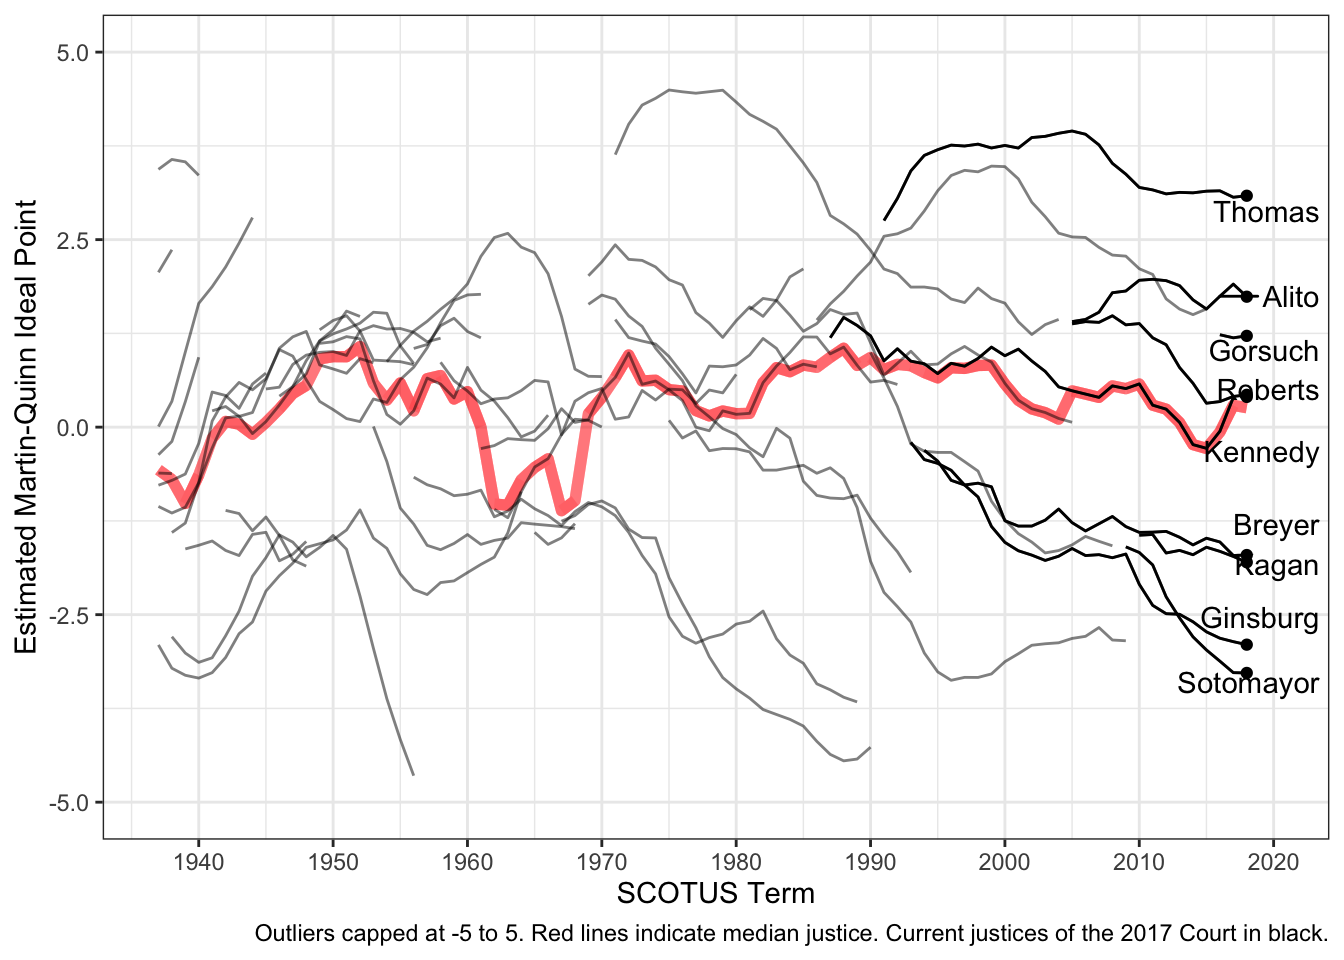
\includegraphics{prefresher_files/figure-latex/unnamed-chunk-329-1.pdf}

\hypertarget{chapter-refrobjloops-objects-and-loops}{%
\section{Chapter \ref{robjloops}: Objects and Loops}\label{chapter-refrobjloops-objects-and-loops}}

\begin{Shaded}
\begin{Highlighting}[]
\NormalTok{cen10 <-}\StringTok{ }\KeywordTok{read_csv}\NormalTok{(}\StringTok{"input/usc2010_001percent.csv"}\NormalTok{)}
\NormalTok{sample_acs <-}\StringTok{ }\KeywordTok{read_csv}\NormalTok{(}\StringTok{"input/acs2015_1percent.csv"}\NormalTok{)}
\end{Highlighting}
\end{Shaded}

\hypertarget{checkpoint-3}{%
\subsection*{Checkpoint \#3}\label{checkpoint-3}}
\addcontentsline{toc}{subsection}{Checkpoint \#3}

\begin{Shaded}
\begin{Highlighting}[]
\NormalTok{cen10 }\OperatorTok
\StringTok{  }\KeywordTok{group_by}\NormalTok{(city) }\OperatorTok
\StringTok{  }\KeywordTok{summarise}\NormalTok{(}\DataTypeTok{avg_age =} \KeywordTok{mean}\NormalTok{(age)) }\OperatorTok
\StringTok{  }\KeywordTok{arrange}\NormalTok{(}\KeywordTok{desc}\NormalTok{(avg_age)) }\OperatorTok
\StringTok{  }\KeywordTok{slice}\NormalTok{(}\DecValTok{1}\OperatorTok{:}\DecValTok{10}\NormalTok{)}
\end{Highlighting}
\end{Shaded}

\begin{verbatim}
## # A tibble: 10 x 2
##    city                 avg_age
##    <chr>                  <dbl>
##  1 Sterling Heights, MI    53.2
##  2 Waterbury, CT           49.3
##  3 Antioch, CA             49  
##  4 Little Rock, AR         46.9
##  5 Roseville, CA           43.3
##  6 Port St. Lucie, FL      42.8
##  7 Huntington Beach, CA    42.3
##  8 Pittsburgh, PA          42.2
##  9 Cambridge, MA           41.8
## 10 Alexandria, VA          41.8
\end{verbatim}

\hypertarget{exercise-1}{%
\subsection*{Exercise 1}\label{exercise-1}}
\addcontentsline{toc}{subsection}{Exercise 1}

\begin{Shaded}
\begin{Highlighting}[]
\KeywordTok{colnames}\NormalTok{(sample_acs)}
\end{Highlighting}
\end{Shaded}

\begin{verbatim}
##  [1] "serial"            "pernum"            "hhwt"             
##  [4] "perwt"             "state"             "county_identified"
##  [7] "puma"              "city"              "sex"              
## [10] "age"               "birthyr"           "race"             
## [13] "hispan"            "educ"              "citizen"          
## [16] "yrnatur"
\end{verbatim}

\begin{Shaded}
\begin{Highlighting}[]
\KeywordTok{unique}\NormalTok{(sample_acs}\OperatorTok{$}\NormalTok{citizen)}
\end{Highlighting}
\end{Shaded}

\begin{verbatim}
## [1] "Born in the US"                                                           
## [2] "US citizen by naturalization"                                             
## [3] "Not a citizen of the US"                                                  
## [4] "Born abroad of American parent(s)"                                        
## [5] "Born in Puerto Rico, Guam, the US Virgin Islands,or the Northern Marianas"
\end{verbatim}

\begin{Shaded}
\begin{Highlighting}[]
\KeywordTok{mean}\NormalTok{(sample_acs}\OperatorTok{$}\NormalTok{citizen }\OperatorTok{!=}\StringTok{ "Not a citizen of the US"}\NormalTok{)}
\end{Highlighting}
\end{Shaded}

\begin{verbatim}
## [1] 0.9419765
\end{verbatim}

\hypertarget{exercise-3}{%
\subsection*{Exercise 3}\label{exercise-3}}
\addcontentsline{toc}{subsection}{Exercise 3}

\begin{Shaded}
\begin{Highlighting}[]
\NormalTok{states_of_interest <-}\StringTok{ }\KeywordTok{c}\NormalTok{(}\StringTok{"California"}\NormalTok{, }\StringTok{"Massachusetts"}\NormalTok{, }\StringTok{"New Hampshire"}\NormalTok{, }\StringTok{"Washington"}\NormalTok{)}

\ControlFlowTok{for}\NormalTok{ (state_i }\ControlFlowTok{in}\NormalTok{ states_of_interest) \{}
\NormalTok{  state_subset <-}\StringTok{ }\NormalTok{cen10 }\OperatorTok\StringTok{ }\KeywordTok{filter}\NormalTok{(state }\OperatorTok{==}\StringTok{ }\NormalTok{state_i)}

  \KeywordTok{print}\NormalTok{(state_i)}

  \KeywordTok{print}\NormalTok{(}\KeywordTok{table}\NormalTok{(state_subset}\OperatorTok{$}\NormalTok{race, state_subset}\OperatorTok{$}\NormalTok{sex))}
\NormalTok{\}}
\end{Highlighting}
\end{Shaded}

\begin{verbatim}
## [1] "California"
##                                   
##                                    Female Male
##   American Indian or Alaska Native     21   21
##   Black/Negro                         127  126
##   Chinese                              76   65
##   Japanese                             15   12
##   Other Asian or Pacific Islander     182  177
##   Other race, nec                     283  302
##   Three or more major races             7    7
##   Two major races                      91   83
##   White                              1085 1083
## [1] "Massachusetts"
##                                   
##                                    Female Male
##   American Indian or Alaska Native      4    1
##   Black/Negro                          21   17
##   Chinese                               8    7
##   Japanese                              1    1
##   Other Asian or Pacific Islander      14   14
##   Other race, nec                       9   17
##   Two major races                      10    8
##   White                               272  243
## [1] "New Hampshire"
##                                   
##                                    Female Male
##   American Indian or Alaska Native      1    0
##   Black/Negro                           0    1
##   Chinese                               0    1
##   Japanese                              1    0
##   Other Asian or Pacific Islander       2    1
##   Other race, nec                       1    0
##   Two major races                       0    1
##   White                                66   63
## [1] "Washington"
##                                   
##                                    Female Male
##   American Indian or Alaska Native      9    5
##   Black/Negro                          11    9
##   Chinese                               2    7
##   Japanese                              4    0
##   Other Asian or Pacific Islander      28   18
##   Other race, nec                      19   18
##   Three or more major races             0    2
##   Two major races                      17   16
##   White                               267  257
\end{verbatim}

\hypertarget{exercise-4}{%
\subsection*{Exercise 4}\label{exercise-4}}
\addcontentsline{toc}{subsection}{Exercise 4}

\begin{Shaded}
\begin{Highlighting}[]
\NormalTok{race_d <-}\StringTok{ }\KeywordTok{c}\NormalTok{()}
\NormalTok{state_d <-}\StringTok{ }\KeywordTok{c}\NormalTok{()}
\NormalTok{proportion_d <-}\StringTok{ }\KeywordTok{c}\NormalTok{()}
\NormalTok{answer <-}\StringTok{ }\KeywordTok{data.frame}\NormalTok{(race_d, state_d, proportion_d)}
\end{Highlighting}
\end{Shaded}

Then

\begin{Shaded}
\begin{Highlighting}[]
\ControlFlowTok{for}\NormalTok{ (state }\ControlFlowTok{in}\NormalTok{ states_of_interest) \{}
  \ControlFlowTok{for}\NormalTok{ (race }\ControlFlowTok{in} \KeywordTok{unique}\NormalTok{(cen10}\OperatorTok{$}\NormalTok{race)) \{}
\NormalTok{    race_state_num <-}\StringTok{ }\KeywordTok{nrow}\NormalTok{(cen10[cen10}\OperatorTok{$}\NormalTok{race }\OperatorTok{==}\StringTok{ }\NormalTok{race }\OperatorTok{&}\StringTok{ }\NormalTok{cen10}\OperatorTok{$}\NormalTok{state }\OperatorTok{==}\StringTok{ }\NormalTok{state, ])}
\NormalTok{    state_pop <-}\StringTok{ }\KeywordTok{nrow}\NormalTok{(cen10[cen10}\OperatorTok{$}\NormalTok{state }\OperatorTok{==}\StringTok{ }\NormalTok{state, ])}
\NormalTok{    race_perc <-}\StringTok{ }\KeywordTok{round}\NormalTok{(}\DecValTok{100} \OperatorTok{*}\StringTok{ }\NormalTok{(race_state_num }\OperatorTok{/}\StringTok{ }\NormalTok{(state_pop)), }\DataTypeTok{digits =} \DecValTok{2}\NormalTok{)}
\NormalTok{    line <-}\StringTok{ }\KeywordTok{data.frame}\NormalTok{(}\DataTypeTok{race_d =}\NormalTok{ race, }\DataTypeTok{state_d =}\NormalTok{ state, }\DataTypeTok{proportion_d =}\NormalTok{ race_perc)}
\NormalTok{    answer <-}\StringTok{ }\KeywordTok{rbind}\NormalTok{(answer, line)}
\NormalTok{  \}}
\NormalTok{\}}
\end{Highlighting}
\end{Shaded}

\hypertarget{chapter-refdempeace-demoratic-peace-project}{%
\section{Chapter \ref{dempeace}: Demoratic Peace Project}\label{chapter-refdempeace-demoratic-peace-project}}

\hypertarget{task-1-data-input-and-standardization-1}{%
\subsection*{Task 1: Data Input and Standardization}\label{task-1-data-input-and-standardization-1}}
\addcontentsline{toc}{subsection}{Task 1: Data Input and Standardization}

\begin{Shaded}
\begin{Highlighting}[]
\NormalTok{mid_b <-}\StringTok{ }\KeywordTok{read_csv}\NormalTok{(}\StringTok{"input/MIDB_4.2.csv"}\NormalTok{)}
\NormalTok{polity <-}\StringTok{ }\KeywordTok{read_excel}\NormalTok{(}\StringTok{"input/p4v2017.xls"}\NormalTok{)}
\end{Highlighting}
\end{Shaded}

\hypertarget{task-2-data-merging-1}{%
\subsection*{Task 2: Data Merging}\label{task-2-data-merging-1}}
\addcontentsline{toc}{subsection}{Task 2: Data Merging}

\begin{Shaded}
\begin{Highlighting}[]
\NormalTok{mid_y_by_y <-}\StringTok{ }\KeywordTok{data_frame}\NormalTok{(}\DataTypeTok{ccode =} \KeywordTok{numeric}\NormalTok{(),}
                               \DataTypeTok{year =} \KeywordTok{numeric}\NormalTok{(),}
                               \DataTypeTok{dispute =} \KeywordTok{numeric}\NormalTok{())}
\KeywordTok{colnames}\NormalTok{(mid_b)}
\ControlFlowTok{for}\NormalTok{(i }\ControlFlowTok{in} \DecValTok{1}\OperatorTok{:}\KeywordTok{nrow}\NormalTok{(mid_b)) \{}
\NormalTok{    x <-}\StringTok{ }\KeywordTok{data_frame}\NormalTok{(}\DataTypeTok{ccode =}\NormalTok{ mid_b}\OperatorTok{$}\NormalTok{ccode[i], }\CommentTok{## row i's country}
    \DataTypeTok{year =}\NormalTok{ mid_b}\OperatorTok{$}\NormalTok{styear[i]}\OperatorTok{:}\NormalTok{mid_b}\OperatorTok{$}\NormalTok{endyear[i],  }\CommentTok{## sequence of years for dispute in row i}
    \DataTypeTok{dispute =} \DecValTok{1}\NormalTok{)}\CommentTok{## there was a dispute}
\NormalTok{    mid_y_by_y <-}\StringTok{ }\KeywordTok{rbind}\NormalTok{(mid_y_by_y, x)}
\NormalTok{\}}

\NormalTok{merged_mid_polity <-}\StringTok{ }\KeywordTok{left_join}\NormalTok{(polity,}
                 \KeywordTok{distinct}\NormalTok{(mid_y_by_y),}
                 \DataTypeTok{by =} \KeywordTok{c}\NormalTok{(}\StringTok{"ccode"}\NormalTok{, }\StringTok{"year"}\NormalTok{))}
\end{Highlighting}
\end{Shaded}

\hypertarget{task-3-tabulations-and-visualization-1}{%
\subsection*{Task 3: Tabulations and Visualization}\label{task-3-tabulations-and-visualization-1}}
\addcontentsline{toc}{subsection}{Task 3: Tabulations and Visualization}

\begin{Shaded}
\begin{Highlighting}[]
\CommentTok{#don't include the -88, -77, -66 values in calculating the mean of polity}
\NormalTok{mean_polity_by_year <-}\StringTok{ }\NormalTok{merged_mid_polity }\OperatorTok\StringTok{ }\KeywordTok{group_by}\NormalTok{(year) }\OperatorTok\StringTok{ }\KeywordTok{summarise}\NormalTok{(}\DataTypeTok{mean_polity =} \KeywordTok{mean}\NormalTok{(polity[}\KeywordTok{which}\NormalTok{(polity }\OperatorTok{<}\DecValTok{11} \OperatorTok{&}\StringTok{ }\NormalTok{polity }\OperatorTok{>}\StringTok{ }\DecValTok{-11}\NormalTok{)]))}

\NormalTok{mean_polity_by_year_ordered <-}\StringTok{ }\KeywordTok{arrange}\NormalTok{(mean_polity_by_year, year) }

\NormalTok{mean_polity_by_year_mid <-}\StringTok{ }\NormalTok{merged_mid_polity }\OperatorTok\StringTok{ }\KeywordTok{group_by}\NormalTok{(year, dispute) }\OperatorTok\StringTok{ }\KeywordTok{summarise}\NormalTok{(}\DataTypeTok{mean_polity_mid =} \KeywordTok{mean}\NormalTok{(polity[}\KeywordTok{which}\NormalTok{(polity }\OperatorTok{<}\DecValTok{11} \OperatorTok{&}\StringTok{ }\NormalTok{polity }\OperatorTok{>}\StringTok{ }\DecValTok{-11}\NormalTok{)]))}

\NormalTok{mean_polity_by_year_mid_ordered <-}\StringTok{ }\KeywordTok{arrange}\NormalTok{(mean_polity_by_year_mid, year) }

\NormalTok{mean_polity_no_mid <-}\StringTok{ }\NormalTok{mean_polity_by_year_mid_ordered }\OperatorTok\StringTok{ }\KeywordTok{filter}\NormalTok{(dispute }\OperatorTok{==}\StringTok{ }\DecValTok{0}\NormalTok{)}
\NormalTok{mean_polity_yes_mid <-}\StringTok{ }\NormalTok{mean_polity_by_year_mid_ordered }\OperatorTok\StringTok{ }\KeywordTok{filter}\NormalTok{(dispute }\OperatorTok{==}\StringTok{ }\DecValTok{1}\NormalTok{)}


\NormalTok{answer <-}\StringTok{ }\KeywordTok{ggplot}\NormalTok{(}\DataTypeTok{data =}\NormalTok{ mean_polity_by_year_ordered, }\KeywordTok{aes}\NormalTok{(}\DataTypeTok{x =}\NormalTok{ year, }\DataTypeTok{y =}\NormalTok{ mean_polity)) }\OperatorTok{+}
\StringTok{  }\KeywordTok{geom_line}\NormalTok{() }\OperatorTok{+}
\StringTok{  }\KeywordTok{labs}\NormalTok{(}\DataTypeTok{y =} \StringTok{"Mean Polity Score"}\NormalTok{,}
       \DataTypeTok{x =} \StringTok{""}\NormalTok{) }\OperatorTok{+}
\StringTok{  }\KeywordTok{geom_vline}\NormalTok{(}\DataTypeTok{xintercept =} \KeywordTok{c}\NormalTok{(}\DecValTok{1914}\NormalTok{, }\DecValTok{1929}\NormalTok{, }\DecValTok{1939}\NormalTok{, }\DecValTok{1989}\NormalTok{, }\DecValTok{2008}\NormalTok{), }\DataTypeTok{linetype =} \StringTok{"dashed"}\NormalTok{)}

\NormalTok{answer }\OperatorTok{+}\StringTok{ }\KeywordTok{geom_line}\NormalTok{(}\DataTypeTok{data =}\NormalTok{mean_polity_no_mid, }\KeywordTok{aes}\NormalTok{(}\DataTypeTok{x =}\NormalTok{ year, }\DataTypeTok{y =}\NormalTok{ mean_polity_mid), }\DataTypeTok{col =} \StringTok{"indianred"}\NormalTok{) }\OperatorTok{+}\StringTok{ }\KeywordTok{geom_line}\NormalTok{(}\DataTypeTok{data =}\NormalTok{mean_polity_yes_mid, }\KeywordTok{aes}\NormalTok{(}\DataTypeTok{x =}\NormalTok{ year, }\DataTypeTok{y =}\NormalTok{ mean_polity_mid), }\DataTypeTok{col =} \StringTok{"dodgerblue"}\NormalTok{)}
\end{Highlighting}
\end{Shaded}

\hypertarget{chapter-refsimulation-simulation}{%
\section{Chapter \ref{simulation}: Simulation}\label{chapter-refsimulation-simulation}}

\hypertarget{census-sampling-1}{%
\subsection{Census Sampling}\label{census-sampling-1}}

\begin{Shaded}
\begin{Highlighting}[]
\NormalTok{pop <-}\StringTok{ }\KeywordTok{read_csv}\NormalTok{(}\StringTok{"input/usc2010_001percent.csv"}\NormalTok{)}
\end{Highlighting}
\end{Shaded}

\begin{verbatim}
## Parsed with column specification:
## cols(
##   year = col_double(),
##   serial = col_double(),
##   pernum = col_double(),
##   region = col_character(),
##   state = col_character(),
##   countyfips = col_double(),
##   city = col_character(),
##   cpuma0010 = col_double(),
##   sex = col_character(),
##   age = col_double(),
##   race = col_character(),
##   hhtype = col_character(),
##   relate = col_character()
## )
\end{verbatim}

\begin{Shaded}
\begin{Highlighting}[]
\KeywordTok{mean}\NormalTok{(pop}\OperatorTok{$}\NormalTok{race }\OperatorTok{!=}\StringTok{ "White"}\NormalTok{)}
\end{Highlighting}
\end{Shaded}

\begin{verbatim}
## [1] 0.2806517
\end{verbatim}

\begin{Shaded}
\begin{Highlighting}[]
\KeywordTok{set.seed}\NormalTok{(}\DecValTok{1669482}\NormalTok{)}
\NormalTok{samp <-}\StringTok{ }\KeywordTok{sample_n}\NormalTok{(pop, }\DecValTok{100}\NormalTok{)}
\KeywordTok{mean}\NormalTok{(samp}\OperatorTok{$}\NormalTok{race }\OperatorTok{!=}\StringTok{ "White"}\NormalTok{)}
\end{Highlighting}
\end{Shaded}

\begin{verbatim}
## [1] 0.31
\end{verbatim}

\begin{Shaded}
\begin{Highlighting}[]
\NormalTok{ests <-}\StringTok{ }\KeywordTok{c}\NormalTok{()}
\KeywordTok{set.seed}\NormalTok{(}\DecValTok{1669482}\NormalTok{)}

\ControlFlowTok{for}\NormalTok{ (i }\ControlFlowTok{in} \DecValTok{1}\OperatorTok{:}\DecValTok{20}\NormalTok{) \{}
\NormalTok{  samp <-}\StringTok{ }\KeywordTok{sample_n}\NormalTok{(pop, }\DecValTok{100}\NormalTok{)}
\NormalTok{  ests[i] <-}\StringTok{ }\KeywordTok{mean}\NormalTok{(samp}\OperatorTok{$}\NormalTok{race }\OperatorTok{!=}\StringTok{ "White"}\NormalTok{)}
\NormalTok{\}}


\KeywordTok{mean}\NormalTok{(ests)}
\end{Highlighting}
\end{Shaded}

\begin{Shaded}
\begin{Highlighting}[]
\NormalTok{pop_with_prop <-}\StringTok{ }\KeywordTok{mutate}\NormalTok{(pop, }\DataTypeTok{propensity =} \KeywordTok{ifelse}\NormalTok{(race }\OperatorTok{!=}\StringTok{ "White"}\NormalTok{, }\FloatTok{0.9}\NormalTok{, }\DecValTok{1}\NormalTok{))}
\end{Highlighting}
\end{Shaded}

\begin{Shaded}
\begin{Highlighting}[]
\NormalTok{ests <-}\StringTok{ }\KeywordTok{c}\NormalTok{()}
\KeywordTok{set.seed}\NormalTok{(}\DecValTok{1669482}\NormalTok{)}

\ControlFlowTok{for}\NormalTok{ (i }\ControlFlowTok{in} \DecValTok{1}\OperatorTok{:}\DecValTok{20}\NormalTok{) \{}
\NormalTok{  samp <-}\StringTok{ }\KeywordTok{sample_n}\NormalTok{(pop_with_prop, }\DecValTok{100}\NormalTok{, }\DataTypeTok{weight =}\NormalTok{ propensity)}
\NormalTok{  ests[i] <-}\StringTok{ }\KeywordTok{mean}\NormalTok{(samp}\OperatorTok{$}\NormalTok{race }\OperatorTok{!=}\StringTok{ "White"}\NormalTok{)}
\NormalTok{\}}

\KeywordTok{mean}\NormalTok{(ests)}
\end{Highlighting}
\end{Shaded}

\begin{Shaded}
\begin{Highlighting}[]
\NormalTok{ests <-}\StringTok{ }\KeywordTok{c}\NormalTok{()}
\KeywordTok{set.seed}\NormalTok{(}\DecValTok{1669482}\NormalTok{)}

\ControlFlowTok{for}\NormalTok{ (i }\ControlFlowTok{in} \DecValTok{1}\OperatorTok{:}\DecValTok{20}\NormalTok{) \{}
\NormalTok{  samp <-}\StringTok{ }\KeywordTok{sample_n}\NormalTok{(pop_with_prop, }\DecValTok{10000}\NormalTok{, }\DataTypeTok{weight =}\NormalTok{ propensity)}
\NormalTok{  ests[i] <-}\StringTok{ }\KeywordTok{mean}\NormalTok{(samp}\OperatorTok{$}\NormalTok{race }\OperatorTok{!=}\StringTok{ "White"}\NormalTok{)}
\NormalTok{\}}

\KeywordTok{mean}\NormalTok{(ests)}
\end{Highlighting}
\end{Shaded}


\end{document}
